\documentclass[ignorenonframetext,notheorems,aspectratio=1610]{beamer}
\usetheme[compress]{Madrid}
\usecolortheme{iwr}
\usepackage{tikz,tikzscale}
\usetikzlibrary{snakes}
\usepackage{mathsim}
\usepackage{xr}
\externaldocument{awa}
\externaldocument{explicit}
\externaldocument{implicit}
\externaldocument{lmm}
\externaldocument{rwa}
\externaldocument{newton}
\externaldocument{fd}
\externaldocument{appendix}
\usepackage{mfirstuc}
\usepackage{mathtools}  
\mathtoolsset{showonlyrefs}

\makeatletter
\def\TH@with[#1]#2#3{\begin{block}{\capitalisewords{#2} \ref{#2:#3} (#1)}}
\def\TH@without#1#2{\begin{block}{\capitalisewords{#1} \ref{#1:#2}}}
\def\TH{\@ifnextchar[{\TH@with}{\TH@without}}%
\def\endTH{\end{block}}
\makeatother
\def\footnote#1{}

% Definitions for Runge-Kutta-Koefficients
\def\rks{s}  % Number of steps
\def\rka{a}  % Coefficient matrix
\def\rkb{b}  % Quadrature weights
\def\rkc{c}  % Quadrature points
\def\rkg{g}  % Intermediate points

\def\lmms{s}

% Definitions for boundary value problems
\def\rwaa{B_a}
\def\rwab{B_b}

\title{\textbf{Numerical Analysis \\of\\
    Ordinary Differential Equations}}
\author{Guido Kanschat}
\date{\today}
\begin{document}
\frame{\maketitle}
\frame{\frametitle{Overview}\tableofcontents[hideallsubsections]}
\section{Initial Value Problems and their Properties}
\frame{\tableofcontents[currentsection,hideothersubsections]}
\subsection{Modeling with ordinary differential equations}
\subsection{Introduction to initial value problems}

\frame{\begin{Definition}{explicit-ode}{Explicit differential equation}
  \defindex{ordinary differential equation!explicit} An \define{explicit
    differential equation} of first order is a equation of the form
  \begin{align}
    \label{eq:awa:ode}
    u'(t) &= f(t,u(t))\\
    \text{or shorter:}\qquad u'&=f(t,u). \notag
  \end{align}
  A differential equation of order $n$ is called explicit, if it is of
  the form
  \begin{gather*}
    u^{(n)}(t) = F\left(t, u(t), u'(t), \ldots, u^{(n-1)}(t)\right)
  \end{gather*}
\end{Definition}}
\frame{\begin{Lemma}{first-order}
  Every differential equation of higher order can be written as a
  system of first-order differential equations. If the equation is
  explicit, then the system is explicit.
\end{Lemma}}
\frame{\begin{Definition}{local-solution}
    \label{def:awa:local solution}
  \defindex{solution!local} We call a continuously differentiable
  function $u(t)$ with $u(t_0) = 0$ a \define{local solution} of the
  IVP~\eqref{eq:awa}, if there exists a neighborhood $J$ of the point
  in time $t_0$ in which $u$ and $f(t,u(t))$ are defined and if the
  equation~\eqref{eq:awa:2} holds for all $t\in J$.
\end{Definition}}
\frame{\begin{Lemma}{volterra}
  Under the assumption that the right hand side $f$ is continuous in
  both arguments, the function $u(t)$ is a solution of the initial
  value problem~\eqref{eq:awa} if and only if it is a solution of the
  \define{Volterra integral equation} (VIE) \index{VIE!see{Volterra
      integral equation}}
  \begin{gather}
    \label{eq:volterra}
    u(t) = u_0 + \int_{t_0}^t f\bigl(s,u(s)\bigr)\ds.
  \end{gather}
  The formulation as integral equation allows on the other hand a more
  general solution term, because the problem is already well-posed for
  functions $f(t,u)$, which are just integrable with respect to $t$.
  In that case the solution $u$ would be just absolutely continuous
  and not continuously differentiable.
\end{Lemma}

%%% Local Variables: 
%%% mode: latex
%%% TeX-master: "../notes"
%%% End: 
}
\frame{\begin{Theorem*}{peano}{Peano's existence theorem}
  \defindex{Peano's theorem}
  \label{satz:peano}
  Let the function $f(t,u)$ be continuous on the closed set
  \begin{gather*}
    \overline D =\bigl\{
    (t,u) \in \R\times\R^d \;\big|
    \;|t-t_0| \le \alpha,\;
    |u-u_0|\le\beta
    \bigr\},
  \end{gather*}
  where $\alpha,\beta>0$. Then there exists a solution
    $u(t) \in C^1(I)$
  on the interval
    $I=[t_0-T,t_0+T]$
  with
  \begin{gather*}
    T=\min\left(\alpha ,\frac{\beta}{M}\right),\;
    M=\max_{(t,u)\in \overline D} \ |f(t,u)|.
  \end{gather*}
\end{Theorem*}
}
\frame{\begin{Theorem*}{peano-continuation}{Peano's continuation theorem}
  Let the assumptions of Theorem~\ref{satz:peano} hold. Then, the
  solution can be extended to an interval $I_m = [t_-, t_+]$ such that
  the points $\bigl(t_-,u(t_-)\bigr)$ and $\bigl(t_+,u(t_+)\bigr)$ are
  on the boundary of $\overline D$. Neither the values of $t$, nor of
  $u(t)$ need to be bounded as long as $f$ remains bounded.
\end{Theorem*}}

\subsection{Linear differential equations
  and Grönwall's inequality}

\frame{\begin{Definition}{linear-ode}
    \defindex{ordinary differential equation!linear} An IVP according to
  definition ~\ref{Definition:IVP} is called \textbf{linear} \defindex{linear
    differential equation} if the right hand side $f$ is an affine
  function of $u$. Thus, we can write it in the form
  \begin{subequations}    
    \label{eq:awa:4}
    \begin{xalignat}{2}
      \label{eq:awa:5}
      u'(t) &= A(t)u(t) + b(t)
      & \forall t &\in \R \\
      \label{eq:awa:6}
      u(t_0) &= u_0
    \end{xalignat}
  \end{subequations}
  with a continuous matrix function $A:\R\to \C^{d \times d}$. If in
  addition $b(t) \equiv 0$, we call it \define{homogeneous}.
\end{Definition}}
\frame{\begin{Definition}{integrating factor}
    Let be the matrix function $A:I\to \C^{d\times d}$ continuous.  Then
  the function defined by
  \begin{gather}
    \label{eq:awa:7}
    M(t) = \exp\left(-\int_{t_0}^t A(s) \ds\right)
  \end{gather}
  is called \define{integrating factor} of the
  equation~\eqref{eq:awa:5}.
\end{Definition}
\begin{Lemma}{linear-representation}
  % Voraussetzungen an A und b
  A solution of the IVP~\eqref{eq:awa:4} is given through the 
  representation
  \begin{gather}
    \label{eq:awa:8}
    u(t) =  M(t)^{-1}\left(u_0 + \int_{t_0}^t M(s) b(s) \ds\right)
  \end{gather}
  with the integrating factor $M(t)$ of the equation~\eqref{eq:awa:7}.
  This solution exists for all $t\in \R$.
\end{Lemma}


%%% Local Variables:
%%% mode: latex
%%% TeX-master: "../notes"
%%% End:
}
\frame{\begin{Lemma*}{gronwall}{Grönwall}
  Let be $w(t)$, $a(t)$ and $b(t)$ be nonnegative, integrable
  functions, such that $a(t)w(t)$ is integrable. Furthermore, let
  $b(t)$ be monotonically nondecreasing and let $w(t)$ satisfy the
  integral inequality
  \begin{gather}
    \label{eq:awa:10}
    w(t) \le b(t) + \int_{t_0}^t a(s)w(s)\ds,\qquad t\ge t_.
  \end{gather}
  Then, for almost all $t \ge t_0$ there holds:
  \begin{gather}
    \label{eq:awa:11}
    w(t) \le b(t) \exp\left( \int_{t_0}^t  a(s) \ds\right).
  \end{gather}
\end{Lemma*}

%%% Local Variables:
%%% mode: latex
%%% TeX-master: "../notes"
%%% End:
}

\subsection{Well-posedness of the IVP}

\frame{\begin{Definition}{hadamard} 
  A mathematical problem is called \define{well-posed} if the
  following \textbf{Hadamard conditions} are satisfied:
  \index{Hadamard conditions}
  \begin{enumerate}
  \item A solution exists.
  \item The solution is unique.
  \item The solution is continuously dependent on the data.
  \end{enumerate}
  The third condition in this form is purely qualitative. Typically,
  in order to characterize problems with good approximation
  properties, we will require \putindex{Lipschitz continuity}, which
  has a more quantitative character.
\end{Definition}

%%% Local Variables:
%%% mode: latex
%%% TeX-master: "../notes"
%%% End:
}
\frame{\begin{Theorem*}{awa-stability}{Stability}
  Let $f(t,u)$ and $g(t,u)$ be two continuous functions on a
  cylinder $D = I \times \Omega$ where the interval $I$ contains
  $t_0$ and $\Omega$ is a convex set in $\R^d$.  Furthermore, let
  $f$ admit a Lipschitz condition with constant $L$ on $D$. Let $u$
  and $v$ be solutions to the IVP
  \begin{xalignat}{2}
    \label{eq:awa:20}
    u'&=f(t,u) \quad\forall t\in I,& u(t_0)&= u_0,\\
    \label{eq:awa:21}
    v'&=g(t,v) \quad\forall t\in I,& v(t_0)&= v_0.
  \end{xalignat}
  Then, there holds
  \begin{gather}
    \label{eq:awa:22}
    \abs{u(t)-v(t)} \le e^{L|t-t_0|}
    \left[ \abs{u_0-v_0}
      + \int_{t_0}^{t} \max_{x\in\Omega}
      \abs{f(s,x)-g(s,x)}\ds
    \right].
  \end{gather}
\end{Theorem*}

%%% Local Variables:
%%% mode: latex
%%% TeX-master: "../notes"
%%% End:
}
\frame{\begin{Theorem*}{picardlindelof}{Picard-Lindelöf}
  \defindex{Picard-Lindelöf theorem} 
  Let $f(t,y)$ be continuous on a cylinder
  \begin{gather*}
    D = \{ (t,y) \in \R \times
    \R^d | \ |t-t_0| \le a, |y-u_0| \le b \}.
  \end{gather*}
  Let $f$ be bounded such that there is a constant $M = \max_D
  \abs{f}$ and satisfy the Lipschitz condition~\eqref{eq:awa:1} with
  constant $L$ on $D$.  Then the IVP
  \begin{gather*}
    \begin{split}
      u' &= f(t,u) \\ u(t_0) &= u_0
    \end{split}
  \end{gather*}
  is uniquely solvable on the interval
  $I = [t_0-T,t_0+T]$ where
  $T = \min \{ a, \frac{b}{M} \}$.
\end{Theorem*}

%%% Local Variables:
%%% mode: latex
%%% TeX-master: "../notes"
%%% End:
}

\section{Explicit One-Step Methods and Convergence}
\frame{\tableofcontents[currentsection,hideothersubsections]}
\subsection{Introduction}

\frame{\begin{Definition*}{one-step}{Explicit one-step method}
  \defindex{One-step method!explicit} An \textbf{explicit one-step
    method} \defindex{Explicit one-step method} is a method which,
  given $u_0$ at $t_0 = 0$ computes a sequence of approximations
  $y_1\,\dots,y_n$ to the solution of an IVP in the time steps
  $t_1,\dots,t_n$ using an update formula of the form\footnote{The adjective
  `explicit' is here in contrast to `implicit'
  one-step methods, where the increment function depends 
	on $y_{k}$ and equation~\eqref{eq:explicit:8} must be solved
        for $y_{k}$.}
  \begin{gather}
    \label{eq:explicit:8}
    y_{k} = y_{k-1} + h_{k} \verfahren_{h_k}(t_{k-1},y_{k-1}).
  \end{gather}
  The function $\verfahren()_{h_k}$ is called \define{increment
    function}.  We will often omit the index $h_k$ on
  $\verfahren_{h_k}()$ because it is clear that the method is always
  applied to time intervals.

  The method is called \textbf{one-step method}
  because the value $y_{k}$ explicitly depends only of the values
  $y_{k-1}$ and $f(t_{k-1}, y_{k-1})$, not on previous values.
\end{Definition*}

%%% Local Variables:
%%% mode: latex
%%% TeX-master: "../notes"
%%% End:
}
\frame{\begin{Example}{euler-linear-1}
  Given the IVP
  \begin{xalignat*}2
    u'  &= u,&
    u(0) &= 1,    
  \end{xalignat*}  
  the solution is $u(t) = e^t$. The Euler method reads
  \begin{gather*}
    y_1 = y_0 + h y_0.
  \end{gather*}
  The results for $h=1$ and $h=1/2$ are:
  \begin{center}
    \begin{tabular}{cc|ccc|ccc}
      \multicolumn{2}{c|}{exact}
      &\multicolumn{3}{c|}{$h=1$}
      &\multicolumn{3}{c}{$h=1/2$}\\\hline
      $t=0$ & 1           & $y_0$ & 1     && $y_0$ & 1 & \\
      $t=1$ & 2.71828     & $y_1$ & 2     & 0.718 & $y_2$ & 2.25  & 0.468\\
      $t=2$ & 7.38906     & $y_2$ & 4     & 3.389 & $y_4$ & 5.0625& 2.236\\\hline
      $t=k$ & $2.71828^k$ & $y_k$ & $2^k$ && $y_{2k}$ & $2.25^k$
    \end{tabular}    
  \end{center}
  We note that the error is growing in time. The approximation of the
  solution can be improved by shrinking $h$ from 1 to 1/2. The goal of
  error analysis will be establishing these dependencies.
\end{Example}

%%% Local Variables:
%%% mode: latex
%%% TeX-master: "../notes"
%%% End:
}

\subsection{Error analysis}
\begin{frame}
  \frametitle{Error decomposition}
  \centering
  \includegraphics[width=.49\textwidth]{fig/forward-error.tikz}
  \includegraphics[width=.49\textwidth]{fig/backward-error.tikz}
\end{frame}

\frame{\begin{Definition}{truncation-error}
  Let $u$ be a solution of the differential equation $u' = f(t,u)$
  on the interval $I_n = [t_{n-1}, t_{n}]$. Then, the \define{local
    error} of a discrete method $F$ is the difference between the
  solution $u_n$ of the differential equation at $t_n$ and the result
  of one time step~\eqref{eq:explicit:8} with this method with exact
  initial value:
  \begin{gather}
    \label{eq:explicit:6a}
    \eta_{n} = \eta_n(u) = u_{n} - \bigl[
    u_{n-1} + h_n \verfahren_{h_n}(t_{n-1}, u_{n-1})
    \bigr].
  \end{gather}
  The \define{truncation error} is the quotient of the local error and $h_n$:
  \begin{gather}
    \label{eq:explicit:6}
    \tau_{n} = \tau_n(u) = \frac{u_{n} - u_{n-1}}{h_n} - \verfahren_{h_n}(t_{n-1}, u_{n-1}).
  \end{gather}
  \defindex{order!of consistency}
  The one-step method $F_h(t,y)$ is \define{consistent} of \textbf{order} $p$ with
  the ODE, if there is a constant $c$ independent of $h$ such that for
  $h\to 0$:
  \begin{gather}
    \label{eq:explicit:3}
    \max\limits_n \abs{\tau_n} \le c h^p
  \end{gather}
\end{Definition}

%%% Local Variables:
%%% mode: latex
%%% TeX-master: "../notes"
%%% End:
}
\frame{\begin{Lemma*}{gronwall-discrete}{Discrete Grönwall inequality}
  \index{Grönwall's inequality} Let $(w_n)$, $(a_n)$ and $(b_n)$ be
  non-negative sequences of real numbers. Let $b_n$ be monotonically
  nondecreasing. Then, if
  \begin{gather}
    \label{eq:gronwall-discrete:1}
    w_0 \le b_0
    \quad\text{and}\quad
    \forall n\ge 1 :\;
    w_n \le \sum\limits_{k=0}^{n-1} a_k w_k + b_n,
  \end{gather}
  there holds
  \begin{gather}
    \label{eq:explicit:5}
    w_n \le \exp \left(\sum\limits_{k=1}^{n-1} a_k\right) b_n.
  \end{gather}
\end{Lemma*}

%%% Local Variables:
%%% mode: latex
%%% TeX-master: "../notes"
%%% End:
}
\frame{\begin{Theorem*}{stability-discrete}{Discrete stability}
  If $F(t,y)$ is Lipschitz continuous in $y$ for any $t=t_k$, $k<n$,
  with constant $L_h$, then the one-step method is \define{discretely
    stable}, i.~e. for arbitrary sequences $(y_n)$ and $(z_n)$, there
  holds: if $\eta_k(y)$ and $\eta_k(z)$ are both bounded independent
  of the sequences $(y_n)$ and $(z_n)$, then
  \begin{equation*}
    \abs{y_n - z_n}
    \le e^{L_h(t_n-t_0)} \left(
      \abs{y_0 - z_0}
      + \sum_{k=1}^n \abs{\eta_k(y) - \eta_k(z)}
    \right)
  \end{equation*}
\end{Theorem*}

%%% Local Variables:
%%% mode: latex
%%% TeX-master: "../notes"
%%% End:
}
\frame{\begin{Theorem*}{convergence-one-step}{Convergence of one-step methods}
  Let the one-step method $F(.,.)$ be consistent of order $p$ and
  discretely stable, that is, $F(.,.)$ is Lipschitz continuous in its
  second argument. Let $f(t,u)\in C^{p}$. Furthermore, let be
  $y_0 = u_0$. Then the method converges with order $p$ and there
  holds for $h = \max h_n$
  \begin{equation}
    \label{eq:convergence-onestep:1}
    \abs{u_n - y_n} \le c e^{L_h(t_n-t_0)} h^p,
  \end{equation}
  where the constant $c$ is independent of $h$.
\end{Theorem*}

%%% Local Variables:
%%% mode: latex
%%% TeX-master: "../notes"
%%% End:
}

\subsection{Runge-Kutta methods}

\frame{\begin{Definition}{erk}
  \defindex{Runge-Kutta method!explicit (ERK)}
  \index{ERK|see{Runge-Kutta method}} 
  An \textbf{explicit Runge-Kutta method (ERK)} is a
  one-step method with the representation
  \begin{subequations}
    \label{eq:explicit:1}
    \begin{xalignat}{2}
      \label{eq:explicit:1a}
      \rkg_i &= y_0 + h \sum_{j=1}^{i-1} \rka_{ij} k_j
      & i &= 1,\dots,\rks
      \\
      \label{eq:explicit:1b}
      k_i &= f\left(h \rkc_i, \rkg_i\right)
      & i &= 1,\dots,\rks
      \\
      \label{eq:explicit:1c}
      y_1 &= y_0 + h \sum_{i=1}^{\rks} \rkb_i k_i
    \end{xalignat}
  \end{subequations}
  In this method the values $h\rkc_i$ are the quadrature points
  on the interval $[0,h]$. The values $k_i$ are approximations to
  function values of the integrand in these points and the values $\rkg_i$ constitute
  approximations to the solution $u(h\rkc_i)$ in the quadrature
  points. This method uses $s$ intermediate values and is thus called
  an $\rks$-stage method.
\end{Definition}

%%% Local Variables:
%%% mode: latex
%%% TeX-master: "../notes"
%%% End:
}
\frame{\begin{Definition*}{butcher-tableau-erk}{Butcher tableau}
  It is customary to write Runge-Kutta methods in the form of a
  \define{Butcher tableau}, containing only the coefficients of
  equation~\eqref{eq:explicit:1} in the following matrix form:
\begin{gather}
  \label{eq:explicit:2}
  \begin{array}{c|ccccc}
    0 & \\
    \rkc_2 & \rka_{21} \\
    \rkc_3 & \rka_{31} & \rka_{32} \\
    \vdots & \vdots & \vdots & \ddots \\
    \rkc_\rks & \rka_{\rks1} & \rka_{\rks2} & \cdots & \rka_{\rks,\rks-1} \\
    \hline
    & \rkb_1 & \rkb_2 & \cdots & \rkb_{\rks-1} & \rkb_\rks \\
  \end{array}
\end{gather}
\end{Definition*}

%%% Local Variables:
%%% mode: latex
%%% TeX-master: "../notes"
%%% End:
}
\frame{\begin{Example*}{rk2}{Two-stage methods}
  \index{Euler method!modified} The \define{modified Euler method} is
  a variation of the Euler method of the following form:
  \begin{gather*}
    \begin{aligned}
      k_1 & = f(t_0,y_0) \\
      k_2 & = f(t_0 + \frac12 h, y_0 + h \frac12 k_1) \\
      y_{1} & = y_0 + h k_2
    \end{aligned}
    \qquad
    \begin{array}{c|cc}
      0 & \\
      \frac12 & \frac12 \\
      \hline
        & 0 & 1
    \end{array}
  \end{gather*}

  The so-called \define{Heun method} of order 2 is characterized
  through the equation
  \begin{gather*}
    \begin{aligned}
      k_1 & = f(t_0, y_0) \\
      k_2 & = f(t_0 + h, y_0 + h k_1) \\
      y_{1} & = y_0 + h ( \frac12 k_1 + \frac12 k_2 ) \\
    \end{aligned}
    \qquad
    \begin{array}{c|cc}
      0 & \\
      1 & 1 \\
      \hline
        & \frac12 & \frac12 \\
    \end{array}
  \end{gather*}
\end{Example*}

%%% Local Variables: 
%%% mode: latex
%%% TeX-master: "../notes"
%%% End: 
}
\frame{\begin{Example*}{rk4}{The classical Runge-Kutta method of 4th order}
  \defindex{Runge-Kutta method!four-stage}
  \begin{gather*}
    \begin{aligned}
      k_1 & = f(t_n, y_n) \\
      k_2 & = f(t_n + \frac12 h_n, y_n + \frac12 h_n k_1) \\
      k_3 & = f(t_n + \frac12 h_n, y_n + \frac12 h_n k_2) \\
      k_4 & = f(t_n + h_n, y_n + h_n k_3) \\
      y_{n+1} & = y_n + h_n ( \frac16 k_1 + \frac26 k_2 + \frac26 k_3 + \frac16 k_4 ) \\
    \end{aligned}
    \qquad
    \begin{array}{c|cccc}
      0 & \\
      \frac12 & \frac12 \\
      \frac12 & 0 & \frac12 \\
      1 & 0 & 0 & 1 \\
      \hline
        & \frac16 & \frac26 & \frac26 & \frac16 \\
    \end{array}
  \end{gather*}
  This formula is based on the Simpson rule as well, but it uses two
  approximations for the value in the center point. It is of fourth
  order.
\end{Example*}

%%% Local Variables:
%%% mode: latex
%%% TeX-master: "../notes"
%%% End:
}
\frame{\begin{Lemma}{rk-order-3-4}
  An autonomizable ERK with $s$ stages is consistent of third order, if
  and only if the following conditions are met:
  \begin{subequations}
    \label{eq:explicit:11}
    \begin{align}
      \label{eq:explicit:12}
      b_1 + \dots + b_s &= 1, \\
      \label{eq:explicit:13}
      b_1c_1 + \dots + b_s c_s &= 1/2, \\
      \label{eq:explicit:14}
      b_1c_1^2 + \dots + b_s c_s^2 &= 1/3, \\
      \label{eq:explicit:15}
      \sum\nolimits_{i,j} b_i a_{ij}c_j &= 1/6.
    \end{align}
    It is consistent of fourth order, if and only if additionally
    \begin{align}
    \label{eq:explicit:16}
    b_1c_1^3 + \dots + b_s c_s^3 &= 1/4, \\
    \label{eq:explicit:17}
    \sum\nolimits_{i,j} b_i c_i a_{ij} c_j &= 1/8, \\
    \label{eq:explicit:18}
    \sum\nolimits_{i,j} b_i a_{ij} c_j^2 &= 1/12, \\
    \label{eq:explicit:19}
    \sum\nolimits_{i,j,k} b_i a_{ij} a_{jk} c_k &= 1/24.
  \end{align}
  \end{subequations}
\end{Lemma}

%%% Local Variables:
%%% mode: latex
%%% TeX-master: "../notes"
%%% End:
}
\frame{\begin{Lemma}{taylor-u}
  The Taylor expansion of a single component of $u_1 = u(h)$ with
  respect to $h$ is
  \begin{gather}
    \label{eq:taylor-u:1}
    \begin{split}
      (u_1)_n &= (u_0)_n
      \\& + h f_n
      \\& + \frac{h^2}2 \sum_\lambda \partial_{\lambda} f_n f_\lambda
      \\& + \frac{h^3}6 \sum_{\lambda,\mu} \bigl[\partial_{\lambda\mu} f_n f_\lambda f_\mu
      + \partial_{\lambda}f_n \partial_{\mu}f_\lambda f_\mu\bigr]
      \\& + \frac{h^4}{24} \sum_{\lambda,\mu,\nu}
      \bigl[\partial_{\lambda\mu\nu} f_n f_\lambda f_\mu f_\nu
      + 3\partial_{\lambda\mu} f_n \partial_{m}f_\lambda f_\mu f_\nu
      % \\&+ \partial_{\lambda\mu} f_n \partial_{\nu}f_\mu f_\lambda f_\nu
      % \\&+ \partial_{\lambda\nu} f_n \partial_{\mu}f_\lambda f_\mu f_\nu
      \\&\hphantom{+\frac{h^4}{24} \sum_{\lambda,\mu,\nu}}
      + \partial_{\lambda}f_n \partial_{\mu\nu} f_\lambda f_\mu f_\nu
      + \partial_{\lambda}f_n \partial_{\mu} f_\lambda \partial_{\nu} f_\mu f_\nu
      \\&+\dots
    \end{split}
  \end{gather}
  where we have omitted the arguments $f = f(u(t_0))$ and all sums are
  taken from 1 to $d$.
\end{Lemma}

%%% Local Variables: 
%%% mode: latex
%%% TeX-master: "../notes"
%%% End: 
}
\frame{\begin{Lemma}{taylor-y}
The Taylor expansion of $y_1$ with respect to $h$ is
  \begin{gather}
    \label{eq:taylor-y:1}
    \begin{split}
      &(y_1)_n = (u_0)_n
      \\& + h \sum_{j=1}^s b_i f_n
      \\& + \frac{h^2}2 \sum_{\lambda} \left[2\sum_{i} b_i c_i
        \partial_{\lambda} f_n f_\lambda\right]
      \\& + \frac{h^3}6 \sum_{\lambda,\mu} \left[
        3\sum_{i} b_i c_i^2
        \partial_{\lambda\mu} f_n f_\lambda f_\mu
        + 6 \sum_{i,j} b_i a_{ij} c_j
        \partial_{\lambda} f_n \partial_\mu f_\lambda f_\mu
      \right]
      \\& + \frac{h^4}{24} \sum_{\lambda,\mu,\nu} \left[
        6 \sum_{i} b_i c_i^3
        \partial_{\lambda\mu\nu} f_n f_\lambda f_\mu f_\nu
      + 3 \sum_{i,j} b_i c_i a_{ij} c_j\partial_{\lambda\mu} f_n \partial_{m}f_\lambda f_\mu f_\nu
        \right.
      \\&\hphantom{+\frac{h^4}{24} \sum_{\lambda,\mu,\nu}} \left.
      + 2 \sum_{i,j} b_i a_{ij} c_j^2\partial_{\lambda}f_n \partial_{\mu\nu} f_\lambda f_\mu f_\nu
      + \sum_{i,j,k} b_i a_{ij} a_{jk} c_k \partial_{\lambda}f_n \partial_{\mu} f_\lambda \partial_{\nu}
      f_\mu f_\nu
      \right].
    \end{split}
  \end{gather}
\end{Lemma}

%%% Local Variables: 
%%% mode: latex
%%% TeX-master: "../notes"
%%% End: 
}
\begin{frame}
  \begin{block}{Butcher barriers}
    \begin{tabular}{c|c|c|c|c|c|c|c|c|c|c|c}
  p & 1 & 2 & 3 & 4 & 5 & 6 & 7 & 8 & 9 & 10 \\\hline
  \# cond. & 1 & 2 & 4 & 8 & 17 & 37 & 85 & 200
  & 486 & 1205
  \\\hline
  \rks & p & p & p & p & p+1 & p+1 & p+2 & p+3 & ? & 17? \\
\end{tabular}    

%%% Local Variables: 
%%% mode: latex
%%% TeX-master: "../notes"
%%% End: 

  \end{block}
\end{frame}

\subsection{Estimate of the truncation error and time step control}

\frame{\svnid{$Id$}

\section{The Richardson iteration}

\begin{intro}
  As a first example and prototype for all other iterative methods we
  consider Richardson's method, which for matrices and vectors in
  $\R^n$ reads
  \begin{gather}
    \label{eq:richardson:1}
    \vec x^{(k+1)}
    = \vec x^{(k)}
    - \omega_k \bigl(\mat A \vec x^{(k)} - \vec b \bigr).
  \end{gather}
  $\omega_k$ is a relaxation parameter, which can be chosen a priori
  or can be changed in every step. We will for simplicity assume
  $\omega_k = \omega$.
\end{intro}  

\begin{theorem}
  \label{theorem:richardson:1}
  If $\mat A$ is symmetric, positive definite, with extremal
  eigenvalues $\lambda>0$ and $\Lambda>0$, then Richardson's method
  converges if and only if $0 < \omega < 2/\Lambda$. The optimal
  relaxation parameter is 
  \begin{gather}
    \label{eq:richardson:2}
    \omega_{\text{opt}} = \frac{2}{\lambda+\Lambda},
  \end{gather}
  which yields an optimal contraction rate of
  \begin{gather}
    \label{eq:richardson:4}
    \rho_{\text{opt}}
    = 1-\frac{2\lambda}{\lambda+\Lambda}
    = \frac{\Lambda-\lambda}{\Lambda+\lambda}
    = \frac{\kappa-1}{\kappa+1}
    = 1 -\frac2\kappa + \mathcal
    O\left(\kappa^{-2}\right),
  \end{gather}
  where $\kappa = \Lambda/\lambda$ is the so called \define{spectral
    condition number}.
\end{theorem}

\begin{proof}
  Convergence of this method is analyzed through the \putindex{Banach
    fixed-point theorem}, which requires contraction
  property of the matrix $\mat M = \mat I - \omega \mat A$.
  Alternatively, we studied a theorem that
  states, that a matrix iteration converges if and only if the
  spectral radius
  \begin{gather*}
    \rho(\mat M) = \max \left|\lambda(\mat M)\right| < 1,
  \end{gather*}
  the maximum absolute value of the eigenvalues of $\mat M$ is
  strictly less than one.
  
  If $\mat A$ is symmetric, positive definite, with eigenvalues
  $\lambda_i > 0$, we have that
  \begin{gather}
    \label{eq:richardson:13}
    \rho(\mat M) = \max_i \left|1-\omega \lambda_i\right|.
  \end{gather}
  Let the extremal eigenvalues be determined by the minimum and
  maximum of the Rayleigh quotient,
  \begin{gather}
    \label{eq:richardson:3}
    \lambda
    = \min_{x\in \R^n} \frac{\vec x^T\mat A\vec x}{\vec x^T\vec x},
    \qquad\text{and}\qquad
    \Lambda = \max_{x\in \R^n} \frac{\vec x^T\mat A\vec x}{\vec x^T\vec x}.
  \end{gather}
  Then, equation~\eqref{eq:richardson:13} yields that the method
  converges for $0 < \omega < 2/\Lambda$. Furthermore, for 
  $1/\Lambda \le \omega \le 2/\Lambda$ we have
  \begin{gather*}
    \rho(\mat M) = \max \bigl\{ -1+\omega \Lambda,  1-\omega \lambda \bigr\}.
  \end{gather*}
  The optimal parameter $\omega$ is the one where both values are
  equal and thus~\eqref{eq:richardson:2} and~\eqref{eq:richardson:4} hold.
\end{proof}

\begin{intro}
  The analysis of finite element methods shows that it is beneficial
  to give up the focus on finite dimensional spaces and rather use
  theory that applies to separable Hilbert spaces. If results can
  obtained in this context, they can easily be restricted to finite
  dimensional subspaces and thus become uniform with respect to the
  mesh parameter. Thus, we will first reformulate Richardson's method
  for this case and then derive convergence estimates.
\end{intro}

\begin{intro}
  Elements of an abstract Hilbert space $V$ will be denoted by
  $u,v,w$, etc. On the other hand, coefficient vectors in $\R^n$ are
  denoted by letters $\vec x,\vec y,\vec z$, etc.
\end{intro}

\begin{definition}
  Let $V$ be a Hilbert space with inner product $\scal(.,.)_V$. Let
  $a(.,.)$ be a second bilinear form on $V$. Then, for any right hand
  side $f\in V^*$ and any start vector $u^{(0)}\in V$,
  \define{Richardson's method} is defined by the iteration
  \begin{gather}
    \label{eq:richardson:5}
    \scal(u^{(k+1)},v)_V = \scal(u^{(k)},v)_V
    - \omega_k \bigl(a(u^{(k)},v) - f(v)\bigr), \qquad \forall v\in V.
  \end{gather}
  $\omega_k$ is a suitable \putindex{relaxation parameter}, chosen
  such that the method converges.
\end{definition}

\begin{note}
  The scalar products in~\eqref{eq:richardson:5} become necessary,
  since different from the case in $\R^n$, the result of applying the
  bilinear form $a(.,.)$ to $u^{(k)}$ in the first argument yields a
  linear form on $V$. In order to convert this to a vector in $V$, we
  have to apply the isomorphism induced by the \putindex{Riesz
    representation theorem}.
\end{note}

\begin{theorem}
  \label{theorem:richardson:2}
  Let the bilinear form $a(.,.)$ be bounded and elliptic on $V\times
  V$, namely, let there exist positive constants $\Lambda$ and $\lambda$ such
  that for all $u,v\in V$ there holds
  \begin{gather}
    \label{eq:richardson:6}
    a(u,v) \le \Lambda \norm{u}_V \norm{v}_V,
    \qquad
    a(u,u) \ge \lambda \norm{u}_V^2.
  \end{gather}
  Then, Richardson's iteration converges for
  $\omega_k = \omega$ for any $\omega \in (0, 2\lambda/\Lambda^2)$.
\end{theorem}

\begin{proof}
  We define the iteration operator $T$ as the solution operator of
  equation~\eqref{eq:richardson:5}, namely $T u^{(k)} := u^{(k+1)}$. We
  have to prove that $T$ is a contraction on $V$ under the assumptions
  of the theorem.

  For two arbitrary vectors $u^1, u^2 \in V$, let $w = u^1-u^2$ be
  their difference. Due to linearity, we have $T w = T u^1-T u^2$ and
  \begin{gather*}
    \scal(T w,v)_V = \scal(w,v)_V - \omega a(w,v) = \scal(w-\omega A w,v)_V.
  \end{gather*}
  Using $v=Tw$ as a test function, we obtain
  \begin{align*}
    \norm{Tw}_V^2
    & = \scal(w-\omega A w,w-\omega A w)_V \\
    &= \norm{w}_V^2 - 2\omega a(w,w) + \omega^2 \norm{Aw}_V^2\\
    & \le \norm{w}_V^2 - 2\lambda\omega \norm{w}_V^2
    +  \Lambda^2 \omega^2\norm{w}_V^2\\
    & = \underbrace{\bigl(1-2\lambda\omega
      + \Lambda^2\omega^2\bigr)}_{=:\rho(\omega)} \norm{w}_V^2.
  \end{align*}
  The function $\rho(\omega)$ is a parabola open to the top, which
  at zero equals one and has a negative derivative. Thus, it is less
  than one for small positive valuers of $\omega$. The other
  point where $\rho(\omega) = 1$ is $\omega = 2\lambda/\Lambda^2$.
\end{proof}

\begin{note}
  The condition on $\omega$ in Theorem~\ref{theorem:richardson:2} is
  more restrictive than in Theorem~\ref{theorem:richardson:1}, since
  $\lambda/\Lambda \le 1$. This is
  due to the fact, that in Theorem~\ref{theorem:richardson:1} we
  assume symmetry, and thus orthogonal diagonalizability of the matrix
  $\mat A$. With similar assumptions,
  Theorem~\ref{theorem:richardson:2} could be made sharper.
\end{note}

\begin{note}
  It is clear that the boundedness and ellipticity
  estimates~\eqref{eq:richardson:6} hold for any finite dimensional
  subspace $V_n\subset V$, and thus the convergence
  estimate~\eqref{eq:richardson:4} becomes independent of $n$.
  
  More interesting and also more common is the case where the bilinear form
  $a(.,.)$ is unbounded on $V$. While it is still bounded on each
  finite subspace $V_n$, this bound cannot be independent of $n$ if
  the sequence $\{V_n\}$ approximates $V$.
\end{note}  

\begin{note}
  We define an operator $B:V\to V^*$ such that $Bu = b(u,.) :=
  \scal(u,.)_V$. By the Riesz representation theorem, there is a
  continuous inverse operator $B^{-1}: V^*\to V$, which is often
  called \define{Riesz isomorphism}.
\end{note}

\begin{definition}
  When we apply Richardson's method as in~\eqref{eq:richardson:5} on a
  computer, each step involves a multiplication with the matrix $\mat A$,
  but an inversion of the matrix $\mat B$, corresponding to the iteration
  \begin{gather*}
    \mat B \vec x^{(k+1)}
    = \mat B \vec x^{(k)}
    - \omega_k \bigl(\mat A \vec x^{(k)} - \vec b \bigr),
  \end{gather*}
  or equivalently,
  \begin{gather}
    \label{eq:richardson:7}
    \vec x^{(k+1)}
    = \vec x^{(k)}
    - \omega_k \mat B^{-1}\bigl(\mat A \vec x^{(k)} - \vec b \bigr).
  \end{gather}
  The iteration in~\eqref{eq:richardson:7} is commonly referred to as
  \define{preconditioned Richardson iteration} and $\mat B^{-1}$ as the
  \define{preconditioner}. Note that by introducing the iteration in
  its weak form~\eqref{eq:richardson:5}, the preconditioner arrives
  naturally and with necessity.
  
  The goal of this chapter is finding preconditioners $\mat B^{-1}$, or
  equivalently inner products $\scal(.,.)_V$, such that the bilinear
  form $a(.,.)$ is bounded and the condition number
  $\kappa = \Lambda/\lambda$ is small.
  
  In order to reduce (or increase) confusion, we will refer to the
  inner product that we search in order to bund the condition number
  as $b(.,.)$ instead of $\scal(.,.)_V$, this way separating the
  Hilbert space $V$ more clearly from the task of
  preconditioning. Thus, the operator $B$ and the matrix $\mat B$ will
  be associated with a bilinear form $b(.,.)$ and the final version of
  the preconditioned Richardson iteration in the space $V$ is
  \begin{gather}
    \label{eq:richardson:10}
    b(u^{(k+1)},v)_V = b(u^{(k)},v)_V
    - \omega_k \bigl(a(u^{(k)},v) - f(v)\bigr), \qquad \forall v\in V,
  \end{gather}
  or in operator form
  \begin{gather}
    \label{eq:richardson:11}
    u^{(k+1)} = u^{(k)} - \omega_k B^{-1} (A u^{(k)} - f).
  \end{gather}
\end{definition}

\begin{corollary}
  Let the symmetric bilinear forms $a(.,.)$ and $b(.,.)$ in the
  Richardson iteration~\eqref{eq:richardson:10} fulfill the
  \define{spectral equivalence} relation
  \begin{gather}
    \label{eq:richardson:12}
    \lambda b(u,u) \le a(u,u) \le \Lambda b(u,u), \quad \forall u\in V.
  \end{gather}
  Then, if $\omega_k \equiv \omega \in (0,2\Lambda)$, the iteration is
  a contraction on $V$. The optimal contraction number is $\rho$
  according to equation~\eqref{eq:richardson:4} for $\omega$ chosen as
  in~\eqref{eq:richardson:2}.
\end{corollary}

\begin{proof}
  This corollary is equivalent to Theorem~\ref{theorem:richardson:2}
  if the inner product $\scal(.,.)_V$ is replaced by the bilinear form
  $b(.,.)$.
\end{proof}

\begin{notation}
  \index{lambdaBA@$\lambda(B,A)$}
  \index{Lambdaba@$\Lambda(B,A)$}
  In order to distinguish different preconditioners, we will also us
  the notation $\lambda(B, A)$ and $\Lambda(B,A)$ to refer to the
  constants in the norm equivalence~\eqref{eq:richardson:12}.
\end{notation}


\begin{example}
  Let us take the example~\eqref{eq:itintro:1}.
  By the Poincaré-Friedrichs inequality, $a(.,.)$ is an inner product
  on $V$ and thus we can choose $\scal(.,.)_V = a(.,.)$. In
  particular, $\lambda = \Lambda = 1$ and the optimal choice is
  $\omega = 1$. Then, Richardson's iteration becomes
  \begin{gather*}
    a(u^{(k+1)},v) = a(u^{(k)},v)
    - \bigl(a(u^{(k)},v) - f(v)\bigr) =  f(v), \qquad \forall v\in V,
  \end{gather*}
  which converges in a single step, but we have to solve the original
  equation for $u$. Thus, either the inversion of the matrix $A_n$ is
  trivial on each finite dimensional subspace $V_n$, or the method is
  useless. With usual finite element bases, the latter is true.
\end{example}

\begin{example}
  In the other extreme, we would like to use the $\R^n$ or $L^2$
  inner product on $V_n$ or $V$, such that the Riesz isomorphism is
  easily computable. But then, the bilinear form $a(.,.)$ is unbounded
  on $V$. Thus, while for each finite $n$, the condition number
  $\kappa_n = \Lambda_n/\lambda_n$ exists, it converges to infinity if
  $n\to\infty$.
\end{example}

\begin{todo}
  Show that the condition number grows like $1/h^2$ for finite element
  methods.
\end{todo}

%%% Local Variables: 
%%% mode: latex
%%% TeX-master: "main"
%%% End: 
}
\frame{\begin{Definition}{embedded-butcher}
  The Butcher tableau for the embedded method has the form:
  \begin{gather*}
    \begin{array}{c|ccccc}
      0 & \\
      \rkc_2 & \rka_{21} \\
      \rkc_3 & \rka_{31} & \rka_{32} \\
      \vdots & \vdots & \vdots & \ddots \\
      \rkc_s & \rka_{\rks1} & \rka_{\rks2} & \cdots & \rka_{\rks,\rks-1} \\
      \hline
      & \rkb_1 & \rkb_2 & \cdots & \rkb_{\rks-1} & \rkb_\rks \\
      \hline
      & \hat \rkb_1 & \hat \rkb_2 & \cdots & \hat \rkb_{\rks-1} & \hat \rkb_\rks
    \end{array}  
  \end{gather*}  
\end{Definition}

%%% Local Variables:
%%% mode: latex
%%% TeX-master: "../notes"
%%% End:
}
\frame{\begin{Definition*}{dormand-prince-45}{Dormand-Prince 45}
  The embedded Runge-Kutta method of orders 4 for $\hat y$ and 5 for
  $y$ due to Dormand and Prince has the Butcher tableau
\begin{gather*}
  \def\arraystretch{1.3}
  \begin{array}{c|ccccccc}
    0&&&&&&&\\
    % 
    1/5  &1/5&&&&&&\\
    % 
    3/10 &3/40&9/40&&&&&\\
    % 
    4/5  &44/45&-56/15&32/9&&&&\\
    % 
    8/9  &\tfrac{19372}{6561}&\tfrac{-25360}{2187}
         &\tfrac{64448}{6561}&\tfrac{-212}{729}&&&\\
         % 
    1    &\tfrac{9017}{3168}&\tfrac{-355}{33}&\tfrac{46732}{5247}
           &\tfrac{49}{176}&\tfrac{-5103}{18656}&&\\
           % 
    1    &\tfrac{35}{384}&0&\tfrac{500}{1113}
           &\tfrac{125}{192}&\tfrac{-2187}{6784}&\tfrac{11}{84}&
    \\\hline
     y &\tfrac{35}{384}&0&\tfrac{500}{1113}&\tfrac{125}{192}
         &\tfrac{-2187}{6784}&\tfrac{11}{84}&0\\
     \hat y&\tfrac{5179}{57600}&0&\tfrac{7571}{16695}&\tfrac{393}{640}
         &\tfrac{-92097}{339200}&\tfrac{187}{2100}&\tfrac{1}{40}
  \end{array}
\end{gather*}
\end{Definition*}
%%% Local Variables:
%%% mode: latex
%%% TeX-master: "../notes"
%%% End:
}
\subsection{Continuous Runge-Kutta methods}

\frame{\begin{Example}{rk4-continuous}
  For the classical Runge-Kutta method with 4 stages a continuous
  interpolation with $\rks^* = \rks$ is defined by the coefficients
  \begin{equation*}
    \begin{split}
      \rkb_1(\theta) & = \theta - \frac32 \theta^2 + \frac23 \theta^3 \\
      \rkb_2(\theta) & = \rkb_3(\theta) = \theta^2 - \frac23 \theta^3 \\
      \rkb_4(\theta) & = - \frac12 \theta^2 + \frac23 \theta^3. \\
    \end{split}
  \end{equation*}
  The error of this method is $y(\theta) - u(\theta) = O(h^3)$.
\end{Example}

%%% Local Variables: 
%%% mode: latex
%%% TeX-master: "../notes"
%%% End: 
}
\frame{\begin{Example}{dormand-prince-45-continuous}
  A continuous interpolation for the Dormand-Prince method of orders
  4/5 is given by
  \begin{align*}
    b_1(\theta) &= \theta^2(3-2\theta)b_1 + \theta(\theta-1)^2
    -5\tfrac{2558722523-31403016\theta}{11282082432}\theta^2(\theta-1)^2\\
    b_2(\theta) &= 0 \\
    b_3(\theta) &= \theta^2(3-2\theta)b_3
    + 100\theta^2(\theta-1)^2\tfrac{882725551-15701508\theta}{327004410799}\\
    b_4(\theta) &= \theta^2(3-2\theta)b_4
    + 25\theta^2(\theta-1)^2\tfrac{443332067-31403016\theta}{1880347072}\\
    b_5(\theta) &= \theta^2(3-2\theta)b_5
    + 32805\theta^2(\theta-1)^2\tfrac{23143187-3489224\theta}{199316789632}\\
    b_6(\theta) &= \theta^2(3-2\theta)b_6
    + 55\theta^2(\theta-1)^2\tfrac{29972135-7076736\theta}{822651844}\\
  \end{align*}
  (no warranty)
\end{Example}

%%% Local Variables: 
%%% mode: latex
%%% TeX-master: "../notes"
%%% End: 
}


\section{Implicit One-Step Methods and Long-Time Stability}
\frame{\tableofcontents[currentsection,hideothersubsections]}

\subsection{Monotonic initial value problem}
\frame{\begin{Definition}{lipschitz-one-sided}
  \defindex{Lipschitz condition!one-sided}
  The function $f(t,y)$ satisfies on its domain $D \subset
  \R \times \C^d$ a \define{one-sided Lipschitz condition} if 
  the inequality
  \begin{gather}
    \label{eq:impl:Lipschitz}
    \Re \scal({f(t,y) - f(t,x)},y-x) \le \nu \abs{y-x}^2
  \end{gather}
  holds with a constant $\nu$ for all $(t,x),(t,y)\in D$. 
  Moreover such a function is called
  \textbf{monotonic} \defindex{monotonic function} if $\nu=0$, thus 
  \begin{gather}
    \label{eq:impl:monoton}
    \Re \scal({f(t,y) - f(t,x)},y-x) \le 0.
  \end{gather}
  An ODE $u'=f(u)$ is called monotonic if its right hand side $F$ is
  monotonic.
\end{Definition}

%%% Local Variables:
%%% mode: latex
%%% TeX-master: "../notes"
%%% End:
}
\frame{\begin{Theorem}{stability-monotonic}
  Let $u(t)$ and $v(t)$ be two solutions of the equation
  \begin{gather*}
    u'=f(t,u),  \qquad v'=f(t,v),
  \end{gather*}
  with initial values $u(t_0) = u_0$ and $v(t_0) = v_0$,
  respectively. Let the function $f$ be continuous and let the
  one-sided Lipschitz condition~\eqref{eq:impl:Lipschitz} hold. Then
  we have for $t>t_0$:
  \begin{gather}
    \label{eq:implicit:3}
    \abs{v(t)-u(t)} \le e^{\nu(t-t_0)} \abs{v(t_0) - u(t_0)}.    
  \end{gather}
\end{Theorem}

%%% Local Variables:
%%% mode: latex
%%% TeX-master: "../notes"
%%% End:
}
\frame{\begin{Lemma}{linear-monotonic}
  The linear differential equation $u'=Au$ with $u(t)\in \C^d$ and a
  diagonalizable matrix function $A(t) \in \C^{d\times d}$ admits the
  one-sided Lipschitz condition~\eqref{eq:impl:Lipschitz} with the
  constant
  $\nu = \max_{\substack{i=1,\dots,d\\t\in \R}} \Re(\lambda_i)$.
  Accordingly, this ODE is monotonic if and only if for all
  eigenvalues $\lambda_i$ of $A(t)$ there holds
  \begin{gather}
    \label{eq:implicit:10}
    \Re (\lambda_i) \le 0.
  \end{gather}
  This is the vector-valued form of example~\ref{ex:linear-model}. 
\end{Lemma}
}
\frame{\begin{Definition}{stiff}{Stiff IVP}
  \defindex{stiff initial value problem}
  \defindex{initial value problem!stiff}
  An initial value problem is called \define{stiff}, if it has
	the following characteristic properties:
  \begin{enumerate}
  \item The right hand side of the ODE is \putindex{monotonic}, or at
    least admits a one-sided Lipschitz condition with a small
    parameter $\nu$.
  \item The \putindex{time scales} on which the different solution
    components are evolving differ a lot, or in mathematical terms,
    the Lipschitz constant $L$ of the right hand side is greater than
    $\nu$ by orders of magnitude.
  \item The time scales which are of interest for the application 
    are much longer than the fastest time scales of the equation. Again
    in the language of our parameters: there is a constant $c$ of
    moderate size, such that
    \begin{gather}
      \label{eq:implicit:7}
      e^{LT} \le c e^{\nu T}.
    \end{gather}
  \end{enumerate}
\end{Definition}

%%% Local Variables:
%%% mode: latex
%%% TeX-master: "../notes"
%%% End:
}
\subsection{A- and B-stability}
\frame{\begin{Definition}{stability-function}
  The \define{stability function} $R(h \lambda)$ is the function generated by
  applying the one-step method
  \begin{gather*}
    y_1 = y_0 + h \verfahren_h(t_0, y_0)
  \end{gather*}
  to the linear test problem $u'(t)=Au(t)$. Therefore,
  \begin{equation}
    y_1 = R(h \lambda) u_0,
  \end{equation}
  and
  \begin{equation}
    y^{(n)} = R(h \lambda)^n u_0.
  \end{equation}
  The \define{stability region} of a one-step method is the set
  \begin{gather}
    S = \bigl\{ z \in \C \big| \abs{R(z)} \le 1 \bigr\}.
  \end{gather}

\end{Definition}
}
\begin{frame}
  \frametitle{Stability regions of the implicit and explicit Euler
    methods}
  \begin{center}
    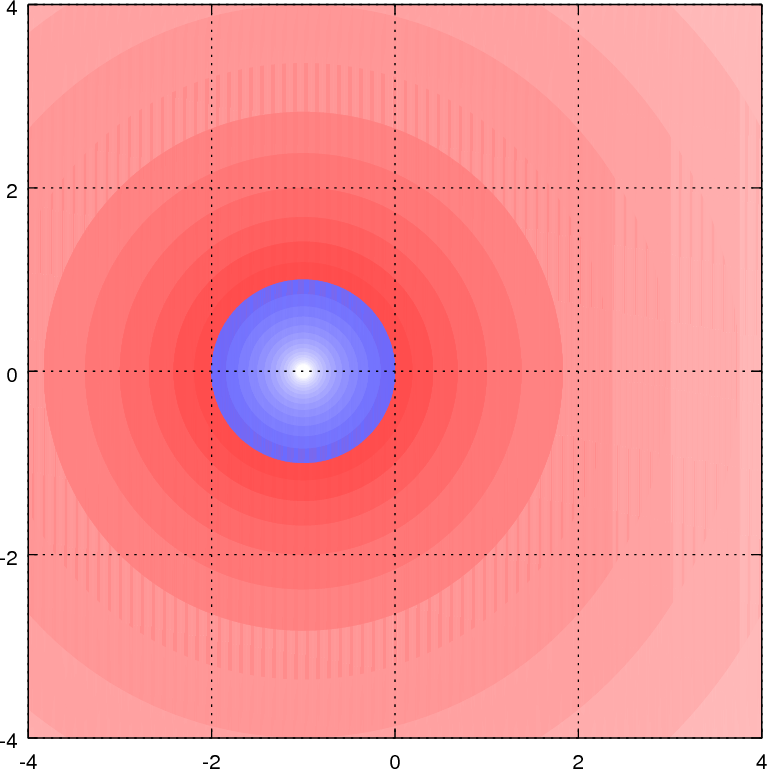
\includegraphics[width=.47\textwidth]{fig/stability-euler}
    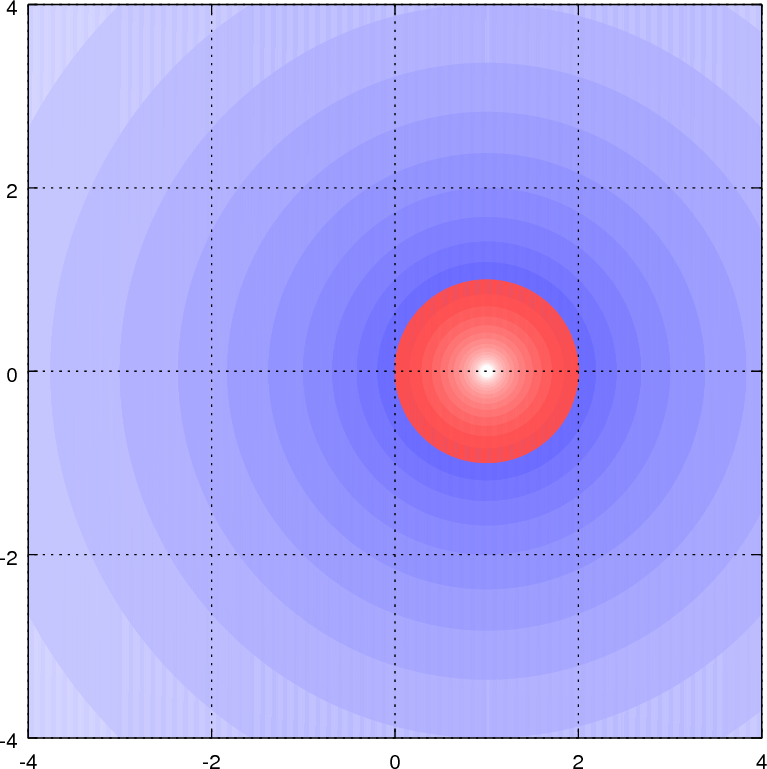
\includegraphics[width=.47\textwidth]{fig/stability-euler2}
  \end{center}
\end{frame}
\frame{\begin{Definition*}{a-stability}{A-stability}
  A method is called \define{A-stable}, if its stability region contains
  the left half-plane of $\C$, hence
  \begin{gather}
    \{ z \in \C | \ Re(z) \le 0 \} \subset S
  \end{gather}
\end{Definition*}

  \begin{Definition*}{a-stability}{A-stability}
  A method is called \define{A-stable}, if its stability region contains
  the left half-plane of $\C$, hence
  \begin{gather}
    \{ z \in \C | \ Re(z) \le 0 \} \subset S
  \end{gather}
\end{Definition*}
}
\frame{\begin{Definition}{b-stability}
  A one-step method is called \define{B-stable}, if for monotonic
  initial value problems $u'=f(u)$ with arbitrary initial value $y_0$
  and $z_0$ there holds:
  \begin{equation}
    | y_1 - z_1 | \le | y_0 - z_0 |
  \end{equation}
  independent of the time step size $h$.
\end{Definition}

  \begin{Definition}{b-stability}
  A one-step method is called \define{B-stable}, if for monotonic
  initial value problems $u'=f(u)$ with arbitrary initial value $y_0$
  and $z_0$ there holds:
  \begin{equation}
    | y_1 - z_1 | \le | y_0 - z_0 |
  \end{equation}
  independent of the time step size $h$.
\end{Definition}
}

\subsection{General Runge-Kutta methods}
\frame{\begin{Definition}{rk}
  A \define{Runge-Kutta method} is a one-step method of the form
  \begin{subequations}
    \label{eq:implicit:1}
    \begin{xalignat}{2}
      \label{eq:implicit:1a}
      \rkg_i &= y_0 + h \sum_{j=1}^{\rks} \rka_{ij} k_j
      & i &= 1,\dots,\rks
      \\
      \label{eq:implicit:1b}
      k_i &= f(t_0+h \rkc_i, \rkg_i)
      & i &= 1,\dots,\rks
      \\
      \label{eq:implicit:1c}
      y_1 &= y_0 + h \sum_{i=1}^{\rks} \rkb_i k_i
    \end{xalignat}
  \end{subequations}
  The method is called
  \begin{description}
  \item[\textbf{ERK}] if $j \ge i\Rightarrow\rka_{ij} = 0$ (``explicit'')
    \index{Runge-Kutta method!explicit (ERK)|textbf}
  \item[\textbf{DIRK}] if $j>i\Rightarrow\rka_{ij} = 0$ (``diagonal implicit'')
    \index{Runge-Kutta method!diagonal implicit (DIRK)|textbf}
    \index{Diagonal implicit (DIRK)}
    \index{DIRK|see{Runge-Kutta method}}
  \item[\textbf{SDIRK}] if DIRK and $\forall i,j: \rka_{ii} =
    \rka_{jj}$ (``singly diagonal implicit'')
    \index{Runge-Kutta method!singly diagonal implicit (SDIRK)|textbf}
    \index{SDIRK|see{Runge-Kutta method}}
  \item[\textbf{IRK}] ``implicit'' in all other cases.
    \index{Runge-Kutta method!implicit (IRK)|textbf}
    \index{IRK|see{Runge-Kutta method}}
  \end{description}
\end{Definition}

%%% Local Variables: 
%%% mode: latex
%%% TeX-master: "../notes"
%%% End: 
}
\frame{% HW2, p. 40
\begin{Lemma}{stability-rk}
  The \putindex{stability function} of an $s$-stage Runge-Kutta method with
  coefficients
  \begin{gather*}
    A=
    \begin{pmatrix}
      \rka_{11} & \cdots & \rka_{1s}
      \\ \vdots & & \vdots \\
      \rka_{s1} & \cdots & \rka_{ss}
    \end{pmatrix},
    b =
    \begin{pmatrix}
      b_1 \\ \vdots \\ b_s
    \end{pmatrix},
  \end{gather*}
  is given by the two expressions
  \begin{gather}
    \label{eq:stability-rk:1}
    R(z) = 1+ z b^T \bigl(\identity-zA\bigr)^{-1}
    \begin{pmatrix}
      1\\\vdots\\1
    \end{pmatrix}
    = \frac{\operatorname{det}\left(\identity-zA+z
        \begin{pmatrix}
          b_1 & \cdots & b_s\\
          \vdots & & \vdots \\
          b_1 & \cdots & b_s
        \end{pmatrix}\right)
}{\operatorname{det}\bigl(\identity-zA\bigr)}
  \end{gather}
\end{Lemma}

%%% Local Variables:
%%% mode: latex
%%% TeX-master: "../notes"
%%% End:
}
\frame{\begin{Example}{stability-examples-rk}
  Stability functions of the modified Euler method, of the classical
  Runge-Kutta method of order 4 and of the Dormand-Prince method of
  order 5 are
  \begin{align*}
    R_2(z) &= 1 + z + \tfrac{z^2}2 \\
    R_4(z) &= 1 + z + \tfrac{z^2}2 + \tfrac{z^3}{6} + \tfrac{z^4}{24}\\
    R_5(z) &= 1 + z + \tfrac{z^2}2 + \tfrac{z^3}{6} + \tfrac{z^4}{24}
             + \tfrac{z^5}{120} + \tfrac{z^6}{600}
  \end{align*}
  respectively. Their stability regions are shown in
  Figure~\ref{fig:implicit:stability-explicit-rk}.
\end{Example}

%%% Local Variables:
%%% mode: latex
%%% TeX-master: "../notes"
%%% End:
}
\begin{frame}
  \frametitle{Stability domains of ERK}
  \begin{tabular}{ccc}
    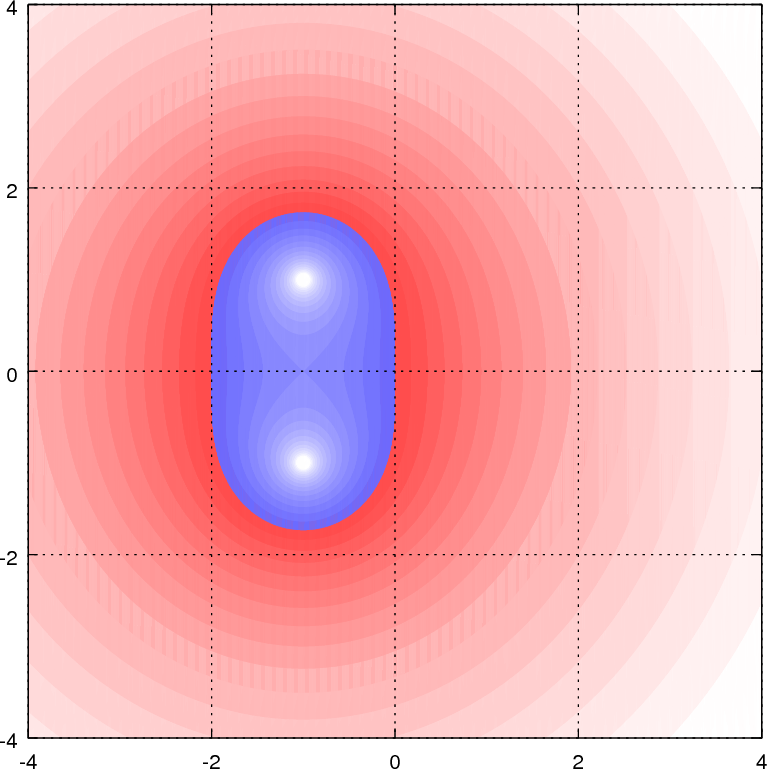
\includegraphics[width=.3\textwidth]{fig/stability-RK2}
    &
    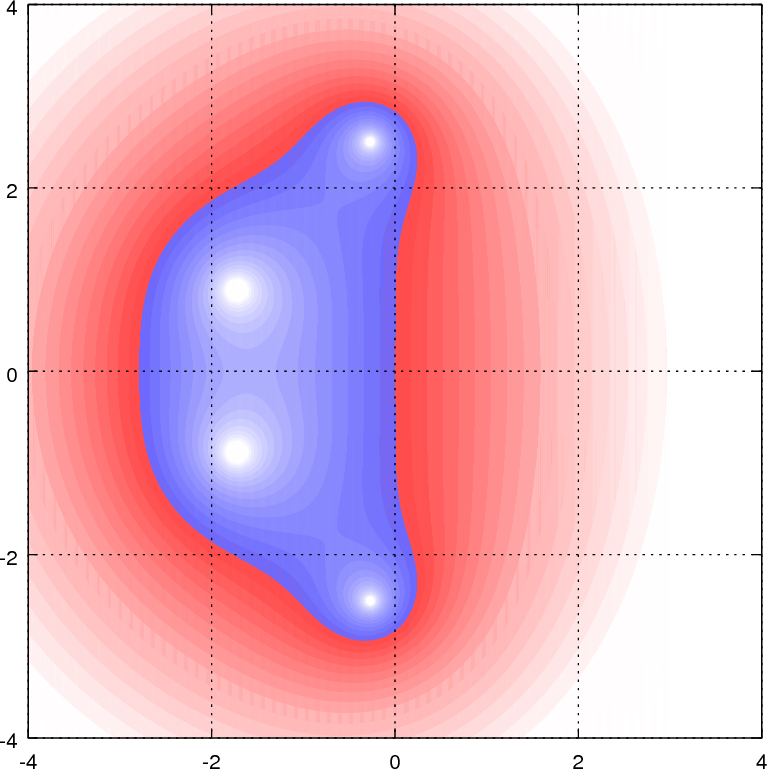
\includegraphics[width=.3\textwidth]{fig/stability-RK4}
    &
    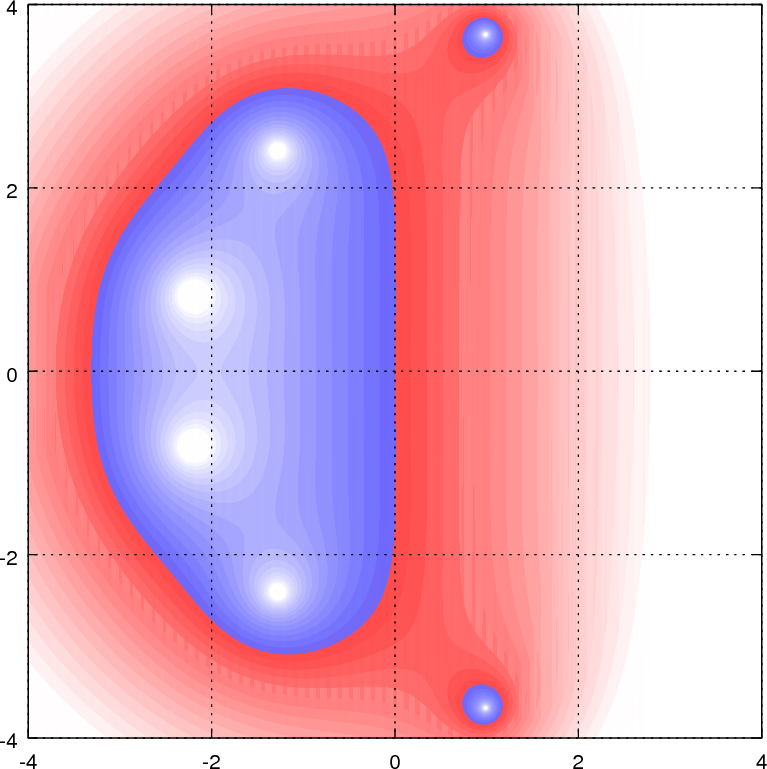
\includegraphics[width=.3\textwidth]{fig/stability-DOPRI5}
    \\
    mod. Euler & RK4 & DOPRI5
  \end{tabular}
\end{frame}
\frame{\begin{Definition}{theta-scheme}
  The $\theta$-scheme is the one-step method, defined for $\theta\in
  [0,1]$ by
  \begin{gather}
    \label{eq:theta:1}
    y_1 = y_0 + h \bigl((1-\theta) f(y_0) + \theta f(y_1)\bigr).
  \end{gather}
  It is an RKM with the Butcher Tableau
  \begin{gather}
    \label{eq:theta:2}
    \begin{array}{c|cc}
      0 & 0 & 0 \\
      1 & 1-\theta & \theta \\\hline
      & 1-\theta & \theta
    \end{array}.
  \end{gather}
  Three special cases are distinguished:
  \begin{center}
  \begin{tabular}{c|l}
    $\theta=0$ & explicit Euler method\\
    $\theta=1$ & implicit Euler method\\
    $\theta=1/2$ & Crank-Nicolson method
  \end{tabular}    
  \end{center}

  Furthermore, we define the variable $\theta$-scheme where $\theta$ is
  of the form
  \begin{gather*}
    \theta = \frac12 + \gamma h.
  \end{gather*}
\end{Definition}
%%% Local Variables:
%%% mode: latex
%%% TeX-master: "../notes"
%%% End:
}
\begin{frame}
  \frametitle{Stability domains of the $\theta$-scheme}
  \begin{center}
    \begin{tabular}{cccc}
      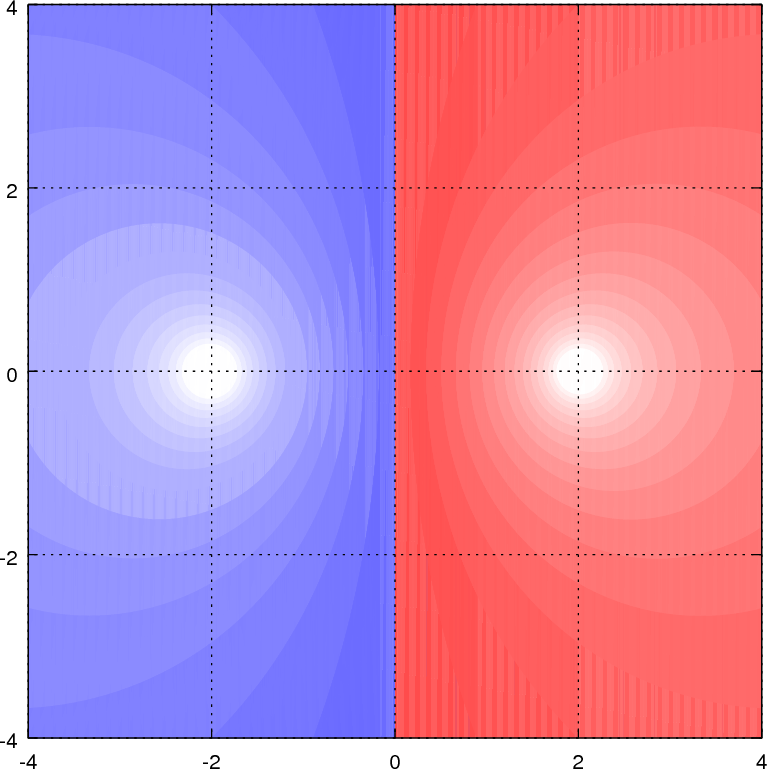
\includegraphics[width=.22\textwidth]{fig/stability-CR}
      &
      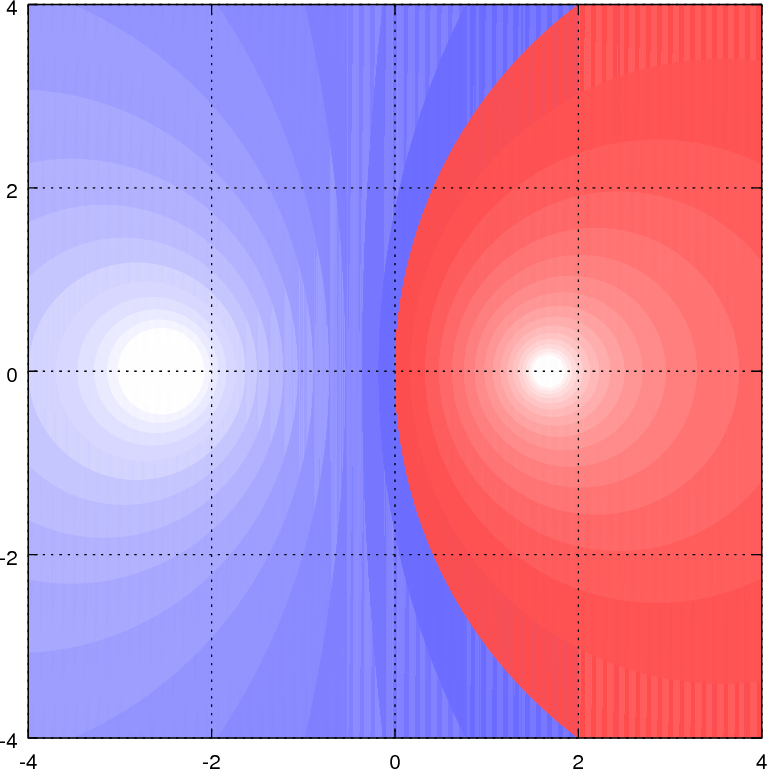
\includegraphics[width=.22\textwidth]{fig/stability-theta6}
      &
      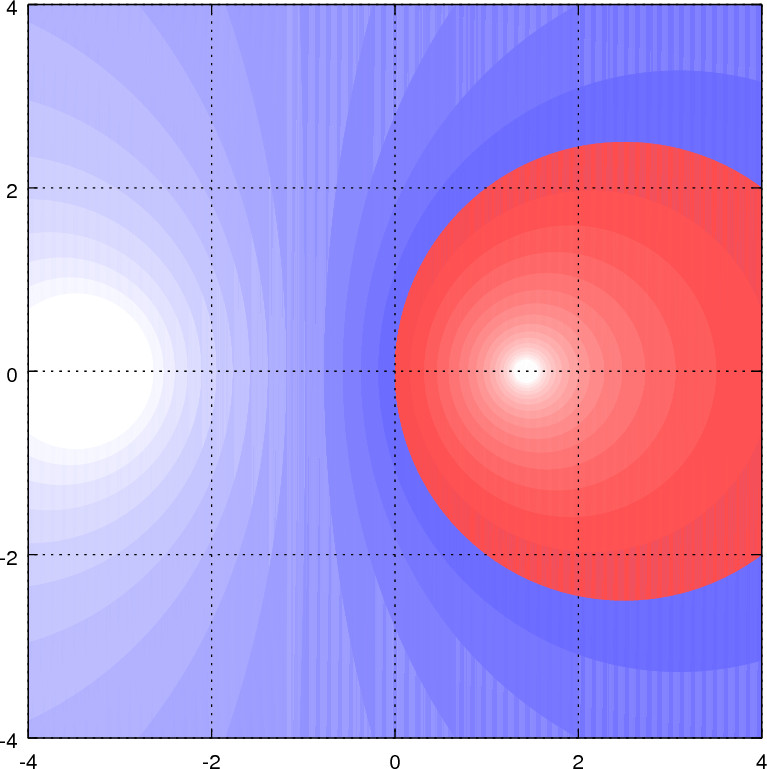
\includegraphics[width=.22\textwidth]{fig/stability-theta7}
      &
      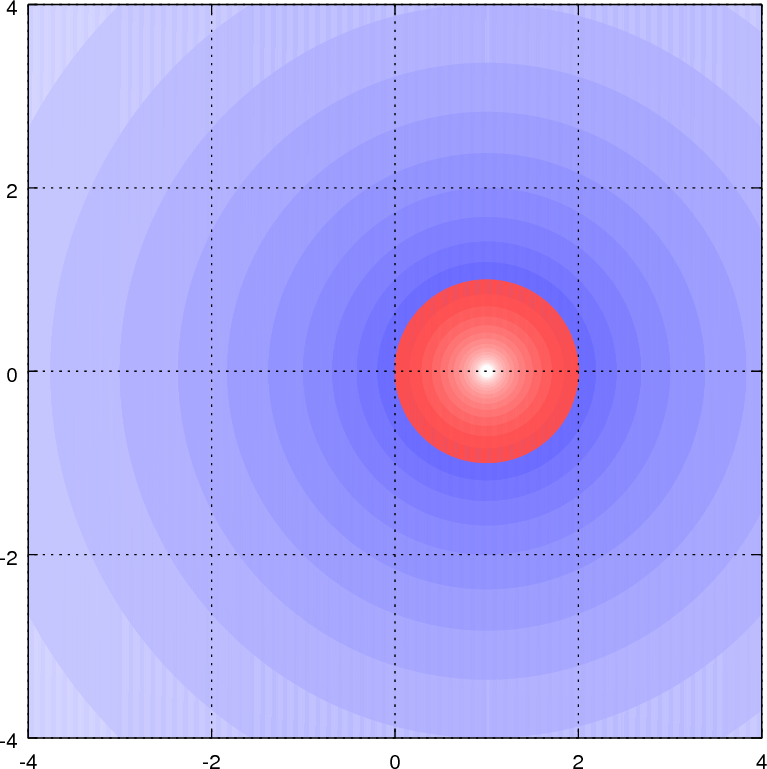
\includegraphics[width=.22\textwidth]{fig/stability-euler2}
      \\
      $\theta= 0.5$
      & $\theta = 0.6$
      & $\theta = 0.7$
      & $\theta = 1.0$
      \\
      Crank-Nicolson &&& impl. Euler
    \end{tabular}
  \end{center}
\end{frame}

\frame{\begin{Lemma}{existence-implicit-1}{Cauchy 1824}
  Let $f:\R\times\C^d\to\C^d$ be continuous and satisfy the Lipschitz
  condition with constant $L$. If
  \begin{gather}
    \label{eq:existence-implicit-1:1}
    hL < \frac1{\max\limits_{i=1,\dots,s} \sum\limits_{j=1}^s \abs{a_{ij}}},
  \end{gather}
  then, for any $y_0$ the Runge-Kutta method~\eqref{eq:implicit:1} has a unique
  solution $y_1$.
\end{Lemma}

%%% Local Variables:
%%% mode: latex
%%% TeX-master: "../notes"
%%% End:
}
\frame{\begin{Lemma}{existence-implicit-2}
  Let $f:\R\times\C^d\to\C^d$ be continuous and satisfy the one-sided Lipschitz
  condition with constant $\nu$. If for $i=1,\dots,s$
  \begin{gather}
    \label{eq:existence-implicit-2:1}
    h\nu < \frac1{a_{ii}}
  \end{gather}
  then, for any $y_0$ the DIRK method~\eqref{eq:implicit:1} has a unique
  solution $y_1$.
\end{Lemma}

%%% Local Variables:
%%% mode: latex
%%% TeX-master: "../notes"
%%% End:
}
\frame{\begin{Theorem}{existence-implicit-3}
  Let be $f$ continuously differentiable and let it satisfy the 
  one-sided Lipschitz condition with constant $\nu$. If the
  Runge-Kutta matrix $A$ is invertible and if there is a vector
  $(d_1,\dots,d_s)$ with positive entries, such that
  \begin{gather}
    \label{eq:implicit:cond}
    h\nu < \frac{\scal(x,A^{-1}x)}{\sum\limits_{i=1}^s d_i x_i^2},
    \quad\forall x\in \R^s,
  \end{gather}
  then the nonlinear system~\ref{eq:implicit:1a} has a solution
  $(\rkg_1,...,\rkg_\rks)$.

\end{Theorem}
%%% Local Variables: 
%%% mode: latex
%%% TeX-master: "../notes"
%%% End: 
}
\frame{\begin{Definition*}{simplifying-conditions}{Simplifying order conditions}
% HNW p. 208
  \index{order condition (IRK)}
  Define the conditions
  \begin{subequations}
    \label{eq:implicit:order}
    \begin{xalignat}{3}
      \label{eq:implicit:8}
      B(\xi):&&
      \sum_{i=1}^s \rkb_i \rkc_i^{q-1} &= \frac1{q}
      &&
      \begin{array}{r@{\,}l}
        q&=1,\ldots,\xi
      \end{array}
      \\
      \label{eq:implicit:9}
      C(\xi):&& \sum_{j=1}^s \rka_{ij} \rkc_j^{q-1} &= \frac{\rkc_i^{q}}{q}
      &&
      \begin{array}{r@{\,}l}
        q&=1,\ldots,\xi\\
        i&=1,\dots,\rks
      \end{array}
      \\
      \label{eq:implicit:11}
      D(\xi):&&
      \sum_{i=1}^s \rkb_i \rka_{ij} \rkc_i^{q-1} &=
      \frac{\rkb_j}{q}(1-\rkc_j^{q})
      &&
      \begin{array}{r@{\,}l}
        q&=1,\ldots,\xi\\
        j&=1,\dots,\rks
      \end{array}
    \end{xalignat}
  \end{subequations}
\end{Definition*}

%%% Local Variables: 
%%% mode: latex
%%% TeX-master: "../notes"
%%% End: 
%}

%\frame{
\begin{Definition*}{simplifying-conditions}{Simplifying order conditions}
% HNW p. 208
  \index{order condition (IRK)}
  Define the conditions
  \begin{subequations}
    \label{eq:implicit:order}
    \begin{xalignat}{3}
      \label{eq:implicit:8}
      B(\xi):&&
      \sum_{i=1}^s \rkb_i \rkc_i^{q-1} &= \frac1{q}
      &&
      \begin{array}{r@{\,}l}
        q&=1,\ldots,\xi
      \end{array}
      \\
      \label{eq:implicit:9}
      C(\xi):&& \sum_{j=1}^s \rka_{ij} \rkc_j^{q-1} &= \frac{\rkc_i^{q}}{q}
      &&
      \begin{array}{r@{\,}l}
        q&=1,\ldots,\xi\\
        i&=1,\dots,\rks
      \end{array}
      \\
      \label{eq:implicit:11}
      D(\xi):&&
      \sum_{i=1}^s \rkb_i \rka_{ij} \rkc_i^{q-1} &=
      \frac{\rkb_j}{q}(1-\rkc_j^{q})
      &&
      \begin{array}{r@{\,}l}
        q&=1,\ldots,\xi\\
        j&=1,\dots,\rks
      \end{array}
    \end{xalignat}
  \end{subequations}
\end{Definition*}

%%% Local Variables: 
%%% mode: latex
%%% TeX-master: "../notes"
%%% End: 
}

\subsection{Methods based on quadrature}
\frame{\begin{Lemma}{gauss-quadrature}
  A Gauß quadrature formula with $n$ points is exact for polynomials
  of degree $2n-1$. A Radau quadrature formula with $n$ points is
  exact for polynomials of degree $2n-2$. A Lobatto quadrature formula
  with $n$ points is exact for polynomials of degree $2n-3$.
\end{Lemma}}
\frame{\begin{Definition}{radau-lobatto-quadrature}
  The \define{Radau quadrature} formulas use one end point of the interval
  $[0,1]$ and the roots of orthogonal polynomials of degree $n-1$ as
  their abscissas. We distinguish left and right Radau quadrature
  formulas, depending on which end is included. \define{Lobatto quadrature}
  formulas use both end points and the roots of a polynomial of degree
  $n-2$. In all three cases, the abscissas are the roots of the polynomials
  \begin{xalignat}2
    \text{Radau}&\text{ left}
    & p_n(x) &= \frac{d^{n-1}}{dx^{n-1}}\bigl(x^n(x-1)^{n-1}\bigr), \\
    \text{Radau}&\text{ right}
    & p_n(x) &= \frac{d^{n-1}}{dx^{n-1}}\bigl(x^{n-1}(x-1)^{n}\bigr), \\
    \text{Lobatto}&
    & p_n(x) &= \frac{d^{n-2}}{dx^{n-2}}\bigl(x^{n-1}(x-1)^{n-1}\bigr).
  \end{xalignat}
\end{Definition}
}
\frame{\begin{Lemma}{gauss-quadrature}
  A Gauß quadrature formula with $n$ points is exact for polynomials
  of degree $2n-1$. A Radau quadrature formula with $n$ points is
  exact for polynomials of degree $2n-2$. A Lobatto quadrature formula
  with $n$ points is exact for polynomials of degree $2n-3$.
\end{Lemma}}
\frame{\begin{Lemma}{collocation}
% HKW p. 212
  A $\rks$-stage collocation method with the points $\rkc_1$
  to $\rkc_\rks$ defines a Runge-Kutta method of
  definition~\ref{definition:rk} with the coefficients $\rkc_i$ and
  \begin{gather}
  \label{eq:implicit:kolkoef}
    \rka_{ij} =  \int_0^{\rkc_i} L_j(t)\, \diffd t,
    \qquad
    \rkb_i =\int_0^1 L_j(t)\, \diffd t.
  \end{gather}
  Here is $L_j(t)$ Lagrange's interpolation polynomial to point $\rkc_j$
  and to the point set $\{\rkc_1,\dots,\rkc_\rks\}$:
  \begin{gather*}
    L_j(t) = \prod_{\substack{k=1\\k\neq j}}^\rks \frac{t-\rkc_k}{\rkc_j-\rkc_k}.
  \end{gather*}
\end{Lemma}

%%% Local Variables: 
%%% mode: latex
%%% TeX-master: "../notes"
%%% End: 
}
\frame{\begin{Lemma}{collocation}
% HKW p. 212
  A $\rks$-stage collocation method with the points $\rkc_1$
  to $\rkc_\rks$ defines a Runge-Kutta method of
  definition~\ref{definition:rk} with the coefficients $\rkc_i$ and
  \begin{gather}
  \label{eq:implicit:kolkoef}
    \rka_{ij} =  \int_0^{\rkc_i} L_j(t)\, \diffd t,
    \qquad
    \rkb_i =\int_0^1 L_j(t)\, \diffd t.
  \end{gather}
  Here is $L_j(t)$ Lagrange's interpolation polynomial to point $\rkc_j$
  and to the point set $\{\rkc_1,\dots,\rkc_\rks\}$:
  \begin{gather*}
    L_j(t) = \prod_{\substack{k=1\\k\neq j}}^\rks \frac{t-\rkc_k}{\rkc_j-\rkc_k}.
  \end{gather*}
\end{Lemma}

%%% Local Variables: 
%%% mode: latex
%%% TeX-master: "../notes"
%%% End: 
}
\frame{\begin{Lemma}{collocation-equivalence}
% HKW p. 212
  An implicit $\rks$-stage Runge-Kutta method of order $\rks$ or
  higher, with pairwise different support points $\rkc_i$ is a
  collocation method if and only if simplifying condition $C(s)$
  in~\eqref{eq:implicit:9} is satisfied. In other words, an
  $\rks$-stage method is a collocation method as soon as all the
  ``quadrature formulas'' involved are of order at least $\rks$.
\end{Lemma}

%%% Local Variables: 
%%% mode: latex
%%% TeX-master: "../notes"
%%% End: 
}
\frame{\begin{Theorem}{collocation-order}
  Consider a collocation method with $s$ pairwise different support
  points $\rkc_i$ and define
  \begin{gather}
    \label{eq:implicit:14}
    \pi(t) = \prod_{i=1}^\rks (t-c_i).  
  \end{gather}
  If $\pi(t)$ is orthogonal on $[0,1]$ to all polynomials of degree
  $r-1$ for $r\le s$, then the collocation
  method~\eqref{eq:implicit:13} is of order $p=s+r$.
\end{Theorem}


%%% Local Variables: 
%%% mode: latex
%%% TeX-master: "../notes"
%%% End: 
}
\frame{\begin{Theorem}{collocation-continuous}
  \index{Runge-Kutta method!continuous} The collocation polynomial
  $y(t)$, defined through an $\rks$-stage collocation method of the
  form~\eqref{eq:implicit:13}, defines a continuous Runge-Kutta method
  of order $s$. This means for the difference of the exact solution
  $u(t)$ of the initial value problem and the collocation polynomial
  $y(t)$ we get the estimate
  \begin{gather}
    \label{eq:implicit:15}
    \abs{u(t)-y(t)} \le C h^{s+1}.
  \end{gather}
  Additionally we obtain for the derivatives of order $k\le s$ the
	estimate
  \begin{gather}
    \label{eq:implicit:16}
    \abs{u^{(k)}(t)-y^{(k)}(t)} \le C h^{s+1-k}.
  \end{gather}
\end{Theorem}
}
\begin{frame}
  \begin{Definition}{gauss-collocation}
  \defindex{collocation method!Gauß} An $\rks$-stage
  \define{Gauß-Collocation method} is a collocation method, where the
  collocation points are the set of $\rks$ Gauß points in the interval
  $[0,1]$, namely the roots of the Legendre polynomial of degree $\rks$.
\end{Definition}

  \begin{block}{2- and 3-point Gauß-Collocation}
  \begin{minipage}[t]{.39\linewidth}
    \begin{gather*}
  \def\arraystretch{1.5}
  \begin{array}{c|cc}  
    \frac{3-\sqrt3}{6} & \frac14 & \frac14-\frac{\sqrt3}{6}
    \\
    \frac{3+\sqrt3}{6} & \frac14+\frac{\sqrt3}{6} & \frac14
    \\\hline
                       & \frac12 & \frac12
  \end{array}
\end{gather*}

%%% Local Variables:
%%% mode: latex
%%% TeX-master: "../notes"
%%% End:

  \end{minipage}
  \begin{minipage}[t]{.55\linewidth}
    \begin{gather*}
  \def\arraystretch{1.5}
  \begin{array}{c|ccc}
    \frac{5-\sqrt{15}}{10}
    & \frac{5}{36}
    & \frac29 - \frac{\sqrt{15}}{15}
    & \frac{5}{36} - \frac{\sqrt{15}}{30}
    \\
    \frac12
    & \frac{5}{36} + \frac{\sqrt{15}}{24}
    & \frac29
    & \frac{5}{36} - \frac{\sqrt{15}}{24}
    \\
    \frac{5+\sqrt{15}}{10}
    & \frac{5}{36} + \frac{\sqrt{15}}{30}
    & \frac29 + \frac{\sqrt{15}}{15}
    & \frac{5}{36}
    \\\hline
    & \frac{5}{18} & \frac49 & \frac{5}{18}
  \end{array}  
\end{gather*}

%%% Local Variables:
%%% mode: latex
%%% TeX-master: "../notes"
%%% End:
      
  \end{minipage}
  \end{block}
\end{frame}
\frame{\begin{Theorem}{gauss-consistency}
  The $\rks$-stage Gauß-collocation method is consistent of order
  $2\rks$ and thus of optimal order.
  
  The $\rks$-stage Radau- and Lobatto-collocation methods are of
  orders $2s-1$ and $2s-2$, respectively.
\end{Theorem}


%%% Local Variables:
%%% mode: latex
%%% TeX-master: "../notes"
%%% End:

\begin{Theorem}{gauss-stability}
% HW p. 181 Example 12.3
  Collocation methods with Gauß-, Radau- and Lobatto-quadrature are
  \putindex{B-stable}. The stability region of Gauß-collocation is
  exactly the left half-plane of $\C$.
\end{Theorem}

%%% Local Variables:
%%% mode: latex
%%% TeX-master: "../notes"
%%% End:
}

\begin{frame}
  \begin{block}{2- and 3-point Radau collocation methods}
  \begin{minipage}[t]{.39\linewidth}
    \begin{gather*}
  \def\arraystretch{1.5}
  \begin{array}{c|cc}  
    \frac13 & \frac{5}{12} & -\frac{1}{12}
    \\
    1 & \frac34 & \frac14
    \\\hline
            & \frac34 & \frac14
  \end{array}
\end{gather*}

%%% Local Variables:
%%% mode: latex
%%% TeX-master: "../notes"
%%% End:

  \end{minipage}
  \begin{minipage}[t]{.55\linewidth}
    \begin{gather*}
  \def\arraystretch{1.5}
  \begin{array}{c|ccc}
    \frac{4-\sqrt{6}}{10}
    & \frac{88-7\sqrt6}{360}
    & \frac{296-169\sqrt6}{1800}
    & \frac{-2+3\sqrt{6}}{225}
    \\
    \frac{4+\sqrt{6}}{10}
    & \frac{296+169\sqrt{6}}{1800}
    & \frac{88+7\sqrt{6}}{360}
    & \frac{-2-3\sqrt6}{225}
    \\
    1
    & \frac{16-\sqrt{6}}{36}
    & \frac{16+\sqrt{6}}{36}
    & \frac19
    \\\hline
    & \frac{16-\sqrt{6}}{36}
    & \frac{16+\sqrt{6}}{36}
    & \frac19
  \end{array}  
\end{gather*}

%%% Local Variables:
%%% mode: latex
%%% TeX-master: "../notes"
%%% End:
      
  \end{minipage}
  \end{block}
\end{frame}

\begin{frame}
  \frametitle{Stability regions of Radau-collocation methods}
    \centering
  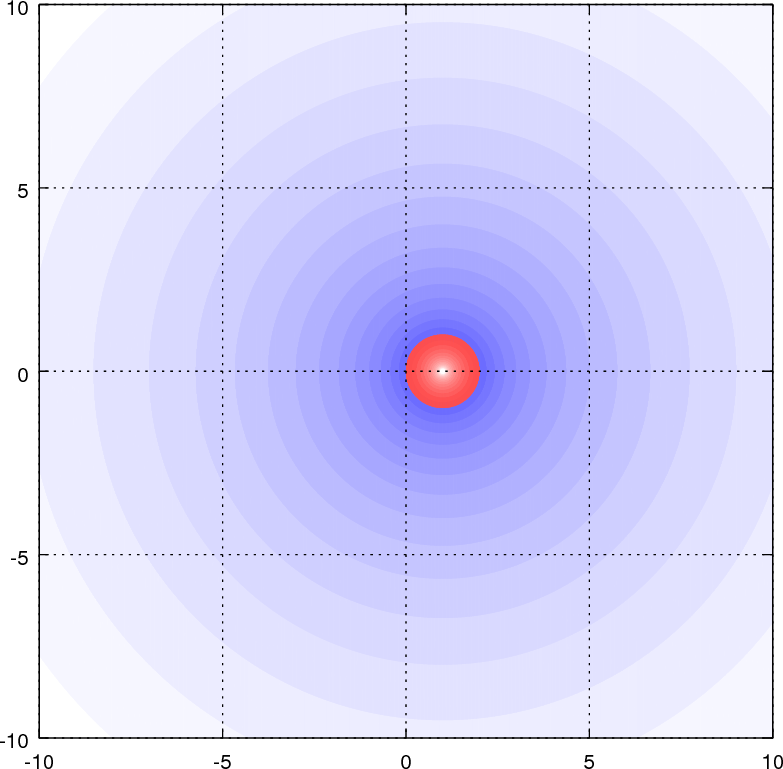
\includegraphics[width=.3\textwidth]{fig/stability-radau1}
  \hfill
  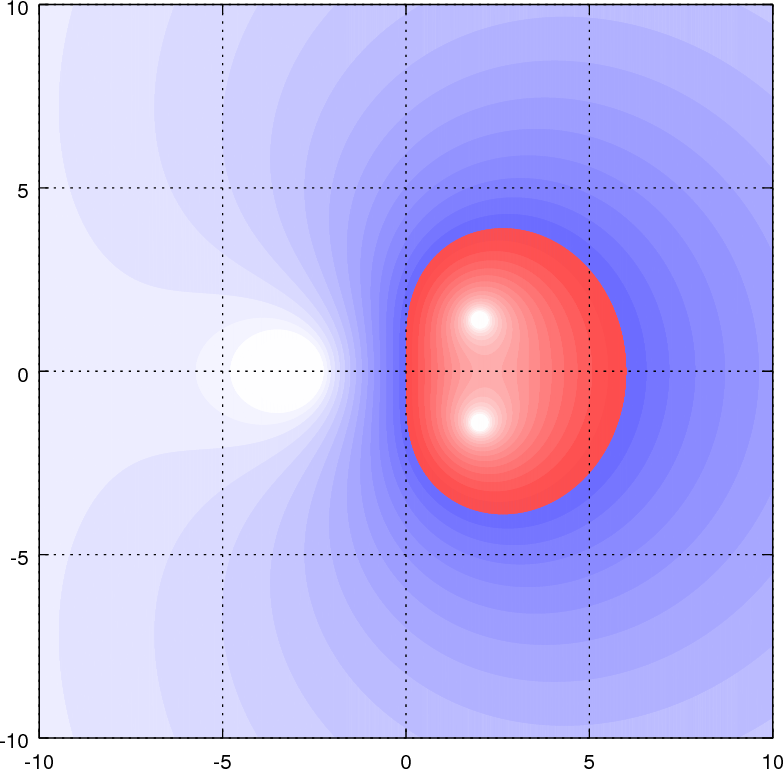
\includegraphics[width=.3\textwidth]{fig/stability-radau2}
  \hfill
  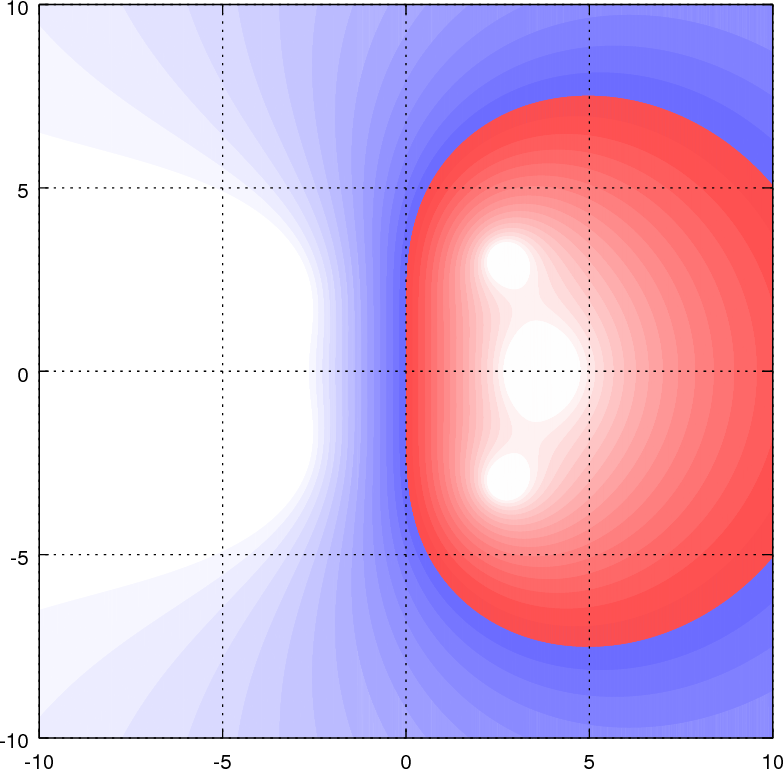
\includegraphics[width=.3\textwidth]{fig/stability-radau3}
\end{frame}

\section{Linear Multi-Step Methods}
\frame{\tableofcontents[currentsection,hideothersubsections]}

\begin{frame}
  \begin{block}{Adams-Moulton methods (implicit)}
  \begin{gather*}
    y_k = y_{k-1} + \sum_{r=0}^\lmms f_{k-r} \int_{t_{k-1}}^{t_k}
    L_r(t) \dt,
  \end{gather*}
    \begin{center}
      \includegraphics[width=.9\textwidth]{fig/adams-moulton.tikz}
    \end{center}
    \begin{align*}
  y_k &= y_{k-1} + h f_k \\
  y_k &= y_{k-1} + \frac12h
        \bigl( f_k + f_{k-1}\bigr)\\
  y_k &= y_{k-1} +
        \frac1{12}h \bigl( 5f_k + 8 f_{k-1} -  f_{k-2}\bigr)\\
  y_k &= y_{k-1} +
        \frac1{24}h \bigl(9f_k+19 f_{k-1}-5 f_{k-2}+ f_{k-3}\bigr)
\end{align*}

%%% Local Variables:
%%% mode: latex
%%% TeX-master: "../notes"
%%% End:
    
  \end{block}
\end{frame}
\begin{frame}
  \begin{block}{Adams-Bashforth methods (explicit)}
  \begin{gather*}
    y_k = y_{k-1} + \sum_{r=1}^\lmms f_{k-r} \int_{t_{k-1}}^{t_k}
    L_r(t) \dt.
  \end{gather*}
    \begin{center}
      \includegraphics[width=.9\textwidth]{fig/adams-bashforth.tikz}
    \end{center}
    \begin{tikzpicture}
  \draw[snake=snake](7,0) -- (8,0);
  \draw(5,0) -- (7,0);
  % \draw(2,0) -- (3,0);
  \draw[dotted](0,0)--(3,0);
  \draw[dashed](3,0)--(5,0);
  
  \draw(8,-.1) --(8,.1) node[anchor=south]{$t_{k}$};
  \draw(7,-.1) node[anchor=north]{$t_{k-1}$} --(7,.1);
  \draw(6,-.1) node[anchor=north]{$t_{k-2}$} --(6,.1);
  \draw(5,-.1) node[anchor=north]{$t_{k-3}$} --(5,.1);
  
  \draw(3,-.1) node[anchor=north]{$t_{k-\lmms}$} --(3,.1);
  % \draw(2,-.1) --(2,.1) node[anchor=south]{$t_{k-\lmms-1}$};
\end{tikzpicture}

  \end{block}
\end{frame}
\begin{frame}
  \begin{block}{Backward Differencing Formulas}
  \begin{gather*}
    y'(t_k) = f(t_k, y_k) = \sum_{r=0}^\lmms y_{k-r} L'_{k-r}(t_k).
  \end{gather*}
    \begin{align*}
  y_k-y_{k-1} &= h f_k \\
  y_k-\tfrac43 y_{k-1} + \tfrac13y_{k-2} &= \tfrac23 h f_k \\
  y_k-\tfrac{18}{11} y_{k-1} + \tfrac{9}{11} y_{k-2} -
  \tfrac{2}{11} y_{k-3}
              &= \tfrac6{11} h f_k \\
  y_k-\tfrac{48}{25} y_{k-1} + \tfrac{36}{25} y_{k-2} -
  \tfrac{16}{25} y_{k-3} + \tfrac{3}{25} y_{k-4}
              &= \tfrac{12}{25} h f_k
\end{align*}

%%% Local Variables:
%%% mode: latex
%%% TeX-master: "../notes"
%%% End:

  \end{block}
\end{frame}

\frame{\chapter{Linear Multistep Methods}


\begin{intro}
  In the previous methods we obtained the value after the next time
  step always by using \emph{one} initial value at the beginning of
  the current time interval, possibly with the
  help of intermediate steps. These methods often are accused to have
  a higher computation time than methods which use several previous
  points, the argument being that function values at these points have
  been computed already. Such methods using values of several time steps in
  the past are called multistep methods. They are constructed such
  that using more steps yields a method of higher order.

  We will begin this chapter by introducing some of the
  formulas. Afterwards, we will study their stability and convergence
  properties.
\end{intro}

\begin{example}[Adams-Moulton formulas]
  \label{ex:lmm:2}  
  \index{Adams-Moulton methods} Basically, there are two construction
  principles for the multistep methods: Quadrature and numerical
  differentiation.  We postpone the latter to example~\ref{ex:lmm:3}
  and deal with the former for now.  As first example we choose the
  class of Adams-Moulton methods for which the integral from point
  $t_{k-1}$ to point $t_{k}$ is approximated by a quadrature of the
  points $t_{k-\lmms}$ to $t_k$, hence
  \begin{gather}
    \label{eq:lmm:16}
    y_k = y_{k-1} + \sum_{r=0}^\lmms f_{k-r} \int_{t_{k-1}}^{t_k}
    L_r(t) \dt,
  \end{gather}
  where $f_j$ denotes the function value $f(t_j, y_j)$ and $L_r(t)$
  the Lagrange interpolation polynomial to point $t_r$ with respect to
  the points $t_{k-\lmms},\dots,t_k$.  This is shown in
  Figure~\ref{fig:lmm:adams-moulton}.
  \begin{figure}[tbp]
    \begin{center}
      \includegraphics[width=.9\textwidth]{fig/adams-moulton.tikz}
    \end{center}
    \caption{The quadrature of Adams-Moulton formulas: the
      integration interval is marked by the wavy line in the end. The support 
			points of the quadrature are stated under the line.}
    \label{fig:lmm:adams-moulton}
  \end{figure}
  Since the integral involves the point being computed itself, these
  methods are implicit. The first of these are
  \begin{align*}
  y_k &= y_{k-1} + h f_k \\
  y_k &= y_{k-1} + \frac12h
        \bigl( f_k + f_{k-1}\bigr)\\
  y_k &= y_{k-1} +
        \frac1{12}h \bigl( 5f_k + 8 f_{k-1} -  f_{k-2}\bigr)\\
  y_k &= y_{k-1} +
        \frac1{24}h \bigl(9f_k+19 f_{k-1}-5 f_{k-2}+ f_{k-3}\bigr)
\end{align*}

%%% Local Variables:
%%% mode: latex
%%% TeX-master: "../notes"
%%% End:
  
\end{example}

\begin{example}[Adams-Bashforth formulas]
  \label{ex:lmm:1}
  \index{Adams-Bashforth methods} With the same principle we obtain
  explicit methods by omitting the point in time $t_k$ in the
  definition of the interpolation polynomial. See
  Figure~\ref{fig:lmm:adams-bashforth}.
  \begin{figure}[tbp]
    \begin{center}
      \includegraphics[width=.9\textwidth]{fig/adams-bashforth.tikz}
    \end{center}
    \caption{The quadrature of Adams-Bashforth formulas: the
      integration interval is marked by the wavy line in the end. The support 
			points of the quadrature are stated under the line.}
    \label{fig:lmm:adams-bashforth}
  \end{figure}
  This yields quadrature formulas of the form
  \begin{gather}
    \label{eq:lmm:17}
    y_k = y_{k-1} + \sum_{r=1}^\lmms f_{k-r} \int_{t_{k-1}}^{t_k}
    L_r(t) \dt.
  \end{gather}
  Again, we list the first few:
  \begin{tikzpicture}
  \draw[snake=snake](7,0) -- (8,0);
  \draw(5,0) -- (7,0);
  % \draw(2,0) -- (3,0);
  \draw[dotted](0,0)--(3,0);
  \draw[dashed](3,0)--(5,0);
  
  \draw(8,-.1) --(8,.1) node[anchor=south]{$t_{k}$};
  \draw(7,-.1) node[anchor=north]{$t_{k-1}$} --(7,.1);
  \draw(6,-.1) node[anchor=north]{$t_{k-2}$} --(6,.1);
  \draw(5,-.1) node[anchor=north]{$t_{k-3}$} --(5,.1);
  
  \draw(3,-.1) node[anchor=north]{$t_{k-\lmms}$} --(3,.1);
  % \draw(2,-.1) --(2,.1) node[anchor=south]{$t_{k-\lmms-1}$};
\end{tikzpicture}

\end{example}

\begin{example}
  \label{ex:lmm:3}
  \index{BDF methods} Backward differencing formulas (BDF) are as well
  based on Lagrange interpolation at the points $t_{k-\lmms}$ to
  $t_k$. In contrast to Adams formulas they do not use quadrature for
  the right hand side, but rather the derivative of the interpolation
  polynomial in the point $t_k$.  Using Lagrange interpolation
  polynomials $L_i(t)$, we let
  \begin{gather*}
    y(t) = \sum_{r=0}^\lmms y_{n-r} L_{n-r}(t),
  \end{gather*}
  where $y_n$ is still to determine. Now we assume that $y$ solves the ODE
  in point $t_n$, hence
  \begin{gather*}
    y'(t_n) = f(t_n, y_n) = \sum_{r=0}^\lmms y_{n-r} L'_{n-r}(t_n).
  \end{gather*}
  This yields the following schemes:
  \begin{align*}
  y_k-y_{k-1} &= h f_k \\
  y_k-\tfrac43 y_{k-1} + \tfrac13y_{k-2} &= \tfrac23 h f_k \\
  y_k-\tfrac{18}{11} y_{k-1} + \tfrac{9}{11} y_{k-2} -
  \tfrac{2}{11} y_{k-3}
              &= \tfrac6{11} h f_k \\
  y_k-\tfrac{48}{25} y_{k-1} + \tfrac{36}{25} y_{k-2} -
  \tfrac{16}{25} y_{k-3} + \tfrac{3}{25} y_{k-4}
              &= \tfrac{12}{25} h f_k
\end{align*}

%%% Local Variables:
%%% mode: latex
%%% TeX-master: "../notes"
%%% End:

  For an example on how to derive these schemes see the appendix.
\end{example}

\begin{remark}
  We know from introduction to numerical analysis, that the numerical
  differentiation and the extrapolation, the evaluation of
  interpolation polynomials outside of the interval which is spanned
  through the interpolation points, are not stable.  Therefore, we
  expect stability problems for the Adams-Bashforth and BDF
  methods. Moreover, we remember that Lagrange interpolation with
  equidistant support points is unstable for a high-degree
  polynomials. Therefore, we also expect that all methods above
  perform well only with moderate order.
\end{remark}

%%%%%%%%%%%%%%%%%%%%%%%%%%%%%%%%%%%%%%%%%%%%%%%%%%%%%%%%%%%%%%%%%%%%%%
%%%%%%%%%%%%%%%%%%%%%%%%%%%%%%%%%%%%%%%%%%%%%%%%%%%%%%%%%%%%%%%%%%%%%%
\section{Definition and consistency of LMM}
%%%%%%%%%%%%%%%%%%%%%%%%%%%%%%%%%%%%%%%%%%%%%%%%%%%%%%%%%%%%%%%%%%%%%%
%%%%%%%%%%%%%%%%%%%%%%%%%%%%%%%%%%%%%%%%%%%%%%%%%%%%%%%%%%%%%%%%%%%%%%

\chapter{Linear Multistep Methods}


\begin{intro}
  In the previous methods we obtained the value after the next time
  step always by using \emph{one} initial value at the beginning of
  the current time interval, possibly with the
  help of intermediate steps. These methods often are accused to have
  a higher computation time than methods which use several previous
  points, the argument being that function values at these points have
  been computed already. Such methods using values of several time steps in
  the past are called multistep methods. They are constructed such
  that using more steps yields a method of higher order.

  We will begin this chapter by introducing some of the
  formulas. Afterwards, we will study their stability and convergence
  properties.
\end{intro}

\begin{example}[Adams-Moulton formulas]
  \label{ex:lmm:2}  
  \index{Adams-Moulton methods} Basically, there are two construction
  principles for the multistep methods: Quadrature and numerical
  differentiation.  We postpone the latter to example~\ref{ex:lmm:3}
  and deal with the former for now.  As first example we choose the
  class of Adams-Moulton methods for which the integral from point
  $t_{k-1}$ to point $t_{k}$ is approximated by a quadrature of the
  points $t_{k-\lmms}$ to $t_k$, hence
  \begin{gather}
    \label{eq:lmm:16}
    y_k = y_{k-1} + \sum_{r=0}^\lmms f_{k-r} \int_{t_{k-1}}^{t_k}
    L_r(t) \dt,
  \end{gather}
  where $f_j$ denotes the function value $f(t_j, y_j)$ and $L_r(t)$
  the Lagrange interpolation polynomial to point $t_r$ with respect to
  the points $t_{k-\lmms},\dots,t_k$.  This is shown in
  Figure~\ref{fig:lmm:adams-moulton}.
  \begin{figure}[tbp]
    \begin{center}
      \includegraphics[width=.9\textwidth]{fig/adams-moulton.tikz}
    \end{center}
    \caption{The quadrature of Adams-Moulton formulas: the
      integration interval is marked by the wavy line in the end. The support 
			points of the quadrature are stated under the line.}
    \label{fig:lmm:adams-moulton}
  \end{figure}
  Since the integral involves the point being computed itself, these
  methods are implicit. The first of these are
  \begin{align*}
  y_k &= y_{k-1} + h f_k \\
  y_k &= y_{k-1} + \frac12h
        \bigl( f_k + f_{k-1}\bigr)\\
  y_k &= y_{k-1} +
        \frac1{12}h \bigl( 5f_k + 8 f_{k-1} -  f_{k-2}\bigr)\\
  y_k &= y_{k-1} +
        \frac1{24}h \bigl(9f_k+19 f_{k-1}-5 f_{k-2}+ f_{k-3}\bigr)
\end{align*}

%%% Local Variables:
%%% mode: latex
%%% TeX-master: "../notes"
%%% End:
  
\end{example}

\begin{example}[Adams-Bashforth formulas]
  \label{ex:lmm:1}
  \index{Adams-Bashforth methods} With the same principle we obtain
  explicit methods by omitting the point in time $t_k$ in the
  definition of the interpolation polynomial. See
  Figure~\ref{fig:lmm:adams-bashforth}.
  \begin{figure}[tbp]
    \begin{center}
      \includegraphics[width=.9\textwidth]{fig/adams-bashforth.tikz}
    \end{center}
    \caption{The quadrature of Adams-Bashforth formulas: the
      integration interval is marked by the wavy line in the end. The support 
			points of the quadrature are stated under the line.}
    \label{fig:lmm:adams-bashforth}
  \end{figure}
  This yields quadrature formulas of the form
  \begin{gather}
    \label{eq:lmm:17}
    y_k = y_{k-1} + \sum_{r=1}^\lmms f_{k-r} \int_{t_{k-1}}^{t_k}
    L_r(t) \dt.
  \end{gather}
  Again, we list the first few:
  \begin{tikzpicture}
  \draw[snake=snake](7,0) -- (8,0);
  \draw(5,0) -- (7,0);
  % \draw(2,0) -- (3,0);
  \draw[dotted](0,0)--(3,0);
  \draw[dashed](3,0)--(5,0);
  
  \draw(8,-.1) --(8,.1) node[anchor=south]{$t_{k}$};
  \draw(7,-.1) node[anchor=north]{$t_{k-1}$} --(7,.1);
  \draw(6,-.1) node[anchor=north]{$t_{k-2}$} --(6,.1);
  \draw(5,-.1) node[anchor=north]{$t_{k-3}$} --(5,.1);
  
  \draw(3,-.1) node[anchor=north]{$t_{k-\lmms}$} --(3,.1);
  % \draw(2,-.1) --(2,.1) node[anchor=south]{$t_{k-\lmms-1}$};
\end{tikzpicture}

\end{example}

\begin{example}
  \label{ex:lmm:3}
  \index{BDF methods} Backward differencing formulas (BDF) are as well
  based on Lagrange interpolation at the points $t_{k-\lmms}$ to
  $t_k$. In contrast to Adams formulas they do not use quadrature for
  the right hand side, but rather the derivative of the interpolation
  polynomial in the point $t_k$.  Using Lagrange interpolation
  polynomials $L_i(t)$, we let
  \begin{gather*}
    y(t) = \sum_{r=0}^\lmms y_{n-r} L_{n-r}(t),
  \end{gather*}
  where $y_n$ is still to determine. Now we assume that $y$ solves the ODE
  in point $t_n$, hence
  \begin{gather*}
    y'(t_n) = f(t_n, y_n) = \sum_{r=0}^\lmms y_{n-r} L'_{n-r}(t_n).
  \end{gather*}
  This yields the following schemes:
  \begin{align*}
  y_k-y_{k-1} &= h f_k \\
  y_k-\tfrac43 y_{k-1} + \tfrac13y_{k-2} &= \tfrac23 h f_k \\
  y_k-\tfrac{18}{11} y_{k-1} + \tfrac{9}{11} y_{k-2} -
  \tfrac{2}{11} y_{k-3}
              &= \tfrac6{11} h f_k \\
  y_k-\tfrac{48}{25} y_{k-1} + \tfrac{36}{25} y_{k-2} -
  \tfrac{16}{25} y_{k-3} + \tfrac{3}{25} y_{k-4}
              &= \tfrac{12}{25} h f_k
\end{align*}

%%% Local Variables:
%%% mode: latex
%%% TeX-master: "../notes"
%%% End:

  For an example on how to derive these schemes see the appendix.
\end{example}

\begin{remark}
  We know from introduction to numerical analysis, that the numerical
  differentiation and the extrapolation, the evaluation of
  interpolation polynomials outside of the interval which is spanned
  through the interpolation points, are not stable.  Therefore, we
  expect stability problems for the Adams-Bashforth and BDF
  methods. Moreover, we remember that Lagrange interpolation with
  equidistant support points is unstable for a high-degree
  polynomials. Therefore, we also expect that all methods above
  perform well only with moderate order.
\end{remark}

%%%%%%%%%%%%%%%%%%%%%%%%%%%%%%%%%%%%%%%%%%%%%%%%%%%%%%%%%%%%%%%%%%%%%%
%%%%%%%%%%%%%%%%%%%%%%%%%%%%%%%%%%%%%%%%%%%%%%%%%%%%%%%%%%%%%%%%%%%%%%
\section{Definition and consistency of LMM}
%%%%%%%%%%%%%%%%%%%%%%%%%%%%%%%%%%%%%%%%%%%%%%%%%%%%%%%%%%%%%%%%%%%%%%
%%%%%%%%%%%%%%%%%%%%%%%%%%%%%%%%%%%%%%%%%%%%%%%%%%%%%%%%%%%%%%%%%%%%%%

\chapter{Linear Multistep Methods}


\begin{intro}
  In the previous methods we obtained the value after the next time
  step always by using \emph{one} initial value at the beginning of
  the current time interval, possibly with the
  help of intermediate steps. These methods often are accused to have
  a higher computation time than methods which use several previous
  points, the argument being that function values at these points have
  been computed already. Such methods using values of several time steps in
  the past are called multistep methods. They are constructed such
  that using more steps yields a method of higher order.

  We will begin this chapter by introducing some of the
  formulas. Afterwards, we will study their stability and convergence
  properties.
\end{intro}

\begin{example}[Adams-Moulton formulas]
  \label{ex:lmm:2}  
  \index{Adams-Moulton methods} Basically, there are two construction
  principles for the multistep methods: Quadrature and numerical
  differentiation.  We postpone the latter to example~\ref{ex:lmm:3}
  and deal with the former for now.  As first example we choose the
  class of Adams-Moulton methods for which the integral from point
  $t_{k-1}$ to point $t_{k}$ is approximated by a quadrature of the
  points $t_{k-\lmms}$ to $t_k$, hence
  \begin{gather}
    \label{eq:lmm:16}
    y_k = y_{k-1} + \sum_{r=0}^\lmms f_{k-r} \int_{t_{k-1}}^{t_k}
    L_r(t) \dt,
  \end{gather}
  where $f_j$ denotes the function value $f(t_j, y_j)$ and $L_r(t)$
  the Lagrange interpolation polynomial to point $t_r$ with respect to
  the points $t_{k-\lmms},\dots,t_k$.  This is shown in
  Figure~\ref{fig:lmm:adams-moulton}.
  \begin{figure}[tbp]
    \begin{center}
      \includegraphics[width=.9\textwidth]{fig/adams-moulton.tikz}
    \end{center}
    \caption{The quadrature of Adams-Moulton formulas: the
      integration interval is marked by the wavy line in the end. The support 
			points of the quadrature are stated under the line.}
    \label{fig:lmm:adams-moulton}
  \end{figure}
  Since the integral involves the point being computed itself, these
  methods are implicit. The first of these are
  \input{definitions/adams-moulton}  
\end{example}

\begin{example}[Adams-Bashforth formulas]
  \label{ex:lmm:1}
  \index{Adams-Bashforth methods} With the same principle we obtain
  explicit methods by omitting the point in time $t_k$ in the
  definition of the interpolation polynomial. See
  Figure~\ref{fig:lmm:adams-bashforth}.
  \begin{figure}[tbp]
    \begin{center}
      \includegraphics[width=.9\textwidth]{fig/adams-bashforth.tikz}
    \end{center}
    \caption{The quadrature of Adams-Bashforth formulas: the
      integration interval is marked by the wavy line in the end. The support 
			points of the quadrature are stated under the line.}
    \label{fig:lmm:adams-bashforth}
  \end{figure}
  This yields quadrature formulas of the form
  \begin{gather}
    \label{eq:lmm:17}
    y_k = y_{k-1} + \sum_{r=1}^\lmms f_{k-r} \int_{t_{k-1}}^{t_k}
    L_r(t) \dt.
  \end{gather}
  Again, we list the first few:
  \input{definitions/adams-bashforth}
\end{example}

\begin{example}
  \label{ex:lmm:3}
  \index{BDF methods} Backward differencing formulas (BDF) are as well
  based on Lagrange interpolation at the points $t_{k-\lmms}$ to
  $t_k$. In contrast to Adams formulas they do not use quadrature for
  the right hand side, but rather the derivative of the interpolation
  polynomial in the point $t_k$.  Using Lagrange interpolation
  polynomials $L_i(t)$, we let
  \begin{gather*}
    y(t) = \sum_{r=0}^\lmms y_{n-r} L_{n-r}(t),
  \end{gather*}
  where $y_n$ is still to determine. Now we assume that $y$ solves the ODE
  in point $t_n$, hence
  \begin{gather*}
    y'(t_n) = f(t_n, y_n) = \sum_{r=0}^\lmms y_{n-r} L'_{n-r}(t_n).
  \end{gather*}
  This yields the following schemes:
  \input{definitions/bdf}
  For an example on how to derive these schemes see the appendix.
\end{example}

\begin{remark}
  We know from introduction to numerical analysis, that the numerical
  differentiation and the extrapolation, the evaluation of
  interpolation polynomials outside of the interval which is spanned
  through the interpolation points, are not stable.  Therefore, we
  expect stability problems for the Adams-Bashforth and BDF
  methods. Moreover, we remember that Lagrange interpolation with
  equidistant support points is unstable for a high-degree
  polynomials. Therefore, we also expect that all methods above
  perform well only with moderate order.
\end{remark}

%%%%%%%%%%%%%%%%%%%%%%%%%%%%%%%%%%%%%%%%%%%%%%%%%%%%%%%%%%%%%%%%%%%%%%
%%%%%%%%%%%%%%%%%%%%%%%%%%%%%%%%%%%%%%%%%%%%%%%%%%%%%%%%%%%%%%%%%%%%%%
\section{Definition and consistency of LMM}
%%%%%%%%%%%%%%%%%%%%%%%%%%%%%%%%%%%%%%%%%%%%%%%%%%%%%%%%%%%%%%%%%%%%%%
%%%%%%%%%%%%%%%%%%%%%%%%%%%%%%%%%%%%%%%%%%%%%%%%%%%%%%%%%%%%%%%%%%%%%%

\input{definitions/lmm}

\begin{remark}
  \index{step size!constant} The LMM was defined for constant step size
  $h$.  In principle it is possible to implement the method with a
  variable step size but we restrict ourselves to the constant case.
  Notes to the step size control can be found later on in this chapter.
\end{remark}

\begin{remark}
  One-step methods were always denoted by describing how to compute
  $y_1$ from $y_0$. Here, the notation becomes more complicated, but
  sometimes we consider only $y_s$ computed from $y_0,\dots,y_{s-1}$
  implying the same rules for $y_k$ computed from
  $y_{k-\lmms},\dots,y_{k-1}$.
\end{remark}
\input{definitions/lmm-errors}

\begin{lemma}
  Consider the differential equation
  \begin{gather*}
    y' = f(t,y) \qquad y(t_0) = y_0
  \end{gather*}
  where f is given continuously differentiable and $y(t)$ is the exact solution.
  For the local error we obtain

  \begin{gather}
    y(t_k)-y_k = \left( \alpha_0 \identity - h\beta_0 \frac{\partial f}{\partial y}(t_k,\eta) \right)^{-1} (L_h u)(t_k).
  \end{gather}

  Here $\eta$ is a value between $y(t_k)$ and $y_k$ if $f$ is a scalar
	function.
  If $f$ is multidimensional, the matrix 
	$\frac{\partial f}{\partial y}(t_k,\eta)$ is the Jacobi matrix, 
	which rows are evaluated at possible places between
	$y(t_k)$ and $y_k$.
\end{lemma}

\begin{proof}
  Considering the local error we can assume exact initial values 
  and therefore we can transform ~\ref{eq:lmm:4} to:
  \begin{gather*}
    \alpha_\lmms y_k + \sum\limits_{r=1}^\lmms \alpha_{\lmms-r} y(t_{k-r})
    = h \left( \beta_\lmms f_k + \sum\limits_{r=1}^\lmms \beta_{\lmms-r} f_{k-r} \right)
  \end{gather*}
  We transform further:
  \begin{multline*}
    \sum\limits_{r=0}^{\lmms} \left( \alpha_r y(t_{k-r})
      - h \beta_r f(t_{k-r},y(t_{k-r})) \right)
    \\
    - \alpha_0 y(t_k) + h \beta_0 f(t_k, y(t_k)) + \alpha_0 y_k
    - h \beta_0 f(t_k,y_k) = 0.
  \end{multline*}
	We now insert ~\ref{eq:lmm:9} which results in
  \begin{gather*}
    (L_h y)(t_k) = \alpha_0 \left( y(t_k) - y_k \right) - h \beta_0 \left( f(t_k,y(t_k)) - f(t_k,y_k) \right)
    \\
    \left( y(t_k) - y_k \right) \left( \alpha_0 \identity - h \beta_0 \frac{f(t_k,y(t_k)) - f(t_k,y_k)}{y(t_k) - y_k} \right)
  \end{gather*}
  By application of the mean value theorem and 
  subsequent transformation we obtain the statement of the theorem.
\end{proof}

      % \cite[Lemma 2.2, p. 369]{HairerNorsettWanner93}

\input{definitions/lmm-consistency}
\input{theorems/lmm-bramble-hilbert}

\begin{proof}
  We start with the Taylor expansion of a solution $u$ of the ODE and
  the corresponding right hand side $f$ for $t_k$, where we insert,
  unlike usual, $f=u'$:
  \begin{alignat*}2
    u(t) &= \sum_{i=0}^p \frac{u^{(i)}(t_k)}{i!}(t-t_k)^i +
    \frac{u^{(p+1)}(\xi)}{(p+1)!}(t-t_k)^{p+1} &=:& \phi(t) + r_u(t)
    \\
    f\bigl(t,u(t)\bigr) &= \sum_{i=1}^p \frac{u^{(i)}(t_k)}{(i-1)!}(t-t_k)^{i-1} +
    \frac{u^{(p+1)}(\xi)}{p!}(t-t_k)^{p} &=:& \phi'(t) + r_f(t),
  \end{alignat*}
  with the Taylor polynomial $\phi(t)$ of degree $p$ and remainder
  $r_u(t)$ and $r_f(t)$. Out of this we calculate:
  \begin{align*}
    L_h u(t_k) =& \sum_{r=0}^\lmms \alpha_{\lmms-r} \phi(t_{k-r}) - h
    \sum_{r=0}^\lmms \beta_{\lmms-r} \phi'(t_{k-r})
    \\
    &+ \sum_{r=0}^\lmms \alpha_{\lmms-r} r_u(t_{k-r}) - h
    \sum_{r=0}^\lmms \beta_{\lmms-r} r_f(t_{k-r}).
  \end{align*}
  Since $t_{k-r}-t_k = r h$, the first row equals a polynomial 
  $\psi(h)$ in $h$ of degree $p$. For the second row we insert the
	reminder estimate $r_u(t) = \mathcal O((t-t_k)^{p+1}) = h
  r_f(t)$ and get:
  \begin{gather}
    \label{eq:lmm:15}
    L_h u(t_k) = L_h \phi(t_k) + \mathcal O(h^{p+1}) = \psi(h) + \mathcal O(h^{p+1}).
  \end{gather}
  According to the definition of the truncation error, this term has to be of
	order $p+1$, such that the method is of order $p$. However it is $\psi$
  of degree $p$. This can only hold true if $L_h\phi=\psi\equiv
  0$. On the other hand $\tau_h(t_k)$ automatically is of order
  $p$. Since $u$ is the solution of an arbitrary right hand side, this
	condition has to be satisfied for all kind of Taylor polynomials $\phi$ 
	of degree $p$.
\end{proof}

\begin{Theorem}{lmm-consistency}
  \index{step size!constant}
  A LMM with constant step size is consistent of order
  $p$ if and only if
    \begin{gather}
      \label{eq:lmm:12}
      \begin{split}
      \sum_{r=0}^\lmms \alpha_{r} &= 0, \\
      \sum_{r=0}^\lmms \bigl(\alpha_{r}r^q - q \beta_{r}
      r^{q-1}\bigr) &= 0,
      \qquad q = 1,\dots,p        
      \end{split}
    \end{gather}
\end{Theorem}


\begin{proof}
  According to lemma~\ref{Lemma:lmm-bramble-hilbert} it is sufficient
  to show that ~\eqref{eq:lmm:12} is equivalent to $L_h \phi_q=0$ for
  polynomials of degree $q\le p$. Due to linearity of the method it
  however is sufficient to show this for a basis of the polynomial
  space of degree $p$.  For that we choose the monomial basis of the
  form
  \begin{gather*}
  \pi_q(t) =
  \left(\frac{t-t_{k-\lmms}}h\right)^q,\qquad q=0,\dots,p.
  \end{gather*}
  For those it holds: $\pi_q(t_{k-r}) = (\lmms-r)^q$. Now we see that
  the first condition is $L_h\pi_0 = 0$ (here is
  $\pi_0'\equiv0$) and the second condition is $L_h\pi_q = 0$.
\end{proof}

\begin{todo}
  Beispiel einer konsistenten LMM, die nicht konvergiert.
\end{todo}

\begin{remark}
  As shown in a homework problem, a consistent LMM is not necessary
  convergent. To understand this behavior and develop criteria for
  convergence we need to diverge into the theory of difference
  equations.
\end{remark}
%%%%%%%%%%%%%%%%%%%%%%%%%%%%%%%%%%%%%%%%%%%%%%%%%%%%%%%%%%%%%%%%%%%%%%
%%%%%%%%%%%%%%%%%%%%%%%%%%%%%%%%%%%%%%%%%%%%%%%%%%%%%%%%%%%%%%%%%%%%%%
\section{Properties of difference equations}
%%%%%%%%%%%%%%%%%%%%%%%%%%%%%%%%%%%%%%%%%%%%%%%%%%%%%%%%%%%%%%%%%%%%%%
%%%%%%%%%%%%%%%%%%%%%%%%%%%%%%%%%%%%%%%%%%%%%%%%%%%%%%%%%%%%%%%%%%%%%%

\begin{intro}
  The stability of LMM can be understood by employing the fairly old
  theory of difference equations. In order to keep the presentation
  simple in this section, we use a different notation for numbering
  indices in the equations. Nevertheless, the coefficients of the
  characteristic polynomial are the same as for LMM.
\end{intro}

\input{definitions/difference-equation}

\begin{Lemma}{lmm:1}
  The solutions of the equation~\eqref{eq:lmm:3} with $y_n\in \R$ or
  $y_n\in \C$ form a vector space of dimension $\lmms$. 
\end{Lemma}

\begin{proof}
  Since the equation~\eqref{eq:lmm:3} is linear and homogeneous, it is
  obvious that if two sequences of solutions $\{y^{(1)}\}$ and
  $\{y^{(2)}\}$ satisfy the equation, sums of multiples of them
  satisfy it too.

  As soon as the initial values $y_0$ to $y_{\lmms-1}$ are chosen, all
  other sequence members are uniquely defined.  Moreover it holds
  \begin{gather*}
    y_0=y_1=\dots=y_{\lmms-1}=0
    \quad\Longrightarrow\quad
    y_n = 0, \;n \ge 0.
  \end{gather*}
  Therefore it is sufficient to consider the first $\lmms$ values.  If
  they are linear independent, then the overall sequences are and vice
  versa. Thus, the initial values form a $\lmms$
  dimensional vector space.
\end{proof}

\input{theorems/difference-equation-solutions}

\begin{proof}
  Inserting the solution $y_n = \xi^n$ into the difference equation
  results in
  \begin{gather*}
    \sum_{r=0}^\lmms \alpha_{r} \xi^{n+r} = \xi^{n}
    \sum_{r=0}^\lmms \alpha_{r} \xi^{r}
    = \xi^{n} \chi(\xi) = 0.
  \end{gather*}
\end{proof}

\input{theorems/difference-equation-basis}

\begin{proof}
  First we observe that the sum of the multiplicities of the roots
  results in the degree of the polynomial:
  \begin{gather*}
    \lmms = \sum_{i=1}^\iota \nu_i.
  \end{gather*}
  Moreover we know because of Lemma~\ref{Lemma:lmm:1}, that $\lmms$ is
  the dimension of the solution space. We show that the sequences
  $\{y^{(i,k)}_n\}$ are linear independent. This is clear for
  sequences of different index $i$. It is also clear for different roots,
  because for $n\to\infty$ the exponential function nullifies the
  influence of the polynomials.
  
  It remains to show that the sequences $\{y^{(i,k)}_n\}$ in fact are
  solutions of the difference equations.  For $k=0$ we have proven
  this already in lemma~\ref{Lemma:difference-equation-solutions}.  We proof the fact here for
  $k=2$ and for a double zero $\xi_i$; the principle for higher order
  roots should be clear then.  Equation~\eqref{eq:lmm:3} applied to
  the sequence $\{n \xi_i^n\}$ results in
  \begin{align*}
    \sum_{r=0}^{\lmms} \alpha_r (n+r) \xi_i^{n+r}
    &= n \xi_i^n \sum_{r=0}^{\lmms} \alpha_r \xi_i^{r}
    + \xi_i^{n+1} \sum_{r=1}^{\lmms} \alpha_r r \xi_i^{r-1}
    \\
    &= n \xi_i^n \rho(\xi_i) + \xi_i^{n+1} \rho'(\xi_i) = 0.
  \end{align*}
  Here the term with $\alpha_0$ vanishes, because it is multiplied
  with $r=0$. $\rho(\xi_i) = \rho'(\xi_i) = 0$ because $\xi_i$ is a
  multiple root.
\end{proof}

\input{theorems/root-test}

\begin{proof}
  According to theorem~\ref{Theorem:difference-equation-basis} we can write all solutions
  as linear combinations of the sequences $y^{(i,k)}$ in
  equation~\eqref{eq:lmm:6}. Therefore,
  \begin{enumerate}
  \item all solutions to $|\xi_i|<1$ for $n\to\infty$ converge to zero
  \item all solutions to $|\xi_i|>1$ for $n\to\infty$ divergence to infinity
  \item all solutions to $|\xi_i|=1$ for $n\to\infty$ stay bounded 
	if and only if $\xi_i$ is simple.
  \end{enumerate}
  This proves the statement of the theorem.
\end{proof}

%%%%%%%%%%%%%%%%%%%%%%%%%%%%%%%%%%%%%%%%%%%%%%%%%%%%%%%%%%%%%%%%%%%%%%
%%%%%%%%%%%%%%%%%%%%%%%%%%%%%%%%%%%%%%%%%%%%%%%%%%%%%%%%%%%%%%%%%%%%%%
\section{Stability and convergence}
%%%%%%%%%%%%%%%%%%%%%%%%%%%%%%%%%%%%%%%%%%%%%%%%%%%%%%%%%%%%%%%%%%%%%%
%%%%%%%%%%%%%%%%%%%%%%%%%%%%%%%%%%%%%%%%%%%%%%%%%%%%%%%%%%%%%%%%%%%%%%

\begin{remark}
  In contrast to one-step methods the convergence of multistep methods
  follows not directly from the consistency of the method, if the
  right hand side of the differential equation satisfies the Lipschitz
  condition~\eqref{eq:IVP:1}.  Analog to the A-stability we will
  discuss this by means of a simple model problem and we will deduce
  stability conditions.
\end{remark}

\begin{remark}
  In the following we investigate the solution to a fixed point in time
  $t$ with a shrinking step size $h$. Therefore we choose $n$
  steps of step size $h = t/n$ and let $n$ go towards infinity.
\end{remark}

\input{definitions/lmm-stability}
\input{theorems/lmm-stability}

\begin{proof}
  The application of the LMM to the equation~\eqref{eq:lmm:1} results
  in the difference equation
  \begin{gather*}
    \sum_{r=0}^{\lmms} \alpha_{\lmms-r} y_{n-r} = 0.
  \end{gather*}
  Now we have to proof that the solutions for fixed $t = h n$ stay
  bounded if $h\to 0$. But we also see that the upper equation does
  not contain $h$. Therefore we have to examine, if the solutions
  $y_n$ stay bounded for $n\to \infty$.  By resorting the summation we
  obtain a difference equation of the form~\eqref{eq:lmm:3}. Due to
  corollary~\ref{Corollary:root-test} it follows the statement of the theorem.
\end{proof}

\begin{Corollary}{adams-stability}
  Adams-Bashforth and Adams-Moulton methods are stable.
\end{Corollary}

\begin{proof}
  For all of these methods the first generating polynomial is $\rho(x)
  = x^\lmms-x^{\lmms-1}$. It has the simple root $\xi_1 = 1$ and the
  $\lmms-1$-fold root 0.
\end{proof}

\begin{Theorem}{BDF-stability}
  The BDF methods are stable for $\lmms \le 6$ and not
  stable for $\lmms \ge 7$.
\end{Theorem}

\input{definitions/lmm-convergence}
\input{theorems/lmm-one-step}

\begin{proof}
  From the general form of LMM we
  obtain
  \begin{gather*}
    \frac1{\alpha_s} \sum_{r=0}^\lmms \alpha_{\lmms-r} y_{k-r}
    = \frac{h}{\alpha_s} \sum_{r=0}^{\lmms-1} \beta_{\lmms-r} f_{k-r}
    + \beta_s f_k.
  \end{gather*}
  We rewrite this to
  \begin{gather*}
    y_k = -\sum_{r=1}^{\lmms} \alpha'_{\lmms-r} y_{k-r} +
    h\psi_h(t_{k-1}, Y_{k-1}),
  \end{gather*}
  where we implicitly enter this formula as value for $y_k$ in the
  computation of $f_k$. It remains to realize that this is the first
  set of $d$ equations in~\eqref{eq:lmm-one-step:1}, and that the
  remaining ones are just shifting $y_i$ to $y_{i+1}$.
\end{proof}

\input{theorems/lmm-one-consistency}

\begin{proof}
  The first component of $Y_k - \widehat Y_k$ is the local error of
  step $k$, which is of order $h^{p+1}$ by the assumption. The other
  components vanish by the definition of the method.
\end{proof}

\input{theorems/lmm-one-stability}

\begin{proof}
  We notice that $\widehat\rho(x) = \sum \alpha'_{s-r} x^r$ is the
  characteristic polynomial of the matrix $A$ and thus its eigenvalues
  are the roots of $\widehat\rho(x)$, which has the same roots as the
  generating polynomial $\rho(x)$. By the root test, we know that
  simple roots, which correspond to irreducible blocks of dimension
  one have maximal modulus one. Furthermore, every Jordan block of
  dimension greater than one corresponds to a multiple root, which by
  assumption has modulus strictly less than one. It is easy to see
  that such a block admits a modified canonical form
  \begin{gather*}
    J_i =
    \begin{pmatrix}
      \lambda_i & 1- \abs{\lambda_i}\\
        & \lambda_i &\ddots\\
          &&\ddots & 1- \abs{\lambda_i}\\
            &&&\lambda_i
    \end{pmatrix}.
  \end{gather*}
  Thus, the canonical form $J = T^{-1}AT$ has norm $\norm{J}_{\infty}
  \le 1$. If we define the norm
  \begin{gather*}
    \norm{x} = \norm{(T^{-1}\otimes \identity)x}_\infty,
  \end{gather*}
  we obtain the result by
  \begin{multline*}
    \norm{(A\otimes \identity)x}
    = \norm{(T^{-1}\otimes \identity)(A\otimes \identity)x}_\infty
    = \norm{(J\otimes \identity)(T^{-1}\otimes \identity)x}_\infty
    \\
    \le \norm{(T^{-1}\otimes \identity)x}_\infty
    = \norm{x}.
  \end{multline*}
\end{proof}

\input{theorems/lmm-convergence}

\begin{proof}
  We reduce the proof to convergence of a one-step method with
  \begin{gather}
    \label{eq:lmm:18}
    Y_k = G(Y_{k-1}) =  (A\otimes \identity) Y_{k-1} + h \verfahren_h(t_{k-1}, Y_{k-1}).
  \end{gather}
  Let $Y_{k-1}$ and $Z_{k-1}$ be two initial values for the interval $I_k$.
  By the previous lemma, we have in the norm defined there, for
  sufficiently small $h$, and assuming a Lipschitz constant $L_h$ for
  $\verfahren_h$ :
  \begin{gather}
    \label{eq:lmm:19}
    \norm{G(Y_{k-1})-G(Z_{k-1})} \le (1+h L_h) \norm{Y_{k-1}-Z_{k-1}}.
  \end{gather}
  Thus, the local error $\eta_k = U_k - \widehat Y_k$ at step $k$, which by
  Lemma~\ref{Lemma:lmm-one-consistency} is bounded by $M h^{p+1}$, accumulates
  until step $n$ at most to $h^{p+1}(1_h L_h)^{n-k}$.

  We have:
  \begin{align*}
    \norm{U_1 - Y_1} &\le (1+h L_h)\norm{U_0-y_0} + M h^{p+1} \\
    \norm{U_2 - Y_2} &\le (1+h L_h)^2\norm{U_0-y_0} +  M h^{p+1} \bigl(1+ (1+h L_h)\bigr)\\
    \norm{U_3 - Y_3} &\le (1+h L_h)^3\norm{U_0-y_0} +  M h^{p+1} \Bigl(\bigl(1+ (1+h L_h)+ (1+h L_h)^2\bigr)\Bigr)\\
    \norm{U_n-Y_n} &\le e^{n h L_h}\norm{U_0-Y_0} +
    \frac{M h^p}{L_h}\bigl(e^{n h L_h} - 1\bigr).
  \end{align*}
\end{proof}

\subsection{Starting procedures}

\begin{intro}
In contrast to one-step methods, where the numerical solution is obtained 
solely from the differential equation and the initial value, multistep 
methods require more than one start value. An LMM with $s$ steps requires $s$ 
known start values $y_{k-s}, \dots, y_{k-1}$. Mostly, they are not provided 
by the IVP itself. Thus, general LMM decompose into two parts: 
\begin{itemize}
\item a \emph{starting phase} where the start values are computed in a 
suitable way and
\item a \emph{run phase} where the LMM is executed. 
\end{itemize}
It is crucial that the method of the starting phase provides a suitable order 
corresponding to the LMM of the run phase, recall Definition 
\ref{Definition:lmm-convergence}. Moreover, it should have analog properties to 
the LMM, like explicit/implicit or applicability to stiff problems. 
% We now consider different starting procedures for an implicit LMM with 
% convergence order $p$. According to Definition \ref{Definition:lmm-convergence} 
% the starting values are required to have the same convergence order. 
Possible choices for the starting phase include multistep methods with variable 
order and one-step methods.  
\end{intro}

\begin{example}[Self starter]
A 2-step BDF method requires $y_0$ and $y_1$ to be known. $y_0$ is given by the 
initial value while $y_1$ is unknown so far. To guarantee that the method has 
order 2, $y_1$ needs to be locally of order 2 at least
\begin{align}\label{eq:lmm_1BDFstarter}
|u(t_1)-y_1| \leq c_0 h^2.
\end{align}
This is ensured, for example, by one step of the 1-step BDF method.

However, starting an LMM with $s>2$ steps by a first-order method and then 
successively increasing the order until $s$ is reached does not provide the 
desired global order. That is due to the fact that the first step limits  
the overall convergence order to 2, compare \eqref{eq:lmm_1BDFstarter}. 
Nevertheless, self starters are often used in practice. 
\end{example}
% In this case local 
% error estimates are used to bound the errors of the starting values and all 
% approximations of the run phase by reducing the step sizes, 
% %. Moreover, also in 
% %the run phase the step sizes are controlled using local error estimates, 
% see the  
% discussion on step size control in Section \ref{section:step_size_control}. 


\begin{example}[Runge-Kutta starter]
\label{Example:RKstarter}
One can use Runge-Kutta methods to start LMM. Since only a fixed
number of starting steps are performed, the local order of the
Runge-Kutta approximation is crucial.  For an implicit LMM with
convergence order $p$ and stepsize $h$ one could use an RK method with
consistency order $p-1$ with the same stepsize $h$.

Consider a 3-step BDF method. Thus, beside $y_0$, we need start values 
$y_1, y_2$ with errors less than $c_0 h^3$. They can be computed by RK methods 
of consistency order $2$, for example by two steps of the 1-stage Gau\ss \ 
collocation method with step size $h$ since it has consistency order $2s=2$, 
see theorem \ref{Theorem:gauss-consistency}.
\end{example}




\begin{example}[Continuous Runge-Kutta starter]
  Another option is to use continuous Runge-Kutta methods and to
  evaluate the continuous approximation to obtain the required
  starting values.

  In constrast to Example \ref{Example:RKstarter} one could also use
  the continuous polynomial approximation of Gau\ss \ collocation to
  start a 3-step BDF method. One step with step size $2h$ of a 2-stage
  Gau\ss \ collocation method would give a polynomial of degree $2$
  which is then evaluated in $t_1=t_0+h$ and $t_2=t_1+h$ to obtain
  $y_1, y_2$. According to Theorem
  \ref{Theorem:collocation-continuous} $y_1, y_2$ have the appropriate
  order.
\end{example}

\begin{remark}
  In practice not the order of a procedure is crucial but rather the
  fact that the errors of all approximations (the start values and all
  approximations of the run phase) are bounded by the user-given
  tolerance, compare Section \ref{section:step_size_control}. Thus,
  the step sizes of all steps are controlled using local error
  estimates. Hence, self starting procedures usually start with very
  small step sizes and increase them successively. Due to their higher
  orders RK starters usually are allowed to use moderate step sizes in
  the beginning. Generally, LMM are applied with variable step sizes
  and orders in practice (see e.g. Exercise 7.2).
\end{remark}



%%%%%%%%%%%%%%%%%%%%%%%%%%%%%%%%%%%%%%%%%%%%%%%%%%%%%%%%%%%%%%%%%%%%%%
%%%%%%%%%%%%%%%%%%%%%%%%%%%%%%%%%%%%%%%%%%%%%%%%%%%%%%%%%%%%%%%%%%%%%%
\section{LMM and stiff problems}
%%%%%%%%%%%%%%%%%%%%%%%%%%%%%%%%%%%%%%%%%%%%%%%%%%%%%%%%%%%%%%%%%%%%%%
%%%%%%%%%%%%%%%%%%%%%%%%%%%%%%%%%%%%%%%%%%%%%%%%%%%%%%%%%%%%%%%%%%%%%%

\begin{Definition*}{lmm-stability-region}{A-stability of LMM}
  \index{stability region!of a LMM}
  The linear model difference equation
  \begin{gather}
    \label{eq:lmm:7}
    \sum_{r=0}^{\lmms} \bigl(\alpha_{\lmms-r} - z \beta_{\lmms-r}) y_{n-r} = 0.
  \end{gather}
  is obtained by applying an LMM to the model equation
  $u' = \lambda u$ and inserting $z=h\lambda$.

  The \define{stability region} of an LMM is the set of points $z\in \C$,
  for which all solution sequences $\{y_n\}$ of the equation~\eqref{eq:lmm:7}
  stay bounded for $n\to\infty$. An LMM is called \define{A-stable}, if the 
  stability region contains the left half-plane of $\C$.
\end{Definition*}


\begin{Definition}{lmm-stability-polynomial}
  The stability polynomial of an LMM is obtained by inserting
  $y_n = x^n$ into the linear model difference equation to obtain
  \begin{gather}
    \label{eq:lmm:8}
    r_z(x) = \sum_{r=0}^{\lmms} \bigl(\alpha_{\lmms-r} - z \beta_{\lmms-r})
    x^{\lmms-r}.
  \end{gather}
\end{Definition}

\begin{remark}
  Instead of the simple amplification function $r(z)$ of the one-step
  methods, we get here a function of two variables.  The point $z$ for
  which we want to show stability and the artificial variable $x$ from
  the analysis of the method.
\end{remark}

\begin{Lemma}{lmm-stability}
  Let $\{\xi_1(z),\dots,\xi_\lmms(z)\}$ be the set of roots of the
  stability polynomial $r_z(x)$ as functions of $z$.
  A point $z\in \C$ is in the stability region of a LMM, if these
  roots satisfy the root test in corollary~\ref{Corollary:root-test}.
\end{Lemma}

\begin{proof}
  The proof is analog to theorem~\ref{Theorem:lmm-stability}.
\end{proof}

\begin{Theorem*}{dahlquist2}{2nd Dahlquist barrier}
  \defindex{Dahlquist barrier (second)} There is no A-stable LMM of
  order $p>2$. Among the A-stable LMM of order 2, the trapezoidal rule
  (Crank-Nicolson) has the smallest error constant.
\end{Theorem*}

\subsection{Relaxed A-stability}

\begin{intro}
  Motivated by the fact that there are no higher order A-stable LMM
  and by highly dissipative problems, people have introduced relaxed
  concepts of A-stability.
\end{intro}

\input{definitions/aa-stability}

\begin{remark}
  The introduction of the A(0)-stability is motivated by linear
  systems of the form $u'=-Au$ with symmetric, positive definite
  matrix $A$. In fact one requires there only stability on the real
  axis because all eigenvalues are real. Thus, any positive angle
  $\alpha$ is sufficient.
  
  Similarly A($\alpha$)-stable LMM are suitable for linear problems in
  which high frequently vibration ($\Im\lambda$ large) decay fast
  ($-\Re\lambda$ large).

  In all cases one observes corresponding properties of the Jacobian
  matrix $\partial_u f$ for the application of nonlinear problems.
\end{remark}

\begin{example}
  The stability regions of the stable BDF methods are in
  Figure~\ref{fig:bdf-stability}. The corresponding values for
  A($\alpha$)-stability and stiff stability are in Table  
\ref{tab:bdf-stability}.
\end{example}
\begin{figure}[tp]
  \centering
  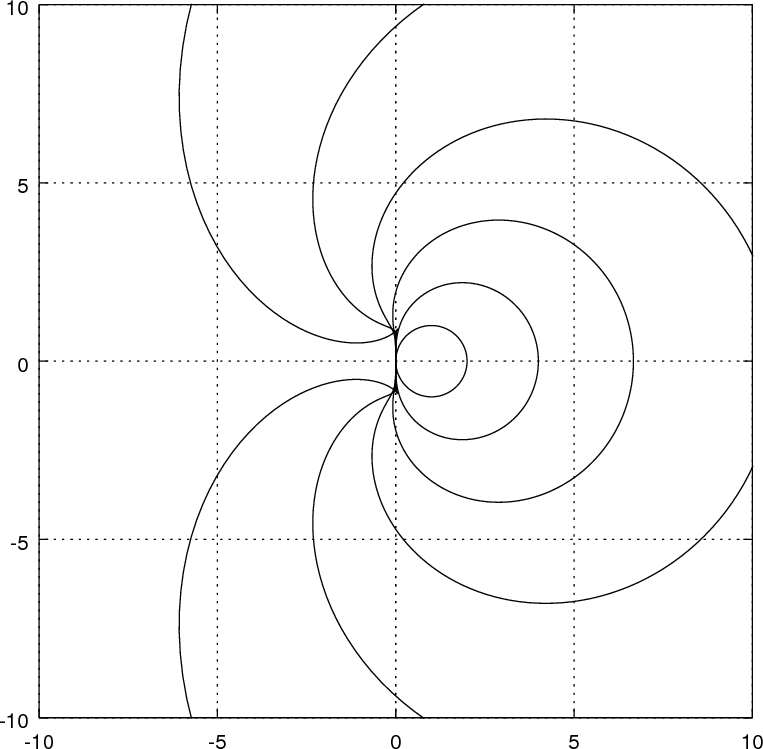
\includegraphics[width=.45\textwidth]{fig/stability-bdf.png}
  \hfill
  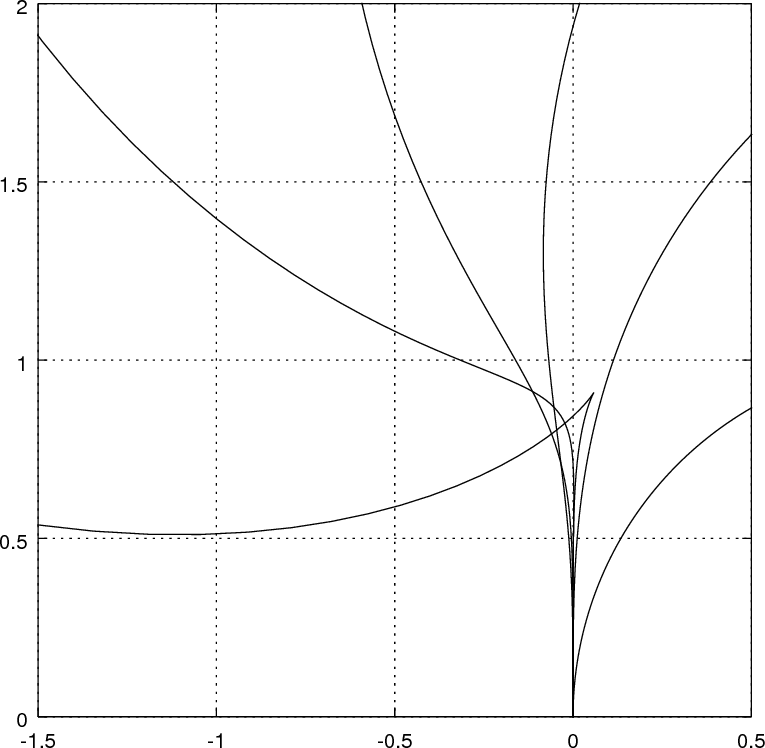
\includegraphics[width=.45\textwidth]{fig/stability-bdf-zoom.png}
  \caption{Boundaries of stability regions of BDF1 to BDF6. Unstable
    region right of the origin. Zoom on the right}
  \label{fig:bdf-stability}
\end{figure}
\begin{table}[tp]
  \centering
  \begin{tabular}{c|cccccc}
    $k$ & 1 & 2 & 3 & 4 & 5 & 6 \\\hline
    $\alpha$ & 90$^\circ$ & 90$^\circ$& 86.03$^\circ$
                    & 73.35$^\circ$& 51.84$^\circ$
                            & 17.84$^\circ$ \\
    $D$ & 0 & 0 & 0.083& 0.667& 2.327& 6.075
  \end{tabular}
  \caption{Values for A($\alpha$)- and stiff stability for BDF methods
    of order $k$.}
  \label{tab:bdf-stability}
\end{table}

%%%%%%%%%%%%%%%%%%%%%%%%%%%%%%%%%%%%%%%%%%%%%%%%%%%%%%%%%%%%%%%%%%%%%%
\section{Predictor-corrector schemes}

\begin{Definition*}{predictor-corrector}{Predictor-corrector methods}
  Assume a pair of time stepping schemes, one explicit, one implicit,
  \begin{align*}
    \hat y_{k} &= \hat \verfahren_p(y_{k-1}) \\
    y_k &= \verfahren_c(y_{k-1},y_{k}),
  \end{align*}
  we can use $\hat y_k$ as initial value for the Newton iteration for
  $y_k$. In an extreme case, we let
  \begin{gather*}
    y_k = \verfahren_c(y_{k-1},\hat y_{k}),
  \end{gather*}
  without any further iteration.
\end{Definition*}

\begin{remark}
  Predictor-corrector methods were developed strongly around
  Adams-Moulton and Adams-Bashforth methods, since the implicit ones
  have much smaller error constants. Given that these methods offer no
  considerable advantages compared to Runge-Kutta methods, but
  stability properties and implementation are weak points, We omit
  their discussion.

  A simple predictor for BDF methods can be obtained, since they are
  based on an interpolating polynomial. Thus, we simply extrapolate
  this polynomial to the next point in time.
\end{remark}

\begin{example}
  While the predictor-corrector idea sounds reasonable, we have to be
  careful with stiff problems, the original reason for using implicit
  methods. Take again our favorite IVP
  \begin{gather*}
    u' = \lambda u,
    \qquad u(0) = 1.
  \end{gather*}
  We apply the BDF(1) scheme, namely the implicit Euler method, with
  step size 1. According to its stability
  function~\eqref{eq:impl:stabil:impleuler}, we obtain
  \begin{gather*}
    y_1 = \frac1{1-\lambda}.
  \end{gather*}
  Hence, the interpolating polynomial is
  \begin{gather*}
    y(t) = (1-t) + \frac1{1-\lambda} t = 1 + \frac{\lambda}{1-\lambda}t.
  \end{gather*}
  For the mildly stiff problem $\lambda = -3$, we obtain
  \begin{gather*}
    y_1 = 0.25, \qquad y_2 = 0.0625,
    \qquad \hat y_2 = y(2) = -0.5.
  \end{gather*}
  Thus, the extrapolated value is already a much worse initial value
  for a Newton iteration than using the value from the previous time
  step.
  
  While this example was particularly chosen to exhibit such failure,
  it does show that extrapolation of stiff problems has its
  pitfalls. Here, we end up with a time step restriction which is
  comparable to the stability condition of the explicit method.
\end{example}


%%% Local Variables: 
%%% mode: latex
%%% TeX-master: "notes"
%%% End: 


\begin{remark}
  \index{step size!constant} The LMM was defined for constant step size
  $h$.  In principle it is possible to implement the method with a
  variable step size but we restrict ourselves to the constant case.
  Notes to the step size control can be found later on in this chapter.
\end{remark}

\begin{remark}
  One-step methods were always denoted by describing how to compute
  $y_1$ from $y_0$. Here, the notation becomes more complicated, but
  sometimes we consider only $y_s$ computed from $y_0,\dots,y_{s-1}$
  implying the same rules for $y_k$ computed from
  $y_{k-\lmms},\dots,y_{k-1}$.
\end{remark}
\begin{Definition}{lmm-errors}
    \index{Lh@$L_h$|textbf}
  We express the LMM with the linear \define{difference operator}
  \begin{gather}
    \label{eq:lmm:9}
    (L_hu)(t_k) = \sum_{r=0}^{\lmms}\Bigl(\alpha_{\lmms-r} u(t_{k-r}) - h
    \beta_{R-r} f\bigl(t_{k-r},u(t_{k-r})\bigr)\Bigr)
  \end{gather}
  and for a continuous function $u$ we define the \textbf{truncation
    error}\defindex{truncation error!LMM}
  \begin{gather}
    \label{eq:lmm:10}
    \tau_h(t_k) = \tfrac1hL_hu(t_k).
  \end{gather}
  The \textbf{local error} \defindex{LMM!local error}\defindex{local
    error!LMM} of a linear multistep method is defined by
  \begin{gather*}
    u(t_\lmms) - y_\lmms
  \end{gather*}
  where $u(t)$ denotes the exact solution of $u' = f(t,u), u(t_0)=u_0$
  and $y_s$ the numerical solution by using the exact initial values
 	$y_i = u(t_i)$ for $i = 0,1,...,s-1$.
\end{Definition}

%%% Local Variables:
%%% mode: latex
%%% TeX-master: "../notes"
%%% End:


\begin{lemma}
  Consider the differential equation
  \begin{gather*}
    y' = f(t,y) \qquad y(t_0) = y_0
  \end{gather*}
  where f is given continuously differentiable and $y(t)$ is the exact solution.
  For the local error we obtain

  \begin{gather}
    y(t_k)-y_k = \left( \alpha_0 \identity - h\beta_0 \frac{\partial f}{\partial y}(t_k,\eta) \right)^{-1} (L_h u)(t_k).
  \end{gather}

  Here $\eta$ is a value between $y(t_k)$ and $y_k$ if $f$ is a scalar
	function.
  If $f$ is multidimensional, the matrix 
	$\frac{\partial f}{\partial y}(t_k,\eta)$ is the Jacobi matrix, 
	which rows are evaluated at possible places between
	$y(t_k)$ and $y_k$.
\end{lemma}

\begin{proof}
  Considering the local error we can assume exact initial values 
  and therefore we can transform ~\ref{eq:lmm:4} to:
  \begin{gather*}
    \alpha_\lmms y_k + \sum\limits_{r=1}^\lmms \alpha_{\lmms-r} y(t_{k-r})
    = h \left( \beta_\lmms f_k + \sum\limits_{r=1}^\lmms \beta_{\lmms-r} f_{k-r} \right)
  \end{gather*}
  We transform further:
  \begin{multline*}
    \sum\limits_{r=0}^{\lmms} \left( \alpha_r y(t_{k-r})
      - h \beta_r f(t_{k-r},y(t_{k-r})) \right)
    \\
    - \alpha_0 y(t_k) + h \beta_0 f(t_k, y(t_k)) + \alpha_0 y_k
    - h \beta_0 f(t_k,y_k) = 0.
  \end{multline*}
	We now insert ~\ref{eq:lmm:9} which results in
  \begin{gather*}
    (L_h y)(t_k) = \alpha_0 \left( y(t_k) - y_k \right) - h \beta_0 \left( f(t_k,y(t_k)) - f(t_k,y_k) \right)
    \\
    \left( y(t_k) - y_k \right) \left( \alpha_0 \identity - h \beta_0 \frac{f(t_k,y(t_k)) - f(t_k,y_k)}{y(t_k) - y_k} \right)
  \end{gather*}
  By application of the mean value theorem and 
  subsequent transformation we obtain the statement of the theorem.
\end{proof}

      % \cite[Lemma 2.2, p. 369]{HairerNorsettWanner93}

\begin{Definition}{lmm-consistency}
  An LMM is consistent of order $p$, if for all sufficient regular
  functions $u$ and all relevant $k$ there holds
  \begin{gather}
    \label{eq:lmm:11}
    \tau_h(t_k) = \mathcal O(h^p),
  \end{gather}
  or equivalently, that the \putindex{local error} is $\mathcal O(h^{p+1})$.
\end{Definition}

%%% Local Variables:
%%% mode: latex
%%% TeX-master: "../notes"
%%% End:

\begin{Lemma}{lmm-bramble-hilbert}
  An LMM is consistent of order $p$ if and only if for all polynomials
  $\phi_q$ of degree $q \le p$ and $f(t,q(t)) = q'(t)$ there holds:
  \begin{gather}
    \label{eq:lmm:14}
    L_h \phi_q = 0.
  \end{gather}
\end{Lemma}

%%% Local Variables:
%%% mode: latex
%%% TeX-master: "../notes"
%%% End:


\begin{proof}
  We start with the Taylor expansion of a solution $u$ of the ODE and
  the corresponding right hand side $f$ for $t_k$, where we insert,
  unlike usual, $f=u'$:
  \begin{alignat*}2
    u(t) &= \sum_{i=0}^p \frac{u^{(i)}(t_k)}{i!}(t-t_k)^i +
    \frac{u^{(p+1)}(\xi)}{(p+1)!}(t-t_k)^{p+1} &=:& \phi(t) + r_u(t)
    \\
    f\bigl(t,u(t)\bigr) &= \sum_{i=1}^p \frac{u^{(i)}(t_k)}{(i-1)!}(t-t_k)^{i-1} +
    \frac{u^{(p+1)}(\xi)}{p!}(t-t_k)^{p} &=:& \phi'(t) + r_f(t),
  \end{alignat*}
  with the Taylor polynomial $\phi(t)$ of degree $p$ and remainder
  $r_u(t)$ and $r_f(t)$. Out of this we calculate:
  \begin{align*}
    L_h u(t_k) =& \sum_{r=0}^\lmms \alpha_{\lmms-r} \phi(t_{k-r}) - h
    \sum_{r=0}^\lmms \beta_{\lmms-r} \phi'(t_{k-r})
    \\
    &+ \sum_{r=0}^\lmms \alpha_{\lmms-r} r_u(t_{k-r}) - h
    \sum_{r=0}^\lmms \beta_{\lmms-r} r_f(t_{k-r}).
  \end{align*}
  Since $t_{k-r}-t_k = r h$, the first row equals a polynomial 
  $\psi(h)$ in $h$ of degree $p$. For the second row we insert the
	reminder estimate $r_u(t) = \mathcal O((t-t_k)^{p+1}) = h
  r_f(t)$ and get:
  \begin{gather}
    \label{eq:lmm:15}
    L_h u(t_k) = L_h \phi(t_k) + \mathcal O(h^{p+1}) = \psi(h) + \mathcal O(h^{p+1}).
  \end{gather}
  According to the definition of the truncation error, this term has to be of
	order $p+1$, such that the method is of order $p$. However it is $\psi$
  of degree $p$. This can only hold true if $L_h\phi=\psi\equiv
  0$. On the other hand $\tau_h(t_k)$ automatically is of order
  $p$. Since $u$ is the solution of an arbitrary right hand side, this
	condition has to be satisfied for all kind of Taylor polynomials $\phi$ 
	of degree $p$.
\end{proof}

\begin{Theorem}{lmm-consistency}
  \index{step size!constant}
  A LMM with constant step size is consistent of order
  $p$ if and only if
    \begin{gather}
      \label{eq:lmm:12}
      \begin{split}
      \sum_{r=0}^\lmms \alpha_{r} &= 0, \\
      \sum_{r=0}^\lmms \bigl(\alpha_{r}r^q - q \beta_{r}
      r^{q-1}\bigr) &= 0,
      \qquad q = 1,\dots,p        
      \end{split}
    \end{gather}
\end{Theorem}


\begin{proof}
  According to lemma~\ref{Lemma:lmm-bramble-hilbert} it is sufficient
  to show that ~\eqref{eq:lmm:12} is equivalent to $L_h \phi_q=0$ for
  polynomials of degree $q\le p$. Due to linearity of the method it
  however is sufficient to show this for a basis of the polynomial
  space of degree $p$.  For that we choose the monomial basis of the
  form
  \begin{gather*}
  \pi_q(t) =
  \left(\frac{t-t_{k-\lmms}}h\right)^q,\qquad q=0,\dots,p.
  \end{gather*}
  For those it holds: $\pi_q(t_{k-r}) = (\lmms-r)^q$. Now we see that
  the first condition is $L_h\pi_0 = 0$ (here is
  $\pi_0'\equiv0$) and the second condition is $L_h\pi_q = 0$.
\end{proof}

\begin{todo}
  Beispiel einer konsistenten LMM, die nicht konvergiert.
\end{todo}

\begin{remark}
  As shown in a homework problem, a consistent LMM is not necessary
  convergent. To understand this behavior and develop criteria for
  convergence we need to diverge into the theory of difference
  equations.
\end{remark}
%%%%%%%%%%%%%%%%%%%%%%%%%%%%%%%%%%%%%%%%%%%%%%%%%%%%%%%%%%%%%%%%%%%%%%
%%%%%%%%%%%%%%%%%%%%%%%%%%%%%%%%%%%%%%%%%%%%%%%%%%%%%%%%%%%%%%%%%%%%%%
\section{Properties of difference equations}
%%%%%%%%%%%%%%%%%%%%%%%%%%%%%%%%%%%%%%%%%%%%%%%%%%%%%%%%%%%%%%%%%%%%%%
%%%%%%%%%%%%%%%%%%%%%%%%%%%%%%%%%%%%%%%%%%%%%%%%%%%%%%%%%%%%%%%%%%%%%%

\begin{intro}
  The stability of LMM can be understood by employing the fairly old
  theory of difference equations. In order to keep the presentation
  simple in this section, we use a different notation for numbering
  indices in the equations. Nevertheless, the coefficients of the
  characteristic polynomial are the same as for LMM.
\end{intro}

\begin{Definition}{difference-equation}
  An equation of the form
  \begin{gather}
    \label{eq:lmm:3}
    \sum_{r=0}^\lmms \alpha_{r} y_{n+r} = 0
  \end{gather}
  is called a homogeneous \define{difference equation}. A sequence
  $\{y_n\}_{n=0,\dots,\infty}$ is solution of the difference equation,
  if the equation holds true for all $n\ge \lmms$. The values
  $y_n$ may be from any of the spaces $\R$, $\C$, $\R^d$ or $\C^d$.

  The \define{generating polynomial} of this difference equation
  is
  \begin{gather}
    \label{eq:lmm:2}
    \chi(x) = \sum_{r=0}^\lmms \alpha_{r} x^{r}.
  \end{gather}

\end{Definition}

%%% Local Variables:
%%% mode: latex
%%% TeX-master: "../notes"
%%% End:


\begin{Lemma}{lmm:1}
  The solutions of the equation~\eqref{eq:lmm:3} with $y_n\in \R$ or
  $y_n\in \C$ form a vector space of dimension $\lmms$. 
\end{Lemma}

\begin{proof}
  Since the equation~\eqref{eq:lmm:3} is linear and homogeneous, it is
  obvious that if two sequences of solutions $\{y^{(1)}\}$ and
  $\{y^{(2)}\}$ satisfy the equation, sums of multiples of them
  satisfy it too.

  As soon as the initial values $y_0$ to $y_{\lmms-1}$ are chosen, all
  other sequence members are uniquely defined.  Moreover it holds
  \begin{gather*}
    y_0=y_1=\dots=y_{\lmms-1}=0
    \quad\Longrightarrow\quad
    y_n = 0, \;n \ge 0.
  \end{gather*}
  Therefore it is sufficient to consider the first $\lmms$ values.  If
  they are linear independent, then the overall sequences are and vice
  versa. Thus, the initial values form a $\lmms$
  dimensional vector space.
\end{proof}

\begin{Lemma}{difference-equation-solutions}
  For each root $\xi$ of the generating polynomial $\chi(x)$ the
  sequence $y_n = \xi^n$ is a solution of the difference
  equation~\eqref{eq:lmm:3}.
\end{Lemma}


%%% Local Variables: 
%%% mode: latex
%%% TeX-master: "../notes"
%%% End: 


\begin{proof}
  Inserting the solution $y_n = \xi^n$ into the difference equation
  results in
  \begin{gather*}
    \sum_{r=0}^\lmms \alpha_{r} \xi^{n+r} = \xi^{n}
    \sum_{r=0}^\lmms \alpha_{r} \xi^{r}
    = \xi^{n} \chi(\xi) = 0.
  \end{gather*}
\end{proof}

\begin{Theorem}{difference-equation-basis}
  Let $\{\xi_i\}_{i=1,\dots,\iota}$ be the roots of the
  generating polynomial $\chi$ with multiplicity $\nu_i$. Then,
  the sequences of the form
  \begin{gather}
    \label{eq:lmm:6}
%    y^{(i,k)}_n = p_k(n)\xi_i^n
    y^{(i,k)}_n = n^{k-1}\xi_i^n
    \quad i=1,\dots,\iota; \quad k = 1,\dots,\nu_i
  \end{gather}
%  mit den Polynomen
%  \begin{gather*}
%    p_0(n) = 1 \quad p_k(n) = \prod_{\kappa=0}^{k-1} (n-\kappa)
%  \end{gather*}
  form a basis of the solution space of the difference
  equation~\eqref{eq:lmm:3}.
\end{Theorem}


%%% Local Variables: 
%%% mode: latex
%%% TeX-master: "../notes"
%%% End: 


\begin{proof}
  First we observe that the sum of the multiplicities of the roots
  results in the degree of the polynomial:
  \begin{gather*}
    \lmms = \sum_{i=1}^\iota \nu_i.
  \end{gather*}
  Moreover we know because of Lemma~\ref{Lemma:lmm:1}, that $\lmms$ is
  the dimension of the solution space. We show that the sequences
  $\{y^{(i,k)}_n\}$ are linear independent. This is clear for
  sequences of different index $i$. It is also clear for different roots,
  because for $n\to\infty$ the exponential function nullifies the
  influence of the polynomials.
  
  It remains to show that the sequences $\{y^{(i,k)}_n\}$ in fact are
  solutions of the difference equations.  For $k=0$ we have proven
  this already in lemma~\ref{Lemma:difference-equation-solutions}.  We proof the fact here for
  $k=2$ and for a double zero $\xi_i$; the principle for higher order
  roots should be clear then.  Equation~\eqref{eq:lmm:3} applied to
  the sequence $\{n \xi_i^n\}$ results in
  \begin{align*}
    \sum_{r=0}^{\lmms} \alpha_r (n+r) \xi_i^{n+r}
    &= n \xi_i^n \sum_{r=0}^{\lmms} \alpha_r \xi_i^{r}
    + \xi_i^{n+1} \sum_{r=1}^{\lmms} \alpha_r r \xi_i^{r-1}
    \\
    &= n \xi_i^n \rho(\xi_i) + \xi_i^{n+1} \rho'(\xi_i) = 0.
  \end{align*}
  Here the term with $\alpha_0$ vanishes, because it is multiplied
  with $r=0$. $\rho(\xi_i) = \rho'(\xi_i) = 0$ because $\xi_i$ is a
  multiple root.
\end{proof}

\begin{Corollary*}{root-test}{Root test}
  All solutions $\{y_n\}$ of the difference equation~\eqref{eq:lmm:3}
  are bounded for $n\to\infty$ if and only if it holds:
  \begin{itemize}
  \item all roots of the generating polynomial $\chi(x)$
    lie in the closed unit circle $\bigl\{z\in \C \big|\; |z|\le
    1\bigr\}$ and
  \item all roots on the boundary of the unit circle are simple.
  \end{itemize}
\end{Corollary*}

%%% Local Variables: 
%%% mode: latex
%%% TeX-master: "../notes"
%%% End: 


\begin{proof}
  According to theorem~\ref{Theorem:difference-equation-basis} we can write all solutions
  as linear combinations of the sequences $y^{(i,k)}$ in
  equation~\eqref{eq:lmm:6}. Therefore,
  \begin{enumerate}
  \item all solutions to $|\xi_i|<1$ for $n\to\infty$ converge to zero
  \item all solutions to $|\xi_i|>1$ for $n\to\infty$ divergence to infinity
  \item all solutions to $|\xi_i|=1$ for $n\to\infty$ stay bounded 
	if and only if $\xi_i$ is simple.
  \end{enumerate}
  This proves the statement of the theorem.
\end{proof}

%%%%%%%%%%%%%%%%%%%%%%%%%%%%%%%%%%%%%%%%%%%%%%%%%%%%%%%%%%%%%%%%%%%%%%
%%%%%%%%%%%%%%%%%%%%%%%%%%%%%%%%%%%%%%%%%%%%%%%%%%%%%%%%%%%%%%%%%%%%%%
\section{Stability and convergence}
%%%%%%%%%%%%%%%%%%%%%%%%%%%%%%%%%%%%%%%%%%%%%%%%%%%%%%%%%%%%%%%%%%%%%%
%%%%%%%%%%%%%%%%%%%%%%%%%%%%%%%%%%%%%%%%%%%%%%%%%%%%%%%%%%%%%%%%%%%%%%

\begin{remark}
  In contrast to one-step methods the convergence of multistep methods
  follows not directly from the consistency of the method, if the
  right hand side of the differential equation satisfies the Lipschitz
  condition~\eqref{eq:IVP:1}.  Analog to the A-stability we will
  discuss this by means of a simple model problem and we will deduce
  stability conditions.
\end{remark}

\begin{remark}
  In the following we investigate the solution to a fixed point in time
  $t$ with a shrinking step size $h$. Therefore we choose $n$
  steps of step size $h = t/n$ and let $n$ go towards infinity.
\end{remark}

\begin{Theorem}{lmm-stability}
  A LMM is stable if and only if all roots of the first
  generating polynomial $\rho(x)$ of equation~\eqref{eq:lmm:5} lie
  in the unit circle of the complex plane and all roots on the
  boundary of the unit circle are simple.
\end{Theorem}


%%% Local Variables: 
%%% mode: latex
%%% TeX-master: "../notes"
%%% End: 

\begin{Theorem}{lmm-stability}
  A LMM is stable if and only if all roots of the first
  generating polynomial $\rho(x)$ of equation~\eqref{eq:lmm:5} lie
  in the unit circle of the complex plane and all roots on the
  boundary of the unit circle are simple.
\end{Theorem}


%%% Local Variables: 
%%% mode: latex
%%% TeX-master: "../notes"
%%% End: 


\begin{proof}
  The application of the LMM to the equation~\eqref{eq:lmm:1} results
  in the difference equation
  \begin{gather*}
    \sum_{r=0}^{\lmms} \alpha_{\lmms-r} y_{n-r} = 0.
  \end{gather*}
  Now we have to proof that the solutions for fixed $t = h n$ stay
  bounded if $h\to 0$. But we also see that the upper equation does
  not contain $h$. Therefore we have to examine, if the solutions
  $y_n$ stay bounded for $n\to \infty$.  By resorting the summation we
  obtain a difference equation of the form~\eqref{eq:lmm:3}. Due to
  corollary~\ref{Corollary:root-test} it follows the statement of the theorem.
\end{proof}

\begin{Corollary}{adams-stability}
  Adams-Bashforth and Adams-Moulton methods are stable.
\end{Corollary}

\begin{proof}
  For all of these methods the first generating polynomial is $\rho(x)
  = x^\lmms-x^{\lmms-1}$. It has the simple root $\xi_1 = 1$ and the
  $\lmms-1$-fold root 0.
\end{proof}

\begin{Theorem}{BDF-stability}
  The BDF methods are stable for $\lmms \le 6$ and not
  stable for $\lmms \ge 7$.
\end{Theorem}

\begin{Theorem}{lmm-convergence}
  If a linear multi-step method is stable and consistent of order $p$,
  then it is convergent of order $p$.
\end{Theorem}

%%% Local Variables: 
%%% mode: latex
%%% TeX-master: "../notes"
%%% End: 

\begin{Lemma}{lmm-one-step}
  Every multistep method can be recast as a one-step method
  \begin{gather}
    \label{eq:lmm-one-step:1}
    Y_{k} = (A \otimes \identity) Y_{k-1} + h \verfahren_h(t_{k-1}, Y_{k-1})
  \end{gather}
  where with $\alpha_r' = \alpha_r/\alpha_s$
  \begin{gather}
    \label{eq:lmm-one-step:2}
    Y_k =
    \begin{pmatrix}
      y_k \\ \vdots \\ y_{k-s+1}
    \end{pmatrix},
    \quad
    A =
    \begin{pmatrix}
      -\alpha_{\lmms-1}' & -\alpha_{\lmms-2}' & \cdots & -\alpha_{0}'\\
      1 & 0 & \cdots & 0 \\
      & \ddots & \cdots & 0 \\
      & & 1 & 0
    \end{pmatrix},
  \end{gather}
  and $\verfahren_h(t_k, Y_k) = (e_1 \otimes \identity) \psi_h(t_{k-1}, Y_{k-1})$ with
  $\beta_r' = \beta_r/\alpha_s$ and $\psi_h$ defined implicitly by
  \begin{multline}
    \label{eq:lmm-one-step:3}
    \psi_h(t_{k-1}, Y_{k-1})
    =\sum_{r=1}^{\lmms} \beta_{\lmms-r} f(t_{k-r},y_{k-r})
    \\
    + \beta_s' f\left(t_k, h\psi_h(t_{k-1}, Y_{k-1}) -
      \sum_{r=1}^{\lmms} \alpha_{\lmms-r}' y_{k-r}\right).
  \end{multline}
\end{Lemma}

%%% Local Variables: 
%%% mode: latex
%%% TeX-master: "../notes"
%%% End: 


\begin{proof}
  From the general form of LMM we
  obtain
  \begin{gather*}
    \frac1{\alpha_s} \sum_{r=0}^\lmms \alpha_{\lmms-r} y_{k-r}
    = \frac{h}{\alpha_s} \sum_{r=0}^{\lmms-1} \beta_{\lmms-r} f_{k-r}
    + \beta_s f_k.
  \end{gather*}
  We rewrite this to
  \begin{gather*}
    y_k = -\sum_{r=1}^{\lmms} \alpha'_{\lmms-r} y_{k-r} +
    h\psi_h(t_{k-1}, Y_{k-1}),
  \end{gather*}
  where we implicitly enter this formula as value for $y_k$ in the
  computation of $f_k$. It remains to realize that this is the first
  set of $d$ equations in~\eqref{eq:lmm-one-step:1}, and that the
  remaining ones are just shifting $y_i$ to $y_{i+1}$.
\end{proof}

\begin{Lemma}{lmm-one-consistency}
  Let $u(t)$ be the exact solution of the IVP. For $k=s,\ldots$, we
  define the vector $\widehat Y_{k}$ as the solution of a single step
  \begin{gather*}
    \widehat Y_{k} = (A\otimes I) U_{k-1} + h \verfahren_h(t_{k-1} U_{k-1}),
  \end{gather*}
  with correct initial values $U_{k-1} =
  (u_{k-1},u_{k-2},\dots,u_{k-\lmms})^T$.
  
  If the multistep method is consistent of order $p$, and $f$ is
  sufficiently smooth, then there exist constants $h_0>0$  and $M$
  such that for $h\le h_0$ there holds
  \begin{gather}
    \label{eq:lmm-one-consistency:1}
    \norm{Y_k-\widehat Y_h} \le M h^{p+1}.
  \end{gather}
\end{Lemma}

%%% Local Variables: 
%%% mode: latex
%%% TeX-master: "../notes"
%%% End: 


\begin{proof}
  The first component of $Y_k - \widehat Y_k$ is the local error of
  step $k$, which is of order $h^{p+1}$ by the assumption. The other
  components vanish by the definition of the method.
\end{proof}

\begin{Lemma}{lmm-one-stability}
  Assume that an LMM is stable. Then, there exists a vector norm on
  $\C^{\lmms d}$ such that the operator norm of the matrix $A$
  satisfies
  \begin{gather}
    \label{eq:lmm-one-stability:1}
    \norm{A\otimes \identity} \le 1.
  \end{gather}
\end{Lemma}

%%% Local Variables: 
%%% mode: latex
%%% TeX-master: "../notes"
%%% End: 


\begin{proof}
  We notice that $\widehat\rho(x) = \sum \alpha'_{s-r} x^r$ is the
  characteristic polynomial of the matrix $A$ and thus its eigenvalues
  are the roots of $\widehat\rho(x)$, which has the same roots as the
  generating polynomial $\rho(x)$. By the root test, we know that
  simple roots, which correspond to irreducible blocks of dimension
  one have maximal modulus one. Furthermore, every Jordan block of
  dimension greater than one corresponds to a multiple root, which by
  assumption has modulus strictly less than one. It is easy to see
  that such a block admits a modified canonical form
  \begin{gather*}
    J_i =
    \begin{pmatrix}
      \lambda_i & 1- \abs{\lambda_i}\\
        & \lambda_i &\ddots\\
          &&\ddots & 1- \abs{\lambda_i}\\
            &&&\lambda_i
    \end{pmatrix}.
  \end{gather*}
  Thus, the canonical form $J = T^{-1}AT$ has norm $\norm{J}_{\infty}
  \le 1$. If we define the norm
  \begin{gather*}
    \norm{x} = \norm{(T^{-1}\otimes \identity)x}_\infty,
  \end{gather*}
  we obtain the result by
  \begin{multline*}
    \norm{(A\otimes \identity)x}
    = \norm{(T^{-1}\otimes \identity)(A\otimes \identity)x}_\infty
    = \norm{(J\otimes \identity)(T^{-1}\otimes \identity)x}_\infty
    \\
    \le \norm{(T^{-1}\otimes \identity)x}_\infty
    = \norm{x}.
  \end{multline*}
\end{proof}

\begin{Theorem}{lmm-convergence}
  If a linear multi-step method is stable and consistent of order $p$,
  then it is convergent of order $p$.
\end{Theorem}

%%% Local Variables: 
%%% mode: latex
%%% TeX-master: "../notes"
%%% End: 


\begin{proof}
  We reduce the proof to convergence of a one-step method with
  \begin{gather}
    \label{eq:lmm:18}
    Y_k = G(Y_{k-1}) =  (A\otimes \identity) Y_{k-1} + h \verfahren_h(t_{k-1}, Y_{k-1}).
  \end{gather}
  Let $Y_{k-1}$ and $Z_{k-1}$ be two initial values for the interval $I_k$.
  By the previous lemma, we have in the norm defined there, for
  sufficiently small $h$, and assuming a Lipschitz constant $L_h$ for
  $\verfahren_h$ :
  \begin{gather}
    \label{eq:lmm:19}
    \norm{G(Y_{k-1})-G(Z_{k-1})} \le (1+h L_h) \norm{Y_{k-1}-Z_{k-1}}.
  \end{gather}
  Thus, the local error $\eta_k = U_k - \widehat Y_k$ at step $k$, which by
  Lemma~\ref{Lemma:lmm-one-consistency} is bounded by $M h^{p+1}$, accumulates
  until step $n$ at most to $h^{p+1}(1_h L_h)^{n-k}$.

  We have:
  \begin{align*}
    \norm{U_1 - Y_1} &\le (1+h L_h)\norm{U_0-y_0} + M h^{p+1} \\
    \norm{U_2 - Y_2} &\le (1+h L_h)^2\norm{U_0-y_0} +  M h^{p+1} \bigl(1+ (1+h L_h)\bigr)\\
    \norm{U_3 - Y_3} &\le (1+h L_h)^3\norm{U_0-y_0} +  M h^{p+1} \Bigl(\bigl(1+ (1+h L_h)+ (1+h L_h)^2\bigr)\Bigr)\\
    \norm{U_n-Y_n} &\le e^{n h L_h}\norm{U_0-Y_0} +
    \frac{M h^p}{L_h}\bigl(e^{n h L_h} - 1\bigr).
  \end{align*}
\end{proof}

\subsection{Starting procedures}

\begin{intro}
In contrast to one-step methods, where the numerical solution is obtained 
solely from the differential equation and the initial value, multistep 
methods require more than one start value. An LMM with $s$ steps requires $s$ 
known start values $y_{k-s}, \dots, y_{k-1}$. Mostly, they are not provided 
by the IVP itself. Thus, general LMM decompose into two parts: 
\begin{itemize}
\item a \emph{starting phase} where the start values are computed in a 
suitable way and
\item a \emph{run phase} where the LMM is executed. 
\end{itemize}
It is crucial that the method of the starting phase provides a suitable order 
corresponding to the LMM of the run phase, recall Definition 
\ref{Definition:lmm-convergence}. Moreover, it should have analog properties to 
the LMM, like explicit/implicit or applicability to stiff problems. 
% We now consider different starting procedures for an implicit LMM with 
% convergence order $p$. According to Definition \ref{Definition:lmm-convergence} 
% the starting values are required to have the same convergence order. 
Possible choices for the starting phase include multistep methods with variable 
order and one-step methods.  
\end{intro}

\begin{example}[Self starter]
A 2-step BDF method requires $y_0$ and $y_1$ to be known. $y_0$ is given by the 
initial value while $y_1$ is unknown so far. To guarantee that the method has 
order 2, $y_1$ needs to be locally of order 2 at least
\begin{align}\label{eq:lmm_1BDFstarter}
|u(t_1)-y_1| \leq c_0 h^2.
\end{align}
This is ensured, for example, by one step of the 1-step BDF method.

However, starting an LMM with $s>2$ steps by a first-order method and then 
successively increasing the order until $s$ is reached does not provide the 
desired global order. That is due to the fact that the first step limits  
the overall convergence order to 2, compare \eqref{eq:lmm_1BDFstarter}. 
Nevertheless, self starters are often used in practice. 
\end{example}
% In this case local 
% error estimates are used to bound the errors of the starting values and all 
% approximations of the run phase by reducing the step sizes, 
% %. Moreover, also in 
% %the run phase the step sizes are controlled using local error estimates, 
% see the  
% discussion on step size control in Section \ref{section:step_size_control}. 


\begin{example}[Runge-Kutta starter]
\label{Example:RKstarter}
One can use Runge-Kutta methods to start LMM. Since only a fixed
number of starting steps are performed, the local order of the
Runge-Kutta approximation is crucial.  For an implicit LMM with
convergence order $p$ and stepsize $h$ one could use an RK method with
consistency order $p-1$ with the same stepsize $h$.

Consider a 3-step BDF method. Thus, beside $y_0$, we need start values 
$y_1, y_2$ with errors less than $c_0 h^3$. They can be computed by RK methods 
of consistency order $2$, for example by two steps of the 1-stage Gau\ss \ 
collocation method with step size $h$ since it has consistency order $2s=2$, 
see theorem \ref{Theorem:gauss-consistency}.
\end{example}




\begin{example}[Continuous Runge-Kutta starter]
  Another option is to use continuous Runge-Kutta methods and to
  evaluate the continuous approximation to obtain the required
  starting values.

  In constrast to Example \ref{Example:RKstarter} one could also use
  the continuous polynomial approximation of Gau\ss \ collocation to
  start a 3-step BDF method. One step with step size $2h$ of a 2-stage
  Gau\ss \ collocation method would give a polynomial of degree $2$
  which is then evaluated in $t_1=t_0+h$ and $t_2=t_1+h$ to obtain
  $y_1, y_2$. According to Theorem
  \ref{Theorem:collocation-continuous} $y_1, y_2$ have the appropriate
  order.
\end{example}

\begin{remark}
  In practice not the order of a procedure is crucial but rather the
  fact that the errors of all approximations (the start values and all
  approximations of the run phase) are bounded by the user-given
  tolerance, compare Section \ref{section:step_size_control}. Thus,
  the step sizes of all steps are controlled using local error
  estimates. Hence, self starting procedures usually start with very
  small step sizes and increase them successively. Due to their higher
  orders RK starters usually are allowed to use moderate step sizes in
  the beginning. Generally, LMM are applied with variable step sizes
  and orders in practice (see e.g. Exercise 7.2).
\end{remark}



%%%%%%%%%%%%%%%%%%%%%%%%%%%%%%%%%%%%%%%%%%%%%%%%%%%%%%%%%%%%%%%%%%%%%%
%%%%%%%%%%%%%%%%%%%%%%%%%%%%%%%%%%%%%%%%%%%%%%%%%%%%%%%%%%%%%%%%%%%%%%
\section{LMM and stiff problems}
%%%%%%%%%%%%%%%%%%%%%%%%%%%%%%%%%%%%%%%%%%%%%%%%%%%%%%%%%%%%%%%%%%%%%%
%%%%%%%%%%%%%%%%%%%%%%%%%%%%%%%%%%%%%%%%%%%%%%%%%%%%%%%%%%%%%%%%%%%%%%

\begin{Definition*}{lmm-stability-region}{A-stability of LMM}
  \index{stability region!of a LMM}
  The linear model difference equation
  \begin{gather}
    \label{eq:lmm:7}
    \sum_{r=0}^{\lmms} \bigl(\alpha_{\lmms-r} - z \beta_{\lmms-r}) y_{n-r} = 0.
  \end{gather}
  is obtained by applying an LMM to the model equation
  $u' = \lambda u$ and inserting $z=h\lambda$.

  The \define{stability region} of an LMM is the set of points $z\in \C$,
  for which all solution sequences $\{y_n\}$ of the equation~\eqref{eq:lmm:7}
  stay bounded for $n\to\infty$. An LMM is called \define{A-stable}, if the 
  stability region contains the left half-plane of $\C$.
\end{Definition*}


\begin{Definition}{lmm-stability-polynomial}
  The stability polynomial of an LMM is obtained by inserting
  $y_n = x^n$ into the linear model difference equation to obtain
  \begin{gather}
    \label{eq:lmm:8}
    r_z(x) = \sum_{r=0}^{\lmms} \bigl(\alpha_{\lmms-r} - z \beta_{\lmms-r})
    x^{\lmms-r}.
  \end{gather}
\end{Definition}

\begin{remark}
  Instead of the simple amplification function $r(z)$ of the one-step
  methods, we get here a function of two variables.  The point $z$ for
  which we want to show stability and the artificial variable $x$ from
  the analysis of the method.
\end{remark}

\begin{Lemma}{lmm-stability}
  Let $\{\xi_1(z),\dots,\xi_\lmms(z)\}$ be the set of roots of the
  stability polynomial $r_z(x)$ as functions of $z$.
  A point $z\in \C$ is in the stability region of a LMM, if these
  roots satisfy the root test in corollary~\ref{Corollary:root-test}.
\end{Lemma}

\begin{proof}
  The proof is analog to theorem~\ref{Theorem:lmm-stability}.
\end{proof}

\begin{Theorem*}{dahlquist2}{2nd Dahlquist barrier}
  \defindex{Dahlquist barrier (second)} There is no A-stable LMM of
  order $p>2$. Among the A-stable LMM of order 2, the trapezoidal rule
  (Crank-Nicolson) has the smallest error constant.
\end{Theorem*}

\subsection{Relaxed A-stability}

\begin{intro}
  Motivated by the fact that there are no higher order A-stable LMM
  and by highly dissipative problems, people have introduced relaxed
  concepts of A-stability.
\end{intro}

\begin{Definition}{aa-stability}
  \defindex{A($\alpha$)-stable}
  A set is called \textbf{A($\alpha$)-stable}, if its stability region
  contains the sector
  \begin{gather*}
    \bigg\{z\in \C\;\bigg|\; \Re z < 0 \;\wedge\; \left|\frac{\Im
        z}{\Re z}\right| \le \tan \alpha\biggr\}.
  \end{gather*}
  It is called \textbf{A(0)-stable}, if the negative real axis is contained in
  the stability region.

  It is called \define{stiffly stable}, if it contains the set
  $\{\Re(z)< -D\}$.
\end{Definition}

%%% Local Variables:
%%% mode: latex
%%% TeX-master: "../notes"
%%% End:


\begin{remark}
  The introduction of the A(0)-stability is motivated by linear
  systems of the form $u'=-Au$ with symmetric, positive definite
  matrix $A$. In fact one requires there only stability on the real
  axis because all eigenvalues are real. Thus, any positive angle
  $\alpha$ is sufficient.
  
  Similarly A($\alpha$)-stable LMM are suitable for linear problems in
  which high frequently vibration ($\Im\lambda$ large) decay fast
  ($-\Re\lambda$ large).

  In all cases one observes corresponding properties of the Jacobian
  matrix $\partial_u f$ for the application of nonlinear problems.
\end{remark}

\begin{example}
  The stability regions of the stable BDF methods are in
  Figure~\ref{fig:bdf-stability}. The corresponding values for
  A($\alpha$)-stability and stiff stability are in Table  
\ref{tab:bdf-stability}.
\end{example}
\begin{figure}[tp]
  \centering
  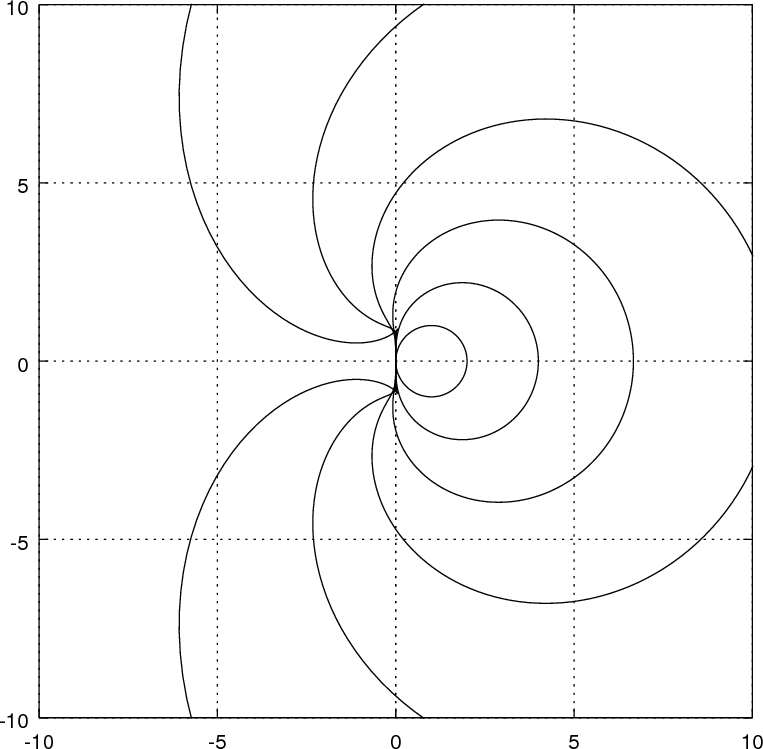
\includegraphics[width=.45\textwidth]{fig/stability-bdf.png}
  \hfill
  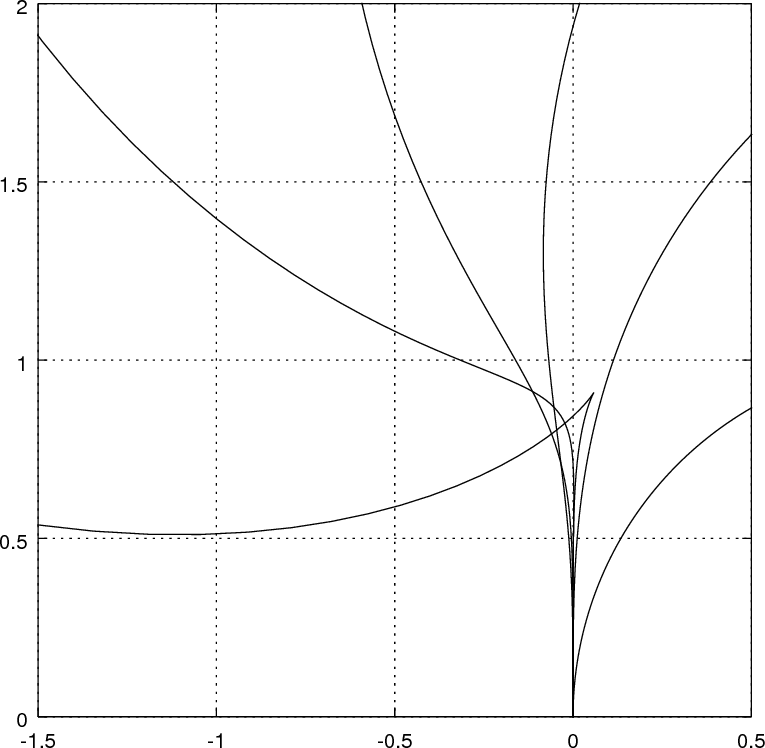
\includegraphics[width=.45\textwidth]{fig/stability-bdf-zoom.png}
  \caption{Boundaries of stability regions of BDF1 to BDF6. Unstable
    region right of the origin. Zoom on the right}
  \label{fig:bdf-stability}
\end{figure}
\begin{table}[tp]
  \centering
  \begin{tabular}{c|cccccc}
    $k$ & 1 & 2 & 3 & 4 & 5 & 6 \\\hline
    $\alpha$ & 90$^\circ$ & 90$^\circ$& 86.03$^\circ$
                    & 73.35$^\circ$& 51.84$^\circ$
                            & 17.84$^\circ$ \\
    $D$ & 0 & 0 & 0.083& 0.667& 2.327& 6.075
  \end{tabular}
  \caption{Values for A($\alpha$)- and stiff stability for BDF methods
    of order $k$.}
  \label{tab:bdf-stability}
\end{table}

%%%%%%%%%%%%%%%%%%%%%%%%%%%%%%%%%%%%%%%%%%%%%%%%%%%%%%%%%%%%%%%%%%%%%%
\section{Predictor-corrector schemes}

\begin{Definition*}{predictor-corrector}{Predictor-corrector methods}
  Assume a pair of time stepping schemes, one explicit, one implicit,
  \begin{align*}
    \hat y_{k} &= \hat \verfahren_p(y_{k-1}) \\
    y_k &= \verfahren_c(y_{k-1},y_{k}),
  \end{align*}
  we can use $\hat y_k$ as initial value for the Newton iteration for
  $y_k$. In an extreme case, we let
  \begin{gather*}
    y_k = \verfahren_c(y_{k-1},\hat y_{k}),
  \end{gather*}
  without any further iteration.
\end{Definition*}

\begin{remark}
  Predictor-corrector methods were developed strongly around
  Adams-Moulton and Adams-Bashforth methods, since the implicit ones
  have much smaller error constants. Given that these methods offer no
  considerable advantages compared to Runge-Kutta methods, but
  stability properties and implementation are weak points, We omit
  their discussion.

  A simple predictor for BDF methods can be obtained, since they are
  based on an interpolating polynomial. Thus, we simply extrapolate
  this polynomial to the next point in time.
\end{remark}

\begin{example}
  While the predictor-corrector idea sounds reasonable, we have to be
  careful with stiff problems, the original reason for using implicit
  methods. Take again our favorite IVP
  \begin{gather*}
    u' = \lambda u,
    \qquad u(0) = 1.
  \end{gather*}
  We apply the BDF(1) scheme, namely the implicit Euler method, with
  step size 1. According to its stability
  function~\eqref{eq:impl:stabil:impleuler}, we obtain
  \begin{gather*}
    y_1 = \frac1{1-\lambda}.
  \end{gather*}
  Hence, the interpolating polynomial is
  \begin{gather*}
    y(t) = (1-t) + \frac1{1-\lambda} t = 1 + \frac{\lambda}{1-\lambda}t.
  \end{gather*}
  For the mildly stiff problem $\lambda = -3$, we obtain
  \begin{gather*}
    y_1 = 0.25, \qquad y_2 = 0.0625,
    \qquad \hat y_2 = y(2) = -0.5.
  \end{gather*}
  Thus, the extrapolated value is already a much worse initial value
  for a Newton iteration than using the value from the previous time
  step.
  
  While this example was particularly chosen to exhibit such failure,
  it does show that extrapolation of stiff problems has its
  pitfalls. Here, we end up with a time step restriction which is
  comparable to the stability condition of the explicit method.
\end{example}


%%% Local Variables: 
%%% mode: latex
%%% TeX-master: "notes"
%%% End: 


\begin{remark}
  \index{step size!constant} The LMM was defined for constant step size
  $h$.  In principle it is possible to implement the method with a
  variable step size but we restrict ourselves to the constant case.
  Notes to the step size control can be found later on in this chapter.
\end{remark}

\begin{remark}
  One-step methods were always denoted by describing how to compute
  $y_1$ from $y_0$. Here, the notation becomes more complicated, but
  sometimes we consider only $y_s$ computed from $y_0,\dots,y_{s-1}$
  implying the same rules for $y_k$ computed from
  $y_{k-\lmms},\dots,y_{k-1}$.
\end{remark}
\begin{Definition}{lmm-errors}
    \index{Lh@$L_h$|textbf}
  We express the LMM with the linear \define{difference operator}
  \begin{gather}
    \label{eq:lmm:9}
    (L_hu)(t_k) = \sum_{r=0}^{\lmms}\Bigl(\alpha_{\lmms-r} u(t_{k-r}) - h
    \beta_{R-r} f\bigl(t_{k-r},u(t_{k-r})\bigr)\Bigr)
  \end{gather}
  and for a continuous function $u$ we define the \textbf{truncation
    error}\defindex{truncation error!LMM}
  \begin{gather}
    \label{eq:lmm:10}
    \tau_h(t_k) = \tfrac1hL_hu(t_k).
  \end{gather}
  The \textbf{local error} \defindex{LMM!local error}\defindex{local
    error!LMM} of a linear multistep method is defined by
  \begin{gather*}
    u(t_\lmms) - y_\lmms
  \end{gather*}
  where $u(t)$ denotes the exact solution of $u' = f(t,u), u(t_0)=u_0$
  and $y_s$ the numerical solution by using the exact initial values
 	$y_i = u(t_i)$ for $i = 0,1,...,s-1$.
\end{Definition}

%%% Local Variables:
%%% mode: latex
%%% TeX-master: "../notes"
%%% End:


\begin{lemma}
  Consider the differential equation
  \begin{gather*}
    y' = f(t,y) \qquad y(t_0) = y_0
  \end{gather*}
  where f is given continuously differentiable and $y(t)$ is the exact solution.
  For the local error we obtain

  \begin{gather}
    y(t_k)-y_k = \left( \alpha_0 \identity - h\beta_0 \frac{\partial f}{\partial y}(t_k,\eta) \right)^{-1} (L_h u)(t_k).
  \end{gather}

  Here $\eta$ is a value between $y(t_k)$ and $y_k$ if $f$ is a scalar
	function.
  If $f$ is multidimensional, the matrix 
	$\frac{\partial f}{\partial y}(t_k,\eta)$ is the Jacobi matrix, 
	which rows are evaluated at possible places between
	$y(t_k)$ and $y_k$.
\end{lemma}

\begin{proof}
  Considering the local error we can assume exact initial values 
  and therefore we can transform ~\ref{eq:lmm:4} to:
  \begin{gather*}
    \alpha_\lmms y_k + \sum\limits_{r=1}^\lmms \alpha_{\lmms-r} y(t_{k-r})
    = h \left( \beta_\lmms f_k + \sum\limits_{r=1}^\lmms \beta_{\lmms-r} f_{k-r} \right)
  \end{gather*}
  We transform further:
  \begin{multline*}
    \sum\limits_{r=0}^{\lmms} \left( \alpha_r y(t_{k-r})
      - h \beta_r f(t_{k-r},y(t_{k-r})) \right)
    \\
    - \alpha_0 y(t_k) + h \beta_0 f(t_k, y(t_k)) + \alpha_0 y_k
    - h \beta_0 f(t_k,y_k) = 0.
  \end{multline*}
	We now insert ~\ref{eq:lmm:9} which results in
  \begin{gather*}
    (L_h y)(t_k) = \alpha_0 \left( y(t_k) - y_k \right) - h \beta_0 \left( f(t_k,y(t_k)) - f(t_k,y_k) \right)
    \\
    \left( y(t_k) - y_k \right) \left( \alpha_0 \identity - h \beta_0 \frac{f(t_k,y(t_k)) - f(t_k,y_k)}{y(t_k) - y_k} \right)
  \end{gather*}
  By application of the mean value theorem and 
  subsequent transformation we obtain the statement of the theorem.
\end{proof}

      % \cite[Lemma 2.2, p. 369]{HairerNorsettWanner93}

\begin{Definition}{lmm-consistency}
  An LMM is consistent of order $p$, if for all sufficient regular
  functions $u$ and all relevant $k$ there holds
  \begin{gather}
    \label{eq:lmm:11}
    \tau_h(t_k) = \mathcal O(h^p),
  \end{gather}
  or equivalently, that the \putindex{local error} is $\mathcal O(h^{p+1})$.
\end{Definition}

%%% Local Variables:
%%% mode: latex
%%% TeX-master: "../notes"
%%% End:

\begin{Lemma}{lmm-bramble-hilbert}
  An LMM is consistent of order $p$ if and only if for all polynomials
  $\phi_q$ of degree $q \le p$ and $f(t,q(t)) = q'(t)$ there holds:
  \begin{gather}
    \label{eq:lmm:14}
    L_h \phi_q = 0.
  \end{gather}
\end{Lemma}

%%% Local Variables:
%%% mode: latex
%%% TeX-master: "../notes"
%%% End:


\begin{proof}
  We start with the Taylor expansion of a solution $u$ of the ODE and
  the corresponding right hand side $f$ for $t_k$, where we insert,
  unlike usual, $f=u'$:
  \begin{alignat*}2
    u(t) &= \sum_{i=0}^p \frac{u^{(i)}(t_k)}{i!}(t-t_k)^i +
    \frac{u^{(p+1)}(\xi)}{(p+1)!}(t-t_k)^{p+1} &=:& \phi(t) + r_u(t)
    \\
    f\bigl(t,u(t)\bigr) &= \sum_{i=1}^p \frac{u^{(i)}(t_k)}{(i-1)!}(t-t_k)^{i-1} +
    \frac{u^{(p+1)}(\xi)}{p!}(t-t_k)^{p} &=:& \phi'(t) + r_f(t),
  \end{alignat*}
  with the Taylor polynomial $\phi(t)$ of degree $p$ and remainder
  $r_u(t)$ and $r_f(t)$. Out of this we calculate:
  \begin{align*}
    L_h u(t_k) =& \sum_{r=0}^\lmms \alpha_{\lmms-r} \phi(t_{k-r}) - h
    \sum_{r=0}^\lmms \beta_{\lmms-r} \phi'(t_{k-r})
    \\
    &+ \sum_{r=0}^\lmms \alpha_{\lmms-r} r_u(t_{k-r}) - h
    \sum_{r=0}^\lmms \beta_{\lmms-r} r_f(t_{k-r}).
  \end{align*}
  Since $t_{k-r}-t_k = r h$, the first row equals a polynomial 
  $\psi(h)$ in $h$ of degree $p$. For the second row we insert the
	reminder estimate $r_u(t) = \mathcal O((t-t_k)^{p+1}) = h
  r_f(t)$ and get:
  \begin{gather}
    \label{eq:lmm:15}
    L_h u(t_k) = L_h \phi(t_k) + \mathcal O(h^{p+1}) = \psi(h) + \mathcal O(h^{p+1}).
  \end{gather}
  According to the definition of the truncation error, this term has to be of
	order $p+1$, such that the method is of order $p$. However it is $\psi$
  of degree $p$. This can only hold true if $L_h\phi=\psi\equiv
  0$. On the other hand $\tau_h(t_k)$ automatically is of order
  $p$. Since $u$ is the solution of an arbitrary right hand side, this
	condition has to be satisfied for all kind of Taylor polynomials $\phi$ 
	of degree $p$.
\end{proof}

\begin{Theorem}{lmm-consistency}
  \index{step size!constant}
  A LMM with constant step size is consistent of order
  $p$ if and only if
    \begin{gather}
      \label{eq:lmm:12}
      \begin{split}
      \sum_{r=0}^\lmms \alpha_{r} &= 0, \\
      \sum_{r=0}^\lmms \bigl(\alpha_{r}r^q - q \beta_{r}
      r^{q-1}\bigr) &= 0,
      \qquad q = 1,\dots,p        
      \end{split}
    \end{gather}
\end{Theorem}


\begin{proof}
  According to lemma~\ref{Lemma:lmm-bramble-hilbert} it is sufficient
  to show that ~\eqref{eq:lmm:12} is equivalent to $L_h \phi_q=0$ for
  polynomials of degree $q\le p$. Due to linearity of the method it
  however is sufficient to show this for a basis of the polynomial
  space of degree $p$.  For that we choose the monomial basis of the
  form
  \begin{gather*}
  \pi_q(t) =
  \left(\frac{t-t_{k-\lmms}}h\right)^q,\qquad q=0,\dots,p.
  \end{gather*}
  For those it holds: $\pi_q(t_{k-r}) = (\lmms-r)^q$. Now we see that
  the first condition is $L_h\pi_0 = 0$ (here is
  $\pi_0'\equiv0$) and the second condition is $L_h\pi_q = 0$.
\end{proof}

\begin{todo}
  Beispiel einer konsistenten LMM, die nicht konvergiert.
\end{todo}

\begin{remark}
  As shown in a homework problem, a consistent LMM is not necessary
  convergent. To understand this behavior and develop criteria for
  convergence we need to diverge into the theory of difference
  equations.
\end{remark}
%%%%%%%%%%%%%%%%%%%%%%%%%%%%%%%%%%%%%%%%%%%%%%%%%%%%%%%%%%%%%%%%%%%%%%
%%%%%%%%%%%%%%%%%%%%%%%%%%%%%%%%%%%%%%%%%%%%%%%%%%%%%%%%%%%%%%%%%%%%%%
\section{Properties of difference equations}
%%%%%%%%%%%%%%%%%%%%%%%%%%%%%%%%%%%%%%%%%%%%%%%%%%%%%%%%%%%%%%%%%%%%%%
%%%%%%%%%%%%%%%%%%%%%%%%%%%%%%%%%%%%%%%%%%%%%%%%%%%%%%%%%%%%%%%%%%%%%%

\begin{intro}
  The stability of LMM can be understood by employing the fairly old
  theory of difference equations. In order to keep the presentation
  simple in this section, we use a different notation for numbering
  indices in the equations. Nevertheless, the coefficients of the
  characteristic polynomial are the same as for LMM.
\end{intro}

\begin{Definition}{difference-equation}
  An equation of the form
  \begin{gather}
    \label{eq:lmm:3}
    \sum_{r=0}^\lmms \alpha_{r} y_{n+r} = 0
  \end{gather}
  is called a homogeneous \define{difference equation}. A sequence
  $\{y_n\}_{n=0,\dots,\infty}$ is solution of the difference equation,
  if the equation holds true for all $n\ge \lmms$. The values
  $y_n$ may be from any of the spaces $\R$, $\C$, $\R^d$ or $\C^d$.

  The \define{generating polynomial} of this difference equation
  is
  \begin{gather}
    \label{eq:lmm:2}
    \chi(x) = \sum_{r=0}^\lmms \alpha_{r} x^{r}.
  \end{gather}

\end{Definition}

%%% Local Variables:
%%% mode: latex
%%% TeX-master: "../notes"
%%% End:


\begin{Lemma}{lmm:1}
  The solutions of the equation~\eqref{eq:lmm:3} with $y_n\in \R$ or
  $y_n\in \C$ form a vector space of dimension $\lmms$. 
\end{Lemma}

\begin{proof}
  Since the equation~\eqref{eq:lmm:3} is linear and homogeneous, it is
  obvious that if two sequences of solutions $\{y^{(1)}\}$ and
  $\{y^{(2)}\}$ satisfy the equation, sums of multiples of them
  satisfy it too.

  As soon as the initial values $y_0$ to $y_{\lmms-1}$ are chosen, all
  other sequence members are uniquely defined.  Moreover it holds
  \begin{gather*}
    y_0=y_1=\dots=y_{\lmms-1}=0
    \quad\Longrightarrow\quad
    y_n = 0, \;n \ge 0.
  \end{gather*}
  Therefore it is sufficient to consider the first $\lmms$ values.  If
  they are linear independent, then the overall sequences are and vice
  versa. Thus, the initial values form a $\lmms$
  dimensional vector space.
\end{proof}

\begin{Lemma}{difference-equation-solutions}
  For each root $\xi$ of the generating polynomial $\chi(x)$ the
  sequence $y_n = \xi^n$ is a solution of the difference
  equation~\eqref{eq:lmm:3}.
\end{Lemma}


%%% Local Variables: 
%%% mode: latex
%%% TeX-master: "../notes"
%%% End: 


\begin{proof}
  Inserting the solution $y_n = \xi^n$ into the difference equation
  results in
  \begin{gather*}
    \sum_{r=0}^\lmms \alpha_{r} \xi^{n+r} = \xi^{n}
    \sum_{r=0}^\lmms \alpha_{r} \xi^{r}
    = \xi^{n} \chi(\xi) = 0.
  \end{gather*}
\end{proof}

\begin{Theorem}{difference-equation-basis}
  Let $\{\xi_i\}_{i=1,\dots,\iota}$ be the roots of the
  generating polynomial $\chi$ with multiplicity $\nu_i$. Then,
  the sequences of the form
  \begin{gather}
    \label{eq:lmm:6}
%    y^{(i,k)}_n = p_k(n)\xi_i^n
    y^{(i,k)}_n = n^{k-1}\xi_i^n
    \quad i=1,\dots,\iota; \quad k = 1,\dots,\nu_i
  \end{gather}
%  mit den Polynomen
%  \begin{gather*}
%    p_0(n) = 1 \quad p_k(n) = \prod_{\kappa=0}^{k-1} (n-\kappa)
%  \end{gather*}
  form a basis of the solution space of the difference
  equation~\eqref{eq:lmm:3}.
\end{Theorem}


%%% Local Variables: 
%%% mode: latex
%%% TeX-master: "../notes"
%%% End: 


\begin{proof}
  First we observe that the sum of the multiplicities of the roots
  results in the degree of the polynomial:
  \begin{gather*}
    \lmms = \sum_{i=1}^\iota \nu_i.
  \end{gather*}
  Moreover we know because of Lemma~\ref{Lemma:lmm:1}, that $\lmms$ is
  the dimension of the solution space. We show that the sequences
  $\{y^{(i,k)}_n\}$ are linear independent. This is clear for
  sequences of different index $i$. It is also clear for different roots,
  because for $n\to\infty$ the exponential function nullifies the
  influence of the polynomials.
  
  It remains to show that the sequences $\{y^{(i,k)}_n\}$ in fact are
  solutions of the difference equations.  For $k=0$ we have proven
  this already in lemma~\ref{Lemma:difference-equation-solutions}.  We proof the fact here for
  $k=2$ and for a double zero $\xi_i$; the principle for higher order
  roots should be clear then.  Equation~\eqref{eq:lmm:3} applied to
  the sequence $\{n \xi_i^n\}$ results in
  \begin{align*}
    \sum_{r=0}^{\lmms} \alpha_r (n+r) \xi_i^{n+r}
    &= n \xi_i^n \sum_{r=0}^{\lmms} \alpha_r \xi_i^{r}
    + \xi_i^{n+1} \sum_{r=1}^{\lmms} \alpha_r r \xi_i^{r-1}
    \\
    &= n \xi_i^n \rho(\xi_i) + \xi_i^{n+1} \rho'(\xi_i) = 0.
  \end{align*}
  Here the term with $\alpha_0$ vanishes, because it is multiplied
  with $r=0$. $\rho(\xi_i) = \rho'(\xi_i) = 0$ because $\xi_i$ is a
  multiple root.
\end{proof}

\begin{Corollary*}{root-test}{Root test}
  All solutions $\{y_n\}$ of the difference equation~\eqref{eq:lmm:3}
  are bounded for $n\to\infty$ if and only if it holds:
  \begin{itemize}
  \item all roots of the generating polynomial $\chi(x)$
    lie in the closed unit circle $\bigl\{z\in \C \big|\; |z|\le
    1\bigr\}$ and
  \item all roots on the boundary of the unit circle are simple.
  \end{itemize}
\end{Corollary*}

%%% Local Variables: 
%%% mode: latex
%%% TeX-master: "../notes"
%%% End: 


\begin{proof}
  According to theorem~\ref{Theorem:difference-equation-basis} we can write all solutions
  as linear combinations of the sequences $y^{(i,k)}$ in
  equation~\eqref{eq:lmm:6}. Therefore,
  \begin{enumerate}
  \item all solutions to $|\xi_i|<1$ for $n\to\infty$ converge to zero
  \item all solutions to $|\xi_i|>1$ for $n\to\infty$ divergence to infinity
  \item all solutions to $|\xi_i|=1$ for $n\to\infty$ stay bounded 
	if and only if $\xi_i$ is simple.
  \end{enumerate}
  This proves the statement of the theorem.
\end{proof}

%%%%%%%%%%%%%%%%%%%%%%%%%%%%%%%%%%%%%%%%%%%%%%%%%%%%%%%%%%%%%%%%%%%%%%
%%%%%%%%%%%%%%%%%%%%%%%%%%%%%%%%%%%%%%%%%%%%%%%%%%%%%%%%%%%%%%%%%%%%%%
\section{Stability and convergence}
%%%%%%%%%%%%%%%%%%%%%%%%%%%%%%%%%%%%%%%%%%%%%%%%%%%%%%%%%%%%%%%%%%%%%%
%%%%%%%%%%%%%%%%%%%%%%%%%%%%%%%%%%%%%%%%%%%%%%%%%%%%%%%%%%%%%%%%%%%%%%

\begin{remark}
  In contrast to one-step methods the convergence of multistep methods
  follows not directly from the consistency of the method, if the
  right hand side of the differential equation satisfies the Lipschitz
  condition~\eqref{eq:IVP:1}.  Analog to the A-stability we will
  discuss this by means of a simple model problem and we will deduce
  stability conditions.
\end{remark}

\begin{remark}
  In the following we investigate the solution to a fixed point in time
  $t$ with a shrinking step size $h$. Therefore we choose $n$
  steps of step size $h = t/n$ and let $n$ go towards infinity.
\end{remark}

\begin{Theorem}{lmm-stability}
  A LMM is stable if and only if all roots of the first
  generating polynomial $\rho(x)$ of equation~\eqref{eq:lmm:5} lie
  in the unit circle of the complex plane and all roots on the
  boundary of the unit circle are simple.
\end{Theorem}


%%% Local Variables: 
%%% mode: latex
%%% TeX-master: "../notes"
%%% End: 

\begin{Theorem}{lmm-stability}
  A LMM is stable if and only if all roots of the first
  generating polynomial $\rho(x)$ of equation~\eqref{eq:lmm:5} lie
  in the unit circle of the complex plane and all roots on the
  boundary of the unit circle are simple.
\end{Theorem}


%%% Local Variables: 
%%% mode: latex
%%% TeX-master: "../notes"
%%% End: 


\begin{proof}
  The application of the LMM to the equation~\eqref{eq:lmm:1} results
  in the difference equation
  \begin{gather*}
    \sum_{r=0}^{\lmms} \alpha_{\lmms-r} y_{n-r} = 0.
  \end{gather*}
  Now we have to proof that the solutions for fixed $t = h n$ stay
  bounded if $h\to 0$. But we also see that the upper equation does
  not contain $h$. Therefore we have to examine, if the solutions
  $y_n$ stay bounded for $n\to \infty$.  By resorting the summation we
  obtain a difference equation of the form~\eqref{eq:lmm:3}. Due to
  corollary~\ref{Corollary:root-test} it follows the statement of the theorem.
\end{proof}

\begin{Corollary}{adams-stability}
  Adams-Bashforth and Adams-Moulton methods are stable.
\end{Corollary}

\begin{proof}
  For all of these methods the first generating polynomial is $\rho(x)
  = x^\lmms-x^{\lmms-1}$. It has the simple root $\xi_1 = 1$ and the
  $\lmms-1$-fold root 0.
\end{proof}

\begin{Theorem}{BDF-stability}
  The BDF methods are stable for $\lmms \le 6$ and not
  stable for $\lmms \ge 7$.
\end{Theorem}

\begin{Theorem}{lmm-convergence}
  If a linear multi-step method is stable and consistent of order $p$,
  then it is convergent of order $p$.
\end{Theorem}

%%% Local Variables: 
%%% mode: latex
%%% TeX-master: "../notes"
%%% End: 

\begin{Lemma}{lmm-one-step}
  Every multistep method can be recast as a one-step method
  \begin{gather}
    \label{eq:lmm-one-step:1}
    Y_{k} = (A \otimes \identity) Y_{k-1} + h \verfahren_h(t_{k-1}, Y_{k-1})
  \end{gather}
  where with $\alpha_r' = \alpha_r/\alpha_s$
  \begin{gather}
    \label{eq:lmm-one-step:2}
    Y_k =
    \begin{pmatrix}
      y_k \\ \vdots \\ y_{k-s+1}
    \end{pmatrix},
    \quad
    A =
    \begin{pmatrix}
      -\alpha_{\lmms-1}' & -\alpha_{\lmms-2}' & \cdots & -\alpha_{0}'\\
      1 & 0 & \cdots & 0 \\
      & \ddots & \cdots & 0 \\
      & & 1 & 0
    \end{pmatrix},
  \end{gather}
  and $\verfahren_h(t_k, Y_k) = (e_1 \otimes \identity) \psi_h(t_{k-1}, Y_{k-1})$ with
  $\beta_r' = \beta_r/\alpha_s$ and $\psi_h$ defined implicitly by
  \begin{multline}
    \label{eq:lmm-one-step:3}
    \psi_h(t_{k-1}, Y_{k-1})
    =\sum_{r=1}^{\lmms} \beta_{\lmms-r} f(t_{k-r},y_{k-r})
    \\
    + \beta_s' f\left(t_k, h\psi_h(t_{k-1}, Y_{k-1}) -
      \sum_{r=1}^{\lmms} \alpha_{\lmms-r}' y_{k-r}\right).
  \end{multline}
\end{Lemma}

%%% Local Variables: 
%%% mode: latex
%%% TeX-master: "../notes"
%%% End: 


\begin{proof}
  From the general form of LMM we
  obtain
  \begin{gather*}
    \frac1{\alpha_s} \sum_{r=0}^\lmms \alpha_{\lmms-r} y_{k-r}
    = \frac{h}{\alpha_s} \sum_{r=0}^{\lmms-1} \beta_{\lmms-r} f_{k-r}
    + \beta_s f_k.
  \end{gather*}
  We rewrite this to
  \begin{gather*}
    y_k = -\sum_{r=1}^{\lmms} \alpha'_{\lmms-r} y_{k-r} +
    h\psi_h(t_{k-1}, Y_{k-1}),
  \end{gather*}
  where we implicitly enter this formula as value for $y_k$ in the
  computation of $f_k$. It remains to realize that this is the first
  set of $d$ equations in~\eqref{eq:lmm-one-step:1}, and that the
  remaining ones are just shifting $y_i$ to $y_{i+1}$.
\end{proof}

\begin{Lemma}{lmm-one-consistency}
  Let $u(t)$ be the exact solution of the IVP. For $k=s,\ldots$, we
  define the vector $\widehat Y_{k}$ as the solution of a single step
  \begin{gather*}
    \widehat Y_{k} = (A\otimes I) U_{k-1} + h \verfahren_h(t_{k-1} U_{k-1}),
  \end{gather*}
  with correct initial values $U_{k-1} =
  (u_{k-1},u_{k-2},\dots,u_{k-\lmms})^T$.
  
  If the multistep method is consistent of order $p$, and $f$ is
  sufficiently smooth, then there exist constants $h_0>0$  and $M$
  such that for $h\le h_0$ there holds
  \begin{gather}
    \label{eq:lmm-one-consistency:1}
    \norm{Y_k-\widehat Y_h} \le M h^{p+1}.
  \end{gather}
\end{Lemma}

%%% Local Variables: 
%%% mode: latex
%%% TeX-master: "../notes"
%%% End: 


\begin{proof}
  The first component of $Y_k - \widehat Y_k$ is the local error of
  step $k$, which is of order $h^{p+1}$ by the assumption. The other
  components vanish by the definition of the method.
\end{proof}

\begin{Lemma}{lmm-one-stability}
  Assume that an LMM is stable. Then, there exists a vector norm on
  $\C^{\lmms d}$ such that the operator norm of the matrix $A$
  satisfies
  \begin{gather}
    \label{eq:lmm-one-stability:1}
    \norm{A\otimes \identity} \le 1.
  \end{gather}
\end{Lemma}

%%% Local Variables: 
%%% mode: latex
%%% TeX-master: "../notes"
%%% End: 


\begin{proof}
  We notice that $\widehat\rho(x) = \sum \alpha'_{s-r} x^r$ is the
  characteristic polynomial of the matrix $A$ and thus its eigenvalues
  are the roots of $\widehat\rho(x)$, which has the same roots as the
  generating polynomial $\rho(x)$. By the root test, we know that
  simple roots, which correspond to irreducible blocks of dimension
  one have maximal modulus one. Furthermore, every Jordan block of
  dimension greater than one corresponds to a multiple root, which by
  assumption has modulus strictly less than one. It is easy to see
  that such a block admits a modified canonical form
  \begin{gather*}
    J_i =
    \begin{pmatrix}
      \lambda_i & 1- \abs{\lambda_i}\\
        & \lambda_i &\ddots\\
          &&\ddots & 1- \abs{\lambda_i}\\
            &&&\lambda_i
    \end{pmatrix}.
  \end{gather*}
  Thus, the canonical form $J = T^{-1}AT$ has norm $\norm{J}_{\infty}
  \le 1$. If we define the norm
  \begin{gather*}
    \norm{x} = \norm{(T^{-1}\otimes \identity)x}_\infty,
  \end{gather*}
  we obtain the result by
  \begin{multline*}
    \norm{(A\otimes \identity)x}
    = \norm{(T^{-1}\otimes \identity)(A\otimes \identity)x}_\infty
    = \norm{(J\otimes \identity)(T^{-1}\otimes \identity)x}_\infty
    \\
    \le \norm{(T^{-1}\otimes \identity)x}_\infty
    = \norm{x}.
  \end{multline*}
\end{proof}

\begin{Theorem}{lmm-convergence}
  If a linear multi-step method is stable and consistent of order $p$,
  then it is convergent of order $p$.
\end{Theorem}

%%% Local Variables: 
%%% mode: latex
%%% TeX-master: "../notes"
%%% End: 


\begin{proof}
  We reduce the proof to convergence of a one-step method with
  \begin{gather}
    \label{eq:lmm:18}
    Y_k = G(Y_{k-1}) =  (A\otimes \identity) Y_{k-1} + h \verfahren_h(t_{k-1}, Y_{k-1}).
  \end{gather}
  Let $Y_{k-1}$ and $Z_{k-1}$ be two initial values for the interval $I_k$.
  By the previous lemma, we have in the norm defined there, for
  sufficiently small $h$, and assuming a Lipschitz constant $L_h$ for
  $\verfahren_h$ :
  \begin{gather}
    \label{eq:lmm:19}
    \norm{G(Y_{k-1})-G(Z_{k-1})} \le (1+h L_h) \norm{Y_{k-1}-Z_{k-1}}.
  \end{gather}
  Thus, the local error $\eta_k = U_k - \widehat Y_k$ at step $k$, which by
  Lemma~\ref{Lemma:lmm-one-consistency} is bounded by $M h^{p+1}$, accumulates
  until step $n$ at most to $h^{p+1}(1_h L_h)^{n-k}$.

  We have:
  \begin{align*}
    \norm{U_1 - Y_1} &\le (1+h L_h)\norm{U_0-y_0} + M h^{p+1} \\
    \norm{U_2 - Y_2} &\le (1+h L_h)^2\norm{U_0-y_0} +  M h^{p+1} \bigl(1+ (1+h L_h)\bigr)\\
    \norm{U_3 - Y_3} &\le (1+h L_h)^3\norm{U_0-y_0} +  M h^{p+1} \Bigl(\bigl(1+ (1+h L_h)+ (1+h L_h)^2\bigr)\Bigr)\\
    \norm{U_n-Y_n} &\le e^{n h L_h}\norm{U_0-Y_0} +
    \frac{M h^p}{L_h}\bigl(e^{n h L_h} - 1\bigr).
  \end{align*}
\end{proof}

\subsection{Starting procedures}

\begin{intro}
In contrast to one-step methods, where the numerical solution is obtained 
solely from the differential equation and the initial value, multistep 
methods require more than one start value. An LMM with $s$ steps requires $s$ 
known start values $y_{k-s}, \dots, y_{k-1}$. Mostly, they are not provided 
by the IVP itself. Thus, general LMM decompose into two parts: 
\begin{itemize}
\item a \emph{starting phase} where the start values are computed in a 
suitable way and
\item a \emph{run phase} where the LMM is executed. 
\end{itemize}
It is crucial that the method of the starting phase provides a suitable order 
corresponding to the LMM of the run phase, recall Definition 
\ref{Definition:lmm-convergence}. Moreover, it should have analog properties to 
the LMM, like explicit/implicit or applicability to stiff problems. 
% We now consider different starting procedures for an implicit LMM with 
% convergence order $p$. According to Definition \ref{Definition:lmm-convergence} 
% the starting values are required to have the same convergence order. 
Possible choices for the starting phase include multistep methods with variable 
order and one-step methods.  
\end{intro}

\begin{example}[Self starter]
A 2-step BDF method requires $y_0$ and $y_1$ to be known. $y_0$ is given by the 
initial value while $y_1$ is unknown so far. To guarantee that the method has 
order 2, $y_1$ needs to be locally of order 2 at least
\begin{align}\label{eq:lmm_1BDFstarter}
|u(t_1)-y_1| \leq c_0 h^2.
\end{align}
This is ensured, for example, by one step of the 1-step BDF method.

However, starting an LMM with $s>2$ steps by a first-order method and then 
successively increasing the order until $s$ is reached does not provide the 
desired global order. That is due to the fact that the first step limits  
the overall convergence order to 2, compare \eqref{eq:lmm_1BDFstarter}. 
Nevertheless, self starters are often used in practice. 
\end{example}
% In this case local 
% error estimates are used to bound the errors of the starting values and all 
% approximations of the run phase by reducing the step sizes, 
% %. Moreover, also in 
% %the run phase the step sizes are controlled using local error estimates, 
% see the  
% discussion on step size control in Section \ref{section:step_size_control}. 


\begin{example}[Runge-Kutta starter]
\label{Example:RKstarter}
One can use Runge-Kutta methods to start LMM. Since only a fixed
number of starting steps are performed, the local order of the
Runge-Kutta approximation is crucial.  For an implicit LMM with
convergence order $p$ and stepsize $h$ one could use an RK method with
consistency order $p-1$ with the same stepsize $h$.

Consider a 3-step BDF method. Thus, beside $y_0$, we need start values 
$y_1, y_2$ with errors less than $c_0 h^3$. They can be computed by RK methods 
of consistency order $2$, for example by two steps of the 1-stage Gau\ss \ 
collocation method with step size $h$ since it has consistency order $2s=2$, 
see theorem \ref{Theorem:gauss-consistency}.
\end{example}




\begin{example}[Continuous Runge-Kutta starter]
  Another option is to use continuous Runge-Kutta methods and to
  evaluate the continuous approximation to obtain the required
  starting values.

  In constrast to Example \ref{Example:RKstarter} one could also use
  the continuous polynomial approximation of Gau\ss \ collocation to
  start a 3-step BDF method. One step with step size $2h$ of a 2-stage
  Gau\ss \ collocation method would give a polynomial of degree $2$
  which is then evaluated in $t_1=t_0+h$ and $t_2=t_1+h$ to obtain
  $y_1, y_2$. According to Theorem
  \ref{Theorem:collocation-continuous} $y_1, y_2$ have the appropriate
  order.
\end{example}

\begin{remark}
  In practice not the order of a procedure is crucial but rather the
  fact that the errors of all approximations (the start values and all
  approximations of the run phase) are bounded by the user-given
  tolerance, compare Section \ref{section:step_size_control}. Thus,
  the step sizes of all steps are controlled using local error
  estimates. Hence, self starting procedures usually start with very
  small step sizes and increase them successively. Due to their higher
  orders RK starters usually are allowed to use moderate step sizes in
  the beginning. Generally, LMM are applied with variable step sizes
  and orders in practice (see e.g. Exercise 7.2).
\end{remark}



%%%%%%%%%%%%%%%%%%%%%%%%%%%%%%%%%%%%%%%%%%%%%%%%%%%%%%%%%%%%%%%%%%%%%%
%%%%%%%%%%%%%%%%%%%%%%%%%%%%%%%%%%%%%%%%%%%%%%%%%%%%%%%%%%%%%%%%%%%%%%
\section{LMM and stiff problems}
%%%%%%%%%%%%%%%%%%%%%%%%%%%%%%%%%%%%%%%%%%%%%%%%%%%%%%%%%%%%%%%%%%%%%%
%%%%%%%%%%%%%%%%%%%%%%%%%%%%%%%%%%%%%%%%%%%%%%%%%%%%%%%%%%%%%%%%%%%%%%

\begin{Definition*}{lmm-stability-region}{A-stability of LMM}
  \index{stability region!of a LMM}
  The linear model difference equation
  \begin{gather}
    \label{eq:lmm:7}
    \sum_{r=0}^{\lmms} \bigl(\alpha_{\lmms-r} - z \beta_{\lmms-r}) y_{n-r} = 0.
  \end{gather}
  is obtained by applying an LMM to the model equation
  $u' = \lambda u$ and inserting $z=h\lambda$.

  The \define{stability region} of an LMM is the set of points $z\in \C$,
  for which all solution sequences $\{y_n\}$ of the equation~\eqref{eq:lmm:7}
  stay bounded for $n\to\infty$. An LMM is called \define{A-stable}, if the 
  stability region contains the left half-plane of $\C$.
\end{Definition*}


\begin{Definition}{lmm-stability-polynomial}
  The stability polynomial of an LMM is obtained by inserting
  $y_n = x^n$ into the linear model difference equation to obtain
  \begin{gather}
    \label{eq:lmm:8}
    r_z(x) = \sum_{r=0}^{\lmms} \bigl(\alpha_{\lmms-r} - z \beta_{\lmms-r})
    x^{\lmms-r}.
  \end{gather}
\end{Definition}

\begin{remark}
  Instead of the simple amplification function $r(z)$ of the one-step
  methods, we get here a function of two variables.  The point $z$ for
  which we want to show stability and the artificial variable $x$ from
  the analysis of the method.
\end{remark}

\begin{Lemma}{lmm-stability}
  Let $\{\xi_1(z),\dots,\xi_\lmms(z)\}$ be the set of roots of the
  stability polynomial $r_z(x)$ as functions of $z$.
  A point $z\in \C$ is in the stability region of a LMM, if these
  roots satisfy the root test in corollary~\ref{Corollary:root-test}.
\end{Lemma}

\begin{proof}
  The proof is analog to theorem~\ref{Theorem:lmm-stability}.
\end{proof}

\begin{Theorem*}{dahlquist2}{2nd Dahlquist barrier}
  \defindex{Dahlquist barrier (second)} There is no A-stable LMM of
  order $p>2$. Among the A-stable LMM of order 2, the trapezoidal rule
  (Crank-Nicolson) has the smallest error constant.
\end{Theorem*}

\subsection{Relaxed A-stability}

\begin{intro}
  Motivated by the fact that there are no higher order A-stable LMM
  and by highly dissipative problems, people have introduced relaxed
  concepts of A-stability.
\end{intro}

\begin{Definition}{aa-stability}
  \defindex{A($\alpha$)-stable}
  A set is called \textbf{A($\alpha$)-stable}, if its stability region
  contains the sector
  \begin{gather*}
    \bigg\{z\in \C\;\bigg|\; \Re z < 0 \;\wedge\; \left|\frac{\Im
        z}{\Re z}\right| \le \tan \alpha\biggr\}.
  \end{gather*}
  It is called \textbf{A(0)-stable}, if the negative real axis is contained in
  the stability region.

  It is called \define{stiffly stable}, if it contains the set
  $\{\Re(z)< -D\}$.
\end{Definition}

%%% Local Variables:
%%% mode: latex
%%% TeX-master: "../notes"
%%% End:


\begin{remark}
  The introduction of the A(0)-stability is motivated by linear
  systems of the form $u'=-Au$ with symmetric, positive definite
  matrix $A$. In fact one requires there only stability on the real
  axis because all eigenvalues are real. Thus, any positive angle
  $\alpha$ is sufficient.
  
  Similarly A($\alpha$)-stable LMM are suitable for linear problems in
  which high frequently vibration ($\Im\lambda$ large) decay fast
  ($-\Re\lambda$ large).

  In all cases one observes corresponding properties of the Jacobian
  matrix $\partial_u f$ for the application of nonlinear problems.
\end{remark}

\begin{example}
  The stability regions of the stable BDF methods are in
  Figure~\ref{fig:bdf-stability}. The corresponding values for
  A($\alpha$)-stability and stiff stability are in Table  
\ref{tab:bdf-stability}.
\end{example}
\begin{figure}[tp]
  \centering
  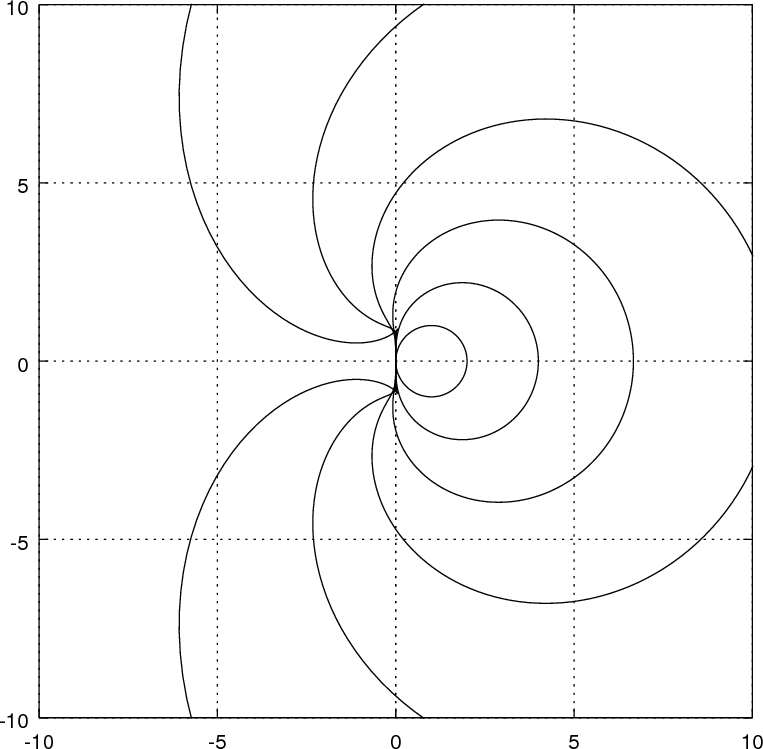
\includegraphics[width=.45\textwidth]{fig/stability-bdf.png}
  \hfill
  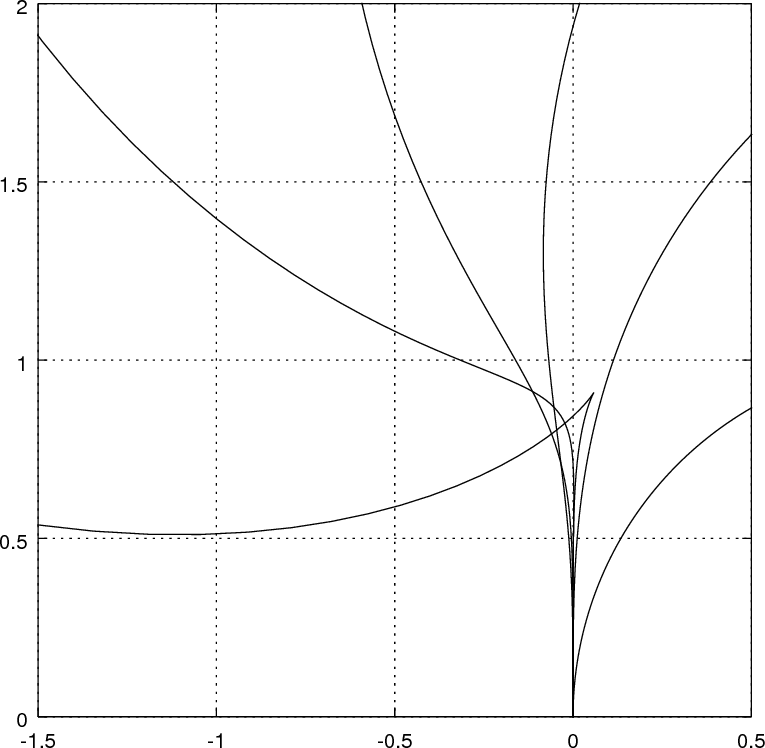
\includegraphics[width=.45\textwidth]{fig/stability-bdf-zoom.png}
  \caption{Boundaries of stability regions of BDF1 to BDF6. Unstable
    region right of the origin. Zoom on the right}
  \label{fig:bdf-stability}
\end{figure}
\begin{table}[tp]
  \centering
  \begin{tabular}{c|cccccc}
    $k$ & 1 & 2 & 3 & 4 & 5 & 6 \\\hline
    $\alpha$ & 90$^\circ$ & 90$^\circ$& 86.03$^\circ$
                    & 73.35$^\circ$& 51.84$^\circ$
                            & 17.84$^\circ$ \\
    $D$ & 0 & 0 & 0.083& 0.667& 2.327& 6.075
  \end{tabular}
  \caption{Values for A($\alpha$)- and stiff stability for BDF methods
    of order $k$.}
  \label{tab:bdf-stability}
\end{table}

%%%%%%%%%%%%%%%%%%%%%%%%%%%%%%%%%%%%%%%%%%%%%%%%%%%%%%%%%%%%%%%%%%%%%%
\section{Predictor-corrector schemes}

\begin{Definition*}{predictor-corrector}{Predictor-corrector methods}
  Assume a pair of time stepping schemes, one explicit, one implicit,
  \begin{align*}
    \hat y_{k} &= \hat \verfahren_p(y_{k-1}) \\
    y_k &= \verfahren_c(y_{k-1},y_{k}),
  \end{align*}
  we can use $\hat y_k$ as initial value for the Newton iteration for
  $y_k$. In an extreme case, we let
  \begin{gather*}
    y_k = \verfahren_c(y_{k-1},\hat y_{k}),
  \end{gather*}
  without any further iteration.
\end{Definition*}

\begin{remark}
  Predictor-corrector methods were developed strongly around
  Adams-Moulton and Adams-Bashforth methods, since the implicit ones
  have much smaller error constants. Given that these methods offer no
  considerable advantages compared to Runge-Kutta methods, but
  stability properties and implementation are weak points, We omit
  their discussion.

  A simple predictor for BDF methods can be obtained, since they are
  based on an interpolating polynomial. Thus, we simply extrapolate
  this polynomial to the next point in time.
\end{remark}

\begin{example}
  While the predictor-corrector idea sounds reasonable, we have to be
  careful with stiff problems, the original reason for using implicit
  methods. Take again our favorite IVP
  \begin{gather*}
    u' = \lambda u,
    \qquad u(0) = 1.
  \end{gather*}
  We apply the BDF(1) scheme, namely the implicit Euler method, with
  step size 1. According to its stability
  function~\eqref{eq:impl:stabil:impleuler}, we obtain
  \begin{gather*}
    y_1 = \frac1{1-\lambda}.
  \end{gather*}
  Hence, the interpolating polynomial is
  \begin{gather*}
    y(t) = (1-t) + \frac1{1-\lambda} t = 1 + \frac{\lambda}{1-\lambda}t.
  \end{gather*}
  For the mildly stiff problem $\lambda = -3$, we obtain
  \begin{gather*}
    y_1 = 0.25, \qquad y_2 = 0.0625,
    \qquad \hat y_2 = y(2) = -0.5.
  \end{gather*}
  Thus, the extrapolated value is already a much worse initial value
  for a Newton iteration than using the value from the previous time
  step.
  
  While this example was particularly chosen to exhibit such failure,
  it does show that extrapolation of stiff problems has its
  pitfalls. Here, we end up with a time step restriction which is
  comparable to the stability condition of the explicit method.
\end{example}


%%% Local Variables: 
%%% mode: latex
%%% TeX-master: "notes"
%%% End: 
}
\frame{\begin{Definition}{lmm-errors}
    \index{Lh@$L_h$|textbf}
  We express the LMM with the linear \define{difference operator}
  \begin{gather}
    \label{eq:lmm:9}
    (L_hu)(t_k) = \sum_{r=0}^{\lmms}\Bigl(\alpha_{\lmms-r} u(t_{k-r}) - h
    \beta_{R-r} f\bigl(t_{k-r},u(t_{k-r})\bigr)\Bigr)
  \end{gather}
  and for a continuous function $u$ we define the \textbf{truncation
    error}\defindex{truncation error!LMM}
  \begin{gather}
    \label{eq:lmm:10}
    \tau_h(t_k) = \tfrac1hL_hu(t_k).
  \end{gather}
  The \textbf{local error} \defindex{LMM!local error}\defindex{local
    error!LMM} of a linear multistep method is defined by
  \begin{gather*}
    u(t_\lmms) - y_\lmms
  \end{gather*}
  where $u(t)$ denotes the exact solution of $u' = f(t,u), u(t_0)=u_0$
  and $y_s$ the numerical solution by using the exact initial values
 	$y_i = u(t_i)$ for $i = 0,1,...,s-1$.
\end{Definition}

%%% Local Variables:
%%% mode: latex
%%% TeX-master: "../notes"
%%% End:
}
\frame{\begin{Definition}{lmm-consistency}
  An LMM is consistent of order $p$, if for all sufficient regular
  functions $u$ and all relevant $k$ there holds
  \begin{gather}
    \label{eq:lmm:11}
    \tau_h(t_k) = \mathcal O(h^p),
  \end{gather}
  or equivalently, that the \putindex{local error} is $\mathcal O(h^{p+1})$.
\end{Definition}

%%% Local Variables:
%%% mode: latex
%%% TeX-master: "../notes"
%%% End:

\begin{Lemma}{lmm-bramble-hilbert}
  An LMM is consistent of order $p$ if and only if for all polynomials
  $\phi_q$ of degree $q \le p$ and $f(t,q(t)) = q'(t)$ there holds:
  \begin{gather}
    \label{eq:lmm:14}
    L_h \phi_q = 0.
  \end{gather}
\end{Lemma}

%%% Local Variables:
%%% mode: latex
%%% TeX-master: "../notes"
%%% End:
}
\frame{\begin{Definition}{difference-equation}
  An equation of the form
  \begin{gather}
    \label{eq:lmm:3}
    \sum_{r=0}^\lmms \alpha_{r} y_{n+r} = 0
  \end{gather}
  is called a homogeneous \define{difference equation}. A sequence
  $\{y_n\}_{n=0,\dots,\infty}$ is solution of the difference equation,
  if the equation holds true for all $n\ge \lmms$. The values
  $y_n$ may be from any of the spaces $\R$, $\C$, $\R^d$ or $\C^d$.

  The \define{generating polynomial} of this difference equation
  is
  \begin{gather}
    \label{eq:lmm:2}
    \chi(x) = \sum_{r=0}^\lmms \alpha_{r} x^{r}.
  \end{gather}

\end{Definition}

%%% Local Variables:
%%% mode: latex
%%% TeX-master: "../notes"
%%% End:
}
\frame{\begin{Lemma}{difference-equation-solutions}
  For each root $\xi$ of the generating polynomial $\chi(x)$ the
  sequence $y_n = \xi^n$ is a solution of the difference
  equation~\eqref{eq:lmm:3}.
\end{Lemma}


%%% Local Variables: 
%%% mode: latex
%%% TeX-master: "../notes"
%%% End: 

\begin{Theorem}{difference-equation-basis}
  Let $\{\xi_i\}_{i=1,\dots,\iota}$ be the roots of the
  generating polynomial $\chi$ with multiplicity $\nu_i$. Then,
  the sequences of the form
  \begin{gather}
    \label{eq:lmm:6}
%    y^{(i,k)}_n = p_k(n)\xi_i^n
    y^{(i,k)}_n = n^{k-1}\xi_i^n
    \quad i=1,\dots,\iota; \quad k = 1,\dots,\nu_i
  \end{gather}
%  mit den Polynomen
%  \begin{gather*}
%    p_0(n) = 1 \quad p_k(n) = \prod_{\kappa=0}^{k-1} (n-\kappa)
%  \end{gather*}
  form a basis of the solution space of the difference
  equation~\eqref{eq:lmm:3}.
\end{Theorem}


%%% Local Variables: 
%%% mode: latex
%%% TeX-master: "../notes"
%%% End: 
}
\frame{\begin{Corollary*}{root-test}{Root test}
  All solutions $\{y_n\}$ of the difference equation~\eqref{eq:lmm:3}
  are bounded for $n\to\infty$ if and only if it holds:
  \begin{itemize}
  \item all roots of the generating polynomial $\chi(x)$
    lie in the closed unit circle $\bigl\{z\in \C \big|\; |z|\le
    1\bigr\}$ and
  \item all roots on the boundary of the unit circle are simple.
  \end{itemize}
\end{Corollary*}

%%% Local Variables: 
%%% mode: latex
%%% TeX-master: "../notes"
%%% End: 
}
\frame{\begin{Theorem}{lmm-stability}
  A LMM is stable if and only if all roots of the first
  generating polynomial $\rho(x)$ of equation~\eqref{eq:lmm:5} lie
  in the unit circle of the complex plane and all roots on the
  boundary of the unit circle are simple.
\end{Theorem}


%%% Local Variables: 
%%% mode: latex
%%% TeX-master: "../notes"
%%% End: 

\begin{Theorem}{lmm-stability}
  A LMM is stable if and only if all roots of the first
  generating polynomial $\rho(x)$ of equation~\eqref{eq:lmm:5} lie
  in the unit circle of the complex plane and all roots on the
  boundary of the unit circle are simple.
\end{Theorem}


%%% Local Variables: 
%%% mode: latex
%%% TeX-master: "../notes"
%%% End: 
}
\frame{\begin{Theorem}{lmm-convergence}
  If a linear multi-step method is stable and consistent of order $p$,
  then it is convergent of order $p$.
\end{Theorem}

%%% Local Variables: 
%%% mode: latex
%%% TeX-master: "../notes"
%%% End: 
}
\frame{\begin{Lemma}{lmm-one-step}
  Every multistep method can be recast as a one-step method
  \begin{gather}
    \label{eq:lmm-one-step:1}
    Y_{k} = (A \otimes \identity) Y_{k-1} + h \verfahren_h(t_{k-1}, Y_{k-1})
  \end{gather}
  where with $\alpha_r' = \alpha_r/\alpha_s$
  \begin{gather}
    \label{eq:lmm-one-step:2}
    Y_k =
    \begin{pmatrix}
      y_k \\ \vdots \\ y_{k-s+1}
    \end{pmatrix},
    \quad
    A =
    \begin{pmatrix}
      -\alpha_{\lmms-1}' & -\alpha_{\lmms-2}' & \cdots & -\alpha_{0}'\\
      1 & 0 & \cdots & 0 \\
      & \ddots & \cdots & 0 \\
      & & 1 & 0
    \end{pmatrix},
  \end{gather}
  and $\verfahren_h(t_k, Y_k) = (e_1 \otimes \identity) \psi_h(t_{k-1}, Y_{k-1})$ with
  $\beta_r' = \beta_r/\alpha_s$ and $\psi_h$ defined implicitly by
  \begin{multline}
    \label{eq:lmm-one-step:3}
    \psi_h(t_{k-1}, Y_{k-1})
    =\sum_{r=1}^{\lmms} \beta_{\lmms-r} f(t_{k-r},y_{k-r})
    \\
    + \beta_s' f\left(t_k, h\psi_h(t_{k-1}, Y_{k-1}) -
      \sum_{r=1}^{\lmms} \alpha_{\lmms-r}' y_{k-r}\right).
  \end{multline}
\end{Lemma}

%%% Local Variables: 
%%% mode: latex
%%% TeX-master: "../notes"
%%% End: 
}
\frame{\begin{Lemma}{lmm-one-consistency}
  Let $u(t)$ be the exact solution of the IVP. For $k=s,\ldots$, we
  define the vector $\widehat Y_{k}$ as the solution of a single step
  \begin{gather*}
    \widehat Y_{k} = (A\otimes I) U_{k-1} + h \verfahren_h(t_{k-1} U_{k-1}),
  \end{gather*}
  with correct initial values $U_{k-1} =
  (u_{k-1},u_{k-2},\dots,u_{k-\lmms})^T$.
  
  If the multistep method is consistent of order $p$, and $f$ is
  sufficiently smooth, then there exist constants $h_0>0$  and $M$
  such that for $h\le h_0$ there holds
  \begin{gather}
    \label{eq:lmm-one-consistency:1}
    \norm{Y_k-\widehat Y_h} \le M h^{p+1}.
  \end{gather}
\end{Lemma}

%%% Local Variables: 
%%% mode: latex
%%% TeX-master: "../notes"
%%% End: 
}
\frame{\begin{Lemma}{lmm-one-stability}
  Assume that an LMM is stable. Then, there exists a vector norm on
  $\C^{\lmms d}$ such that the operator norm of the matrix $A$
  satisfies
  \begin{gather}
    \label{eq:lmm-one-stability:1}
    \norm{A\otimes \identity} \le 1.
  \end{gather}
\end{Lemma}

%%% Local Variables: 
%%% mode: latex
%%% TeX-master: "../notes"
%%% End: 
}
\frame{\begin{Theorem}{lmm-convergence}
  If a linear multi-step method is stable and consistent of order $p$,
  then it is convergent of order $p$.
\end{Theorem}

%%% Local Variables: 
%%% mode: latex
%%% TeX-master: "../notes"
%%% End: 
}
\frame{\begin{Definition}{aa-stability}
  \defindex{A($\alpha$)-stable}
  A set is called \textbf{A($\alpha$)-stable}, if its stability region
  contains the sector
  \begin{gather*}
    \bigg\{z\in \C\;\bigg|\; \Re z < 0 \;\wedge\; \left|\frac{\Im
        z}{\Re z}\right| \le \tan \alpha\biggr\}.
  \end{gather*}
  It is called \textbf{A(0)-stable}, if the negative real axis is contained in
  the stability region.

  It is called \define{stiffly stable}, if it contains the set
  $\{\Re(z)< -D\}$.
\end{Definition}

%%% Local Variables:
%%% mode: latex
%%% TeX-master: "../notes"
%%% End:
}

\frame{
\begin{figure}[tp]
  \centering
  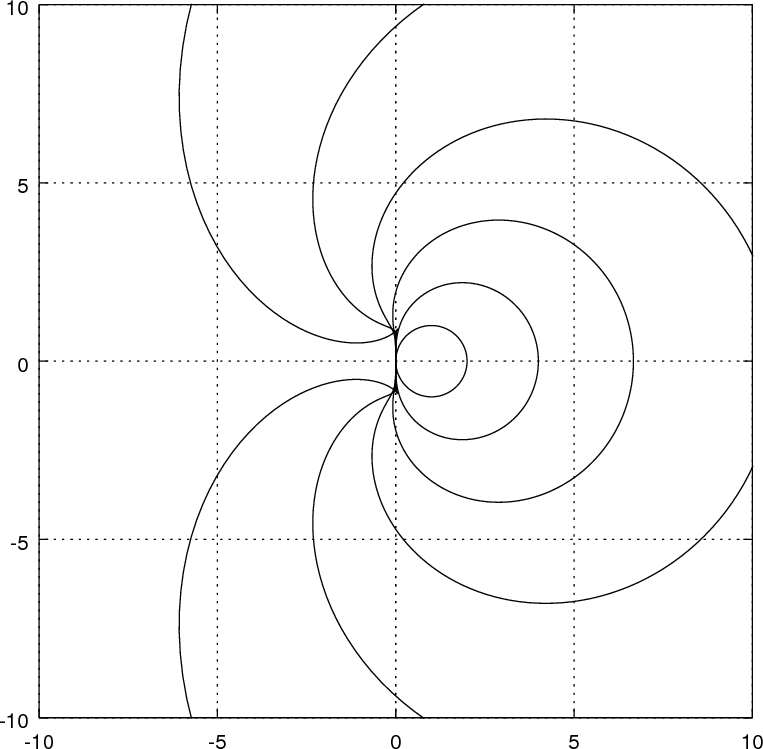
\includegraphics[width=.45\textwidth]{fig/stability-bdf.png}
  \hfill
  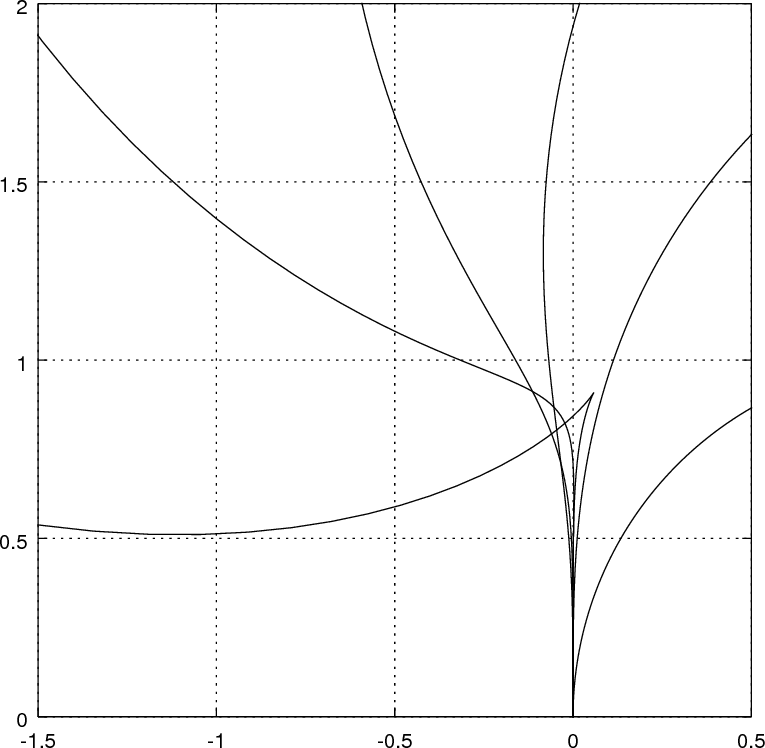
\includegraphics[width=.45\textwidth]{fig/stability-bdf-zoom.png}
  \caption{Boundaries of stability regions of BDF1 to BDF6. Unstable
    region right of the origin. Zoom on the right}
  \label{fig:bdf-stability}
\end{figure}
}

\section{Boundary Value Problems}
\frame{\tableofcontents[currentsection,hideothersubsections]}

\begin{frame}
  \begin{Definition}{bvp}
  \index{BVP|see{boundary value problem}}
  A \define{boundary value problem} (BVP) is a differential equation
  problem of the form: Find $u:[a,b]\to \R^d$, such that
  \begin{subequations}
    \label{eq:rwa:1}
    \begin{xalignat}{2}
      \label{eq:rwa:2}
      u'(t) &= f\bigl(t,u(t)\bigr)
      & t &\in (a,b) \\
      \label{eq:rwa:3}
      r\bigl(u(a), u(b)\bigr) &= 0.
    \end{xalignat}
  \end{subequations}
\end{Definition}

%%% Local Variables: 
%%% mode: latex
%%% TeX-master: "../notes"
%%% End: 

  \begin{Definition}{bvp-linear}
  A BVP~\eqref{eq:rwa:1} is called linear, if the right hand side 
  $f$ as well as the boundary conditions are linear in $u$. It has the form:
  find $u:[a,b]\to \R^d$, such that
  \begin{subequations}
    \label{eq:rwa:6}
    \begin{xalignat}{2}
      \label{eq:rwa:7}
      u'(t) &= A(t)u(t) + b(t) & \forall t &\in (a,b) \\
      \label{eq:rwa:8}
      \rwaa u(a) + \rwab u(b) &= g.
    \end{xalignat}
  \end{subequations}
\end{Definition}

%%% Local Variables: 
%%% mode: latex
%%% TeX-master: "../notes"
%%% End: 

\end{frame}

\frame{\begin{Definition}{variational-equation}
  The \define{variational equation} to the first order system of
  ODE
  \begin{gather*}
    u' = f,
  \end{gather*}
  of dimension $d$ is the linear matrix-valued system of ODE
  \begin{subequations}
  %  \label{eq:derivatives:1}
  \begin{gather}
    \label{eq:derivatives:2}
      \fundam' = \nabla_u f\bigl(t,u(t)\bigr) \fundam
  \end{gather}
  for $d\times d$ matrices $\fundam$. Here is $u$ a solution of the
  equation~\eqref{eq:awa:ode} and 
  \begin{gather*}
    \nabla_u f(t,u) =
    \begin{pmatrix}
      \tfrac{\partial f_1}{\partial u_1} & \cdots
      & \tfrac{\partial f_1}{\partial u_d} \\
      \vdots & & \vdots \\
      \tfrac{\partial f_d}{\partial u_1} & \cdots
      &  \tfrac{\partial f_d}{\partial u_d}
    \end{pmatrix}
  \end{gather*}
  is the matrix of the derivatives of $f$ with respect to the
  components of $u$. The \define{fundamental matrix}
  $\fundamental(t;t_0)$\index{Y@$\fundamental(t;t_0)$} is solution of
  the IVP to this equation with
  \begin{gather}
    \label{eq:derivatives:3}
    \fundam(t_0) = \identity.
  \end{gather}
  \end{subequations}
\end{Definition}
}
\frame{\begin{Lemma}{fundamental}
  For fundamental matrices there hold the relations
  \begin{align}
    \fundamental(t;s) &= \fundamental(s;t)^{-1}\\
    \label{eq:derivatives:4}
    \fundamental(t;r) &= \fundamental(t;s)\fundamental(s;r),
  \end{align}
  where $r,s,t$ are arbitrary real numbers, such that the solution $u$
  of the original IVP exists on the maximal interval spanned by these
  numbers.
\end{Lemma}

%%% Local Variables: 
%%% mode: latex
%%% TeX-master: "../notes"
%%% End: 
}
\frame{\begin{Theorem}{derivative}
  \index{conditioning!AWA} Let be $f(t,u)$ continuous in $t$ and
  continuously differentiable in $u$.  Then, the solution $u(t;v)$ of
  the IVP~\eqref{eq:derivatives:1} depends differentiably on the
  initial value $v$ and the derivative is given by
  \begin{gather}
    \label{eq:derivatives:5}
    \tfrac{\partial}{\partial v} u(t;v) = \fundamental(t;t_0),
  \end{gather}
  where $\fundamental(t;t_0)$ is the fundamental matrix with respect
  to the initial time $t_0$.
\end{Theorem}

}
\frame{\begin{Theorem}{derivative-f}
  Let $f(t,u)$ and $g(t,u)$ be continuous in their first and
  continuously differentiable in their second argument. Let $u$ be the
  solution of the IVP $u'=f(u)$ with $u(t_0) = u_0$. Then, the Gâteaux
  derivative of $u$ in $f$ with respect to a perturbation $g$ exists
  and there holds
  \begin{gather}
    \label{eq:derivative-f:1}
    \frac{\partial}{\partial g} u(t)
    = \int_{t_0}^t \fundamental(t;s) g\bigl(s,u(s)\bigr)\, \ds.
  \end{gather}
\end{Theorem}
%%% Local Variables:
%%% mode: latex
%%% TeX-master: "../notes"
%%% End:
}

\frame{\begin{Definition}{local-uniqueness}
  \defindex{solution!locally unique (BVP)} A solution $u(t)$ of the
  BVP~\eqref{eq:rwa:1} is called \textbf{locally unique}
  \defindex{locally unique solution (BVP)} or
  \textbf{isolated}\defindex{isolated solution}, if there is no second
  solution $v(t)$ of the BVP, which is arbitrary close to $u(t)$. In
  mathematical language: there exists an $\epsilon>0$, such that for
  any two solutions of the BVP there holds
  \begin{gather*}
    \max_{t\in [a,b]}|u(t)-v(t)| < \epsilon
    \qquad\Rightarrow\qquad
    u(t) = v(t) \quad \forall t\in [a,b].
  \end{gather*}
\end{Definition}
}
\frame{\begin{Lemma}{bvp-derivative}
  Let be $f(t,u)$ continuous in $t$ and continuously differentiable in
  $u$.  Let additionally $r(x,y)$ be continuously differentiable and
  set
  \begin{gather}
    \label{eq:rwa:9}
    \rwaa = \left.\frac{\partial r(x,y)}{\partial
        x}\right|_{x=u(a),y=u(b)},
    \qquad
    \rwab = \left.\frac{\partial r(x,y)}{\partial
        y}\right|_{x=u(a),y=u(b)}.
  \end{gather}
  Let $u(t)$ be a continuously differentiable solution of the
  BVP~\eqref{eq:rwa:1}.  Then the derivative of the boundary condition
  $r(u(a),u(b))$ with respect to the function value $u(t)$ inside the
  interval $[a,b]$ is
  \begin{gather}
    \label{eq:rwa:12}
    E(t)
    := \frac{\partial r\bigl(u(a),u(b)\bigr)}{\partial u(t)}
    = \rwaa \fundamental(a;t) + \rwab \fundamental(b;t),
  \end{gather}
  where $\fundamental(t;t_0)$ is the fundamental matrix.
\end{Lemma}
}
\frame{\begin{Definition}{local-uniqueness}
  \defindex{solution!locally unique (BVP)} A solution $u(t)$ of the
  BVP~\eqref{eq:rwa:1} is called \textbf{locally unique}
  \defindex{locally unique solution (BVP)} or
  \textbf{isolated}\defindex{isolated solution}, if there is no second
  solution $v(t)$ of the BVP, which is arbitrary close to $u(t)$. In
  mathematical language: there exists an $\epsilon>0$, such that for
  any two solutions of the BVP there holds
  \begin{gather*}
    \max_{t\in [a,b]}|u(t)-v(t)| < \epsilon
    \qquad\Rightarrow\qquad
    u(t) = v(t) \quad \forall t\in [a,b].
  \end{gather*}
\end{Definition}
}
\frame{\begin{Theorem}{bvp-stability-1}
  \index{conditioning!BVP}
  Let the assumptions of Lemma~\ref{Lemma:bvp-derivative} hold and let
  $u(t)$ be the solution of the BVP~\eqref{eq:rwa:1} with
  \begin{gather*}
    u(a) = g_a\quad \text{and} \quad u(b) = g_b.
  \end{gather*}
  Then, there holds
  \begin{gather}
    \label{eq:rwa:20}
    \frac{\partial u(t)}{\partial g_a} = E^{-1}(t) \rwaa,
    \qquad
    \frac{\partial u(t)}{\partial g_b} = E^{-1}(t) \rwab.
  \end{gather}
  In particular, the conditioning with respect to changes of size
  $\epsilon$ in the boundary conditions $g_a$ and $g_b$ is
  \begin{gather}
    \delta u(t) \le \epsilon
    \max\bigl\{\norm{E^{-1}(t) \rwaa}, \norm{E^{-1}(t)\rwab}\bigr\}.
  \end{gather}
\end{Theorem}
}
\frame{\begin{Theorem}{bvp-stability-2}
  Let $f(t,u)$ and $g(t,u)$ be continuous in $t$ and continuously
  differentiable in $u$. Then, the variation of the value $u(t)$ of
  the solution $u$ of the boundary value problem
  \begin{gather*}
    u'=f(t,u),\qquad r\bigl(u(a), u(b)\bigr)=0,
  \end{gather*}
  with respect to perturbations $f+g$ is
  \begin{gather}
    \label{eq:bvp-stability-2:1}
    \frac{\partial}{\partial g} u(t)
    = \int_{a}^b G(t,s) g\bigl(s,u(s)\bigr)\,d s,
  \end{gather}
  where
  \begin{gather}
    \label{eq:bvp-stability-2:2}
    G(t,s) =
    \begin{cases}
      -E(t)^{-1} \rwaa \fundamental(a;s) & a \le s \le t \\
      \phantom{-}E(t)^{-1} \rwab \fundamental(b;s) & t < s \le b
    \end{cases}.
  \end{gather}
\end{Theorem}

%%% Local Variables:
%%% mode: latex
%%% TeX-master: "../notes"
%%% End:
}
\frame{\begin{Definition}{bvp-linear}
  A BVP~\eqref{eq:rwa:1} is called linear, if the right hand side 
  $f$ as well as the boundary conditions are linear in $u$. It has the form:
  find $u:[a,b]\to \R^d$, such that
  \begin{subequations}
    \label{eq:rwa:6}
    \begin{xalignat}{2}
      \label{eq:rwa:7}
      u'(t) &= A(t)u(t) + b(t) & \forall t &\in (a,b) \\
      \label{eq:rwa:8}
      \rwaa u(a) + \rwab u(b) &= g.
    \end{xalignat}
  \end{subequations}
\end{Definition}

%%% Local Variables: 
%%% mode: latex
%%% TeX-master: "../notes"
%%% End: 
}
\frame{\begin{Algorithm}{single-shooting}
  The single shooting method with standard \putindex{Newton method}
  consists of the following steps:
  \begin{enumerate}
  \item Start with an initial guess $v^{(0)}\in \R^d$.
  \item For $v^{(n)}$ given, solve the IVP and the associated variation equation
    \begin{xalignat*}{2}
      \tfrac\partial{\partial t}u^{(n)}(t) &=
      f\bigl(t,u^{(n)}(t)\bigr)
      & u^{(n)}(a) &= v^{(n)},\\
      \tfrac\partial{\partial t}\fundam^{(n)}(t;a)
      &= \nabla_uf\bigl(t,u^{(n)}(t)\bigr)\fundam^{(n)}(t;a)
      &\fundam^{(n)}(a;a) &= \identity.
    \end{xalignat*}
  \item Set
    \begin{gather}
      \label{eq:rwa:14}
      v^{(n+1)} = v^{(n)}
      - \bigl(\rwaa + \rwab \fundam^{(n)}(b;a)\bigr)^{-1}
      r\bigl(v^{(n)},u^{(n)}(b)\bigr)
    \end{gather}
  \item Stop the iteration if the value
    $r\bigl(s,u(t;u_0^{(n+1)})\bigr)$ is sufficiently small,\\
    otherwise repeat from 2.
  \end{enumerate}
\end{Algorithm}

%%% Local Variables:
%%% mode: latex
%%% TeX-master: "../notes"
%%% End:
}
\frame{\begin{Algorithm}{single-shooting}
  The single shooting method with standard \putindex{Newton method}
  consists of the following steps:
  \begin{enumerate}
  \item Start with an initial guess $v^{(0)}\in \R^d$.
  \item For $v^{(n)}$ given, solve the IVP and the associated variation equation
    \begin{xalignat*}{2}
      \tfrac\partial{\partial t}u^{(n)}(t) &=
      f\bigl(t,u^{(n)}(t)\bigr)
      & u^{(n)}(a) &= v^{(n)},\\
      \tfrac\partial{\partial t}\fundam^{(n)}(t;a)
      &= \nabla_uf\bigl(t,u^{(n)}(t)\bigr)\fundam^{(n)}(t;a)
      &\fundam^{(n)}(a;a) &= \identity.
    \end{xalignat*}
  \item Set
    \begin{gather}
      \label{eq:rwa:14}
      v^{(n+1)} = v^{(n)}
      - \bigl(\rwaa + \rwab \fundam^{(n)}(b;a)\bigr)^{-1}
      r\bigl(v^{(n)},u^{(n)}(b)\bigr)
    \end{gather}
  \item Stop the iteration if the value
    $r\bigl(s,u(t;u_0^{(n+1)})\bigr)$ is sufficiently small,\\
    otherwise repeat from 2.
  \end{enumerate}
\end{Algorithm}

%%% Local Variables:
%%% mode: latex
%%% TeX-master: "../notes"
%%% End:
}
\frame{\begin{Definition}{multiple-shooting}
  Choose a partitioning of the interval $[a,b]$ such that
  \begin{gather*}
    a=t_0<t_1<t_2<\dots<t_m=b.
  \end{gather*}
  On each subinterval $I_k = [t_{k-1}, t_k]$, $k=1,\ldots,m$ define
  the IVP
  \begin{gather*}
    u_k' = f(t, u_k), \qquad u_k\bigl(t_{k-1}\bigr) = v_k,
  \end{gather*}
  The \define{multiple shooting method} consists of finding vectors
  $v_1,\dots, v_m$, such that
  \begin{xalignat*}{2}
    v_{k+1}&= u_{k}\bigl(t_{k}\bigr)& k&=1,\dots,m-1,\\
    r(v_1, u_m(b)) &= 0.
  \end{xalignat*}
  The function
  \begin{gather*}
    u(t) = u_k(t) \qquad\text{for } t\in I_k
  \end{gather*}
  is continuous, solves the ODE, and obeys the boundary conditions.
\end{Definition}

%%% Local Variables:
%%% mode: latex
%%% TeX-master: "../notes"
%%% End:
}
\frame{\begin{Definition}{multiple-shooting-newton}
  A step of Newton's method for the multiple shooting system consists
  of the update
  \begin{gather}
    \label{eq:multiple-shooting-newton:1}
    v^{(n+1)} = v^{(n)} - \nabla F(v^{(n)})^{-1} F(v^{(n)}),
  \end{gather}
  where with $v^{(n)} = [v^{(n)}_1,\dots,v^{(n)}_{m+1}]^T$ and
  \begin{gather}
    \label{eq:multiple-shooting-newton:2}
    F(v) =
    \begin{bmatrix}
      F_1(v_1, v_2)\\
      \vdots\\
      F_{m}(v_{m}, v_{m+1})\\
      F_{m+1}(v_1,v_{m+1})
    \end{bmatrix}
    ,\quad
    \nabla F(v) =
    \begin{bmatrix}
      G_1 & -\identity \\
      &\ddots & \ddots \\
      &&G_{m} & -\identity \\
      \rwaa &&& \rwab
    \end{bmatrix}.
  \end{gather}
  Here,
  \begin{xalignat*}{2}
    F_k(v_k,v_{k+1})&= u_k(t_{k}) - v_{k+1} & k&=1,\dots,m, \\
    F_{m+1}(v_1, v_{m+1}) &= r\bigl(v_1, v_{m+1}\bigr),\\
    G_k &= \fundamental(t_k;t_{k-1}) & k&=1,\dots,m.
  \end{xalignat*}
\end{Definition}
%%% Local Variables:
%%% mode: latex
%%% TeX-master: "../notes"
%%% End:
}
\frame{\begin{Definition}{multiple-shooting-multiple}
  A multi-point boundary value problem has boundary conditions of the
  form
  \begin{gather}
    \label{eq:multiple-shooting-multiple:1}
    r\bigl(u(t_0), u(t_{k_1}), u(t_{k_2}),\dots, u(t_{k_\ell})\bigr) = 0,
  \end{gather}
  with $a=t_0$, $m=k_\ell$, and $b=t_m$
  A multiple shooting method for such a problem can be designed by
  including all values $t_{k_i}$ into the partitioning of the time
  interval. The corresponding shooting function and Jacobian are
  \begin{gather}\small
    \label{eq:multiple-shooting-multiple:2}
    F(v) =
    \begin{bmatrix}
      F_1(v_1, v_2)\\
      \vdots\\
      F_{m}(v_{m}, v_{m+1})\\
      F_{m+1}(v_{1},\ldots,v_{m+1})
    \end{bmatrix}
    ,\quad
    \nabla F(v) =
    \begin{bmatrix}
      G_1 & -\identity \\
      &G_2 & -\identity \\
      &&\ddots & \ddots \\
      &&&G_{m} & -\identity \\
      \rwaa &\cdots&B_{k_i}&\cdots& \rwab
    \end{bmatrix}.
  \end{gather}
  Here,
  \begin{xalignat*}{2}
    F_k(v_k,v_{k+1})&= u_k(t_{k}) - v_{k+1} & k&=1,\dots,m, \\
    F_{m+1}(v_1,\ldots,v_{m+1}) &= r\bigl(v_1, \ldots, v_{m+1}\bigr),\\
    G_k &= \fundamental(t_k;t_{k-1}) & k&=1,\dots,m.
  \end{xalignat*}
\end{Definition}
%%% Local Variables:
%%% mode: latex
%%% TeX-master: "../notes"
%%% End:
}
\frame{\begin{Definition}{bvp-parameter}
  Given a vector $p\in \R^q$, a parameter dependent boundary value
  problem depending on $p$ has the form
  \begin{gather}
    \label{eq:bvp-parameter:1}
    \begin{split}
      u' &= f(t, u; p),\\
      r\bigl(u(a), u(b); p\bigr) &= 0.
    \end{split}
  \end{gather}
  Here, $r(\ldots) \in \R^{d+q}$ where $d$ is the dimension of the ODE system.
\end{Definition}

%%% Local Variables: 
%%% mode: latex
%%% TeX-master: "../notes"
%%% End: 
}
\frame{\begin{Definition}{multiple-shooting-parameter}
  The Jacobian of the Newton method for parameter dependent BVP is
  \begin{gather}
    \label{eq:multiple-shooting-parameter:1}
    \nabla F(v) =
    \begin{bmatrix}
      G_1 & -\identity &&& P_1\\
      &\ddots & \ddots \\
      &&G_{m} & -\identity & P_{m-1}\\
      \rwaa &&& \rwab & P_m
    \end{bmatrix}.
  \end{gather}
  Here,
  \begin{xalignat*}{2}
    P_k &= \frac{\partial u_k(t_k)}{\partial p} & k&=1,\dots,m,\\
    P_m &= \frac{\partial r(\dots)}{\partial p},\\
    G_k &= \fundamental(t_k;t_{k-1};p) & k&=1,\dots,m.
  \end{xalignat*}
\end{Definition}

%%% Local Variables:
%%% mode: latex
%%% TeX-master: "../notes"
%%% End:
}
\section{Newton and quasi-Newton methods}
\frame{\begin{Definition}{nonlinear}
  We consider two formulations of nonlinear root finding problems
  \begin{xalignat}{2}
    \label{eq:nonlinear:1}
    f(x) &= 0, & f:\R^d &\to \R^d \\
    \intertext{and}
    \label{eq:nonlinear:2}
    x &= \operatorname{argmin} F(y)
    & F: \R^d &\to \R.
  \end{xalignat}
  These two problems are equivalent by either choosing for instance
  \begin{gather*}
    f(x) = \nabla F(x)
    \qquad\text{or}\qquad
    F(x) = \abs{f(x)}.
  \end{gather*}
\end{Definition}



%%% Local Variables:
%%% mode: latex
%%% TeX-master: "../notes"
%%% End:
}
\frame{\begin{Definition}{iteration-order}
  An \putindex{iteration}
  \begin{gather*}
    x^{(k+1)} = G\left(x^{(k)}\right)
  \end{gather*}
  is said to be \textbf{convergent of order $p$}, if there holds for
  $p\ge 1$:
  \begin{gather*}
    \norm{x^{(k+1)}-x^*} \le c \norm{x^{(k)}-x^*}^p,
  \end{gather*}
  and if for $p=1$ there holds $c<1$. For $p>1$, such a method
  converges only locally, namely if $\norm{x^{(0)}-x^*}$ is
  sufficiently small, for instance
  \begin{gather*}
    \norm{x^{(0)}-x^*}^{p-1} < \frac1c.
  \end{gather*}
\end{Definition}
%%% Local Variables:
%%% mode: latex
%%% TeX-master: "../notes"
%%% End:
}
\frame{\section{Das Newton-Verfahren}

\begin{Definition}{newton-verfahren}
  Das \define{Newton-Verfahren} ist ein Iterationsverfahren zum
  Auffinden einer Nullstelle einer Funktion $f\colon \R^n\to \R^n$. Zu
  einem Startwert $x^{(0)} \in \R^n$ berechnen sich die weiteren
  Iterierten durch
  \begin{gather}
    \label{eq:newton:1}
    x^{(k+1)} = x^{(k)} - \bigl(\nabla f(x^{(k)})\bigr)^{-1} f(x^{(k)}).
  \end{gather}
\end{Definition}

\begin{Algorithmus*}{newton}{Newton-Verfahren}
  \lstinputlisting[firstline=3,lastline=9]{code/newton.py} Die
  Parameter zu dieser Funktion sind der Startwert $x$, die Funktion
  $f(x)$, die Anwendung der inversen Ableitung
  \begin{gather}
    \operatorname{Dfinv}(x,r) = \bigl(\nabla f(x)\bigr)^{-1}r,
  \end{gather}
  sowie eine Toleranz als Abbruchkriterium.
\end{Algorithmus*}
\begin{Lemma}{newton-1}
  Sei $M\subset \R^n$ konvex. Sei $f\colon M\to \R^n$ stetig differenzierbar auf $M$ und die Ableitung genüge der Lipschitz-Abschätzung
  \begin{gather}
    \norm{\nabla f(x) - \nabla f(y)} \le \gamma \norm{x-y}
    \qquad \forall x,y\in M.
  \end{gather}
  mit einer Konstanten $\gamma$. Dann gilt für alle $x,y\in M$
  \begin{gather}
    \norm{f(x)-f(y) - \nabla f(y)(x-y)}
    \le \frac\gamma2 \norm{x-y}^2.
  \end{gather}
\end{Lemma}

\begin{proof}
  Wir folgen~\cite[Hilfssatz 5.3.1]{Stoer83}.
  Sei $\phi\colon[0,1] \to \R^n$ die Hilfsfunktion definiert durch
  \begin{gather}
    \phi(t) = f\bigl(y+t(x-y)\bigr),
  \end{gather}
  so dass
  \begin{gather}
    f(x)-f(y) - \nabla f(y)(x-y) = \phi(1) - \phi(0) - \phi'(0)
    = \int_0^1 (\phi'(t)-\phi'(0))\dt,
  \end{gather}
  denn nach der Kettenregel gilt
  \begin{gather}
    \phi'(t) = \nabla f\bigl(y+t(x-y)\bigr)(x-y).
  \end{gather}
  Den Integranden schätzen wir ab durch
  \begin{align}
    \norm{\phi'(t)-\phi'(0)}
    & = \norm{\Bigl(\nabla f\bigl(y-t(x-y)\bigr) - \nabla f(y)\Bigr)(x-y)}
    \\
    & \le \norm{\nabla f\bigl(y-t(x-y)\bigr) - \nabla f(y)}\norm{(x-y)}
    \\
    & \le \gamma\,t\norm{x-y}^2.
  \end{align}
  Einsetzen ins Integral ergibt
  \begin{gather}
    \norm{f(x)-f(y) - \nabla f(y)(x-y)}
    \le \frac\gamma2 \norm{x-y}^2.
  \end{gather}
\end{proof}

\begin{Satz}{newton-konvergenz}
  Sei $M\subset \R^n$ eine offene, konvexe Menge und
  $f\colon \overline{M} \to \R^n$ stetig differenzierbar in $M$ und
  stetig auf $\overline{M}$. Die \define{Jacobi-Matrix} $\nabla f(x)$
  sei auf ganz $M$ invertierbar und es gebe Konstanten $\beta$ und
  $\gamma$, so dass für $x,y\in M$ gilt
  \begin{gather}
    \label{eq:newton:2}
    \norm{\nabla f(x) - \nabla f(y)} \le \gamma \norm{x-y},
    \qquad \norm{\bigl(\nabla f(x)\bigr)^{-1}} \le \beta.
  \end{gather}
  Gibt es dann eine Konstante $\alpha$, so dass
  \begin{align}
    \label{eq:newton:3}
    \norm{\bigl(\nabla f(x^{(0)})\bigr)^{-1} f(x^{(0)})}
    &\le \alpha\\
    h := \frac{\alpha\beta\gamma}2 &<1\\
    \overline{B_r(x^{(0)})} &\subseteq M, \qquad\text{mit } r=\frac{\alpha}{1-h},
  \end{align}
  So ist die Folge $x^{(k)}$ des Newton-Verfahrens für alle
  $k=1,\dots$ wohldefiniert und liegt in $B_r(x^{(0)})$. Ferner
  konvergiert sie quadratisch gegen einen Wert
  $x^*\in\overline{B_r(x^{(0)})}$ und es gilt
  \begin{gather}
    \label{eq:newton:4}
    \norm{x^{(k)}-x^*} \le \alpha\frac{h^{2^k-1}}{1-h^{2^k}}.
  \end{gather}
\end{Satz}

\begin{proof}
  Wir folgen~\cite[Satz 5.3.2]{Stoer83}.
  Wir zeigen zunächst induktiv für alle $k=1,\dots$, dass das
  Folgenglied $x^{(k)}$ in $B_r(x^{(0)}) \subseteq M$ liegt. Damit
  existiert dann nach Voraussetzung
  $\bigl(\nabla f(x^{(k)})\bigr)^{-1}$ und $x^{(k+1)}$ ist
  wohldefiniert. Zur Verankerung bemerken wir, dass offensichtlich
  $x^{(0)}\in B_r(x^{(0)})$ und $x^{(1)}$ nach
  Voraussetzung~\eqref{eq:newton:3}. Nach der Verfahrensvorschrift
  können wir abschätzen:
  \begin{align}
    \norm{x^{(k+1)} - x^{(k)}}
    & = \norm{\bigl(\nabla f(x^{(k)})\bigr)^{-1} f(x^{(k)})}\\
    & \le \beta \norm{f(x^{(k)})}\\
    & = \beta \norm{f(x^{(k)}) - f(x^{(k-1)}) - \nabla f(x^{(k)})(x^{(k)}-x^{(k-1)})},
  \end{align}
  wobei wir die letzte Zeile aus der Multiplikation der
  Verfahrensvorschrift mit $\nabla f$ gewonnen haben. Hierauf wenden
  wir nun \slideref{Lemma}{newton-1} an und bekommen die quadratische
  Konvergenz, wenn der Abstand zweier Folgenglieder einmal klein genug
  ist:
  \begin{gather}
    \label{eq:newton:5}
    \norm{x^{(k+1)} - x^{(k)}}
    \le \frac{\beta\gamma}2 \norm{x^{(k)} - x^{(k-1)}}^2.
  \end{gather}
  Es bleibt zu zeigen, dass die Folge in $B_r(x^{(0)})$ bleibt. Dazu
  zeigen wir per Induktion, dass
  \begin{gather}
    \label{eq:newton:6}
    \norm{x^{(k+1)} - x^{(k)}} \le \alpha h^{2^k-1}.
  \end{gather}
  Für $k=0$ folgt $\norm{x^{(1)} - x^{(0)}} \le \alpha$ direkt
  aus~\eqref{eq:newton:3}. Für den Induktionsschritt benutzen wir
  unsere Konvergenzabschätzung~\eqref{eq:newton:5}:
  \begin{gather}
    \norm{x^{(k+1)} - x^{(k)}}
    \le \frac{\beta\gamma}2 \norm{x^{(k)} - x^{(k-1)}}^2
    \le \frac{\beta\gamma}2 (\alpha h^{2^{k-1}-1})^2
    = \frac{\alpha\beta\gamma}2 \alpha h^{2^k-2}
    = \alpha h^{2^k-1}.
  \end{gather}
  Nun können wir mit einer Teleskopsumme abschätzen
  \begin{align}
    \norm{x^{(k+1)} - x^{(0)}}
    &\le \sum_{j=0}^k \norm{x^{(j+1)} - x^{(j)}}\\
    & \le \alpha (1+h+h^3+h^7+\dots+h^{2^k-1})\\
    &<\frac\alpha{1-h} = r,
  \end{align}
  Aus~\eqref{eq:newton:6} folgt mit dieser Abschätzung, dass $x^{(k)}$
  Cauchy Folge ist und durch Grenzübergang die
  Abschätzung~\eqref{eq:newton:4}.
\end{proof}

\section{Abstiegsverfahren und Globalisierung}

\begin{intro}
  Die lokale Konvergenz ist beim Newtonverfahren ein großes Hindernis
  für die Anwendung. Wählt man den Startwert nicht im Einzugsbereich
  einer Nullstelle, so divergiert das Verfahren. Der Einzugsbereich,
  wie er sich aus dem Konvergenzsatz ergibt, ist dabei oft sehr klein
  und daher schwer zu finden.

  Ziel dieses Abschnitts ist daher, eine Modifikation des
  Newton-Verfahrens zu finden, die den Konvergenzbereich aufweitet,
  idealerweise sogar globale Konvergenz erzeugt. Solche Modifikationen
  findet man unter der Bezeichnung \define{Globalisierung}.
\end{intro}

\begin{Definition}{anstiegskegel}
  Sei $g\colon \R^n\to \R$ stetig differenzierbar. Dann definieren wir
  den Kegel positiven Anstiegs zum Parameter $\gamma$ als
  \begin{gather}
    S_\gamma(x) = \bigl\{ s\in\R^n \big|
    \norm{s} = 1 \;\wedge \;
    \nabla g(x)\cdot s \ge \gamma\norm{\nabla g(x)}
    \bigr\}.
  \end{gather}
  Die Richtung des steilsten Anstiegs im Punkt $x$ ist $\nabla g(x)$.
\end{Definition}

\begin{todo}
  Umgebung ``remark''.
\end{todo}
Da es sich um normierte Vektoren handelt, ist die Menge $S_\gamma(x)$
eigentlich kein Kegel, sondern eine Kugel in der Einheitssphäre mit
Zentrum im normierten Gradienten und Radius $\arccos \gamma$. Zusammen
mit den Skalierungsfaktoren, die unten eingeführt werden,
repräsentiert sie aber einen Kegel.


\begin{Lemma}{abstieg-reduktion}
  Sei $g\colon\R^n\to\R$ stetig differenzierbar und in einem Punkt
  $y\in\R^n$ gelte $\nabla g(y) \neq 0$. Dann gibt es eine Umgebung
  $U(y)$ und $\lambda>0$, so dass für alle $x\in U(y)$,
  $s\in S_\gamma(x)$ und $\mu\in [0,\lambda]$ gilt
  \begin{gather}
    g(x-\mu s) \le g(x) - \frac{\mu\gamma}4 \norm{\nabla g(y)}.
  \end{gather}
\end{Lemma}

\begin{proof}
  Wir definieren zunächst eine Umgebung um $y$ auf der sich die
  Gradienten nicht zu sehr unterscheiden:
  \begin{gather}
    \label{eq:newton:8}
    U_1(y) = \left\{
      x\in\R^n \middle| \;\norm{\nabla g(x)-\nabla g(y)} \le \frac\gamma4 \norm{\nabla g(y)}
      \right\}.
    \end{gather}
    Eine zweite Umgebung ist so gewählt, dass dort der Abstiegskegel
    in einem größeren Abstiegskegel im Punkt $y$ enthalten ist:
    \begin{gather}
      U_2(y) = \left\{
        x\in\R^n \middle| S_\gamma(x) \subseteq S_{\nicefrac\gamma2}(y)\right\}.
    \end{gather}

    Wähle nun $\lambda>0$, so dass
    \begin{gather}
      \overline{B_{2\lambda}(y)}\subseteq U_1(y) \cap U_2(y).
    \end{gather}
    und $U(y) = B_\lambda(y)$. Dann zeigen wir nun die Aussage für
    alle $x\in U(y)$, $s\in S_\gamma(x)$ und $\mu\in[0,\lambda]$. Nach
    dem Mittelwertsatz existiert $\theta\in(0,1)$ so dass
    \begin{gather}
      g(x)-g(x-\mu s) = \mu \nabla g(x-\theta\mu s)s.
    \end{gather}
    Wir formen weiter um:
    \begin{align}
      \nabla g(x-\theta\mu s)s
      &= \bigl(\nabla g(x-\theta\mu s) - \nabla g(y)\bigr)s + \nabla g(y)s\\
      &\ge -\frac{\gamma}4 \norm{\nabla g(y)}\norm{s} + \nabla g(y)s\\
      &\ge -\frac{\gamma}4 \norm{\nabla g(y)} + \frac\gamma2 \norm{\nabla g(y)}\\
      & \ge \frac\gamma4 \norm{\nabla g(y)}.
    \end{align}
\end{proof}

\begin{todo}
  Reihenfolge vertauschen  
\end{todo}

\begin{Definition}{abstiegsverfahren}
  Ein \define{Abstiegsverfahren} für eine stetig differenzierbare
  Funktion $g\colon \R^n\to\R$ ist eine Iterationsvorschrift aus den
  folgenden Schritten: gegeben $x^{(k)}$,
  \begin{enumerate}
  \item wähle $\gamma_k>\gamma>0$ und eine Abstiegsrichtung
    $s^{(k)} \in S_{\gamma_k}(x^{(k)})$.
  \item Wähle eine Schrittweite $\alpha_k>0$ und setze
    \begin{gather}
      x^{(k+1)} = x^{(k)} - \alpha_k s^{(k)},
    \end{gather}
    so dass die \define{Reduktionsbedingung}
    \begin{gather}
      \label{eq:newton:7}
      g\bigl(x^{(k+1)}\bigr)
      \le g\bigl(x^{(k)}\bigr) - \frac{\gamma_k\alpha_k}{4}\norm{\nabla g(x^{(k)})}
    \end{gather}
    gilt.
  \end{enumerate}
\end{Definition}

\begin{remark}
  Lemma \slideref{Lemma}{abstieg-reduktion} stellt sicher, dass es in
  jedem Schritt ein positives $\alpha_k$ gibt, das die Bedingung
  erfüllt.
\end{remark}

\begin{Beispiel*}{steepest-descent}{Verfahren des steilsten Abstiegs}
  Sei der Vektor $x^{(k)} \in\R^n$ gegeben, dann wähle
  $s^{(k)} = \nabla g(x^{(k)})$. Die Schrittweite $\alpha_k$ wird aus
  der eindimensionalen Minimierungsaufgabe (auch \define{line search}
  genannt)
  \begin{gather}
    \alpha_k = \operatorname*{argmin}_{\alpha>0}
    g\bigl(x^{(k)} - \alpha s^{(k)}\bigr)
  \end{gather}
  bestimmt. Danach setze
  \begin{gather}
    x^{(k+1)} = x^{(k)} - \alpha_k s^{(k)}.
  \end{gather}
\end{Beispiel*}

\begin{Satz}{abstieg-haeufung}
  Sei $g\colon \R^n\to \R$ und $x^{(0)} \in\R^n$ so gewählt, dass die Menge
  \begin{gather}
    K = \Bigl\{x\in\R^n \; \Big| \; g(x) \le g\bigl(x^{(0)}\bigr) \Bigr\}
  \end{gather}
  kompakt und $g$ stetig differenzierbar auf einer Umgebung von $K$
  ist. Dann besitzt die Folge $\{x^{(k)}\}$ des Abstiegsverfahrens
  mindestens einen Häufungspunkt in $K$. Gilt zusätzlich in der
  Umgebung eines Häufungspunkts $\gamma_k \ge \gamma>0$, so existiert
  $\alpha$, so dass $\alpha_k \ge \alpha>0$ gewählt werden kann. In
  diesem Fall ist der Häufungspunkt ein stationärer Punkt von $g$.
\end{Satz}

\begin{proof}
  Da die Folge monoton fällt, bleibt sie in $K$ und hat der
  Kompaktheit wegen mindestens einen Häufungspunkt $x^*$. Wir benennen
  nun ebenfalls mit $\{x^{(k)}\}$ ebenfalls eine Teilfolge, die gegen diesen
  Häufungspunkt konvergiert.

  Wir machen die Widerspruchsannahme, dass $x^*$ kein stationäre Punkt von $g$ ist, also
  \begin{gather}
    \nabla g(x^*) \neq 0.
  \end{gather}

  Wir bemerken, dass nach Voraussetzung $S_{\gamma_k}(x^*) \subseteq S_\gamma(x^*)$ gilt.
  Nun gibt es nach \slideref{Lemma}{abstieg-reduktion} eine Umgebung
  $U(x^*)$ und eine Zahl $\lambda>0$, so dass für alle $\mu\in[0,\lambda]$ gilt:
  \begin{gather}
    g(x-\mu s) \le g(x) - \mu \frac\gamma4\norm{\nabla g(x^*)}.
  \end{gather}
  Daraus folgt, dass zu jedem $\alpha_k \le \lambda$ die
  Reduktionsbedingung~\eqref{eq:newton:7} erfüllt ist und
  dementsprechend die Bedingung $\alpha_k\ge\alpha$ für
  $\alpha\le\lambda$ erfüllt werden kann.

  Sei nun $k_0$ gewählt, so dass $x^{(k)}\in U(x^*)$ für alle
  $k\ge k_0$. Dann gilt nach der Konstruktion von $U(x^*)$
  in~\eqref{eq:newton:8}, dass
  \begin{gather}
    \norm{\nabla g(x^{(k)})} \ge \norm{\nabla g(x^{*})} - \norm{\nabla g(x^{(k)}) - \nabla g(x^{*})}
    \ge \left(1-\frac\gamma4\right)  \norm{\nabla g(x^{*})}.
  \end{gather}
  Es gilt also
  \begin{gather}
    g(x^{k+1}) \le g(x^{k}) - \frac34 \alpha \norm{\nabla g(x^{*})}.
  \end{gather}
  Daraus folgt im Widerspruch zur Stetigkeit die Konvergenz
  $g(x^{(k)}) \to -\infty$, Es muss also $\nabla g(x^{*})=0$ gelten,
  $x^*$ ist also ein stationärer Punkt von $g$.
\end{proof}

\begin{remark}
  Der vorherige besteht aus zwei Teilen. Die Existenz eines
  Häufungspunktes wird unter einer der allgemeinen Bedingung
  getroffen, dass die Menge $K$ kompakt ist, also eine Abstiegsfolge
  nicht ins unendliche konvergieren kann. Diese Bedingung ist oft
  recht leicht nachzuprüfen. Insbesondere steht die Existenz mehrerer
  Häufungspunkte nicht im Widerspruch zu den Annahmen, so dass das
  Verfahren auch dann wenigstens einen davon findet.

  Die weiteren Bedingungen, die sicherstellen, dass es sich bei einem
  Häufungspunkt um einen stationären Punkt handelt, sind lokal in
  einer Umgebung eines solchen gestellt. An diesem Punkt sind die
  Folgen $\gamma_k$ und $\alpha_k$ nur sehr abstrakt fixiert. Wir
  zeigen nun, dass die Folge der $\alpha_k$ im Verfahren des steilsten
  Abstiegs die Bedingung erfüllt. Als zweite Anwendung von allgemeinen
  Abstiegsverfahren stellen wir dann das Newton-Verfahren mit
  Schrittweitensteuerung vor.
\end{remark}

\begin{Korollar}{abstieg-haeufung}
  Beim Verfahren des steilsten Abstiegs sind die Folgen $\gamma_k$ und
  $\alpha_k$ so gewählt, das \slideref{Satz}{abstieg-haeufung} gilt.
\end{Korollar}

\begin{proof}
  Da die Abstiegsrichtungen immer gleich dem (negativen) Gradienten
  sind, gilt $\gamma_k \equiv 1$. Für die Folge $\alpha_k$ zeigen wir
  nich die Beschränktheit durch $\alpha$. Stattdessen bemerken wir mit
  $\lambda$ aus \slideref{Lemma}{abstieg-reduktion}:
  \begin{align}
    g(x^{(k+1)})
    &= \min_{\alpha>0} g\left(x^{(k+1)}-\alpha s^{(k)}\right)\\
    &\le g(x^{(k)}-\lambda s^{(k)})\\
    &\le g(x^{(k)}) - \frac{\lambda}4 \norm{\nabla g(x^*)}.
  \end{align}
  Auch hier schließen wir, dass die Folge divergiert wenn die Punkte konvergieren.
\end{proof}

\begin{Lemma}{newton-abstieg}
  Sei $f\colon \R^n\to \R^n$ stetig differenzierbar und
  $g(x) = \norm{f(x)}_2^2$.  Dann sind die Suchrichtungen des Newton-Verfahrens
  \begin{gather}
    s^{(k)} = \frac{d^{(k)}}{\norm{d^{(k)}}_2},
    \qquad d^{(k)} = \bigl(\nabla f(x^{(k)})\bigr)^{-1}f(x^{(k)})
  \end{gather}
  Abstiegsrichtungen für $g(x)$ und es gilt
  \begin{gather}
    s^{(k)} \in S_\gamma\bigl(x^{(k)}\bigr),
    \qquad
    \gamma = \frac{1}{\cond_2(\nabla f(x^{(k)}))}
  \end{gather}
\end{Lemma}

\begin{proof}
  Es gilt (Nachrechnen!)
  \begin{gather}
    \nabla g(x) = 2 f(x)^T\nabla f(x).
  \end{gather}
  Daher ist
  \begin{align}
    \frac{\nabla g(x) s}{\norm{\nabla g(x)}_2}
    &= \frac{f(x)^T \nabla f(x) \bigl(\nabla f(c)\bigr)^{-1} f(x)}
      {\norm{f(x)^T\nabla f(x)}_2\norm{\bigl(\nabla f(c)\bigr)^{-1} f(x)}}_2\\
    &\ge \frac{\norm{f(x)}^2_2}{\norm{f(x)}_2\norm{\nabla f(x)}_2\norm{\bigl(\nabla f(c)\bigr)^{-1}}_2\norm{f(x)}_2}\\
    &= \frac1{\cond_2(\nabla f)}.
  \end{align}
\end{proof}

\begin{Korollar}{newton-abstieg}
  Das modifizierte Newton-Verfahren
  \begin{gather}
    x^{(k+1)} = x^{(k)} - \alpha_k \bigl(\nabla f(x^{(k)})\bigr)^{-1} f(x^{(k)})
  \end{gather}
  ist ein Abstiegsverfahren, wenn $\alpha_k$ so gewählt ist, dass die
  Reduktionsbedingung gilt.
\end{Korollar}

\begin{remark}
  Man kann nun zum Beispiel auch das Newton-Verfahren mit line search
  ausführen, um globale Konvergenzeigenschaften zu erzielen. Es gilt
  dann zunächst die Existenz von Häufungspunkten. In der Nähe eines
  solchen gilt aber natürlich, dass line search nicht schlechter
  konvergiert, als das normale Newton-Verfahren, woraus dann dort
  wieder die quadratische Konvergenz gefolgert werden kann.

  Wir betrachten stattdessen die folgende, einfachere Variante, die
  mit minimaler Modifikation ein global konvergierendes Verfahren
  ergibt.
\end{remark}

\begin{Definition}{newton-stepsize}
  Das Newton-Verfahren mit \define{Schrittweitensteuerung} berechnet iterativ
  $x^{(k+1)}\in \R^n$ aus $x^{(k)}\in \R^n$ in folgenden Schritten
  \begin{enumerate}
  \item Berechne $d^{(k)} = \bigl(\nabla f(x^{(k)})\bigr)^{-1}f(x^{(k)})$
  \item Berechne die kleinste ganze Zahl $j$, so dass
    \begin{multline}
      \norm*{f(x^{(k)}-2^{-j} d^{(k)})}_2^2
      \le \norm*{f(x^{(k)})}_2^2
      \\- 2^{-j} \frac{1}{4\cond_2(\nabla f(x^{(k)}))}
      \norm*{f^T\bigl(x^{(k)}\bigr)\nabla f\bigl(x^{(k)}\bigr)}_2
    \end{multline}
    \item Setze $x^{(k+1)}=x^{(k)}-2^{-j} d^{(k)}$
  \end{enumerate}
\end{Definition}

\begin{remark}
  Der Algorithmus benötigt viele zusätzliche Berechnungen, wie die von
  $\gamma_k$ oder $\nabla g$. Für die praktische Anwendung lässt er
  sich vereinfachen. Dazu beobachten wir zunächst, dass
  Bedingung~\eqref{eq:newton:7} dazu dient, eine hinreichende
  Kontraktion in der Nähe eines Häufungspunkts sicherzustellen. Die
  Existenz eines solchen kann bereits aus
  \begin{gather}
    g\bigl(x^{k+1}\bigr) < g\bigl(x^{k}\bigr)
  \end{gather}
  gefolgert werden. Umgekehrt wird, wenn die Funktion $f$ die
  Bedingungen des Konvergenzsatzes \slideref{Satz}{newton-konvergenz}
  erfüllt, in der Nähe eines Fixpunktes ohnehin $j=0$ gelten. Wir
  ersetzen daher die komplizierte Bedingung durch die wesentlich
  einfachere: sei $j$ die kleinste nichtnegative ganze Zahl, so dass
  \begin{gather}
    \norm*{f\bigl(x^{k} - 2^{-j} d^{(k)}\bigr)}_2^2 < \norm*{f\bigl(x^{k}\bigr)}_2^2.
  \end{gather}
  Es gibt in der Literatur weitere Heuristiken zur Wahl der
  Schrittweite im Newton-Verfahren, die man unter dem Stichwort \glqq
  Globalisierung\grqq{} findet. Hier wollen wir uns mit dieser
  besonders einfachen und gleichzeitig effektiven Variante begnügen.
\end{remark}

\begin{Algorithmus*}{newton-stepsize}{Newton-Verfahren mit Schrittweitensteuerung}
    \lstinputlisting[firstline=3,lastline=18]{code/newton-stepsize.py}
\end{Algorithmus*}

\begin{remark}
  Dieser Abschnitt gibt Hinweise darauf, wie das Newton-Verfahren
  modifiziert werden kann und trotzdem Konvergenz erhalten wird. Neben
  der Schrittweitensteuerung kommen hier insbesondere approximative
  Berechnungen der Ableitung in Frage. Diese werden dann oft als
  \define{Quasi-Newton-Verfahren} bezeichnet, konvergieren in der
  Regel nur von erster Ordnung, sind aber of viel effizienter als das
  Newton-Verfahren selbst.
\end{remark}

%%% Local Variables:
%%% mode: latex
%%% TeX-master: "main"
%%% End:
}
\frame{\begin{Theorem*}{newton-kantorovich}{Newton-Kantorovich}
  Let $f: \R^d \to \R^d$ be differentiable with
  \begin{xalignat}2
    \label{eq:newton-kantorovich:1}
    \norm{\nabla f(x) - \nabla f(y)}
    & \le L \norm{x-y} & x,y&\in \R^d,
    \\
    \label{eq:newton-kantorovich:2}
    \norm{\left(\nabla f\left(x^{(0)}\right)\right)^{-1}} &\le M.
  \end{xalignat}
  Then, if
  \begin{gather}
    \label{eq:newton-kantorovich:3}
    \beta_0 := LM \norm{f\left(x^{(0)}\right)} \le \frac12,
  \end{gather}
  the Newton method converges to a root of $f(x)$. If furthermore
  $\beta_0 < 1/2$, this convergence is quadratic.
\end{Theorem*}

%%% Local Variables:
%%% mode: latex
%%% TeX-master: "../notes"
%%% End:
}
\frame{\begin{Definition}{gradient-method}
  The \define{gradient method} for finding minimizers of a nonlinear
  functional $F(x)$ reads:  given an initial value $x^{(0)}$, compute
  iterates $x^{(k)}$, $k=1,2,\ldots$ by the rule
  \begin{gather}
    \label{eq:gradient-method:1}
    \begin{split}
      d^{(k)} &= -\nabla F(x^{(k)}),
      \\
      \alpha_k &=
      \operatorname*{argmin}_{\gamma>0} F\left(x^{(k)} + \gamma d^{(k)}\right)
      \\
      x^{(k+1)} &= x^{(k)} + \alpha_k d^{(k)}.
    \end{split}
  \end{gather}
  The minimization process used to compute $\alpha_k$, also called
  \define{line search}, is one-dimensional
  and therefore simple. It may be replaced by a heuristic choice of
  $\alpha_k$.
\end{Definition}

%%% Local Variables:
%%% mode: latex
%%% TeX-master: "../notes"
%%% End:
}
\frame{\begin{Definition}{gradient-method}
  The \define{gradient method} for finding minimizers of a nonlinear
  functional $F(x)$ reads:  given an initial value $x^{(0)}$, compute
  iterates $x^{(k)}$, $k=1,2,\ldots$ by the rule
  \begin{gather}
    \label{eq:gradient-method:1}
    \begin{split}
      d^{(k)} &= -\nabla F(x^{(k)}),
      \\
      \alpha_k &=
      \operatorname*{argmin}_{\gamma>0} F\left(x^{(k)} + \gamma d^{(k)}\right)
      \\
      x^{(k+1)} &= x^{(k)} + \alpha_k d^{(k)}.
    \end{split}
  \end{gather}
  The minimization process used to compute $\alpha_k$, also called
  \define{line search}, is one-dimensional
  and therefore simple. It may be replaced by a heuristic choice of
  $\alpha_k$.
\end{Definition}

%%% Local Variables:
%%% mode: latex
%%% TeX-master: "../notes"
%%% End:
}
\frame{\begin{Definition}{predictor-corrector}
  Assume a pair of time stepping schemes, one explicit, one implicit,
  \begin{align*}
    \hat y_{k} &= \hat \Phi(y_{k-1}) \\
    y_k &= \Phi(y_{k-1},y_{k}),
  \end{align*}
  we can use $\hat y_k$ as initial value for the Newton iteration for
  $y_k$. In an extreme case, we let
  \begin{gather*}
    y_k = \Phi(y_{k-1},\hat y_{k}),
  \end{gather*}
  without any further iteration.
\end{Definition}

%%% Local Variables:
%%% mode: latex
%%% TeX-master: "../notes"
%%% End:
}
\frame{\begin{Definition}{newton-line-search}
  The \define{Newton method with line search}\index{line search} for
  finding the root of the nonlinear equation $f(x) = 0$ reads: given
  an initial value $x^{(0)}$, compute iterates $x^{(k)}$,
  $k=1,2,\ldots$ by the rule
  \begin{gather}
    \label{eq:newton-line-search:1}
    \begin{split}
      J &= \nabla f\left(x^{(k)}\right),
      \\
       J d^{(k)} &= f(x^{(k)}),
      \\
      \alpha_k &= \operatorname*{argmin} f(x^{(k)} - \alpha d^{(k)})\\
      x^{(k+1)} &= x^{(k)} - \alpha_k d^{(k)}.
    \end{split}
  \end{gather}
\end{Definition}

%%% Local Variables:
%%% mode: latex
%%% TeX-master: "../notes"
%%% End:
}
\frame{\begin{Lemma}{downhill}
  Let $F: \R^d \to \R$ be continuously differentiable. For a given
  point $x$, assume $\nabla F = \nabla F(x) \neq 0$.  Then, there is a
  constant $\lambda > 0$ such that for any
  $s\in \mathcal S_\gamma(\nabla F(x))$ and any
  $0 \le \mu \le \lambda$ there holds
  \begin{gather}
    \label{eq:downhill:1}
    F(x-\mu s) \le F(x) - \frac{\gamma\mu}4 \abs{\nabla F(x)}.
  \end{gather}
  In particular, a positive scaling factor $\mu$ for the descent method can
  always be found.
\end{Lemma}
%%% Local Variables: 
%%% mode: latex
%%% TeX-master: "../notes"
%%% End: 
}
\frame{\begin{Definition}{newton-step-size}
  The \define{Newton method with step size control} for finding the
  root of the nonlinear equation $f(x) = 0$ reads: given an initial
  value $x^{(0)}$, compute iterates $x^{(k)}$, $k=1,2,\ldots$ by the
  rule
  \begin{gather}
    \label{eq:newton-step-size:1}
    \begin{split}
      J &= \nabla f\left(x^{(k)}\right),
      \\
      J d^{(k)} &= f(x^{(k)}),
      \\
      x^{(k+1)} &= x^{(k)} - 2^{-j} d^{(k)}.
    \end{split}
  \end{gather}
  Here, $j$ is the smallest integer number, such that
  \begin{gather}
    \label{eq:newton-step-size:2}
    f(x^{(k)} - 2^{-j} d^{(k)}) < f(x^{(k)}),
  \end{gather}
  for practical purposes.
\end{Definition}

%%% Local Variables:
%%% mode: latex
%%% TeX-master: "../notes"
%%% End:
}

\section{Finite Differences}
\frame{\tableofcontents[currentsection,hideothersubsections]}

\frame{\begin{Definition}{partitioning}
  On a time interval $I = [0,T]$, we define a partitioning in $n$
  subintervals, also known as \textbf{time steps}.\defindex{time step}
  Here we choose the following notation:
%  \begin{figure}[tp]
  \begin{center}
    \small
    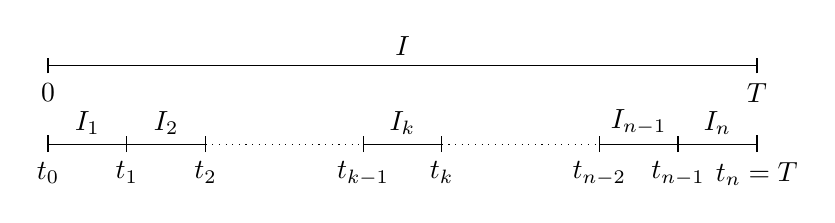
\begin{tikzpicture}
      \draw(0,1) -- node [anchor=south]{$I$} (9,1);
      \draw[thick](0,.9) node[anchor=north]{$0$} -- (0,1.1);
      \draw[thick](9,.9) node[anchor=north]{$T$} --(9,1.1);

      \draw(0,0)-- node [anchor=south]{$I_1$}(1,0);
      \draw(1,0)-- node [anchor=south]{$I_2$}(2,0);
      \draw(4,0)-- node [anchor=south]{$I_k$}(5,0);
      \draw(7,0)-- node [anchor=south]{$I_{n-1}$}(8,0);
      \draw(8,0)-- node [anchor=south]{$I_{n}$}(9,0);
      \draw[dotted](2,0)--(4,0);
      \draw[dotted](5,0)--(7,0);
      \draw[thick](0,-.1) node[anchor=north]{$t_0$} -- (0,.12);
      \draw(1,-.1) node[anchor=north]{$t_1$} --(1,.1);
      \draw(2,-.1) node[anchor=north]{$t_2$} --(2,.1);
      \draw(4,-.1) node[anchor=north]{$t_{k-1}$} --(4,.1);
      \draw(5,-.1) node[anchor=north]{$t_k$} --(5,.1);
      \draw(7,-.1) node[anchor=north]{$t_{n-2}$} --(7,.1);
      \draw(8,-.1) node[anchor=north]{$t_{n-1}$} --(8,.1);
      \draw[thick](9,-.1) node[anchor=north]{$t_n=T$} --(9,.12);
    \end{tikzpicture}
  \end{center}
%    \caption{Partition of the interval $I=[0,T]$ in subintervals $I_1,\dots,I_n$.}
%    \label{fig:explicit:schritte}
%  \end{figure}
  The time steps $I_k = [t_{k-1},t_{k}]$ have the step size
  $h_k = t_{k} - t_{k-1}$.  A partitioning in $n$ time steps implies
  $t_n = T$.  The term $k$-th time step is used for both the interval
  $I_k$ and for the point in time $t_k$, but it should always be clear
  through context which one is meant.

  Very often, we will consider evenly spaced time steps, in which case
  we denote the step size by $h$ and $h_k=h$ for all $k$.
\end{Definition}

%%% Local Variables:
%%% mode: latex
%%% TeX-master: "../notes"
%%% End:
}
\frame{\begin{Definition}{bvp-second}
  Given an interval $I=[a,b]$, find a function
  \begin{gather}
    \label{eq:bvp-second:3}
    u\in V = \Bigl\{u\in C^2(a,b) \cap C[a,b]
	\;\Big|\; u(a) = u(b) = 0 \Bigr\},
  \end{gather}
  such that for a differential operator of second order as defined
  above and a right hand side $f\in C[a,b]$ there holds
  \begin{gather}
    \label{eq:bvp-second:2}
    Lu = f.
  \end{gather}
\end{Definition}
%%% Local Variables:
%%% mode: latex
%%% TeX-master: "../notes"
%%% End:
}
\frame{\begin{Definition*}{difference-operators}{Finite differences}
  In order to approximate first derivatives of a function $u$, we introduce
  the operators
  \begin{xalignat}{2}
    \label{eq:difference-operators:1a}
    &\text{Forward difference }& D^+_h u(x)&= \frac{u(x+h)-u(x)}h, \\
    \label{eq:difference-operators:1b}
    &\text{Backward difference }& D^-_h u(x)&= \frac{u(x)-u(x-h)}h, \\
    \label{eq:difference-operators:1c}
    &\text{Central difference }& D^c_h u(x)&= \frac{u(x+h)-u(x-h)}{2h}.
  \end{xalignat}
  For second derivatives we introduce the
  \begin{xalignat}{2}
    \label{eq:difference-operators:2}
    &\text{3-point stencil }& D^2_h u(x)
    &= \frac{u(x+h) - 2 u(x) + u(x-h)}{h^2}.
  \end{xalignat}
\end{Definition*}
%%% Local Variables:
%%% mode: latex
%%% TeX-master: "../notes"
%%% End:
}
\frame{\begin{Lemma}{fd-consistency}
  The difference operators have the following consistency orders
  \begin{align}
    \label{eq:fd-consistency:1}
    \abs{u'(x)-D^+_hu(x)} & \le c h \\
    \label{eq:fd-consistency:2}
    \abs{u'(x)-D^h_hu(x)} & \le c h \\
    \label{eq:fd-consistency:3}
    \abs{u'(x)-D^c_hu(x)} & \le c h^2 \\
    \label{eq:fd-consistency:4}
    \abs{u''(x)-D^2_hu(x)} & \le c h^2
  \end{align}
\end{Lemma}

%%% Local Variables: 
%%% mode: latex
%%% TeX-master: "../notes"
%%% End: 
}
\frame{\begin{Lemma}{fd-consistency}
  The difference operators have the following consistency orders
  \begin{align}
    \label{eq:fd-consistency:1}
    \abs{u'(x)-D^+_hu(x)} & \le c h \\
    \label{eq:fd-consistency:2}
    \abs{u'(x)-D^h_hu(x)} & \le c h \\
    \label{eq:fd-consistency:3}
    \abs{u'(x)-D^c_hu(x)} & \le c h^2 \\
    \label{eq:fd-consistency:4}
    \abs{u''(x)-D^2_hu(x)} & \le c h^2
  \end{align}
\end{Lemma}

%%% Local Variables: 
%%% mode: latex
%%% TeX-master: "../notes"
%%% End: 
}
\frame{\chapter{Second Order Boundary Value Problems}

\section{2nd order two-point boundary value problems}

\begin{intro}
  We have already seen, that boundary value problems have very
  different stability properties than initial value
  problems. Here, we will discuss a special class of boundary value
  problems of the form
  \begin{gather}
    \label{eq:bvp-second:1}
    -u''(x) + \beta(x) u'(x) + \gamma(x)u(x) = f(x),
    \qquad u(a) = u_a,
    \quad u(b) = u_b.
  \end{gather}

  In order to make this problem more amenable to mathematical
  investigation, we introduce the set
  \begin{gather*}
    \mathcal B =
    \Bigl\{ u\in C^2(a,b) \cap C[a,b]
    \;\Big|\; u(a) = u_a\;\wedge\; u(b) = u_b
    \Bigr\}.
  \end{gather*}

  Then, we can see the left hand side of the differential equation as
  a differential operator applied to $u$ and thus mapping $\mathcal B$
  to the set of continuous functions. Namely, we define
  \begin{gather}
    \label{eq:fd:2}
    \begin{split}
      L: \mathcal B &\to C[a,b] \\
      u & \mapsto -u'' + \beta u' + \gamma u.
    \end{split}
  \end{gather}
  In addition, we would like to simplify our life and get rid of the
  inhomogeneous boundary values $u_a$ and $u_b$. To this end, let
  \begin{gather*}
    u_B(x) = u_a \frac{b-x}{b-a} + u_b \frac{x-a}{b-a},
  \end{gather*}
  and introduce the new function $u_0 = u+u_B$. Then, $u_0$ solves
  the boudnary value problem
  \begin{multline*}
    -u_0''(x) + \beta(x) u'(x) + \gamma(x)u(x) = f(x) -
    \beta(x)\frac{u_b-u_a}{b-a} - \gamma(x)u_B(x),
    \\ u(a) =  u(b) = 0.
  \end{multline*}
  Thus, it is sufficient to consider the boundary value problem
\end{intro}

\begin{Definition}{bvp-second}
  Given an interval $I=[a,b]$, find a function
  \begin{gather}
    \label{eq:bvp-second:3}
    u\in V = \Bigl\{u\in C^2(a,b) \cap C[a,b]
	\;\Big|\; u(a) = u(b) = 0 \Bigr\},
  \end{gather}
  such that for a differential operator of second order as defined
  above and a right hand side $f\in C[a,b]$ there holds
  \begin{gather}
    \label{eq:bvp-second:2}
    Lu = f.
  \end{gather}
\end{Definition}
%%% Local Variables:
%%% mode: latex
%%% TeX-master: "../notes"
%%% End:


\begin{remark}
  This definition exhibits a major change in paradigm. Before, we
  considered a differential equation as an equation which determines
  the derivative of a function in a point. Now, we are looking at a
  linear system of equations, albeit one, which is not of finite
  dimension. This paradigm change will be essential when we consider
  partial differential equations in future semesters.
  
  On the other hand, the equality in equation~\eqref{eq:bvp-second:2}
  is understood point-wise, such that in fact nothing but our point of
  view has changed.
\end{remark}

\begin{intro}
  Again, we subdivide the interval $I= [a,b]$ into subintervals, but
  the subdivision does not involve IVP solvers on subintervals, but
  much more like in the original subdivision in
  Definition~\ref{Definition:partitioning}, the the solution will only
  be defined at the partitioning points $t_k$, $k=0,\dots,n$.
  
  Thus, like with one-step and multistep methods we will have values
  $y_0, y_1,\dots, y_n$, but the sequence has a defined end at $y_n$
  due to the right boundary of the interval.

  While one-step methods directly discretize the Volterra integral
  equation in order to compute a solution at every new step,
  \textbf{finite difference methods} discretize the differential
  equation on the whole interval at once and then solve the resulting
  discrete (finite-dimensional) system of equations.

  We have accompished the first step and decided that instead of
  function values in every point of the interval $I$, we only
  approximate $u(t_k)$ in the points of the partition. What is left is
  the definition of the discrete operator representing the equation.
\end{intro}

\begin{Definition*}{difference-operators}{Finite differences}
  In order to approximate first derivatives of a function $u$, we introduce
  the operators
  \begin{xalignat}{2}
    \label{eq:difference-operators:1a}
    &\text{Forward difference }& D^+_h u(x)&= \frac{u(x+h)-u(x)}h, \\
    \label{eq:difference-operators:1b}
    &\text{Backward difference }& D^-_h u(x)&= \frac{u(x)-u(x-h)}h, \\
    \label{eq:difference-operators:1c}
    &\text{Central difference }& D^c_h u(x)&= \frac{u(x+h)-u(x-h)}{2h}.
  \end{xalignat}
  For second derivatives we introduce the
  \begin{xalignat}{2}
    \label{eq:difference-operators:2}
    &\text{3-point stencil }& D^2_h u(x)
    &= \frac{u(x+h) - 2 u(x) + u(x-h)}{h^2}.
  \end{xalignat}
\end{Definition*}
%%% Local Variables:
%%% mode: latex
%%% TeX-master: "../notes"
%%% End:


\begin{remark}
  The 3-point stencil is the product of forward and backward
  difference operators.
  \begin{gather*}
    D^2_h u(x) = D^+_hu(x)D^-_hu(x) = D^-_hu(x)D^+_hu(x).
  \end{gather*}
  For simplicity, we only present finite differences of uniform
  subdivisions. Nevertheless, the definition of the operators can be
  extended easily to $h$ changing between intervals.
\end{remark}

\begin{Lemma}{fd-consistency}
  The difference operators have the following consistency orders
  \begin{align}
    \label{eq:fd-consistency:1}
    \abs{u'(x)-D^+_hu(x)} & \le c h \\
    \label{eq:fd-consistency:2}
    \abs{u'(x)-D^h_hu(x)} & \le c h \\
    \label{eq:fd-consistency:3}
    \abs{u'(x)-D^c_hu(x)} & \le c h^2 \\
    \label{eq:fd-consistency:4}
    \abs{u''(x)-D^2_hu(x)} & \le c h^2
  \end{align}
\end{Lemma}

%%% Local Variables: 
%%% mode: latex
%%% TeX-master: "../notes"
%%% End: 

\begin{Lemma}{fd-consistency}
  The difference operators have the following consistency orders
  \begin{align}
    \label{eq:fd-consistency:1}
    \abs{u'(x)-D^+_hu(x)} & \le c h \\
    \label{eq:fd-consistency:2}
    \abs{u'(x)-D^h_hu(x)} & \le c h \\
    \label{eq:fd-consistency:3}
    \abs{u'(x)-D^c_hu(x)} & \le c h^2 \\
    \label{eq:fd-consistency:4}
    \abs{u''(x)-D^2_hu(x)} & \le c h^2
  \end{align}
\end{Lemma}

%%% Local Variables: 
%%% mode: latex
%%% TeX-master: "../notes"
%%% End: 


\begin{proof}
  We begin to show consistency of the first two operators by Taylor
  expansion: for some $\xi\in(x,x+h)$, there holds
  \begin{align*}
    u'(x) - D^+_h u(x) &= u'(x) - \frac{u(x+h) - u(x)}h \\
    &= u'(x) - \frac{u(x)+h u'(x) + \tfrac{h^2}{2} u''(\xi) - u(x)}h
    \\
    &= \tfrac h2 u''(\xi).
  \end{align*}
  The same computation can be applied to $D^-_h u(x)$. It is clear
  that we need an additional symmetry argument for te other two,
  otherwise their consistency order would be lower. Therefore, we
  follow the line of argument that we introduced in
  Lemma~\ref{Lemma:lmm-bramble-hilbert}, and which here reads: a
  difference operator $D^\alpha_h$ approximating a derivative of order
  $\alpha$ is consistent of order $p$, if and only if it is exact for all
  polynomials of degree $p+\alpha-1$. We realize this by computing the
  Taylor polynomial $p(h)$ of degree $p+\alpha-1$ and the remainder term
  involving $u^{(p+\alpha)}(\xi)$. Then,
  \begin{gather*}
    D^\alpha_h u(x) = \frac{p(h)+\frac{h^{\alpha+p}}{(\alpha+p)!}u^{(p+\alpha)}(\xi)}{h^\alpha}.
  \end{gather*}
  Now we employ that the formula is exact for $p(h)$ and thus
  \begin{gather*}
    u^{(\alpha)}(x) - D^\alpha_h u(x)
    = \frac{h^p}{(\alpha+p)!}u^{(p+\alpha)}(\xi).
  \end{gather*}
  We now write
  \begin{gather*}
    p(\xi) = a_0 + a_1 (\xi-x) + a_2 (\xi-x)^2 + a_3 (\xi-x)^3 + \cdots
  \end{gather*}
  The central difference $D^c_h$ is exact for linear polynomials,
  since ti evaluates to zero for a constant and $D^c_h (\xi-x) =
  1$. But additionally, we observe
  \begin{gather*}
    \frac{d}{d\xi} (\xi-x)^2 \Bigr|_{\xi=x}
    = D^c_h (\xi-x)^2 \Bigr|_{\xi=x}= 0.
  \end{gather*}
  Thus, the central difference is exact for polynomials of degree 2
  and consistent of second order.

  For the 3-point stencil, we observe that $D^2_h u(x)=0$ for any
  function $u$ such that $u(x+h) - u(x-h) = u(x)$, in particular any
  odd polynomial in $\xi-x$. Furthermore,
  \begin{gather*}
    D^2_h  (\xi-x)^2 \Bigr|_{\xi=x}= \frac{h^2-0+h^2}{h^2}
    = 2 = \frac{d^2}{d\xi^2} (\xi-x)^2
  \end{gather*}
\end{proof}

\begin{remark}
  When applied to the equation $u'=f(t,u)$ the solutions obtained by
  forward and backward differences correspond to the explicit and
  implicit Euler methods, respectively.
\end{remark}

\chapter{Second Order Boundary Value Problems}

\section{2nd order two-point boundary value problems}

\begin{intro}
  We have already seen, that boundary value problems have very
  different stability properties than initial value
  problems. Here, we will discuss a special class of boundary value
  problems of the form
  \begin{gather}
    \label{eq:bvp-second:1}
    -u''(x) + \beta(x) u'(x) + \gamma(x)u(x) = f(x),
    \qquad u(a) = u_a,
    \quad u(b) = u_b.
  \end{gather}

  In order to make this problem more amenable to mathematical
  investigation, we introduce the set
  \begin{gather*}
    \mathcal B =
    \Bigl\{ u\in C^2(a,b) \cap C[a,b]
    \;\Big|\; u(a) = u_a\;\wedge\; u(b) = u_b
    \Bigr\}.
  \end{gather*}

  Then, we can see the left hand side of the differential equation as
  a differential operator applied to $u$ and thus mapping $\mathcal B$
  to the set of continuous functions. Namely, we define
  \begin{gather}
    \label{eq:fd:2}
    \begin{split}
      L: \mathcal B &\to C[a,b] \\
      u & \mapsto -u'' + \beta u' + \gamma u.
    \end{split}
  \end{gather}
  In addition, we would like to simplify our life and get rid of the
  inhomogeneous boundary values $u_a$ and $u_b$. To this end, let
  \begin{gather*}
    u_B(x) = u_a \frac{b-x}{b-a} + u_b \frac{x-a}{b-a},
  \end{gather*}
  and introduce the new function $u_0 = u+u_B$. Then, $u_0$ solves
  the boudnary value problem
  \begin{multline*}
    -u_0''(x) + \beta(x) u'(x) + \gamma(x)u(x) = f(x) -
    \beta(x)\frac{u_b-u_a}{b-a} - \gamma(x)u_B(x),
    \\ u(a) =  u(b) = 0.
  \end{multline*}
  Thus, it is sufficient to consider the boundary value problem
\end{intro}

\begin{Definition}{bvp-second}
  Given an interval $I=[a,b]$, find a function
  \begin{gather}
    \label{eq:bvp-second:3}
    u\in V = \Bigl\{u\in C^2(a,b) \cap C[a,b]
	\;\Big|\; u(a) = u(b) = 0 \Bigr\},
  \end{gather}
  such that for a differential operator of second order as defined
  above and a right hand side $f\in C[a,b]$ there holds
  \begin{gather}
    \label{eq:bvp-second:2}
    Lu = f.
  \end{gather}
\end{Definition}
%%% Local Variables:
%%% mode: latex
%%% TeX-master: "../notes"
%%% End:


\begin{remark}
  This definition exhibits a major change in paradigm. Before, we
  considered a differential equation as an equation which determines
  the derivative of a function in a point. Now, we are looking at a
  linear system of equations, albeit one, which is not of finite
  dimension. This paradigm change will be essential when we consider
  partial differential equations in future semesters.
  
  On the other hand, the equality in equation~\eqref{eq:bvp-second:2}
  is understood point-wise, such that in fact nothing but our point of
  view has changed.
\end{remark}

\begin{intro}
  Again, we subdivide the interval $I= [a,b]$ into subintervals, but
  the subdivision does not involve IVP solvers on subintervals, but
  much more like in the original subdivision in
  Definition~\ref{Definition:partitioning}, the the solution will only
  be defined at the partitioning points $t_k$, $k=0,\dots,n$.
  
  Thus, like with one-step and multistep methods we will have values
  $y_0, y_1,\dots, y_n$, but the sequence has a defined end at $y_n$
  due to the right boundary of the interval.

  While one-step methods directly discretize the Volterra integral
  equation in order to compute a solution at every new step,
  \textbf{finite difference methods} discretize the differential
  equation on the whole interval at once and then solve the resulting
  discrete (finite-dimensional) system of equations.

  We have accompished the first step and decided that instead of
  function values in every point of the interval $I$, we only
  approximate $u(t_k)$ in the points of the partition. What is left is
  the definition of the discrete operator representing the equation.
\end{intro}

\begin{Definition*}{difference-operators}{Finite differences}
  In order to approximate first derivatives of a function $u$, we introduce
  the operators
  \begin{xalignat}{2}
    \label{eq:difference-operators:1a}
    &\text{Forward difference }& D^+_h u(x)&= \frac{u(x+h)-u(x)}h, \\
    \label{eq:difference-operators:1b}
    &\text{Backward difference }& D^-_h u(x)&= \frac{u(x)-u(x-h)}h, \\
    \label{eq:difference-operators:1c}
    &\text{Central difference }& D^c_h u(x)&= \frac{u(x+h)-u(x-h)}{2h}.
  \end{xalignat}
  For second derivatives we introduce the
  \begin{xalignat}{2}
    \label{eq:difference-operators:2}
    &\text{3-point stencil }& D^2_h u(x)
    &= \frac{u(x+h) - 2 u(x) + u(x-h)}{h^2}.
  \end{xalignat}
\end{Definition*}
%%% Local Variables:
%%% mode: latex
%%% TeX-master: "../notes"
%%% End:


\begin{remark}
  The 3-point stencil is the product of forward and backward
  difference operators.
  \begin{gather*}
    D^2_h u(x) = D^+_hu(x)D^-_hu(x) = D^-_hu(x)D^+_hu(x).
  \end{gather*}
  For simplicity, we only present finite differences of uniform
  subdivisions. Nevertheless, the definition of the operators can be
  extended easily to $h$ changing between intervals.
\end{remark}

\begin{Lemma}{fd-consistency}
  The difference operators have the following consistency orders
  \begin{align}
    \label{eq:fd-consistency:1}
    \abs{u'(x)-D^+_hu(x)} & \le c h \\
    \label{eq:fd-consistency:2}
    \abs{u'(x)-D^h_hu(x)} & \le c h \\
    \label{eq:fd-consistency:3}
    \abs{u'(x)-D^c_hu(x)} & \le c h^2 \\
    \label{eq:fd-consistency:4}
    \abs{u''(x)-D^2_hu(x)} & \le c h^2
  \end{align}
\end{Lemma}

%%% Local Variables: 
%%% mode: latex
%%% TeX-master: "../notes"
%%% End: 

\begin{Lemma}{fd-consistency}
  The difference operators have the following consistency orders
  \begin{align}
    \label{eq:fd-consistency:1}
    \abs{u'(x)-D^+_hu(x)} & \le c h \\
    \label{eq:fd-consistency:2}
    \abs{u'(x)-D^h_hu(x)} & \le c h \\
    \label{eq:fd-consistency:3}
    \abs{u'(x)-D^c_hu(x)} & \le c h^2 \\
    \label{eq:fd-consistency:4}
    \abs{u''(x)-D^2_hu(x)} & \le c h^2
  \end{align}
\end{Lemma}

%%% Local Variables: 
%%% mode: latex
%%% TeX-master: "../notes"
%%% End: 


\begin{proof}
  We begin to show consistency of the first two operators by Taylor
  expansion: for some $\xi\in(x,x+h)$, there holds
  \begin{align*}
    u'(x) - D^+_h u(x) &= u'(x) - \frac{u(x+h) - u(x)}h \\
    &= u'(x) - \frac{u(x)+h u'(x) + \tfrac{h^2}{2} u''(\xi) - u(x)}h
    \\
    &= \tfrac h2 u''(\xi).
  \end{align*}
  The same computation can be applied to $D^-_h u(x)$. It is clear
  that we need an additional symmetry argument for te other two,
  otherwise their consistency order would be lower. Therefore, we
  follow the line of argument that we introduced in
  Lemma~\ref{Lemma:lmm-bramble-hilbert}, and which here reads: a
  difference operator $D^\alpha_h$ approximating a derivative of order
  $\alpha$ is consistent of order $p$, if and only if it is exact for all
  polynomials of degree $p+\alpha-1$. We realize this by computing the
  Taylor polynomial $p(h)$ of degree $p+\alpha-1$ and the remainder term
  involving $u^{(p+\alpha)}(\xi)$. Then,
  \begin{gather*}
    D^\alpha_h u(x) = \frac{p(h)+\frac{h^{\alpha+p}}{(\alpha+p)!}u^{(p+\alpha)}(\xi)}{h^\alpha}.
  \end{gather*}
  Now we employ that the formula is exact for $p(h)$ and thus
  \begin{gather*}
    u^{(\alpha)}(x) - D^\alpha_h u(x)
    = \frac{h^p}{(\alpha+p)!}u^{(p+\alpha)}(\xi).
  \end{gather*}
  We now write
  \begin{gather*}
    p(\xi) = a_0 + a_1 (\xi-x) + a_2 (\xi-x)^2 + a_3 (\xi-x)^3 + \cdots
  \end{gather*}
  The central difference $D^c_h$ is exact for linear polynomials,
  since ti evaluates to zero for a constant and $D^c_h (\xi-x) =
  1$. But additionally, we observe
  \begin{gather*}
    \frac{d}{d\xi} (\xi-x)^2 \Bigr|_{\xi=x}
    = D^c_h (\xi-x)^2 \Bigr|_{\xi=x}= 0.
  \end{gather*}
  Thus, the central difference is exact for polynomials of degree 2
  and consistent of second order.

  For the 3-point stencil, we observe that $D^2_h u(x)=0$ for any
  function $u$ such that $u(x+h) - u(x-h) = u(x)$, in particular any
  odd polynomial in $\xi-x$. Furthermore,
  \begin{gather*}
    D^2_h  (\xi-x)^2 \Bigr|_{\xi=x}= \frac{h^2-0+h^2}{h^2}
    = 2 = \frac{d^2}{d\xi^2} (\xi-x)^2
  \end{gather*}
\end{proof}

\begin{remark}
  When applied to the equation $u'=f(t,u)$ the solutions obtained by
  forward and backward differences correspond to the explicit and
  implicit Euler methods, respectively.
\end{remark}

\chapter{Second Order Boundary Value Problems}

\section{2nd order two-point boundary value problems}

\begin{intro}
  We have already seen, that boundary value problems have very
  different stability properties than initial value
  problems. Here, we will discuss a special class of boundary value
  problems of the form
  \begin{gather}
    \label{eq:bvp-second:1}
    -u''(x) + \beta(x) u'(x) + \gamma(x)u(x) = f(x),
    \qquad u(a) = u_a,
    \quad u(b) = u_b.
  \end{gather}

  In order to make this problem more amenable to mathematical
  investigation, we introduce the set
  \begin{gather*}
    \mathcal B =
    \Bigl\{ u\in C^2(a,b) \cap C[a,b]
    \;\Big|\; u(a) = u_a\;\wedge\; u(b) = u_b
    \Bigr\}.
  \end{gather*}

  Then, we can see the left hand side of the differential equation as
  a differential operator applied to $u$ and thus mapping $\mathcal B$
  to the set of continuous functions. Namely, we define
  \begin{gather}
    \label{eq:fd:2}
    \begin{split}
      L: \mathcal B &\to C[a,b] \\
      u & \mapsto -u'' + \beta u' + \gamma u.
    \end{split}
  \end{gather}
  In addition, we would like to simplify our life and get rid of the
  inhomogeneous boundary values $u_a$ and $u_b$. To this end, let
  \begin{gather*}
    u_B(x) = u_a \frac{b-x}{b-a} + u_b \frac{x-a}{b-a},
  \end{gather*}
  and introduce the new function $u_0 = u+u_B$. Then, $u_0$ solves
  the boudnary value problem
  \begin{multline*}
    -u_0''(x) + \beta(x) u'(x) + \gamma(x)u(x) = f(x) -
    \beta(x)\frac{u_b-u_a}{b-a} - \gamma(x)u_B(x),
    \\ u(a) =  u(b) = 0.
  \end{multline*}
  Thus, it is sufficient to consider the boundary value problem
\end{intro}

\input{definitions/bvp-second}

\begin{remark}
  This definition exhibits a major change in paradigm. Before, we
  considered a differential equation as an equation which determines
  the derivative of a function in a point. Now, we are looking at a
  linear system of equations, albeit one, which is not of finite
  dimension. This paradigm change will be essential when we consider
  partial differential equations in future semesters.
  
  On the other hand, the equality in equation~\eqref{eq:bvp-second:2}
  is understood point-wise, such that in fact nothing but our point of
  view has changed.
\end{remark}

\begin{intro}
  Again, we subdivide the interval $I= [a,b]$ into subintervals, but
  the subdivision does not involve IVP solvers on subintervals, but
  much more like in the original subdivision in
  Definition~\ref{Definition:partitioning}, the the solution will only
  be defined at the partitioning points $t_k$, $k=0,\dots,n$.
  
  Thus, like with one-step and multistep methods we will have values
  $y_0, y_1,\dots, y_n$, but the sequence has a defined end at $y_n$
  due to the right boundary of the interval.

  While one-step methods directly discretize the Volterra integral
  equation in order to compute a solution at every new step,
  \textbf{finite difference methods} discretize the differential
  equation on the whole interval at once and then solve the resulting
  discrete (finite-dimensional) system of equations.

  We have accompished the first step and decided that instead of
  function values in every point of the interval $I$, we only
  approximate $u(t_k)$ in the points of the partition. What is left is
  the definition of the discrete operator representing the equation.
\end{intro}

\input{definitions/difference-operators}

\begin{remark}
  The 3-point stencil is the product of forward and backward
  difference operators.
  \begin{gather*}
    D^2_h u(x) = D^+_hu(x)D^-_hu(x) = D^-_hu(x)D^+_hu(x).
  \end{gather*}
  For simplicity, we only present finite differences of uniform
  subdivisions. Nevertheless, the definition of the operators can be
  extended easily to $h$ changing between intervals.
\end{remark}

\input{definitions/fd-consistency}
\input{theorems/fd-consistency}

\begin{proof}
  We begin to show consistency of the first two operators by Taylor
  expansion: for some $\xi\in(x,x+h)$, there holds
  \begin{align*}
    u'(x) - D^+_h u(x) &= u'(x) - \frac{u(x+h) - u(x)}h \\
    &= u'(x) - \frac{u(x)+h u'(x) + \tfrac{h^2}{2} u''(\xi) - u(x)}h
    \\
    &= \tfrac h2 u''(\xi).
  \end{align*}
  The same computation can be applied to $D^-_h u(x)$. It is clear
  that we need an additional symmetry argument for te other two,
  otherwise their consistency order would be lower. Therefore, we
  follow the line of argument that we introduced in
  Lemma~\ref{Lemma:lmm-bramble-hilbert}, and which here reads: a
  difference operator $D^\alpha_h$ approximating a derivative of order
  $\alpha$ is consistent of order $p$, if and only if it is exact for all
  polynomials of degree $p+\alpha-1$. We realize this by computing the
  Taylor polynomial $p(h)$ of degree $p+\alpha-1$ and the remainder term
  involving $u^{(p+\alpha)}(\xi)$. Then,
  \begin{gather*}
    D^\alpha_h u(x) = \frac{p(h)+\frac{h^{\alpha+p}}{(\alpha+p)!}u^{(p+\alpha)}(\xi)}{h^\alpha}.
  \end{gather*}
  Now we employ that the formula is exact for $p(h)$ and thus
  \begin{gather*}
    u^{(\alpha)}(x) - D^\alpha_h u(x)
    = \frac{h^p}{(\alpha+p)!}u^{(p+\alpha)}(\xi).
  \end{gather*}
  We now write
  \begin{gather*}
    p(\xi) = a_0 + a_1 (\xi-x) + a_2 (\xi-x)^2 + a_3 (\xi-x)^3 + \cdots
  \end{gather*}
  The central difference $D^c_h$ is exact for linear polynomials,
  since ti evaluates to zero for a constant and $D^c_h (\xi-x) =
  1$. But additionally, we observe
  \begin{gather*}
    \frac{d}{d\xi} (\xi-x)^2 \Bigr|_{\xi=x}
    = D^c_h (\xi-x)^2 \Bigr|_{\xi=x}= 0.
  \end{gather*}
  Thus, the central difference is exact for polynomials of degree 2
  and consistent of second order.

  For the 3-point stencil, we observe that $D^2_h u(x)=0$ for any
  function $u$ such that $u(x+h) - u(x-h) = u(x)$, in particular any
  odd polynomial in $\xi-x$. Furthermore,
  \begin{gather*}
    D^2_h  (\xi-x)^2 \Bigr|_{\xi=x}= \frac{h^2-0+h^2}{h^2}
    = 2 = \frac{d^2}{d\xi^2} (\xi-x)^2
  \end{gather*}
\end{proof}

\begin{remark}
  When applied to the equation $u'=f(t,u)$ the solutions obtained by
  forward and backward differences correspond to the explicit and
  implicit Euler methods, respectively.
\end{remark}

\input{definitions/fd}

\input{definitions/fd-example}

\begin{remark}
  Like our view to the continuous boundary value problem has changed,
  the discrete one is now a fully coupled linear system which has to
  be solved by methods of linear algebra, not by time stepping
  anymore. In fact, we have $n+1$ variables $y_0,\dots, y_n$ and $n+1$
  equations, such that here existence and uniqueness of solutions are
  equivalent.
\end{remark}

\input{definitions/fd-matrix}

\begin{remark}
  The first and last row of the matrix $L_h$ are redundant, since they
  simply say $y_0 = y_n = 0$. They can be eliminated, such that we
  obtain the reduced system
  \begin{gather}
    \label{eq:fd:8}
    L_h y =
    \begin{pmatrix}
      \lambda_1 & \nu_1\\
      \mu_2 & \lambda_2 & \ddots \\
      & \ddots & \ddots & \nu_{n-2} \\
      &&\mu_{n-1}& \lambda_{n-1}
    \end{pmatrix}
    \begin{pmatrix}
      y_1\\\vdots\\y_{n-1}
    \end{pmatrix}
    =
    \begin{pmatrix}
      f_1 \\\vdots\\f_{n-1}
    \end{pmatrix} = f_h.
  \end{gather}
  In this form, the operator $L_h$ is consistent with $L$ in the sense
  that it only describes the differential operator, not the boundary
  values. Therefore, we will use this form in our further analysis.

  When it comes to implementation, both versions have their
  merits. Obviously, the new operator involves less unknowns. On the
  other hand, the discretization with boundary unknowns is more
  straight-forward.
\end{remark}

\section{Existence, stability, and convergence}

\begin{intro}
  Since the solution of the discretized boundary value problem is a
  problem in linear algebra, we have to study properties of the matrix
  $L_h$. The shortest and most elegant way to prove stability is
  through the properties of M-matrices, which we present here very
  shortly. We are not dwelling on this approach too long, since it is
  sufficient for stability, but by far not necessary and constrained
  to low order methods.

  The fact that $L_h$ is an M-matrix requires some knowledge of
  irreducible weakly diagonal dominant matrices, which the author
  considers as outdated as the whole concept of m-matrices. We will
  just quote this result without proof.
\end{intro}

\input{definitions/m-matrix}

\begin{Lemma}{m-matrix-fd1}
  The matrix $L_h$ defined above is an M-matrix provided that
  \begin{gather}
    \label{eq:fd:3}
    \gamma_k \ge 0, % > -\frac2{h^2},
    \qquad
    \abs{\beta_k} < \frac2h.
  \end{gather}
\end{Lemma}

\begin{proof}
  It is clear that these two conditions are sufficient for the first
  M-matrix property. The proof of positivity of the inverse is based
  on irreducible diagonal dominance, which is too long and too
  specialized for these notes.
\end{proof}

\begin{remark}
  The finite element method provides much more powerful to deduce
  solvability and stability of the discrete problem.
\end{remark}

\input{theorems/m-matrix-inverse}

\begin{proof}
  Let $x\in \R^n$ and $y = A^{-1} x$. Then,
  \begin{align*}
    \abs{y_i} & = \abs{\sum c_{ij} x_j} \\
    & \le \sum c_{ij} \abs{x_j} \\
    & \le \norm{x}_\infty \sum c_{ij} v_j.
  \end{align*}
  Thus,
  \begin{gather*}
    \abs{y_i} \le  \norm{x}_\infty \bigl(A^{-1} v\bigr)_i
    = \norm{x}_\infty \bigl(A^{-1} Aw\bigr)_i \le \norm{x}_\infty \abs{w_i}.
  \end{gather*}
  Taking the maximum over all $i$, we obtain
  \begin{gather*}
    \norm{A^{-1}}_\infty = \sup_{u\in
      \R^n}\frac{\norm{A^{-1}u}_\infty}{\norm{u}_\infty}
    \le \norm{w}_\infty.
  \end{gather*}
\end{proof}

\input{theorems/fd-stability}

\begin{proof}
  Take the function
  \begin{gather*}
    p(x) = (x-a)(b-x) = -x^2+(a+b)x-ab,
  \end{gather*}
  with derivatives $p'(x) = a+b-2x$ and $p''(x) = -2$, and a maximum
  of $(b-a)^2/4$ at $x=(a+b)/2$. Choose the values $p_k = p(x_k)$. By
  consistency, we have and $k=1,\dots,n-1$
  \begin{gather*}
    (L_h p)_k \ge 2 - \beta_k\abs{b-a} + \gamma_k \abs{b-a}^2
    \ge 2-\delta.
  \end{gather*}
  Thus, the vector with entries $w_k = p_k/(2-\delta)$ can be used to
  bound the inverse of $L_h$ by Lemma~\ref{Lemma:m-matrix-inverse}.
\end{proof}

\begin{remark}
  The assumptions of the previous theorem involve two sets of
  conditions on the parameters $\beta_k$ and
  $\gamma_k$. Condition~\eqref{eq:fd:1} is actually a condition on the
  continuous problem. The condition on $\gamma_k$ is indeed necessary,
  as will be seen when we study partial differential equations. The
  condition on $\beta_k$ is not necessary in this form, but a better
  estimate again requires far advanced analysis.

  The other set of conditions relates the coefficients to the mesh
  size. Again, the condition on $\beta_k$ can be avoided as seen in
  the next example. The condition on $\gamma_k$ is already implied by
  $-\gamma_k \le (b-a)^2$, which is a small restriction compared
  to~\eqref{eq:fd:1}, as soon as the partition has 3 interior
  points. Thus, it is not crucial.
\end{remark}

\input{definitions/upwind}
\input{theorems/fd-convergence}

\begin{proof}
  We apply the difference operator $L_h$ to $u$ (as the vector of
  function values in the points $t_k$) and $y$ to obtain
  \begin{gather*}
    L_h(u-y) = (L_h - L) u + Lu - L_h y = \tau + f - f = \tau,
  \end{gather*}
  where $\tau = (\tau_1,\dots,\tau_{n-1})^T$ is the vector, which
  measures the consistency error  $(L_h-L) u$ in each $t_k$. The
  entries $\tau_k$ are bounded by $c h^p$ by the consistency estimate.
  For the error, there holds
  \begin{gather*}
    u-y = L_h^{-1} L_h(u-y) =  L_h^{-1} \tau.
  \end{gather*}
  Using the stability assumption, we obtain
  \begin{gather*}
    \norm{u-y}_\infty \le \norm{L_h^{-1}}_\infty \norm{\tau}_\infty
    \le c h^p,
  \end{gather*}
  where the constant $c$ depends on $\norm{L_h^{-1}}_\infty$ and the
  constant in the consistency estimate, but not on $h$.
\end{proof}

\begin{remark}
  Finite differences can be generalized to higher order by extending
  the stencils by more than one point to the left and right of the
  current point. Whenever we add two points to the symmetric
  difference formulas, we can gain two orders of consistency.
  \begin{gather*}
    \underbrace{\bullet\quad
      \underbrace{\bullet\quad
        \underbrace{\bullet\quad\phantom{\bullet}\quad\bullet}_{u'+\mathcal O(h^2)}
        \quad\bullet}_{u'+\mathcal O(h^4)}
      \quad\bullet}_{u'+\mathcal O(h^6)}
    \qquad\qquad
    \underbrace{\bullet\quad
      \underbrace{\bullet\quad
        \underbrace{\bullet\quad\bullet\quad\bullet}_{u''+\mathcal O(h^2)}
        \quad\bullet}_{u''+\mathcal O(h^4)}
      \quad\bullet}_{u''+\mathcal O(h^6)}
  \end{gather*}
  Similarly, we can define one-sided difference formulas, which get us
  close to multistep methods. The matrices generated by these formulas
  are not M-matrices anymore, although you can show for the 4th order
  formula for the second derivative that it yields a product of two
  M-matrices. While this rescues the theory in a particular instance,
  M-matrices do not provide a theoretical framework for general high
  order finite differences anymore.

  Very much like the starting procedures for high order multistep
  methods, high order finite differences cause problems at the
  boundaries. Here, the formulas must be truncated and for instance be
  replaced by one-sided formulas of equal order.
  
  All these issues motivate the study of different discretization
  methods in the next course.
\end{remark}

\section{The Laplacian and harmonic functions}

\begin{intro}
  The two-point boundary value problem has a natural extension to
  higher dimensions. There, we deal with partial derivatives
  $\frac{\partial}{\partial x}$, $\frac{\partial}{\partial y}$, and
  $\frac{\partial}{\partial z}$. As an outlook towards topics
  discussed in classes on partial differential equations and their
  numerical analysis, we close these notes by a short introduction at
  hand of examples.
\end{intro}

\begin{Definition}{laplace-equation}
  the \define{Laplacian} in two (three) space dimensions is the sum of
  the second partial derivatives
  \begin{gather}
    \label{eq:fd:10}
    \Delta u = \frac{\partial^2}{\partial x^2}u
    + \frac{\partial^2}{\partial y^2}u
    \left(+ \frac{\partial^2}{\partial z^2}u\right)
    = \operatorname{div}(\nabla u)
  \end{gather}
  The \define{Laplace equation} is the partial differential equation
  \begin{gather}
    \label{eq:fd:11}
    -\Delta u = 0.
  \end{gather}
  The \define{Poisson equation} is the partial differential equation
  \begin{gather}
    \label{eq:fd:9}
    -\Delta u = f.
  \end{gather}
  Solutions to the Laplace equations are called \define{harmonic functions}.
\end{Definition}

\subsection{Properties of harmonic functions}

\begin{Theorem*}{mean-value}{Mean-value formula for harmonic functions}
  Let $u\in C^2(\Omega)$ be a solution to the Laplace equation. Then,
  $u$ has the mean value property
  \begin{gather}
    \label{eq:mean-value:1}
    u(\mathbf x) = \frac1{r^{d-1}\omega(d)}
    \int_{\partial B_r(\mathbf x)} u(\mathbf y) \,ds,
  \end{gather}
  where $\partial B_r(\mathbf x) \subset \Omega$ is the sphere of
  radius $r$ around $\mathbf x$ and $\omega(d)$ is the volume of the
  unit sphere in $\R^d$.
\end{Theorem*}

\begin{proof}
  First, we rescale the problem to
  \begin{gather*}
    \Phi(r) = \frac1{r^{d-1}\omega(d)}
    \int_{\partial B_r(\mathbf x)} u(\mathbf y) \,ds
    = \frac1{\omega(d)} \int_{\partial B_1(0)} u(\mathbf x+r\mathbf z) \,ds.
  \end{gather*}
  Then, we notice that
  \begin{align*}
    \Phi'(r)
    &= \frac1{\omega(d)} \int_{\partial B_1(0)}
      \nabla u(\mathbf x+r\mathbf z)\cdot \mathbf z \,ds_z\\
    &= \frac1{r^{d-1}\omega(d)} \int_{\partial B_r(\mathbf x)}
      \nabla u(\mathbf y)\cdot\frac{\mathbf y-\mathbf x}{r} \,ds_y\\
    &= \frac1{r^{d-1}\omega(d)} \int_{\partial B_r(\mathbf x)}
    \frac{\partial}{\partial \mathbf n} u(\mathbf y) \,ds_y\\
    &= \frac1{r^{d-1}\omega(d)} \int_{B_r(\mathbf x)}
    \Delta u(\mathbf y)\,d\mathbf y = 0.
  \end{align*}
  Between the last two lines, we used the Gauß theorem for the vector
  valued function $\nabla u$. Therefore, $\Phi(r)$ is
  constant. Because of continuity, we have
  \begin{gather*}
    \lim_{r\to 0} \Phi(r) =
    \lim_{r\to 0}\frac1{r^{d-1}\omega(d)} \int_{\partial B_r(\mathbf x)} u(\mathbf y)
    \,ds
    = u(\mathbf x),
  \end{gather*}
  which proves our theorem.
\end{proof}

\input{theorems/maximum}

\begin{proof}
  Let $\mathbf x_0$ be such a maximum and let $r>0$ such that
  $B_r(\mathbf x_0) \subset \Omega$. Assume that there is a point
  $\mathbf x$ on $\partial B_r(\mathbf x_0)$, such that $u(\mathbf x)
  < u(\mathbf x_0)$. Then, this holds for points $\mathbf y$ in a
  neighborhood of $\mathbf x$. Thus, in order that the mean value
  property holds, there must be a subset of $\partial B_r(\mathbf
  x_0)$ where $u(\mathbf y) > u(\mathbf x_0)$, contradicting that
  $\mathbf x_0$ is a maximum. Thus, $u(\mathbf x) = u(\mathbf x_0)$
  for all $\mathbf x \in B_r(\mathbf x_0)$ for all $r$ such that
  $B_r(\mathbf x_0) \subset \Omega$.

  Let now $\mathbf x\in \Omega$ be arbitrary. Then, there is a
  (compact) path from $\mathbf x_0$ to $\mathbf x$ in $\Omega$. Thus,
  the path can be covered by a finite set of overlapping balls inside
  $\Omega$, and the argument above can be used iteratively to conclude
  $u(\mathbf x) = u(\mathbf x_0)$.
\end{proof}

\begin{corollary}
  Let $u \in C^2(\Omega)$ be a solution to the Laplace equation. Then,
  its maximum and its minimum lie on the boundary, that is, there are
  points
  $\underline{\mathbf x}, \overline{\mathbf x} \in\partial\Omega$,
  such that
  \begin{gather*}
    u(\underline{\mathbf x}) \le u(\mathbf x)
    \le u(\overline{\mathbf x})
    \quad\forall \mathbf x\in\Omega.
  \end{gather*}
\end{corollary}

\begin{proof}
  If the maximum of $u$ is attained in an interior point, the maximum
  principle yields a constant solution and the theorem holds
  trivially. On the other hand, the maximum principle does not make
  any prediction on points at the boundary, which therefore can be
  maxima. The same holds for the minimum, since $-u$ is a solution to
  the Laplace equation as well.
\end{proof}

\begin{corollary}
  Solutions to the Poisson equation with homogeneous boundary
  conditions are unique.
\end{corollary}

\begin{proof}
  Assume there are two functions $u,v\in C^2(\Omega)$ with $u=v=0$ on
  $\partial\Omega$ such that
  \begin{gather*}
    -\Delta u = -\Delta v = f.
  \end{gather*}
  Then, $w=u-v$ solves the Laplace equation with $w=0$ on
  $\partial\Omega$. Due to the maximum principle, $w \equiv 0$ and
  $u=v$.
\end{proof}


\section{Finite differences}
\input{definitions/square-domain}
\input{definitions/dirichlet}
\input{definitions/cartesian-grid}
\input{definitions/lexicographic}
\input{definitions/5-point-stencil}

\begin{remark}
  From now on, we will call the discrete solution $u_h$ in order to
  avoid confusion with the coordinate direction $y$.
\end{remark}

\input{theorems/fd-matrix}

\begin{Theorem}{5-point-m-matrix}
  The matrix generated by the 5-point stencil is an M-matrix and the
  discrete problem
  \begin{gather*}
    L_h u_h = f
  \end{gather*}
  is stable in the sense that there is a constant $c$ independent of
  the grid spacing $h$ such that
  \begin{gather*}
    \norm{L_h^{-1}} \le c.
  \end{gather*}
\end{Theorem}

\begin{proof}
  The proof of M-matrix property is identical to the proof for 2-point
  boundary value problems, which was omitted there.  The same way as
  there, the function
  \begin{gather*}
    w(x,y) = (x-a)(b-x)(y-a)(b-y)
  \end{gather*}
  can be employed to show boundedness of $\norm{L_h^{-1}}$.
\end{proof}

\input{theorems/fd2-consistency}

\begin{proof}
  We apply the analysis of Lemma~\ref{Lemma:fd-consistency} in $x$-
  and $y$-directions separately, obtaining
  \begin{align*}
    \abs{\frac{\partial^2}{\partial x^2} u(x,y)
      - \frac{u(x+h,y) -2u(x,y) + u(x-h,y)}{h^2}} & \le c h^2 \\
    \abs{\frac{\partial^2}{\partial y^2} u(x,y)
      - \frac{u(x,y+h) -2u(x,y) + u(x,y-h)}{h^2}} & \le c h^2,
  \end{align*}
  an conclude consistency of the sum.
\end{proof}

\input{theorems/fd2-maximum}

\begin{proof}
  From equation~\eqref{eq:5-point-stencil:1}, it is clear that a
  discrete mean value property holds, that is, $y_k$ is the mean value
  of its four neighbors. Therefore, if $y_k \ge y_j$, for all
  neighboring indices $j$ of $k$, we have $y_j = y_k$. We conclude by
  following a path through the grid points.
\end{proof}

\section{Evolution equations}

After an excursion to second order differential equations depending on
a spatial variable, we are now returning to problems depending on
time. But this time, on time \emph{and} space. As for the
nomenclature, we have encountered ordinary differential equations as
equations or systems depending on a time variable only, then partial
differential equations (PDE) with several, typically a spatial
independent variables. While the problems considered here are covered
by the definition of PDE, time and space are fundamentally different
as long as we stay away from black holes, such that a distinction is
reasonable. Therefore, we introduce the concept of

\begin{Definition}{evolution-equation}
  An equation of the form
  \begin{gather}
    \partial_t u(t,x) + F(t,u(t,x)) = 0,
  \end{gather}
  where $u(t,.)$ is in a function space $V$ on a domain $\Omega$, and
  $F$ is a differential operator with respect to the spatial variables
  $x$ only, is an \define{evolution equation} of first order (in
  time).

  An \define{initial boundary value problem} (\define{IBVP}) for this
  evolution equation completes the differential equation by conditions
  \begin{xalignat}2
    u(0,x) &= u_0 & x&\in\Omega \\
    u(t,x) &= g & x&\in\partial\Omega,\; t>0.
  \end{xalignat}
\end{Definition}

\section{Fundamental solutions}

\begin{Definition}
  The function
  \begin{gather}
    \label{eq:fd:fundamental}
    \Phi(x) =
    \begin{cases}
      -\tfrac{1}{2\pi} \log \abs{x} & d=2\\
      \tfrac1{d(d-2)\omega_d} \frac1{\abs{x}^{d-2}} & d\ge 3,
    \end{cases}
  \end{gather}
  for $x\in \R^d$ is the \define{fundamental solution} to the Laplace
  equation. Here, $\omega_d$ is the volume of the unit ball in $\R^d$.
\end{Definition}



%%% Local Variables:
%%% mode: latex
%%% TeX-master: "notes"
%%% End:


\begin{Example}{fd-example}
  Using the 3-point stencil and central difference, we obtain from the
  BVP
\begin{gather*}
  -u''(x)+\beta(x)u'(x) + \gamma(x)u(x) = f(x),
  \qquad u(a) = u(b) = 0,
\end{gather*}
the discrete system of equations
\begin{xalignat}{2}
  \label{eq:fd-example:1}
  y_0&=0&&\\
  \frac{2 y_k - y_{k-1} - y_{k+1}}{h^2}
  + \beta_k \frac{y_{k+1} - y_{k-1}}{2h}
  + \gamma_k y_k &= f_k
  & k&=1,\dots,n-1\\
  y_n&=0,&&
\end{xalignat}
or short
\begin{gather}
  \label{eq:fd-example:2}
  \widetilde L_h y = f
\end{gather}
\end{Example}

%%% Local Variables:
%%% mode: latex
%%% TeX-master: "../notes"
%%% End:


\begin{remark}
  Like our view to the continuous boundary value problem has changed,
  the discrete one is now a fully coupled linear system which has to
  be solved by methods of linear algebra, not by time stepping
  anymore. In fact, we have $n+1$ variables $y_0,\dots, y_n$ and $n+1$
  equations, such that here existence and uniqueness of solutions are
  equivalent.
\end{remark}

\begin{Example}{fd-matrix}
  The linear system obtained in Example~\ref{example:fd-example} has a
  tridiagonal matrix $L_h$ and reads
  \begin{gather}
    \label{eq:fd-matrix:1}
    \begin{pmatrix}
      1 \\
      \mu_1 & \lambda_1 & \nu_1 \\
      & \ddots & \ddots & \ddots \\
      &&\mu_{1-1} & \lambda_{n-1} & \nu_{n-1} \\
      &&&&1
    \end{pmatrix}
    \begin{pmatrix}
      y_0 \\y_1\\\vdots\\y_{n-1}\\y_n
    \end{pmatrix}
    =
    \begin{pmatrix}
      0 \\ f_1 \\ \vdots \\f_{n-1} \\ 0
    \end{pmatrix},
  \end{gather}
  where
  \begin{gather*}
    \lambda_k = \frac2{h^2} + \gamma_k
    \qquad
    \begin{aligned}
    \mu_k &= -\frac1{h^2} - \frac{\beta_k}{2h} \\
    \nu_k &= -\frac1{h^2} + \frac{\beta_k}{2h}      
    \end{aligned}
  \end{gather*}
\end{Example}

%%% Local Variables: 
%%% mode: latex
%%% TeX-master: "../notes"
%%% End: 


\begin{remark}
  The first and last row of the matrix $L_h$ are redundant, since they
  simply say $y_0 = y_n = 0$. They can be eliminated, such that we
  obtain the reduced system
  \begin{gather}
    \label{eq:fd:8}
    L_h y =
    \begin{pmatrix}
      \lambda_1 & \nu_1\\
      \mu_2 & \lambda_2 & \ddots \\
      & \ddots & \ddots & \nu_{n-2} \\
      &&\mu_{n-1}& \lambda_{n-1}
    \end{pmatrix}
    \begin{pmatrix}
      y_1\\\vdots\\y_{n-1}
    \end{pmatrix}
    =
    \begin{pmatrix}
      f_1 \\\vdots\\f_{n-1}
    \end{pmatrix} = f_h.
  \end{gather}
  In this form, the operator $L_h$ is consistent with $L$ in the sense
  that it only describes the differential operator, not the boundary
  values. Therefore, we will use this form in our further analysis.

  When it comes to implementation, both versions have their
  merits. Obviously, the new operator involves less unknowns. On the
  other hand, the discretization with boundary unknowns is more
  straight-forward.
\end{remark}

\section{Existence, stability, and convergence}

\begin{intro}
  Since the solution of the discretized boundary value problem is a
  problem in linear algebra, we have to study properties of the matrix
  $L_h$. The shortest and most elegant way to prove stability is
  through the properties of M-matrices, which we present here very
  shortly. We are not dwelling on this approach too long, since it is
  sufficient for stability, but by far not necessary and constrained
  to low order methods.

  The fact that $L_h$ is an M-matrix requires some knowledge of
  irreducible weakly diagonal dominant matrices, which the author
  considers as outdated as the whole concept of m-matrices. We will
  just quote this result without proof.
\end{intro}

\begin{Definition}{m-matrix}
  An \define{M-matrix} $A$ is a quadratic $n\times n$-matrix with the following
  properties:
  \begin{gather}
    \label{eq:m-matrix:1}
    a_{ii} > 0, \quad a_{ij}\le 0,
    \qquad i,j=1,\dots,n, \quad j\neq i.
  \end{gather}
  For the entries $c_{ij}$ of $A^{-1}$ there holds
  \begin{gather}
    \label{eq:m-matrix:2}
    C_{ij} \ge 0, \qquad i,j=1,\dots,n.
  \end{gather}
\end{Definition}

%%% Local Variables: 
%%% mode: latex
%%% TeX-master: "../notes"
%%% End: 


\begin{Lemma}{m-matrix-fd1}
  The matrix $L_h$ defined above is an M-matrix provided that
  \begin{gather}
    \label{eq:fd:3}
    \gamma_k \ge 0, % > -\frac2{h^2},
    \qquad
    \abs{\beta_k} < \frac2h.
  \end{gather}
\end{Lemma}

\begin{proof}
  It is clear that these two conditions are sufficient for the first
  M-matrix property. The proof of positivity of the inverse is based
  on irreducible diagonal dominance, which is too long and too
  specialized for these notes.
\end{proof}

\begin{remark}
  The finite element method provides much more powerful to deduce
  solvability and stability of the discrete problem.
\end{remark}

\begin{Lemma}{m-matrix-inverse}
  Let $A$ be an M-matrix. If there is a vector $w$ such that for
  the vector $v=Aw$ there holds
  \begin{gather*}
    v_i \ge 1, \quad i=1,\dots,n,
  \end{gather*}
  then
  \begin{gather}
    \label{eq:fd:4}
    \norm{A^{-1}}_\infty \le \norm{w}_\infty.
  \end{gather}
\end{Lemma}

%%% Local Variables:
%%% mode: latex
%%% TeX-master: "../notes"
%%% End:


\begin{proof}
  Let $x\in \R^n$ and $y = A^{-1} x$. Then,
  \begin{align*}
    \abs{y_i} & = \abs{\sum c_{ij} x_j} \\
    & \le \sum c_{ij} \abs{x_j} \\
    & \le \norm{x}_\infty \sum c_{ij} v_j.
  \end{align*}
  Thus,
  \begin{gather*}
    \abs{y_i} \le  \norm{x}_\infty \bigl(A^{-1} v\bigr)_i
    = \norm{x}_\infty \bigl(A^{-1} Aw\bigr)_i \le \norm{x}_\infty \abs{w_i}.
  \end{gather*}
  Taking the maximum over all $i$, we obtain
  \begin{gather*}
    \norm{A^{-1}}_\infty = \sup_{u\in
      \R^n}\frac{\norm{A^{-1}u}_\infty}{\norm{u}_\infty}
    \le \norm{w}_\infty.
  \end{gather*}
\end{proof}

\begin{Theorem}{fd-stability}
  Assume that~\eqref{eq:fd:3} holds.  Then, the matrix $L_h$ defined
  in~\eqref{eq:fd-matrix:1} is invertible.

  Let there furthermore be a constant $\delta < 2$ such that
  \begin{gather}
    \label{eq:fd:1}
    \abs{\beta_k} \abs{b-a} - \gamma_k \abs{b-a}^2 \le \delta.
  \end{gather}
  Then. the inverse admits the estimate
  \begin{gather}
    \label{eq:fd:5}
    \norm{L_h^{-1}}_\infty \le \frac{(b-a)^2}{8-4\delta}.
  \end{gather}
\end{Theorem}


%%% Local Variables:
%%% mode: latex
%%% TeX-master: "../notes"
%%% End:


\begin{proof}
  Take the function
  \begin{gather*}
    p(x) = (x-a)(b-x) = -x^2+(a+b)x-ab,
  \end{gather*}
  with derivatives $p'(x) = a+b-2x$ and $p''(x) = -2$, and a maximum
  of $(b-a)^2/4$ at $x=(a+b)/2$. Choose the values $p_k = p(x_k)$. By
  consistency, we have and $k=1,\dots,n-1$
  \begin{gather*}
    (L_h p)_k \ge 2 - \beta_k\abs{b-a} + \gamma_k \abs{b-a}^2
    \ge 2-\delta.
  \end{gather*}
  Thus, the vector with entries $w_k = p_k/(2-\delta)$ can be used to
  bound the inverse of $L_h$ by Lemma~\ref{Lemma:m-matrix-inverse}.
\end{proof}

\begin{remark}
  The assumptions of the previous theorem involve two sets of
  conditions on the parameters $\beta_k$ and
  $\gamma_k$. Condition~\eqref{eq:fd:1} is actually a condition on the
  continuous problem. The condition on $\gamma_k$ is indeed necessary,
  as will be seen when we study partial differential equations. The
  condition on $\beta_k$ is not necessary in this form, but a better
  estimate again requires far advanced analysis.

  The other set of conditions relates the coefficients to the mesh
  size. Again, the condition on $\beta_k$ can be avoided as seen in
  the next example. The condition on $\gamma_k$ is already implied by
  $-\gamma_k \le (b-a)^2$, which is a small restriction compared
  to~\eqref{eq:fd:1}, as soon as the partition has 3 interior
  points. Thus, it is not crucial.
\end{remark}

\begin{Example}{upwind}
By changing the discretization of the first order term to an
\define{upwind} finite difference method, we obtain an M-matrix
independent of the relation of $\beta_k$ and $h$. To this end define
\begin{gather}
  \label{eq:fd:6}
  \beta(x) D^\uparrow_h u(x) =
  \begin{cases}
    \beta(x) D^-_h u(x) &\text{if } \beta(x)>0 \\
    \beta(x) D^+_h u(x) &\text{if } \beta(x)<0
  \end{cases}.
\end{gather}
This changes the matrix $L_h$ to a matrix $L_h^\uparrow$ with entries
\begin{gather}
  \label{eq:fd:7}
  \lambda_k = \frac{2}{h^2} + \frac{\abs{\beta_k}}{h} + \gamma_k
  \qquad
  \begin{aligned}
    \mu_k &= -\frac1{h^2} - \frac{\max\{0,\beta_k\}}{h} \\
    \mu_k &= -\frac1{h^2} + \frac{\min\{0,\beta_k\}}{h}
  \end{aligned}
\end{gather}
As a consequence, the off-diagonal elements always remain non-positive
and the diagonal elements remain positive only subject to a condition
on $\gamma_k$. Thus, $L^\uparrow_h$ is an M-matrix independent of the
values $\beta_k$. Nevertheless, the consistency order is reduced to one.
\end{Example}

\begin{Theorem}{fd-convergence}
  Let $I=(a,b)$ and $V$ according to
  Definition~\ref{Definition:bvp-second}. Let $u\in V \cap C^{p+2}(I)$
  be the solution of the 2-point boundary value problem $Lu = f$. Let
  $L_h$ be the matrix of a finite difference approximation $L_h y=f_h$
  according to~\eqref{eq:fd:8}. Let this method be consistent of order
  $p$ and stable in the sense that $\norm{L_h^{-1}}_\infty$ is bounded
  independent of $h$.
  
  Then, the method is consistent of order $p$ and for any right hand
  side $f$ there is a constant $c$ independent of $h$ such that
  \begin{gather}
    \label{eq:fd-convergence:1}
    \max_{0\le k\le n}\abs{u_k - y_k} \le c h^p.
  \end{gather}
\end{Theorem}
%%% Local Variables: 
%%% mode: latex
%%% TeX-master: "../notes"
%%% End: 


\begin{proof}
  We apply the difference operator $L_h$ to $u$ (as the vector of
  function values in the points $t_k$) and $y$ to obtain
  \begin{gather*}
    L_h(u-y) = (L_h - L) u + Lu - L_h y = \tau + f - f = \tau,
  \end{gather*}
  where $\tau = (\tau_1,\dots,\tau_{n-1})^T$ is the vector, which
  measures the consistency error  $(L_h-L) u$ in each $t_k$. The
  entries $\tau_k$ are bounded by $c h^p$ by the consistency estimate.
  For the error, there holds
  \begin{gather*}
    u-y = L_h^{-1} L_h(u-y) =  L_h^{-1} \tau.
  \end{gather*}
  Using the stability assumption, we obtain
  \begin{gather*}
    \norm{u-y}_\infty \le \norm{L_h^{-1}}_\infty \norm{\tau}_\infty
    \le c h^p,
  \end{gather*}
  where the constant $c$ depends on $\norm{L_h^{-1}}_\infty$ and the
  constant in the consistency estimate, but not on $h$.
\end{proof}

\begin{remark}
  Finite differences can be generalized to higher order by extending
  the stencils by more than one point to the left and right of the
  current point. Whenever we add two points to the symmetric
  difference formulas, we can gain two orders of consistency.
  \begin{gather*}
    \underbrace{\bullet\quad
      \underbrace{\bullet\quad
        \underbrace{\bullet\quad\phantom{\bullet}\quad\bullet}_{u'+\mathcal O(h^2)}
        \quad\bullet}_{u'+\mathcal O(h^4)}
      \quad\bullet}_{u'+\mathcal O(h^6)}
    \qquad\qquad
    \underbrace{\bullet\quad
      \underbrace{\bullet\quad
        \underbrace{\bullet\quad\bullet\quad\bullet}_{u''+\mathcal O(h^2)}
        \quad\bullet}_{u''+\mathcal O(h^4)}
      \quad\bullet}_{u''+\mathcal O(h^6)}
  \end{gather*}
  Similarly, we can define one-sided difference formulas, which get us
  close to multistep methods. The matrices generated by these formulas
  are not M-matrices anymore, although you can show for the 4th order
  formula for the second derivative that it yields a product of two
  M-matrices. While this rescues the theory in a particular instance,
  M-matrices do not provide a theoretical framework for general high
  order finite differences anymore.

  Very much like the starting procedures for high order multistep
  methods, high order finite differences cause problems at the
  boundaries. Here, the formulas must be truncated and for instance be
  replaced by one-sided formulas of equal order.
  
  All these issues motivate the study of different discretization
  methods in the next course.
\end{remark}

\section{The Laplacian and harmonic functions}

\begin{intro}
  The two-point boundary value problem has a natural extension to
  higher dimensions. There, we deal with partial derivatives
  $\frac{\partial}{\partial x}$, $\frac{\partial}{\partial y}$, and
  $\frac{\partial}{\partial z}$. As an outlook towards topics
  discussed in classes on partial differential equations and their
  numerical analysis, we close these notes by a short introduction at
  hand of examples.
\end{intro}

\begin{Definition}{laplace-equation}
  the \define{Laplacian} in two (three) space dimensions is the sum of
  the second partial derivatives
  \begin{gather}
    \label{eq:fd:10}
    \Delta u = \frac{\partial^2}{\partial x^2}u
    + \frac{\partial^2}{\partial y^2}u
    \left(+ \frac{\partial^2}{\partial z^2}u\right)
    = \operatorname{div}(\nabla u)
  \end{gather}
  The \define{Laplace equation} is the partial differential equation
  \begin{gather}
    \label{eq:fd:11}
    -\Delta u = 0.
  \end{gather}
  The \define{Poisson equation} is the partial differential equation
  \begin{gather}
    \label{eq:fd:9}
    -\Delta u = f.
  \end{gather}
  Solutions to the Laplace equations are called \define{harmonic functions}.
\end{Definition}

\subsection{Properties of harmonic functions}

\begin{Theorem*}{mean-value}{Mean-value formula for harmonic functions}
  Let $u\in C^2(\Omega)$ be a solution to the Laplace equation. Then,
  $u$ has the mean value property
  \begin{gather}
    \label{eq:mean-value:1}
    u(\mathbf x) = \frac1{r^{d-1}\omega(d)}
    \int_{\partial B_r(\mathbf x)} u(\mathbf y) \,ds,
  \end{gather}
  where $\partial B_r(\mathbf x) \subset \Omega$ is the sphere of
  radius $r$ around $\mathbf x$ and $\omega(d)$ is the volume of the
  unit sphere in $\R^d$.
\end{Theorem*}

\begin{proof}
  First, we rescale the problem to
  \begin{gather*}
    \Phi(r) = \frac1{r^{d-1}\omega(d)}
    \int_{\partial B_r(\mathbf x)} u(\mathbf y) \,ds
    = \frac1{\omega(d)} \int_{\partial B_1(0)} u(\mathbf x+r\mathbf z) \,ds.
  \end{gather*}
  Then, we notice that
  \begin{align*}
    \Phi'(r)
    &= \frac1{\omega(d)} \int_{\partial B_1(0)}
      \nabla u(\mathbf x+r\mathbf z)\cdot \mathbf z \,ds_z\\
    &= \frac1{r^{d-1}\omega(d)} \int_{\partial B_r(\mathbf x)}
      \nabla u(\mathbf y)\cdot\frac{\mathbf y-\mathbf x}{r} \,ds_y\\
    &= \frac1{r^{d-1}\omega(d)} \int_{\partial B_r(\mathbf x)}
    \frac{\partial}{\partial \mathbf n} u(\mathbf y) \,ds_y\\
    &= \frac1{r^{d-1}\omega(d)} \int_{B_r(\mathbf x)}
    \Delta u(\mathbf y)\,d\mathbf y = 0.
  \end{align*}
  Between the last two lines, we used the Gauß theorem for the vector
  valued function $\nabla u$. Therefore, $\Phi(r)$ is
  constant. Because of continuity, we have
  \begin{gather*}
    \lim_{r\to 0} \Phi(r) =
    \lim_{r\to 0}\frac1{r^{d-1}\omega(d)} \int_{\partial B_r(\mathbf x)} u(\mathbf y)
    \,ds
    = u(\mathbf x),
  \end{gather*}
  which proves our theorem.
\end{proof}

\begin{Theorem*}{maximum}{Maximum principle}
  Let a function $u\in C^2(\Omega)$ be a solution to the Laplace
  equation on an open, bounded, connected domain $\Omega$. Then, if
  there is an interior point $\mathbf x_0$ of $\Omega$, such that for
  a neighborhood $U\subset\Omega$ of $\mathbf x_0$ there holds
  \begin{gather*}
    u(\mathbf x_0) \ge u(\mathbf x) \qquad \forall \mathbf x\in U,
  \end{gather*}
  then the function is constant in $\Omega$.
\end{Theorem*}

%%% Local Variables:
%%% mode: latex
%%% TeX-master: "../notes"
%%% End:


\begin{proof}
  Let $\mathbf x_0$ be such a maximum and let $r>0$ such that
  $B_r(\mathbf x_0) \subset \Omega$. Assume that there is a point
  $\mathbf x$ on $\partial B_r(\mathbf x_0)$, such that $u(\mathbf x)
  < u(\mathbf x_0)$. Then, this holds for points $\mathbf y$ in a
  neighborhood of $\mathbf x$. Thus, in order that the mean value
  property holds, there must be a subset of $\partial B_r(\mathbf
  x_0)$ where $u(\mathbf y) > u(\mathbf x_0)$, contradicting that
  $\mathbf x_0$ is a maximum. Thus, $u(\mathbf x) = u(\mathbf x_0)$
  for all $\mathbf x \in B_r(\mathbf x_0)$ for all $r$ such that
  $B_r(\mathbf x_0) \subset \Omega$.

  Let now $\mathbf x\in \Omega$ be arbitrary. Then, there is a
  (compact) path from $\mathbf x_0$ to $\mathbf x$ in $\Omega$. Thus,
  the path can be covered by a finite set of overlapping balls inside
  $\Omega$, and the argument above can be used iteratively to conclude
  $u(\mathbf x) = u(\mathbf x_0)$.
\end{proof}

\begin{corollary}
  Let $u \in C^2(\Omega)$ be a solution to the Laplace equation. Then,
  its maximum and its minimum lie on the boundary, that is, there are
  points
  $\underline{\mathbf x}, \overline{\mathbf x} \in\partial\Omega$,
  such that
  \begin{gather*}
    u(\underline{\mathbf x}) \le u(\mathbf x)
    \le u(\overline{\mathbf x})
    \quad\forall \mathbf x\in\Omega.
  \end{gather*}
\end{corollary}

\begin{proof}
  If the maximum of $u$ is attained in an interior point, the maximum
  principle yields a constant solution and the theorem holds
  trivially. On the other hand, the maximum principle does not make
  any prediction on points at the boundary, which therefore can be
  maxima. The same holds for the minimum, since $-u$ is a solution to
  the Laplace equation as well.
\end{proof}

\begin{corollary}
  Solutions to the Poisson equation with homogeneous boundary
  conditions are unique.
\end{corollary}

\begin{proof}
  Assume there are two functions $u,v\in C^2(\Omega)$ with $u=v=0$ on
  $\partial\Omega$ such that
  \begin{gather*}
    -\Delta u = -\Delta v = f.
  \end{gather*}
  Then, $w=u-v$ solves the Laplace equation with $w=0$ on
  $\partial\Omega$. Due to the maximum principle, $w \equiv 0$ and
  $u=v$.
\end{proof}


\section{Finite differences}
\begin{Example}{square-domain}
  The notion of an interval $I$ can be extended to higher dimensions
  by a square $\Omega = I^2$ or a cube $\Omega = I^3$.
  \begin{center}
    \includegraphics[width=.42\textwidth]{fig/square.tikz}
    \hfill
    \includegraphics[width=.55\textwidth]{fig/cube.tikz}
  \end{center}
  We call such a square or cube \define{Cartesian}, if its edges and
  faces are aligned with the coordinate axes.
\end{Example}

%%% Local Variables:
%%% mode: latex
%%% TeX-master: "../notes"
%%% End:

\begin{Example}{dirichlet}
  We consider Dirichlet boundary conditions
  \begin{gather}
    \label{eq:dirichlet:1}
    u(\mathbf x) = u_B(\mathbf x), \qquad
    \text{for } \mathbf x\in \partial\Omega.
  \end{gather}
  As in the case or two-point boundary value problems, we can reduce
  our considerations to \putindex{homogeneous} boundary conditions
  $u_B\equiv 0$ by changing the right hand side in the Poisson
  equation.
\end{Example}

%%% Local Variables:
%%% mode: latex
%%% TeX-master: "../notes"
%%% End:

\begin{Definition}{cartesian-grid}
  A \define{Cartesian grid} on a Cartesian square (cube) consists of
  the intersection points of lines (planes) parallel to the coordinate
  axes (planes).
  \begin{center}
    \includegraphics[width=.25\textwidth]{fig/grid1.tikz}
    \hfil
    \includegraphics[width=.25\textwidth]{fig/grid2.tikz}
  \end{center}
  The grid is called uniform, if all lines (planes) are at equal distances.
\end{Definition}

%%% Local Variables:
%%% mode: latex
%%% TeX-master: "../notes"
%%% End:

\begin{Definition}{lexicographic}
  The vector of discrete values is defined in points which run in $x$-
  and $y$-direction. In order to obtain a single index for a vector in
  linear algebra, we use \define{lexicographic numbering}.
  \begin{center}
    \includegraphics[width=.8\textwidth]{fig/lexicographic.tikz}
  \end{center}  
\end{Definition}

%%% Local Variables:
%%% mode: latex
%%% TeX-master: "../notes"
%%% End:

\begin{Definition}{5-point-stencil}
  The \define{5-point stencil} consists of the sum of a 3-point
  stencil in $x$- and a 3-point stencil in $y$-direction. Its
  graphical representation is
  \begin{center}
    \includegraphics[width=.25\textwidth]{fig/5-point-stencil.tikz}
  \end{center}
  For a generic row of the linear system, where the associated point is not
  neighboring the boundary, this leads to
  \begin{gather}
    \label{eq:5-point-stencil:1}
    \frac1{h^2}\bigl[4y_k - y_{k-1} - y_{k+1} - y_{k-(n-1)} -
    y_{k+(n-1)}\bigr] = f_k
  \end{gather}
  If the point $k$ is next to the boundary, the corresponding entry
  from the matrix must be omitted.
\end{Definition}

%%% Local Variables:
%%% mode: latex
%%% TeX-master: "../notes"
%%% End:


\begin{remark}
  From now on, we will call the discrete solution $u_h$ in order to
  avoid confusion with the coordinate direction $y$.
\end{remark}

\begin{Example}{fd-matrix}
  The linear system obtained in Example~\ref{example:fd-example} has a
  tridiagonal matrix $L_h$ and reads
  \begin{gather}
    \label{eq:fd-matrix:1}
    \begin{pmatrix}
      1 \\
      \mu_1 & \lambda_1 & \nu_1 \\
      & \ddots & \ddots & \ddots \\
      &&\mu_{1-1} & \lambda_{n-1} & \nu_{n-1} \\
      &&&&1
    \end{pmatrix}
    \begin{pmatrix}
      y_0 \\y_1\\\vdots\\y_{n-1}\\y_n
    \end{pmatrix}
    =
    \begin{pmatrix}
      0 \\ f_1 \\ \vdots \\f_{n-1} \\ 0
    \end{pmatrix},
  \end{gather}
  where
  \begin{gather*}
    \lambda_k = \frac2{h^2} + \gamma_k
    \qquad
    \begin{aligned}
    \mu_k &= -\frac1{h^2} - \frac{\beta_k}{2h} \\
    \nu_k &= -\frac1{h^2} + \frac{\beta_k}{2h}      
    \end{aligned}
  \end{gather*}
\end{Example}

%%% Local Variables: 
%%% mode: latex
%%% TeX-master: "../notes"
%%% End: 


\begin{Theorem}{5-point-m-matrix}
  The matrix generated by the 5-point stencil is an M-matrix and the
  discrete problem
  \begin{gather*}
    L_h u_h = f
  \end{gather*}
  is stable in the sense that there is a constant $c$ independent of
  the grid spacing $h$ such that
  \begin{gather*}
    \norm{L_h^{-1}} \le c.
  \end{gather*}
\end{Theorem}

\begin{proof}
  The proof of M-matrix property is identical to the proof for 2-point
  boundary value problems, which was omitted there.  The same way as
  there, the function
  \begin{gather*}
    w(x,y) = (x-a)(b-x)(y-a)(b-y)
  \end{gather*}
  can be employed to show boundedness of $\norm{L_h^{-1}}$.
\end{proof}

\begin{Lemma}{fd2-consistency}
  The 5-point stencil is consistent of second order.
\end{Lemma}

We summarize:
\begin{Theorem}{fd2-convergence}
  The finite difference methods constructed so far for the Poisson
  equation is convergent of second order.
\end{Theorem}

%%% Local Variables:
%%% mode: latex
%%% TeX-master: "../notes"
%%% End:


\begin{proof}
  We apply the analysis of Lemma~\ref{Lemma:fd-consistency} in $x$-
  and $y$-directions separately, obtaining
  \begin{align*}
    \abs{\frac{\partial^2}{\partial x^2} u(x,y)
      - \frac{u(x+h,y) -2u(x,y) + u(x-h,y)}{h^2}} & \le c h^2 \\
    \abs{\frac{\partial^2}{\partial y^2} u(x,y)
      - \frac{u(x,y+h) -2u(x,y) + u(x,y-h)}{h^2}} & \le c h^2,
  \end{align*}
  an conclude consistency of the sum.
\end{proof}

\begin{Theorem}{fd2-maximum}
  Let $y$ be the solution to the finite difference method for the
  Laplace equation with the 5-point stencil. Then, the maximum
  principle holds for $y$, namely, if there is a point $(\mathbf x_k)$
  such that $y_k\ge y_j$ for all $j\neq k$ and $y_k\le y_B$ for any
  boundary value, then $y$ is constant.
  
\end{Theorem}
%%% Local Variables: 
%%% mode: latex
%%% TeX-master: "../notes"
%%% End: 


\begin{proof}
  From equation~\eqref{eq:5-point-stencil:1}, it is clear that a
  discrete mean value property holds, that is, $y_k$ is the mean value
  of its four neighbors. Therefore, if $y_k \ge y_j$, for all
  neighboring indices $j$ of $k$, we have $y_j = y_k$. We conclude by
  following a path through the grid points.
\end{proof}

\section{Evolution equations}

After an excursion to second order differential equations depending on
a spatial variable, we are now returning to problems depending on
time. But this time, on time \emph{and} space. As for the
nomenclature, we have encountered ordinary differential equations as
equations or systems depending on a time variable only, then partial
differential equations (PDE) with several, typically a spatial
independent variables. While the problems considered here are covered
by the definition of PDE, time and space are fundamentally different
as long as we stay away from black holes, such that a distinction is
reasonable. Therefore, we introduce the concept of

\begin{Definition}{evolution-equation}
  An equation of the form
  \begin{gather}
    \partial_t u(t,x) + F(t,u(t,x)) = 0,
  \end{gather}
  where $u(t,.)$ is in a function space $V$ on a domain $\Omega$, and
  $F$ is a differential operator with respect to the spatial variables
  $x$ only, is an \define{evolution equation} of first order (in
  time).

  An \define{initial boundary value problem} (\define{IBVP}) for this
  evolution equation completes the differential equation by conditions
  \begin{xalignat}2
    u(0,x) &= u_0 & x&\in\Omega \\
    u(t,x) &= g & x&\in\partial\Omega,\; t>0.
  \end{xalignat}
\end{Definition}

\section{Fundamental solutions}

\begin{Definition}
  The function
  \begin{gather}
    \label{eq:fd:fundamental}
    \Phi(x) =
    \begin{cases}
      -\tfrac{1}{2\pi} \log \abs{x} & d=2\\
      \tfrac1{d(d-2)\omega_d} \frac1{\abs{x}^{d-2}} & d\ge 3,
    \end{cases}
  \end{gather}
  for $x\in \R^d$ is the \define{fundamental solution} to the Laplace
  equation. Here, $\omega_d$ is the volume of the unit ball in $\R^d$.
\end{Definition}



%%% Local Variables:
%%% mode: latex
%%% TeX-master: "notes"
%%% End:


\begin{Example}{fd-example}
  Using the 3-point stencil and central difference, we obtain from the
  BVP
\begin{gather*}
  -u''(x)+\beta(x)u'(x) + \gamma(x)u(x) = f(x),
  \qquad u(a) = u(b) = 0,
\end{gather*}
the discrete system of equations
\begin{xalignat}{2}
  \label{eq:fd-example:1}
  y_0&=0&&\\
  \frac{2 y_k - y_{k-1} - y_{k+1}}{h^2}
  + \beta_k \frac{y_{k+1} - y_{k-1}}{2h}
  + \gamma_k y_k &= f_k
  & k&=1,\dots,n-1\\
  y_n&=0,&&
\end{xalignat}
or short
\begin{gather}
  \label{eq:fd-example:2}
  \widetilde L_h y = f
\end{gather}
\end{Example}

%%% Local Variables:
%%% mode: latex
%%% TeX-master: "../notes"
%%% End:


\begin{remark}
  Like our view to the continuous boundary value problem has changed,
  the discrete one is now a fully coupled linear system which has to
  be solved by methods of linear algebra, not by time stepping
  anymore. In fact, we have $n+1$ variables $y_0,\dots, y_n$ and $n+1$
  equations, such that here existence and uniqueness of solutions are
  equivalent.
\end{remark}

\begin{Example}{fd-matrix}
  The linear system obtained in Example~\ref{example:fd-example} has a
  tridiagonal matrix $L_h$ and reads
  \begin{gather}
    \label{eq:fd-matrix:1}
    \begin{pmatrix}
      1 \\
      \mu_1 & \lambda_1 & \nu_1 \\
      & \ddots & \ddots & \ddots \\
      &&\mu_{1-1} & \lambda_{n-1} & \nu_{n-1} \\
      &&&&1
    \end{pmatrix}
    \begin{pmatrix}
      y_0 \\y_1\\\vdots\\y_{n-1}\\y_n
    \end{pmatrix}
    =
    \begin{pmatrix}
      0 \\ f_1 \\ \vdots \\f_{n-1} \\ 0
    \end{pmatrix},
  \end{gather}
  where
  \begin{gather*}
    \lambda_k = \frac2{h^2} + \gamma_k
    \qquad
    \begin{aligned}
    \mu_k &= -\frac1{h^2} - \frac{\beta_k}{2h} \\
    \nu_k &= -\frac1{h^2} + \frac{\beta_k}{2h}      
    \end{aligned}
  \end{gather*}
\end{Example}

%%% Local Variables: 
%%% mode: latex
%%% TeX-master: "../notes"
%%% End: 


\begin{remark}
  The first and last row of the matrix $L_h$ are redundant, since they
  simply say $y_0 = y_n = 0$. They can be eliminated, such that we
  obtain the reduced system
  \begin{gather}
    \label{eq:fd:8}
    L_h y =
    \begin{pmatrix}
      \lambda_1 & \nu_1\\
      \mu_2 & \lambda_2 & \ddots \\
      & \ddots & \ddots & \nu_{n-2} \\
      &&\mu_{n-1}& \lambda_{n-1}
    \end{pmatrix}
    \begin{pmatrix}
      y_1\\\vdots\\y_{n-1}
    \end{pmatrix}
    =
    \begin{pmatrix}
      f_1 \\\vdots\\f_{n-1}
    \end{pmatrix} = f_h.
  \end{gather}
  In this form, the operator $L_h$ is consistent with $L$ in the sense
  that it only describes the differential operator, not the boundary
  values. Therefore, we will use this form in our further analysis.

  When it comes to implementation, both versions have their
  merits. Obviously, the new operator involves less unknowns. On the
  other hand, the discretization with boundary unknowns is more
  straight-forward.
\end{remark}

\section{Existence, stability, and convergence}

\begin{intro}
  Since the solution of the discretized boundary value problem is a
  problem in linear algebra, we have to study properties of the matrix
  $L_h$. The shortest and most elegant way to prove stability is
  through the properties of M-matrices, which we present here very
  shortly. We are not dwelling on this approach too long, since it is
  sufficient for stability, but by far not necessary and constrained
  to low order methods.

  The fact that $L_h$ is an M-matrix requires some knowledge of
  irreducible weakly diagonal dominant matrices, which the author
  considers as outdated as the whole concept of m-matrices. We will
  just quote this result without proof.
\end{intro}

\begin{Definition}{m-matrix}
  An \define{M-matrix} $A$ is a quadratic $n\times n$-matrix with the following
  properties:
  \begin{gather}
    \label{eq:m-matrix:1}
    a_{ii} > 0, \quad a_{ij}\le 0,
    \qquad i,j=1,\dots,n, \quad j\neq i.
  \end{gather}
  For the entries $c_{ij}$ of $A^{-1}$ there holds
  \begin{gather}
    \label{eq:m-matrix:2}
    C_{ij} \ge 0, \qquad i,j=1,\dots,n.
  \end{gather}
\end{Definition}

%%% Local Variables: 
%%% mode: latex
%%% TeX-master: "../notes"
%%% End: 


\begin{Lemma}{m-matrix-fd1}
  The matrix $L_h$ defined above is an M-matrix provided that
  \begin{gather}
    \label{eq:fd:3}
    \gamma_k \ge 0, % > -\frac2{h^2},
    \qquad
    \abs{\beta_k} < \frac2h.
  \end{gather}
\end{Lemma}

\begin{proof}
  It is clear that these two conditions are sufficient for the first
  M-matrix property. The proof of positivity of the inverse is based
  on irreducible diagonal dominance, which is too long and too
  specialized for these notes.
\end{proof}

\begin{remark}
  The finite element method provides much more powerful to deduce
  solvability and stability of the discrete problem.
\end{remark}

\begin{Lemma}{m-matrix-inverse}
  Let $A$ be an M-matrix. If there is a vector $w$ such that for
  the vector $v=Aw$ there holds
  \begin{gather*}
    v_i \ge 1, \quad i=1,\dots,n,
  \end{gather*}
  then
  \begin{gather}
    \label{eq:fd:4}
    \norm{A^{-1}}_\infty \le \norm{w}_\infty.
  \end{gather}
\end{Lemma}

%%% Local Variables:
%%% mode: latex
%%% TeX-master: "../notes"
%%% End:


\begin{proof}
  Let $x\in \R^n$ and $y = A^{-1} x$. Then,
  \begin{align*}
    \abs{y_i} & = \abs{\sum c_{ij} x_j} \\
    & \le \sum c_{ij} \abs{x_j} \\
    & \le \norm{x}_\infty \sum c_{ij} v_j.
  \end{align*}
  Thus,
  \begin{gather*}
    \abs{y_i} \le  \norm{x}_\infty \bigl(A^{-1} v\bigr)_i
    = \norm{x}_\infty \bigl(A^{-1} Aw\bigr)_i \le \norm{x}_\infty \abs{w_i}.
  \end{gather*}
  Taking the maximum over all $i$, we obtain
  \begin{gather*}
    \norm{A^{-1}}_\infty = \sup_{u\in
      \R^n}\frac{\norm{A^{-1}u}_\infty}{\norm{u}_\infty}
    \le \norm{w}_\infty.
  \end{gather*}
\end{proof}

\begin{Theorem}{fd-stability}
  Assume that~\eqref{eq:fd:3} holds.  Then, the matrix $L_h$ defined
  in~\eqref{eq:fd-matrix:1} is invertible.

  Let there furthermore be a constant $\delta < 2$ such that
  \begin{gather}
    \label{eq:fd:1}
    \abs{\beta_k} \abs{b-a} - \gamma_k \abs{b-a}^2 \le \delta.
  \end{gather}
  Then. the inverse admits the estimate
  \begin{gather}
    \label{eq:fd:5}
    \norm{L_h^{-1}}_\infty \le \frac{(b-a)^2}{8-4\delta}.
  \end{gather}
\end{Theorem}


%%% Local Variables:
%%% mode: latex
%%% TeX-master: "../notes"
%%% End:


\begin{proof}
  Take the function
  \begin{gather*}
    p(x) = (x-a)(b-x) = -x^2+(a+b)x-ab,
  \end{gather*}
  with derivatives $p'(x) = a+b-2x$ and $p''(x) = -2$, and a maximum
  of $(b-a)^2/4$ at $x=(a+b)/2$. Choose the values $p_k = p(x_k)$. By
  consistency, we have and $k=1,\dots,n-1$
  \begin{gather*}
    (L_h p)_k \ge 2 - \beta_k\abs{b-a} + \gamma_k \abs{b-a}^2
    \ge 2-\delta.
  \end{gather*}
  Thus, the vector with entries $w_k = p_k/(2-\delta)$ can be used to
  bound the inverse of $L_h$ by Lemma~\ref{Lemma:m-matrix-inverse}.
\end{proof}

\begin{remark}
  The assumptions of the previous theorem involve two sets of
  conditions on the parameters $\beta_k$ and
  $\gamma_k$. Condition~\eqref{eq:fd:1} is actually a condition on the
  continuous problem. The condition on $\gamma_k$ is indeed necessary,
  as will be seen when we study partial differential equations. The
  condition on $\beta_k$ is not necessary in this form, but a better
  estimate again requires far advanced analysis.

  The other set of conditions relates the coefficients to the mesh
  size. Again, the condition on $\beta_k$ can be avoided as seen in
  the next example. The condition on $\gamma_k$ is already implied by
  $-\gamma_k \le (b-a)^2$, which is a small restriction compared
  to~\eqref{eq:fd:1}, as soon as the partition has 3 interior
  points. Thus, it is not crucial.
\end{remark}

\begin{Example}{upwind}
By changing the discretization of the first order term to an
\define{upwind} finite difference method, we obtain an M-matrix
independent of the relation of $\beta_k$ and $h$. To this end define
\begin{gather}
  \label{eq:fd:6}
  \beta(x) D^\uparrow_h u(x) =
  \begin{cases}
    \beta(x) D^-_h u(x) &\text{if } \beta(x)>0 \\
    \beta(x) D^+_h u(x) &\text{if } \beta(x)<0
  \end{cases}.
\end{gather}
This changes the matrix $L_h$ to a matrix $L_h^\uparrow$ with entries
\begin{gather}
  \label{eq:fd:7}
  \lambda_k = \frac{2}{h^2} + \frac{\abs{\beta_k}}{h} + \gamma_k
  \qquad
  \begin{aligned}
    \mu_k &= -\frac1{h^2} - \frac{\max\{0,\beta_k\}}{h} \\
    \mu_k &= -\frac1{h^2} + \frac{\min\{0,\beta_k\}}{h}
  \end{aligned}
\end{gather}
As a consequence, the off-diagonal elements always remain non-positive
and the diagonal elements remain positive only subject to a condition
on $\gamma_k$. Thus, $L^\uparrow_h$ is an M-matrix independent of the
values $\beta_k$. Nevertheless, the consistency order is reduced to one.
\end{Example}

\begin{Theorem}{fd-convergence}
  Let $I=(a,b)$ and $V$ according to
  Definition~\ref{Definition:bvp-second}. Let $u\in V \cap C^{p+2}(I)$
  be the solution of the 2-point boundary value problem $Lu = f$. Let
  $L_h$ be the matrix of a finite difference approximation $L_h y=f_h$
  according to~\eqref{eq:fd:8}. Let this method be consistent of order
  $p$ and stable in the sense that $\norm{L_h^{-1}}_\infty$ is bounded
  independent of $h$.
  
  Then, the method is consistent of order $p$ and for any right hand
  side $f$ there is a constant $c$ independent of $h$ such that
  \begin{gather}
    \label{eq:fd-convergence:1}
    \max_{0\le k\le n}\abs{u_k - y_k} \le c h^p.
  \end{gather}
\end{Theorem}
%%% Local Variables: 
%%% mode: latex
%%% TeX-master: "../notes"
%%% End: 


\begin{proof}
  We apply the difference operator $L_h$ to $u$ (as the vector of
  function values in the points $t_k$) and $y$ to obtain
  \begin{gather*}
    L_h(u-y) = (L_h - L) u + Lu - L_h y = \tau + f - f = \tau,
  \end{gather*}
  where $\tau = (\tau_1,\dots,\tau_{n-1})^T$ is the vector, which
  measures the consistency error  $(L_h-L) u$ in each $t_k$. The
  entries $\tau_k$ are bounded by $c h^p$ by the consistency estimate.
  For the error, there holds
  \begin{gather*}
    u-y = L_h^{-1} L_h(u-y) =  L_h^{-1} \tau.
  \end{gather*}
  Using the stability assumption, we obtain
  \begin{gather*}
    \norm{u-y}_\infty \le \norm{L_h^{-1}}_\infty \norm{\tau}_\infty
    \le c h^p,
  \end{gather*}
  where the constant $c$ depends on $\norm{L_h^{-1}}_\infty$ and the
  constant in the consistency estimate, but not on $h$.
\end{proof}

\begin{remark}
  Finite differences can be generalized to higher order by extending
  the stencils by more than one point to the left and right of the
  current point. Whenever we add two points to the symmetric
  difference formulas, we can gain two orders of consistency.
  \begin{gather*}
    \underbrace{\bullet\quad
      \underbrace{\bullet\quad
        \underbrace{\bullet\quad\phantom{\bullet}\quad\bullet}_{u'+\mathcal O(h^2)}
        \quad\bullet}_{u'+\mathcal O(h^4)}
      \quad\bullet}_{u'+\mathcal O(h^6)}
    \qquad\qquad
    \underbrace{\bullet\quad
      \underbrace{\bullet\quad
        \underbrace{\bullet\quad\bullet\quad\bullet}_{u''+\mathcal O(h^2)}
        \quad\bullet}_{u''+\mathcal O(h^4)}
      \quad\bullet}_{u''+\mathcal O(h^6)}
  \end{gather*}
  Similarly, we can define one-sided difference formulas, which get us
  close to multistep methods. The matrices generated by these formulas
  are not M-matrices anymore, although you can show for the 4th order
  formula for the second derivative that it yields a product of two
  M-matrices. While this rescues the theory in a particular instance,
  M-matrices do not provide a theoretical framework for general high
  order finite differences anymore.

  Very much like the starting procedures for high order multistep
  methods, high order finite differences cause problems at the
  boundaries. Here, the formulas must be truncated and for instance be
  replaced by one-sided formulas of equal order.
  
  All these issues motivate the study of different discretization
  methods in the next course.
\end{remark}

\section{The Laplacian and harmonic functions}

\begin{intro}
  The two-point boundary value problem has a natural extension to
  higher dimensions. There, we deal with partial derivatives
  $\frac{\partial}{\partial x}$, $\frac{\partial}{\partial y}$, and
  $\frac{\partial}{\partial z}$. As an outlook towards topics
  discussed in classes on partial differential equations and their
  numerical analysis, we close these notes by a short introduction at
  hand of examples.
\end{intro}

\begin{Definition}{laplace-equation}
  the \define{Laplacian} in two (three) space dimensions is the sum of
  the second partial derivatives
  \begin{gather}
    \label{eq:fd:10}
    \Delta u = \frac{\partial^2}{\partial x^2}u
    + \frac{\partial^2}{\partial y^2}u
    \left(+ \frac{\partial^2}{\partial z^2}u\right)
    = \operatorname{div}(\nabla u)
  \end{gather}
  The \define{Laplace equation} is the partial differential equation
  \begin{gather}
    \label{eq:fd:11}
    -\Delta u = 0.
  \end{gather}
  The \define{Poisson equation} is the partial differential equation
  \begin{gather}
    \label{eq:fd:9}
    -\Delta u = f.
  \end{gather}
  Solutions to the Laplace equations are called \define{harmonic functions}.
\end{Definition}

\subsection{Properties of harmonic functions}

\begin{Theorem*}{mean-value}{Mean-value formula for harmonic functions}
  Let $u\in C^2(\Omega)$ be a solution to the Laplace equation. Then,
  $u$ has the mean value property
  \begin{gather}
    \label{eq:mean-value:1}
    u(\mathbf x) = \frac1{r^{d-1}\omega(d)}
    \int_{\partial B_r(\mathbf x)} u(\mathbf y) \,ds,
  \end{gather}
  where $\partial B_r(\mathbf x) \subset \Omega$ is the sphere of
  radius $r$ around $\mathbf x$ and $\omega(d)$ is the volume of the
  unit sphere in $\R^d$.
\end{Theorem*}

\begin{proof}
  First, we rescale the problem to
  \begin{gather*}
    \Phi(r) = \frac1{r^{d-1}\omega(d)}
    \int_{\partial B_r(\mathbf x)} u(\mathbf y) \,ds
    = \frac1{\omega(d)} \int_{\partial B_1(0)} u(\mathbf x+r\mathbf z) \,ds.
  \end{gather*}
  Then, we notice that
  \begin{align*}
    \Phi'(r)
    &= \frac1{\omega(d)} \int_{\partial B_1(0)}
      \nabla u(\mathbf x+r\mathbf z)\cdot \mathbf z \,ds_z\\
    &= \frac1{r^{d-1}\omega(d)} \int_{\partial B_r(\mathbf x)}
      \nabla u(\mathbf y)\cdot\frac{\mathbf y-\mathbf x}{r} \,ds_y\\
    &= \frac1{r^{d-1}\omega(d)} \int_{\partial B_r(\mathbf x)}
    \frac{\partial}{\partial \mathbf n} u(\mathbf y) \,ds_y\\
    &= \frac1{r^{d-1}\omega(d)} \int_{B_r(\mathbf x)}
    \Delta u(\mathbf y)\,d\mathbf y = 0.
  \end{align*}
  Between the last two lines, we used the Gauß theorem for the vector
  valued function $\nabla u$. Therefore, $\Phi(r)$ is
  constant. Because of continuity, we have
  \begin{gather*}
    \lim_{r\to 0} \Phi(r) =
    \lim_{r\to 0}\frac1{r^{d-1}\omega(d)} \int_{\partial B_r(\mathbf x)} u(\mathbf y)
    \,ds
    = u(\mathbf x),
  \end{gather*}
  which proves our theorem.
\end{proof}

\begin{Theorem*}{maximum}{Maximum principle}
  Let a function $u\in C^2(\Omega)$ be a solution to the Laplace
  equation on an open, bounded, connected domain $\Omega$. Then, if
  there is an interior point $\mathbf x_0$ of $\Omega$, such that for
  a neighborhood $U\subset\Omega$ of $\mathbf x_0$ there holds
  \begin{gather*}
    u(\mathbf x_0) \ge u(\mathbf x) \qquad \forall \mathbf x\in U,
  \end{gather*}
  then the function is constant in $\Omega$.
\end{Theorem*}

%%% Local Variables:
%%% mode: latex
%%% TeX-master: "../notes"
%%% End:


\begin{proof}
  Let $\mathbf x_0$ be such a maximum and let $r>0$ such that
  $B_r(\mathbf x_0) \subset \Omega$. Assume that there is a point
  $\mathbf x$ on $\partial B_r(\mathbf x_0)$, such that $u(\mathbf x)
  < u(\mathbf x_0)$. Then, this holds for points $\mathbf y$ in a
  neighborhood of $\mathbf x$. Thus, in order that the mean value
  property holds, there must be a subset of $\partial B_r(\mathbf
  x_0)$ where $u(\mathbf y) > u(\mathbf x_0)$, contradicting that
  $\mathbf x_0$ is a maximum. Thus, $u(\mathbf x) = u(\mathbf x_0)$
  for all $\mathbf x \in B_r(\mathbf x_0)$ for all $r$ such that
  $B_r(\mathbf x_0) \subset \Omega$.

  Let now $\mathbf x\in \Omega$ be arbitrary. Then, there is a
  (compact) path from $\mathbf x_0$ to $\mathbf x$ in $\Omega$. Thus,
  the path can be covered by a finite set of overlapping balls inside
  $\Omega$, and the argument above can be used iteratively to conclude
  $u(\mathbf x) = u(\mathbf x_0)$.
\end{proof}

\begin{corollary}
  Let $u \in C^2(\Omega)$ be a solution to the Laplace equation. Then,
  its maximum and its minimum lie on the boundary, that is, there are
  points
  $\underline{\mathbf x}, \overline{\mathbf x} \in\partial\Omega$,
  such that
  \begin{gather*}
    u(\underline{\mathbf x}) \le u(\mathbf x)
    \le u(\overline{\mathbf x})
    \quad\forall \mathbf x\in\Omega.
  \end{gather*}
\end{corollary}

\begin{proof}
  If the maximum of $u$ is attained in an interior point, the maximum
  principle yields a constant solution and the theorem holds
  trivially. On the other hand, the maximum principle does not make
  any prediction on points at the boundary, which therefore can be
  maxima. The same holds for the minimum, since $-u$ is a solution to
  the Laplace equation as well.
\end{proof}

\begin{corollary}
  Solutions to the Poisson equation with homogeneous boundary
  conditions are unique.
\end{corollary}

\begin{proof}
  Assume there are two functions $u,v\in C^2(\Omega)$ with $u=v=0$ on
  $\partial\Omega$ such that
  \begin{gather*}
    -\Delta u = -\Delta v = f.
  \end{gather*}
  Then, $w=u-v$ solves the Laplace equation with $w=0$ on
  $\partial\Omega$. Due to the maximum principle, $w \equiv 0$ and
  $u=v$.
\end{proof}


\section{Finite differences}
\begin{Example}{square-domain}
  The notion of an interval $I$ can be extended to higher dimensions
  by a square $\Omega = I^2$ or a cube $\Omega = I^3$.
  \begin{center}
    \includegraphics[width=.42\textwidth]{fig/square.tikz}
    \hfill
    \includegraphics[width=.55\textwidth]{fig/cube.tikz}
  \end{center}
  We call such a square or cube \define{Cartesian}, if its edges and
  faces are aligned with the coordinate axes.
\end{Example}

%%% Local Variables:
%%% mode: latex
%%% TeX-master: "../notes"
%%% End:

\begin{Example}{dirichlet}
  We consider Dirichlet boundary conditions
  \begin{gather}
    \label{eq:dirichlet:1}
    u(\mathbf x) = u_B(\mathbf x), \qquad
    \text{for } \mathbf x\in \partial\Omega.
  \end{gather}
  As in the case or two-point boundary value problems, we can reduce
  our considerations to \putindex{homogeneous} boundary conditions
  $u_B\equiv 0$ by changing the right hand side in the Poisson
  equation.
\end{Example}

%%% Local Variables:
%%% mode: latex
%%% TeX-master: "../notes"
%%% End:

\begin{Definition}{cartesian-grid}
  A \define{Cartesian grid} on a Cartesian square (cube) consists of
  the intersection points of lines (planes) parallel to the coordinate
  axes (planes).
  \begin{center}
    \includegraphics[width=.25\textwidth]{fig/grid1.tikz}
    \hfil
    \includegraphics[width=.25\textwidth]{fig/grid2.tikz}
  \end{center}
  The grid is called uniform, if all lines (planes) are at equal distances.
\end{Definition}

%%% Local Variables:
%%% mode: latex
%%% TeX-master: "../notes"
%%% End:

\begin{Definition}{lexicographic}
  The vector of discrete values is defined in points which run in $x$-
  and $y$-direction. In order to obtain a single index for a vector in
  linear algebra, we use \define{lexicographic numbering}.
  \begin{center}
    \includegraphics[width=.8\textwidth]{fig/lexicographic.tikz}
  \end{center}  
\end{Definition}

%%% Local Variables:
%%% mode: latex
%%% TeX-master: "../notes"
%%% End:

\begin{Definition}{5-point-stencil}
  The \define{5-point stencil} consists of the sum of a 3-point
  stencil in $x$- and a 3-point stencil in $y$-direction. Its
  graphical representation is
  \begin{center}
    \includegraphics[width=.25\textwidth]{fig/5-point-stencil.tikz}
  \end{center}
  For a generic row of the linear system, where the associated point is not
  neighboring the boundary, this leads to
  \begin{gather}
    \label{eq:5-point-stencil:1}
    \frac1{h^2}\bigl[4y_k - y_{k-1} - y_{k+1} - y_{k-(n-1)} -
    y_{k+(n-1)}\bigr] = f_k
  \end{gather}
  If the point $k$ is next to the boundary, the corresponding entry
  from the matrix must be omitted.
\end{Definition}

%%% Local Variables:
%%% mode: latex
%%% TeX-master: "../notes"
%%% End:


\begin{remark}
  From now on, we will call the discrete solution $u_h$ in order to
  avoid confusion with the coordinate direction $y$.
\end{remark}

\begin{Example}{fd-matrix}
  The linear system obtained in Example~\ref{example:fd-example} has a
  tridiagonal matrix $L_h$ and reads
  \begin{gather}
    \label{eq:fd-matrix:1}
    \begin{pmatrix}
      1 \\
      \mu_1 & \lambda_1 & \nu_1 \\
      & \ddots & \ddots & \ddots \\
      &&\mu_{1-1} & \lambda_{n-1} & \nu_{n-1} \\
      &&&&1
    \end{pmatrix}
    \begin{pmatrix}
      y_0 \\y_1\\\vdots\\y_{n-1}\\y_n
    \end{pmatrix}
    =
    \begin{pmatrix}
      0 \\ f_1 \\ \vdots \\f_{n-1} \\ 0
    \end{pmatrix},
  \end{gather}
  where
  \begin{gather*}
    \lambda_k = \frac2{h^2} + \gamma_k
    \qquad
    \begin{aligned}
    \mu_k &= -\frac1{h^2} - \frac{\beta_k}{2h} \\
    \nu_k &= -\frac1{h^2} + \frac{\beta_k}{2h}      
    \end{aligned}
  \end{gather*}
\end{Example}

%%% Local Variables: 
%%% mode: latex
%%% TeX-master: "../notes"
%%% End: 


\begin{Theorem}{5-point-m-matrix}
  The matrix generated by the 5-point stencil is an M-matrix and the
  discrete problem
  \begin{gather*}
    L_h u_h = f
  \end{gather*}
  is stable in the sense that there is a constant $c$ independent of
  the grid spacing $h$ such that
  \begin{gather*}
    \norm{L_h^{-1}} \le c.
  \end{gather*}
\end{Theorem}

\begin{proof}
  The proof of M-matrix property is identical to the proof for 2-point
  boundary value problems, which was omitted there.  The same way as
  there, the function
  \begin{gather*}
    w(x,y) = (x-a)(b-x)(y-a)(b-y)
  \end{gather*}
  can be employed to show boundedness of $\norm{L_h^{-1}}$.
\end{proof}

\begin{Lemma}{fd2-consistency}
  The 5-point stencil is consistent of second order.
\end{Lemma}

We summarize:
\begin{Theorem}{fd2-convergence}
  The finite difference methods constructed so far for the Poisson
  equation is convergent of second order.
\end{Theorem}

%%% Local Variables:
%%% mode: latex
%%% TeX-master: "../notes"
%%% End:


\begin{proof}
  We apply the analysis of Lemma~\ref{Lemma:fd-consistency} in $x$-
  and $y$-directions separately, obtaining
  \begin{align*}
    \abs{\frac{\partial^2}{\partial x^2} u(x,y)
      - \frac{u(x+h,y) -2u(x,y) + u(x-h,y)}{h^2}} & \le c h^2 \\
    \abs{\frac{\partial^2}{\partial y^2} u(x,y)
      - \frac{u(x,y+h) -2u(x,y) + u(x,y-h)}{h^2}} & \le c h^2,
  \end{align*}
  an conclude consistency of the sum.
\end{proof}

\begin{Theorem}{fd2-maximum}
  Let $y$ be the solution to the finite difference method for the
  Laplace equation with the 5-point stencil. Then, the maximum
  principle holds for $y$, namely, if there is a point $(\mathbf x_k)$
  such that $y_k\ge y_j$ for all $j\neq k$ and $y_k\le y_B$ for any
  boundary value, then $y$ is constant.
  
\end{Theorem}
%%% Local Variables: 
%%% mode: latex
%%% TeX-master: "../notes"
%%% End: 


\begin{proof}
  From equation~\eqref{eq:5-point-stencil:1}, it is clear that a
  discrete mean value property holds, that is, $y_k$ is the mean value
  of its four neighbors. Therefore, if $y_k \ge y_j$, for all
  neighboring indices $j$ of $k$, we have $y_j = y_k$. We conclude by
  following a path through the grid points.
\end{proof}

\section{Evolution equations}

After an excursion to second order differential equations depending on
a spatial variable, we are now returning to problems depending on
time. But this time, on time \emph{and} space. As for the
nomenclature, we have encountered ordinary differential equations as
equations or systems depending on a time variable only, then partial
differential equations (PDE) with several, typically a spatial
independent variables. While the problems considered here are covered
by the definition of PDE, time and space are fundamentally different
as long as we stay away from black holes, such that a distinction is
reasonable. Therefore, we introduce the concept of

\begin{Definition}{evolution-equation}
  An equation of the form
  \begin{gather}
    \partial_t u(t,x) + F(t,u(t,x)) = 0,
  \end{gather}
  where $u(t,.)$ is in a function space $V$ on a domain $\Omega$, and
  $F$ is a differential operator with respect to the spatial variables
  $x$ only, is an \define{evolution equation} of first order (in
  time).

  An \define{initial boundary value problem} (\define{IBVP}) for this
  evolution equation completes the differential equation by conditions
  \begin{xalignat}2
    u(0,x) &= u_0 & x&\in\Omega \\
    u(t,x) &= g & x&\in\partial\Omega,\; t>0.
  \end{xalignat}
\end{Definition}

\section{Fundamental solutions}

\begin{Definition}
  The function
  \begin{gather}
    \label{eq:fd:fundamental}
    \Phi(x) =
    \begin{cases}
      -\tfrac{1}{2\pi} \log \abs{x} & d=2\\
      \tfrac1{d(d-2)\omega_d} \frac1{\abs{x}^{d-2}} & d\ge 3,
    \end{cases}
  \end{gather}
  for $x\in \R^d$ is the \define{fundamental solution} to the Laplace
  equation. Here, $\omega_d$ is the volume of the unit ball in $\R^d$.
\end{Definition}



%%% Local Variables:
%%% mode: latex
%%% TeX-master: "notes"
%%% End:
}
\frame{\begin{Example}{fd-example}
  Using the 3-point stencil and central difference, we obtain from the
  BVP
\begin{gather*}
  -u''(x)+\beta(x)u'(x) + \gamma(x)u(x) = f(x),
  \qquad u(a) = u(b) = 0,
\end{gather*}
the discrete system of equations
\begin{xalignat}{2}
  \label{eq:fd-example:1}
  y_0&=0&&\\
  \frac{2 y_k - y_{k-1} - y_{k+1}}{h^2}
  + \beta_k \frac{y_{k+1} - y_{k-1}}{2h}
  + \gamma_k y_k &= f_k
  & k&=1,\dots,n-1\\
  y_n&=0,&&
\end{xalignat}
or short
\begin{gather}
  \label{eq:fd-example:2}
  \widetilde L_h y = f
\end{gather}
\end{Example}

%%% Local Variables:
%%% mode: latex
%%% TeX-master: "../notes"
%%% End:
}
\frame{\begin{Example}{fd-matrix}
  The linear system obtained in Example~\ref{example:fd-example} has a
  tridiagonal matrix $L_h$ and reads
  \begin{gather}
    \label{eq:fd-matrix:1}
    \begin{pmatrix}
      1 \\
      \mu_1 & \lambda_1 & \nu_1 \\
      & \ddots & \ddots & \ddots \\
      &&\mu_{1-1} & \lambda_{n-1} & \nu_{n-1} \\
      &&&&1
    \end{pmatrix}
    \begin{pmatrix}
      y_0 \\y_1\\\vdots\\y_{n-1}\\y_n
    \end{pmatrix}
    =
    \begin{pmatrix}
      0 \\ f_1 \\ \vdots \\f_{n-1} \\ 0
    \end{pmatrix},
  \end{gather}
  where
  \begin{gather*}
    \lambda_k = \frac2{h^2} + \gamma_k
    \qquad
    \begin{aligned}
    \mu_k &= -\frac1{h^2} - \frac{\beta_k}{2h} \\
    \nu_k &= -\frac1{h^2} + \frac{\beta_k}{2h}      
    \end{aligned}
  \end{gather*}
\end{Example}

%%% Local Variables: 
%%% mode: latex
%%% TeX-master: "../notes"
%%% End: 
}
\begin{frame}
  \begin{block}{The reduced system}
    \begin{gather*}
      L_h y =
    \begin{pmatrix}
      \lambda_1 & \nu_1\\
      \mu_2 & \lambda_2 & \nu_2 \\
      & \ddots & \ddots & \ddots \\
      &&\mu_{n-1}& \lambda_{n-1}
    \end{pmatrix}
    \begin{pmatrix}
      y_1\\\vdots\\y_{n-1}
    \end{pmatrix}
    =
    \begin{pmatrix}
      f_1 \\\vdots\\f_{n-1}
    \end{pmatrix} = f_h.
  \end{gather*}
  \end{block}
\end{frame}
\frame{\begin{Definition}{m-matrix}
  An \define{M-matrix} $A$ is a quadratic $n\times n$-matrix with the following
  properties:
  \begin{gather}
    \label{eq:m-matrix:1}
    a_{ii} > 0, \quad a_{ij}\le 0,
    \qquad i,j=1,\dots,n, \quad j\neq i.
  \end{gather}
  For the entries $c_{ij}$ of $A^{-1}$ there holds
  \begin{gather}
    \label{eq:m-matrix:2}
    C_{ij} \ge 0, \qquad i,j=1,\dots,n.
  \end{gather}
\end{Definition}

%%% Local Variables: 
%%% mode: latex
%%% TeX-master: "../notes"
%%% End: 

  \begin{Lemma}{m-matrix-fd1}
  The matrix $L_h$ defined above is an M-matrix provided that
  \begin{gather}
    \label{eq:fd:3}
    \gamma_k > -\frac2{h^2},
    \qquad
    \abs{\beta_k} < \frac2h.
  \end{gather}
\end{Lemma}

%%% Local Variables:
%%% mode: latex
%%% TeX-master: "../notes"
%%% End:
}
\frame{\begin{Lemma}{m-matrix-inverse}
  Let $A$ be an M-matrix. If there is a vector $w$ such that for
  the vector $v=Aw$ there holds
  \begin{gather*}
    v_i \ge 1, \quad i=1,\dots,n,
  \end{gather*}
  then
  \begin{gather}
    \label{eq:fd:4}
    \norm{A^{-1}}_\infty \le \norm{w}_\infty.
  \end{gather}
\end{Lemma}

%%% Local Variables:
%%% mode: latex
%%% TeX-master: "../notes"
%%% End:
}
\frame{\begin{Theorem}{fd-stability}
  Assume that~\eqref{eq:fd:3} holds.  Then, the matrix $L_h$ defined
  in~\eqref{eq:fd-matrix:1} is invertible.

  Let there furthermore be a constant $\delta < 2$ such that
  \begin{gather}
    \label{eq:fd:1}
    \abs{\beta_k} \abs{b-a} - \gamma_k \abs{b-a}^2 \le \delta.
  \end{gather}
  Then. the inverse admits the estimate
  \begin{gather}
    \label{eq:fd:5}
    \norm{L_h^{-1}}_\infty \le \frac{(b-a)^2}{8-4\delta}.
  \end{gather}
\end{Theorem}


%%% Local Variables:
%%% mode: latex
%%% TeX-master: "../notes"
%%% End:
}
\frame{\begin{Example}{upwind}
By changing the discretization of the first order term to an
\define{upwind} finite difference method, we obtain an M-matrix
independent of the relation of $\beta_k$ and $h$. To this end define
\begin{gather}
  \label{eq:fd:6}
  \beta(x) D^\uparrow_h u(x) =
  \begin{cases}
    \beta(x) D^-_h u(x) &\text{if } \beta(x)>0 \\
    \beta(x) D^+_h u(x) &\text{if } \beta(x)<0
  \end{cases}.
\end{gather}
This changes the matrix $L_h$ to a matrix $L_h^\uparrow$ with entries
\begin{gather}
  \label{eq:fd:7}
  \lambda_k = \frac{2}{h^2} + \frac{\abs{\beta_k}}{h} + \gamma_k
  \qquad
  \begin{aligned}
    \mu_k &= -\frac1{h^2} - \frac{\max\{0,\beta_k\}}{h} \\
    \mu_k &= -\frac1{h^2} + \frac{\min\{0,\beta_k\}}{h}
  \end{aligned}
\end{gather}
As a consequence, the off-diagonal elements always remain non-positive
and the diagonal elements remain positive only subject to a condition
on $\gamma_k$. Thus, $L^\uparrow_h$ is an M-matrix independent of the
values $\beta_k$. Nevertheless, the consistency order is reduced to one.
\end{Example}
}
\frame{\begin{Theorem}{fd-convergence}
  Let $I=(a,b)$ and $V$ according to
  Definition~\ref{Definition:bvp-second}. Let $u\in V \cap C^{p+2}(I)$
  be the solution of the 2-point boundary value problem $Lu = f$. Let
  $L_h$ be the matrix of a finite difference approximation $L_h y=f_h$
  according to~\eqref{eq:fd:8}. Let this method be consistent of order
  $p$ and stable in the sense that $\norm{L_h^{-1}}_\infty$ is bounded
  independent of $h$.
  
  Then, the method is consistent of order $p$ and for any right hand
  side $f$ there is a constant $c$ independent of $h$ such that
  \begin{gather}
    \label{eq:fd-convergence:1}
    \max_{0\le k\le n}\abs{u_k - y_k} \le c h^p.
  \end{gather}
\end{Theorem}
%%% Local Variables: 
%%% mode: latex
%%% TeX-master: "../notes"
%%% End: 
}
\frame{\begin{Example}{square-domain}
  The notion of an interval $I$ can be extended to higher dimensions
  by a square $\Omega = I^2$ or a cube $\Omega = I^3$.
  \begin{center}
    \includegraphics[width=.42\textwidth]{fig/square.tikz}
    \hfill
    \includegraphics[width=.55\textwidth]{fig/cube.tikz}
  \end{center}
  We call such a square or cube \define{Cartesian}, if its edges and
  faces are aligned with the coordinate axes.
\end{Example}

%%% Local Variables:
%%% mode: latex
%%% TeX-master: "../notes"
%%% End:
}
\frame{\begin{Definition}{laplace-equation}
  the \define{Laplacian} in two (three) space dimensions is the sum of
  the second partial derivatives
  \begin{gather}
    \label{eq:fd:10}
    \Delta u = \frac{\partial^2}{\partial x^2}u
    + \frac{\partial^2}{\partial y^2}u
    \left(+ \frac{\partial^2}{\partial z^2}u\right)
    = \operatorname{div}(\nabla u)
  \end{gather}
  The \define{Laplace equation} is the partial differential equation
  \begin{gather}
    \label{eq:fd:11}
    -\Delta u = 0.
  \end{gather}
  The \define{Poisson equation} is the partial differential equation
  \begin{gather}
    \label{eq:fd:9}
    -\Delta u = f.
  \end{gather}
\end{Definition}

%%% Local Variables:
%%% mode: latex
%%% TeX-master: "../notes"
%%% End:
}
\frame{\begin{Example}{dirichlet}
  We consider Dirichlet boundary conditions
  \begin{gather}
    \label{eq:dirichlet:1}
    u(\mathbf x) = u_B(\mathbf x), \qquad
    \text{for } \mathbf x\in \partial\Omega.
  \end{gather}
  As in the case or two-point boundary value problems, we can reduce
  our considerations to \putindex{homogeneous} boundary conditions
  $u_B\equiv 0$ by changing the right hand side in the Poisson
  equation.
\end{Example}

%%% Local Variables:
%%% mode: latex
%%% TeX-master: "../notes"
%%% End:
}
\frame{\begin{Theorem}{mean-value}
  Let $u\in C^2(\Omega)$ be a solution to the Laplace equation. Then,
  $u$ has the mean value property
  \begin{gather}
    \label{eq:mean-value:1}
    u(\mathbf x) = \frac1{r^{d-1}\omega(d)}
    \int_{\partial B_r(\mathbf x)} u(\mathbf y) \,ds,
  \end{gather}
  where $\partial B_r(\mathbf x) \subset \Omega$ is the sphere of
  radius $r$ around $\mathbf x$ and $\omega(d)$ is the volume of the
  unit sphere in $\R^d$.
\end{Theorem}
%%% Local Variables: 
%%% mode: latex
%%% TeX-master: "../notes"
%%% End: 
}
\frame{\begin{Theorem*}{maximum}{Maximum principle}
  Let a function $u\in C^2(\Omega)$ be a solution to the Laplace
  equation on an open, bounded, connected domain $\Omega$. Then, if
  there is an interior point $\mathbf x_0$ of $\Omega$, such that for
  a neighborhood $U\subset\Omega$ of $\mathbf x_0$ there holds
  \begin{gather*}
    u(\mathbf x_0) \ge u(\mathbf x) \qquad \forall \mathbf x\in U,
  \end{gather*}
  then the function is constant in $\Omega$.
\end{Theorem*}

%%% Local Variables:
%%% mode: latex
%%% TeX-master: "../notes"
%%% End:
}
\frame{\begin{Definition}{cartesian-grid}
  A \define{Cartesian grid} on a Cartesian square (cube) consists of
  the intersection points of lines (planes) parallel to the coordinate
  axes (planes).
  \begin{center}
    \includegraphics[width=.25\textwidth]{fig/grid1.tikz}
    \hfil
    \includegraphics[width=.25\textwidth]{fig/grid2.tikz}
  \end{center}
  The grid is called uniform, if all lines (planes) are at equal distances.
\end{Definition}

%%% Local Variables:
%%% mode: latex
%%% TeX-master: "../notes"
%%% End:
}
\frame{\begin{Definition}{lexicographic}
  The vector of discrete values is defined in points which run in $x$-
  and $y$-direction. In order to obtain a single index for a vector in
  linear algebra, we use \define{lexicographic numbering}.
  \begin{center}
    \includegraphics[width=.8\textwidth]{fig/lexicographic.tikz}
  \end{center}  
\end{Definition}

%%% Local Variables:
%%% mode: latex
%%% TeX-master: "../notes"
%%% End:
}
\frame{\begin{Definition}{5-point-stencil}
  The \define{5-point stencil} consists of the sum of a 3-point
  stencil in $x$- and a 3-point stencil in $y$-direction. Its
  graphical representation is
  \begin{center}
    \includegraphics[width=.25\textwidth]{fig/5-point-stencil.tikz}
  \end{center}
  For a generic row of the linear system, where the associated point is not
  neighboring the boundary, this leads to
  \begin{gather}
    \label{eq:5-point-stencil:1}
    \frac1{h^2}\bigl[4y_k - y_{k-1} - y_{k+1} - y_{k-(n-1)} -
    y_{k+(n-1)}\bigr] = f_k
  \end{gather}
  If the point $k$ is next to the boundary, the corresponding entry
  from the matrix must be omitted.
\end{Definition}

%%% Local Variables:
%%% mode: latex
%%% TeX-master: "../notes"
%%% End:
}
\frame{\begin{Example}{fd-matrix}
  The linear system obtained in Example~\ref{example:fd-example} has a
  tridiagonal matrix $L_h$ and reads
  \begin{gather}
    \label{eq:fd-matrix:1}
    \begin{pmatrix}
      1 \\
      \mu_1 & \lambda_1 & \nu_1 \\
      & \ddots & \ddots & \ddots \\
      &&\mu_{1-1} & \lambda_{n-1} & \nu_{n-1} \\
      &&&&1
    \end{pmatrix}
    \begin{pmatrix}
      y_0 \\y_1\\\vdots\\y_{n-1}\\y_n
    \end{pmatrix}
    =
    \begin{pmatrix}
      0 \\ f_1 \\ \vdots \\f_{n-1} \\ 0
    \end{pmatrix},
  \end{gather}
  where
  \begin{gather*}
    \lambda_k = \frac2{h^2} + \gamma_k
    \qquad
    \begin{aligned}
    \mu_k &= -\frac1{h^2} - \frac{\beta_k}{2h} \\
    \nu_k &= -\frac1{h^2} + \frac{\beta_k}{2h}      
    \end{aligned}
  \end{gather*}
\end{Example}

%%% Local Variables: 
%%% mode: latex
%%% TeX-master: "../notes"
%%% End: 
}
\frame{\begin{Lemma}{fd2-consistency}
  The 5-point stencil is consistent of second order.
\end{Lemma}

We summarize:
\begin{Theorem}{fd2-convergence}
  The finite difference methods constructed so far for the Poisson
  equation is convergent of second order.
\end{Theorem}

%%% Local Variables:
%%% mode: latex
%%% TeX-master: "../notes"
%%% End:
}
\frame{\begin{Theorem}{fd2-maximum}
  Let $y$ be the solution to the finite difference method for the
  Laplace equation with the 5-point stencil. Then, the maximum
  principle holds for $y$, namely, if there is a point $(\mathbf x_k)$
  such that $y_k\ge y_j$ for all $j\neq k$ and $y_k\le y_B$ for any
  boundary value, then $y$ is constant.
  
\end{Theorem}
%%% Local Variables: 
%%% mode: latex
%%% TeX-master: "../notes"
%%% End: 
}

\end{document}

%%% Local Variables:
%%% mode: latex
%%% TeX-master: t
%%% End:
